\documentclass{report}
\usepackage[a4paper,top=2cm, bottom=2cm, left=2cm, right=2cm]{geometry}

\usepackage{url}

\usepackage{palatino}
\usepackage{mathpazo}
\linespread{1.05}         % Palatino needs more leading (space between lines)

\usepackage[procnames]{listings}
\usepackage{bm}
% Python listing setup

\usepackage{xcolor}
\usepackage{setspace}
\usepackage{palatino}
\usepackage{textcomp}

\renewcommand{\lstlistlistingname}{Code Listings}
\renewcommand{\lstlistingname}{Code Listing}
\definecolor{gray}{gray}{0.5}
\definecolor{green}{rgb}{0,0.5,0}
\definecolor{lightgreen}{rgb}{0,0.7,0}
\definecolor{purple}{rgb}{0.5,0,0.5}
\definecolor{darkred}{rgb}{0.5,0,0}
\lstnewenvironment{python}[1][]{
\lstset{
language=python,
basicstyle=\ttfamily\small\setstretch{1},
stringstyle=\color{green},
showstringspaces=false,
alsoletter={1234567890},
otherkeywords={\ , \}, \{},
keywordstyle=\color{blue},
emph={access,and,as,break,class,continue,def,del,elif,else,%
except,exec,finally,for,from,global,if,import,in,is,%
lambda,not,or,pass,print,raise,return,try,while,assert},
emphstyle=\color{orange}\bfseries,
emph={[2]self},
emphstyle=[2]\color{gray},
emph={[4]ArithmeticError,AssertionError,AttributeError,BaseException,%
DeprecationWarning,EOFError,Ellipsis,EnvironmentError,Exception,%
False,FloatingPointError,FutureWarning,GeneratorExit,IOError,%
ImportError,ImportWarning,IndentationError,IndexError,KeyError,%
KeyboardInterrupt,LookupError,MemoryError,NameError,None,%
NotImplemented,NotImplementedError,OSError,OverflowError,%
PendingDeprecationWarning,ReferenceError,RuntimeError,RuntimeWarning,%
StandardError,StopIteration,SyntaxError,SyntaxWarning,SystemError,%
SystemExit,TabError,True,TypeError,UnboundLocalError,UnicodeDecodeError,%
UnicodeEncodeError,UnicodeError,UnicodeTranslateError,UnicodeWarning,%
UserWarning,ValueError,Warning,ZeroDivisionError,abs,all,any,apply,%
basestring,bool,buffer,callable,chr,classmethod,cmp,coerce,compile,%
complex,copyright,credits,delattr,dict,dir,divmod,enumerate,eval,%
execfile,exit,file,filter,float,frozenset,getattr,globals,hasattr,%
hash,help,hex,id,input,int,intern,isinstance,issubclass,iter,len,%
license,list,locals,long,map,max,min,object,oct,open,ord,pow,property,%
quit,range,raw_input,reduce,reload,repr,reversed,round,set,setattr,%
slice,sorted,staticmethod,str,sum,super,tuple,type,unichr,unicode,%
vars,xrange,zip},
emphstyle=[4]\color{purple}\bfseries,
upquote=true,
morecomment=[s][\color{lightgreen}]{"""}{"""},
commentstyle=\color{red}\slshape,
literate={>>>}{\textbf{\textcolor{darkred}{>{>}>}}}3%
         {...}{{\textcolor{gray}{...}}}3,
procnamekeys={def,class},
procnamestyle=\color{blue}\textbf,
framexleftmargin=1mm, framextopmargin=1mm, frame=shadowbox,
rulesepcolor=\color{blue},#1
}}{}


\usepackage{amssymb}
\usepackage{amsmath}
\usepackage{amsmath}
\usepackage{eucal}
\usepackage{latexsym}
\usepackage{graphicx}
\usepackage{hyperref}
\usepackage[algo2e,boxed,linesnumbered]{algorithm2e}
\usepackage{natbib}
\usepackage{algorithmic}
\usepackage{algorithm}

\usepackage[textwidth=1.6cm,textsize=footnotesize]{todonotes}

\usepackage{multirow}
%%% VER
\usepackage{fancybox}
%Hyper ref must be the last import
\usepackage{qtree}


\lstset{ %
language=python,                % the language of the code
basicstyle=\footnotesize,       % the size of the fonts that are used for the code
numbers=left,                   % where to put the line-numbers
numberstyle=\footnotesize,      % the size of the fonts that are used for the line-numbers
stepnumber=2,                   % the step between two line-numbers. If it's 1, each line 
                                % will be numbered
numbersep=5pt,                  % how far the line-numbers are from the code
backgroundcolor=\color{white},  % choose the background color. You must add \usepackage{color}
showspaces=false,               % show spaces adding particular underscores
showstringspaces=false,         % underline spaces within strings
showtabs=false,                 % show tabs within strings adding particular underscores
frame=single,                   % adds a frame around the code
tabsize=2,                      % sets default tabsize to 2 spaces
captionpos=b,                   % sets the caption-position to bottom
breaklines=true,                % sets automatic line breaking
breakatwhitespace=false,        % sets if automatic breaks should only happen at whitespace
title=\lstname,                 % show the filename of files included with \lstinputlisting;
                                % also try caption instead of title
escapeinside={\%*}{*)},         % if you want to add a comment within your code
morekeywords={*,...}            % if you want to add more keywords to the set
}

\DeclareMathOperator*{\argmax}{arg\,max}
\DeclareMathOperator*{\argmin}{arg\,min}
\DeclareMathOperator*{\st}{s.t.}
\newcommand{\Min}{\min}
\newcommand{\Max}{\max}
\newcommand{\len}[1]{||#1||}
\newcommand{\nll}{{\rm \emph{null}}}
\newcommand{\Ind}{\textbf{1}}
\newcommand{\likelihood}{\mathcal{L}}
\newcommand{\obj}{\mathcal{O}}
\newcommand{\D}[2]{\frac{\partial #1}{\partial #2}}

%%Bold letters
\newcommand{\bx}{\mathbf{x}}
\newcommand{\by}{\mathbf{y}}
\newcommand{\bz}{\mathbf{z}}
\newcommand{\bX}{\mathbf{X}}
\newcommand{\bY}{\mathbf{Y}}
\newcommand{\bZ}{\mathbf{Z}}

%%Set symbols
\newcommand{\Y}{\mathcal{Y}}
\newcommand{\X}{\mathcal{X}}
\newcommand{\V}{\mathcal{V}}
\newcommand{\Vs}{\mathcal{S}}

%%Inner product
\newcommand{\ip}[2]{#1\cdot#2 }


%%Norms
\newcommand{\vectornorm}[2]{\left|\left|#1\right|\right|_{#2}}
\newcommand{\KL}{\mathop{\rm KL}}


\newcommand{\Xp}{\mathbf{E}}
\newcommand{\XpD}{\mathbf{\widehat{E}}}


\newcommand{\sent}{\bar{\bx}}
\newcommand{\obs}{\bx}
\newcommand{\vocab}{\Sigma}
\newcommand{\statevocab}{\Lambda}
\newcommand{\vv}{{v}}
\newcommand{\state}{{s}}
\newcommand{\hseq}{\bar{\by}}
\newcommand{\hs}{\by}
\newcommand{\hvocab}{\mathbf{Y}}
\newcommand{\hv}{{y}}
%%p(x,y)
\newcommand{\joint}{p_{\theta}(\sent ,\hseq)}
%%p(x)
\newcommand{\marginal}{p_{\theta}(\sent)}
%%p(y|x)
\newcommand{\posterior}{p_{\theta}(\hseq \mid \sent)}
%%aux q(z)
\newcommand{\auxq}{q(\hseq \mid \sent)}
%%Q
\newcommand{\setQ}{\Q_{\sent}}
\newcommand {\trex}{\bar{\bx},\bar{\by} \in \mathcal{D}}

\newcommand{\out}[1]{}




\newtheorem{theorem}{\textbf{Theorem}}[chapter]
\newtheorem{definition}{\textbf{Definition}}[chapter]

\newtheorem{example}{\textbf{Example}}[chapter]

\newtheorem{remark}{\textbf{Remark}}[chapter]
\newtheorem{exercise}{\textbf{Exercise}}[chapter]

\newcommand{\afm}[1]{{\textcolor{blue}{\bf [{\sc afm:} #1]}}}
\newcommand{\jg}[1]{{\textcolor{red}{\bf [{\sc jg:} #1]}}}
\newcommand{\gka}[1]{{\textcolor{green}{\bf [{\sc gka:} #1]}}}


\newcommand{\posi}{Part-of-Speech induction}
\newcommand{\pos}{Part-of-Speech}

\newcommand*{\code}[1]{\texttt{#1}}


\newcommand*{\pd}[2]{\frac{\partial#1}{\partial#2}}
\newcommand*{\pdd}[2]{\frac{\partial^2 #1}{\partial #2^2}} 
\newcommand*{\vect}[1]{\ensuremath{\bm{#1}}}
\newcommand\independent{\protect\mathpalette{\protect\independenT}{\perp}}
\def\independenT#1#2{\mathrel{\rlap{$#1#2$}\mkern2mu{#1#2}}} 

\begin{document}


%\author{Jo\~{a}o Gra\c{c}a \and Andr\'{e} Martins \and Luis Sarmento}
\title{LxMLS - Lab Guide}

\maketitle

\renewcommand{\chaptername}{Day}
\setcounter{chapter}{-1}

%\chapter{Introduction}
\chapter{Basic Tutorials}
%\jg{The goal of this section is two fold, one introduce basic
%  concepts needed further ahead}

\section{Today's assignment}

In this class we will introduce several fundamental concepts needed further
ahead. We start with an introduction to Python, the programming language we
will use in the lab sessions, and to Matplotlib and Numpy, two modules for
plotting and scientific computing in Python, respectively. Afterwards, we
present several notions on probability theory and linear algebra. Finally, we
focus on numerical optimization. The goal of this class is to give you the
basic knowledge for you to understand the following lectures. We will not enter
in too much detail in any of the topics.  

\section{Manually Installing the Tools in your own Computer}
\subsection{Desktops vs. Laptops}

If you have decided to use one of our provided desktops, all installation procedures have been carried out. You merely need to go to the \verb+lxmls-toolkit-student+ folder inside your home directory and start working! You may go directly to section \ref{sec:SolvingExercises}. If you wish to use your own laptop, you will need to install Python, the required Python libraries and download the LXMLS code base. It is important that you do this as soon as possible (before the school starts) to avoid unnecessary delays. Please follow the install instructions. 

\subsection{Downloading the labs version from GitHub}

The code of LxMLS is available online at GitHub. There are two branches of the code: the \verb+master+ branch contains fully functional code. \textbf{important}: The \verb+student+ branch contains the same code with some parts deleted, which you must complete in the following exercises. To download the \verb+student+ code, go to

\begin{verbatim}
https://github.com/LxMLS/lxmls-toolkit
\end{verbatim}

\noindent and select the \verb+student+ branch in the dropdown menu. This will reload the page to the corresponding branch. Now you just need to click the \verb+Clone or download + button to obtain the lab tools in a zip format:

\begin{verbatim}
lxmls-toolkit-student.zip
\end{verbatim}

After this you can unzip the file where you want to work and enter the unzipped folder. This will be the place where you will work. 

\subsection{Installing with Anaconda}

If you are new to Python the best option right now is the Anaconda platform. You can find installers for Windows, Linux and OSX platforms here

\begin{verbatim}
https://www.anaconda.com/download/
\end{verbatim}

\noindent The only package missing will be Pytorch, you may follow the instructions here to install it

\begin{verbatim}
http://pytorch.org/
\end{verbatim}

\noindent The guide supports both Python2 and Python3. If you are new to Python it is best if you start with Python3. Finally install the LXMLS toolkit symbolically. This will allow you to modify the code and see the changes talke place inmediately.

\begin{verbatim}
python setup.py develop
\end{verbatim}

\subsection{Installing with Pip}

If you are familiar with Python you will probably be used to the pip package installer. In this case it might be more easy for you to install the packages yourself using pip and a virtual environment. This will avoid conflicting with existing python installations. To install and create a virual environment do

\begin{verbatim}
cd lxmls-toolkit-student
sudo pip install virtualenv
virtualenv venv 
source venv/bin/activate
\end{verbatim}

\noindent Use \textit{pip3} for Python3. Then install the requirements as

\begin{verbatim}
pip install -r requirements.txt 
\end{verbatim}

\noindent To install Pytorch visit 

\begin{verbatim}
http://pytorch.org/
\end{verbatim}

Finally install the LXMLS toolkit symbolically. This will allow you to modify the code and see the changes talke place inmediately.

\begin{verbatim}
python setup.py develop
\end{verbatim}

\subsection{(Advanced Users) Forking and cloning the code on GitHub}

It might be the case that you feel very comfortable with scientific Python, know some git/GitHub and want to extend/improve our code base. In that case you can directly clone the project with

\begin{verbatim}
git clone https://github.com/LxMLS/lxmls-toolkit.git 
git checkout student
\end{verbatim}

\noindent and install following the instructions above. Remember to work on the \textit{student} branch! If you want to contribute to the code-base, you can make pull requests to the \textit{develop} branch or raise issues.

\subsection{Deciding on the IDE and interactive shell to use}

An Integrated Development Environment (IDE) includes a text editor and various tools to debug and interpret complex code. \textbf{Important:} As the labs progress you will need an IDE, or at least a good editor and knowledge of pdb/ipdb. This will not be obvious the first days since we will be seeing simpler examples.

As IDE we recommend PyCharm, but feel free to use the software you feel more comfortable with. PyCharm and other well known IDEs like Spyder are provided with the Anaconda installation.

Aside of an IDE, you will need an interactive command line to run commands. This is very useful to explore variables and functions and quickly debug the exercises. For the most complex exercises you will still need an IDE to modify particular segments of the provided code. As interactive command line we recommend the Jupyter notebook. This also comes installed with Anaconda and is part of the pip-installed packages. The Jupyter notebook is described in the next section. In case you run into problems or you feel uncomfortable with the Jupyter notebook you can use the simpler iPython command line.

\subsection{Jupyter Notebook}

Jupyter is a good choice for writing Python code. It is an interactive computational environment for data science and scientific computing, where you can combine code execution, rich text, mathematics, plots and rich media. The Jupyter Notebook is a web application that allows you to create and share documents, which contains live code, equations, visualizations and explanatory text. It is very popular in the areas of data cleaning and transformation, numerical simulation, statistical modeling, machine learning and so on. It supports more than 40 programming languages, including all those popular ones used in Data Science such as Python, R, and Scala. It can also produce many different types of output such as images, videos, LaTex and JavaScript. More over with its interactive widgets, you can manipulate and visualize data in real time.

\noindent The main features and advantages using the Jupyter Notebook are the
following:

\begin{itemize}

\item In-browser editing for code, with automatic syntax highlighting, indentation, and tab completion/introspection.

\item The ability to execute code from the browser, with the results of computations attached to the code which generated them.

\item Displaying the result of computation using rich media representations, such as HTML, LaTeX, PNG, SVG, etc. For example, publication-quality figures rendered by the matplotlib library, can be included inline.

\item In-browser editing for rich text using the Markdown markup language, which can provide commentary for the code, is not limited to plain text.

\item The ability to easily include mathematical notation within markdown cells using LaTeX, and rendered natively by MathJax.

\end{itemize}

\noindent The basic commands you should know are
\clearpage

\begin{table}[!h]
\begin{center}
\begin{tabular}{|l|l|}
\hline
Esc              & Enter command mode\\
Enter            & Enter edit mode\\
\hline
up/down          & Change between cells\\
Ctrl + Enter     & Runs code on selected cell\\
Shift + Enter    & Runs code on selected cell, jumps to next cell\\
\hline
restart button   & Deletes all variables (useful for troubleshooting)\\ 
\hline
\end{tabular}
\end{center}
\caption{\label{tb::jupyterbasiccommands}Basic Jupyter commands}
\end{table}

\noindent A more detailed user guide can be found here:

\begin{verbatim}
http://jupyter-notebook-beginner-guide.readthedocs.io/en/latest/index.html
\end{verbatim}


\section{Solving the Exercises}
\label{sec:SolvingExercises}
In the student branch we provide the \verb+solve.py+ script. This can be used
to solve the exercises of each day, \emph{e.g.}

\begin{verbatim}
python ./solve.py day1
\end{verbatim}

\noindent You can also undo the solving of an exercise by using

\begin{verbatim}
python ./solve.py --undo day1
\end{verbatim}

Note that this script just downloads the master or student versions of certain files from the GitHub repository. It needs an Internet connection. Since some exercises require you to have the exercises of the previous days completed, the monitors may ask you to use this function. \textbf{Important:} Remember to save your own version of the code, otherwise it will be overwritten!.


\section{Python}
\label{sec:Python}
\subsection{Python Basics}

\subsubsection{Running Python code}

We will start by creating and running a dummy program in Python which simply prints the ``Hello World!'' message to the standard output (this is usually the first program you code when learning a new programming language). 

There are two main ways in which you can run code in Python: 

\begin{description}
\item[From a file]--~~Create a file named \texttt{yourfile.py} and write your program in it, using your favorite text editor:

\begin{python}
print 'Hello World!'
\end{python}

After saving and closing the file, you can run your code by calling: 

\begin{verbatim}
python yourfile.py
\end{verbatim}

in the command line. This will run the program and display the message ``Hello World!''. After, the control will return to the command line.




\item[In the interactive command line]--~~Start the interactive command line in Python using the command \texttt{python}. After this, you can run Python code by simply writing it and pressing enter. In our lab sessions, we will use Python in interactive mode several times. The standard Python interface is not very friendly, though. IPython, which stands for \emph{interactive Python}, is an improved Python shell. It saves your command history between sessions, has basic auto-complete, and has internal support for interacting with graphs through matplotlib. IPython is also designed to facilitate running parallel code on clusters of machines, but we will not make use of that functionality.

To run IPython, simply type \texttt{ipython} on your command line\footnotemark\footnotetext{Note that in some systems, e.g. Linux, you may need to run the command lower-cased.}. For interactive numeric use, the \texttt{--pylab} flag imports numpy and matplotlib (the two libraries we will extensively use in the lab sessions) for you and sets up interactive graphs:

\begin{verbatim}
IPython --pylab
\end{verbatim}

You can then run Python commands in the IPython command line

\begin{python}
 In[]: print "Hello, World!"
Out[]: Hello, World!
\end{python}

but you can also run Python code written into a file.

\begin{python}
 In[]: run ./yourfile.py
Out[]: Hello, World!
\end{python}
\end{description}


%The first program in every new language is usually a program printing the "Hello World" message.



Keep in mind that you can easily switch between these two modes. You can quickly test commands in the command line directly and e.g. inspect variables. Larger sections of code can be stored and run from files.

\subsubsection{Help and Documentation}

There are several ways to get help on IPython:

\begin{itemize}
\item Adding a question mark to the end of a function or variable and pressing Enter brings up associated documentation. Unfortunately, not all packages are well documented. Numpy and matplotlib are pleasant exceptions;
% It probably does not work because print is a special keyword, unlike Python 3. 
% Since we are using 2.7 we should have help("__builtin__.print") instead.
% However, since help("if") gives the correct information, I'm changing this.
\item \code{help('if')} gets the online documentation for the \code{if} keyword;
\item \code{help()}, enters the help system.
\item When at the help system, type \code{q} to exit.
\end{itemize}

\noindent For more information on IPython~\citep{PER-GRA:2007}, check the website: \url{http://ipython.scipy.org/moin/}

\subsubsection{Exiting}

Exit IPython by typing \code{exit()} or \code{quit()} (or typing CTRL-D).

\subsection{Python by Example}

\subsubsection{Basic Math Operations}

Python supports all basic arithmetic operations, including exponenation. For example, the following code:
\begin{python}
print 3 + 5
print 3 - 5
print 3 * 5
print 3 / 5
print 3 ** 5
\end{python}

\noindent will produce the following output:
\begin{python}
8
-2
15
0
243
\end{python}

Notice that division is always considered as integer division, hence the result being 0 on the example above. To force a floating point division you can force one of the operands to be a floating point number:
\begin{python}
print 3 / 5.0
0.6
\end{python}

Also, notice that the symbol \texttt{**} is used as exponentation operator, unlike other major languages which use the symbol \texttt{\^}. In fact, the \texttt{\^} symbol has a different meaning in Python (bitwise XOR) so, in the beginning, be sure to double-check your code if it uses exponentiation and it is giving unexpected results.

\subsubsection{Data Structures}

In Python, you can create lists of items with the following syntax:

\begin{python}
countries = ['Portugal','Spain','United Kingdom']
\end{python}

A string should be surrounded with apostrophes (') or quotes (``). You can access a list with
the following:

\begin{itemize}
 \item \code{len(L)}, which returns the number of items in L;
 \item \code{L[i]}, which returns the item at index $i$ (the first item has index 0);
 \item \code{L[i:j]}, which returns a new list, containing all the items between indexes $i$ and $j-1$, inclusive. 
\end{itemize}

\begin{exercise}
 Use L[i:j] to return the countries in the Iberian Peninsula.
\end{exercise}

\subsubsection{Loops and Indentation}

A loop allows a section of code to be repeated a certain number of times, until a stop condition is reached. For instance, when the list you are iterating has reached its end or when a variable has reached a certain value (in this case, you should not forget to update the value of that variable inside the code of the loop). In Python you have \code{while} and \code{for} loop statements. The following two example programs output exactly the same using both statements: the even numbers from 2 to 8.

\begin{python}
i = 2
while i < 10:
  print i  
  i += 2 
\end{python}

\begin{python}
for i in range(2,10,2):
    print i
\end{python}

You can copy and run this from the IPython command line. Alternatively you can write this into your \texttt{yourfile.py} file an run it as well. Notice something? It is possible that the code did not act as expected or maybe an error message popped up. This brings us to an important aspect of Python: \textbf{indentation}. Indentation is the number of blank spaces at the leftmost of each command. This is how Python differentiates between blocks of commands inside and outside a statement, e.g. \code{while}, \code{for} or other. All commands within a statement have the same number of blank spaces at their leftmost. For instance, consider the following code: 

\begin{python}
a=1
while a <= 3:
    print a
    a += 1
\end{python}

\noindent and its output:

\begin{python}
1
2
3
\end{python}


\begin{exercise}
Can you then predict the output of the following code?:

\begin{python}
a=1
while a <= 3:
    print a
a += 1
\end{python}

\end{exercise}

\noindent Bear in mind that indentation is often the main source of errors when starting to work with Python. Try to get used to it as quickly as possible. It is also recommendable that you use a text editor that can display all characters e.g. blank space, tabs, since these characters can be visually similar but are considered different by Python. One of the most common mistakes by newcomers to Python is to have their files indented with spaces on some lines and with tabs on other lines. Visually it might appear that all lines have proper indentation, but you will get an \texttt{IndentationError} message if you try it. The recommended\footnote{The PEP8 document (\texttt{www.python.org/dev/peps/pep-0008}) is the official coding style guide for the Python language.} way is to use 4 spaces for each indentation level.

%The \code{range} function is built into Python and it creates lists containing arithmetic progressions. 

%\begin{exercise}
%David, John, Allysson and Anne are four of your colleagues in the Summer Course. Create a python program to greet all of them. The output should be\\
%\begin{python} 
%Hello, David!
%Hello, John!
%Hello, Allysson!
%Hello, Anne!
%\end{python}
%Note that you have around 100 colleagues. You should use the data structures you have just learned to minimize the lines of code you are using in this exercise.
%\end{exercise}

\subsubsection{Control Flow}

The \code{if} statement allows to control the flow of your program. The next program outputs a greeting that depends on the time of the day.

\begin{python}
hour = 16
if hour < 12:
    print 'Good morning!'
elif hour >= 12 and hour < 20:
    print 'Good afternoon!'
else:
    print 'Good evening!'
\end{python}

 
\subsubsection{Functions}

A function is a block of code that can be reused to perform a similar action. The following is a function in Python. 

\begin{python}
def greet(hour):
    if hour < 12:
        print 'Good morning!'
    elif hour >= 12 and hour < 20:
        print 'Good afternoon!'
    else:
        print 'Good evening!'
\end{python}

You can write this command into IPython interactive command line directly or write them into a file and run the file in IPython. Once you do this the function will be available for you to use. Call the function \code{greet} with different hours of the day (for example, type \texttt{greet(16)}) and see that the program will greet you accordingly.

\begin{exercise}
Note that the previous code allows the hour to be less than 0 or more than 24. Change the code in order to indicate that the hour given as input is invalid. Your output should be something like:

\begin{python}
greet(50)
Invalid hour: it should be between 0 and 24.
greet(-5)
Invalid hour: it should be between 0 and 24.
\end{python}

\end{exercise}

\subsubsection{Profiling}

If you are interested in checking the performance of your program, you can use the command \texttt{\%prun} in IPython (this is an IPython-only feature). For example:

\begin{python}
def myfunction(x):
    ...

%prun myfunction(22)
\end{python}

The output of the \texttt{\%prun} command will show the following information for each function that was called during the execution of your code:

\begin{itemize}
\item \texttt{ncalls}: The number of times this function was called. If this function was used recursively, the output will be two numbers; the first one counts the total function calls with recursions included, the second one excludes recursive calls.
\item \texttt{tottime}: Total time spent in this function, excluding the time spent in other functions called from within this function.
\item \texttt{percall}: Same as \texttt{tottime}, but divided by the number of calls.
\item \texttt{cumtime}: Same as \texttt{tottime}, but including the time spent in other functions called from within this function.
\item \texttt{percall}: Same as \texttt{cumtime}, but divided by the number of calls.
\item \texttt{filename:lineno(function)}: Tells you where this function was defined.
\end{itemize}

\subsubsection{Debugging in Python}

During the lab sessions we will use the previously described IPython iterative command line which allows you to execute a script, command by command. This should limit the need for debugging tools. However, there will be situations in which we will use and extend modules that involve more elaborated code and statements, like classes and nested functions. Although desirable, it should not be necessary for you to fully understand the whole code to carry out the exercises. It will suffice to understand the algorithm as explained in the theoretical part of the class and the local context of the part of the code where we will be working. 

The simplest way to do this is to run the code and stop the execution at a given point (called break-point) to get a quick glimpse of the variable structures and to inspect the execution flow of your program. For that, you can use the pdb module. 

In the following example, we use this module to inspect the \texttt{greet} function:

\begin{python}
def greet(hour):
    if hour < 12:
        print 'Good morning!'
    elif hour >= 12 and hour < 20:
        print 'Good afternoon!'
    else:
        import pdb; pdb.set_trace()
        print 'Good evening!'
\end{python}

Load the new definition of the function into IPython by writting this code in a file and running it. Now, if you try \texttt{greet(50)} the code execution should stop at the place where you located the break-point (that is, in the \texttt{print 'Good evening!'} statement). You can now run new commands or inspect variables. For this purpose there are a number of commands you can use. The complete list can be found at \url{http://docs.python.org/library/pdb.html}, but we provide here a short table with the most useful: 

\begin{table}[!h]
\begin{center}
\begin{tabular}{|l|l|}
\hline
(h)elp           & Starts the help menu\\
(p)rint          & Prints a variable\\
(p)retty(p)rint	 & Prints a variable, with line break (useful for lists)\\
\hline
(n)ext line      & Jumps to next line\\ 
(s)tep           & Jumps inside of the function we stopped at\\
c(ont(inue))     & Continues execution until finding breakpoint or finishing\\
(r)eturn         & Continues execution until current function returns\\
b(reak) n        & Sets a breakpoint in in line n\\
\hline
l(ist) [n], [m]  & Prints 11 lines around current line. Optionally starting in line n or between lines n, m\\
w(here)          & Shows which function called the function we are in, and upwards (stack\footnotemark)\\
u(p)             & Goes one level up the stack (frame of the function that called the function we are on)\\
d(down)          & Goes one level down the stack\\
\hline
\textit{blank}          & Repeat the last command\\ 
\textit{expression}     & Executes the python expression as if it was in current frame\\
\hline
\end{tabular}
\end{center}
\caption{\label{tb::pdbbasiccommands}Basic pdb/ipdb commands, parentheses indicates abbreviation}
\end{table}

\footnotetext{Note that since we are inside the IPython command line, the IPython functions will also appear at the top.}

So getting back to our example, we can type n(ext) once to execute the line we stopped at

\begin{python}
ipdb> n
> ./lxmls-toolkit/yourfile.py(8)greet()
      7                 import pdb; pdb.set_trace()
----> 8                 print 'Good evening!' 
\end{python}

Now we can inspect the variable \texttt{hour} using the p(retty)p(rint) option

\begin{python}
ipdb> pp hour
50
\end{python}

From here we could keep advancing with the n(ext) option or set a b(reak) point and type c(ontinue) to jump to a new position. We could also execute any python expression which is valid in the current frame (the function we stopped at). This is particularly useful to find out why code crashes, as we can try different alternatives without the need to restart the code again.

\subsection{Exceptions}

Occasionaly, a syntactically correct code statement may produce an error when an attempt is made to execute it. These kind of errors are called \textit{exceptions} in Python. For example, try executing the following:

\begin{python}
10/0
\end{python}

A \textit{ZeroDivisionError} exception was raised, and no output was returned. Exceptions can also be forced to occur by the programmer, with customized error messages (for a complete list of built-in exceptions, see \url{http://docs.python.org/2/library/exceptions.html}).

\begin{python}
raise ValueError("Invalid input value.")
\end{python}

\begin{exercise}
Rewrite the code in Exercise 0.3 in order to raise a ValueError exception when the hour is less than 0 or more than 24.
\end{exercise}

Handling of exceptions is made with the \textit{try} statement:

\begin{python}
while True:
    try:
        x = int(raw_input("Please enter a number: "))
        break
    except ValueError:
        print "Oops! That was no valid number. Try again..."
\end{python}

It works by first executing the \textit{try} clause. If no exception occurs, the \textit{except} clause is skipped; if an exception does occur, and if its type matches the the exception named in the \textit{except} keyword, the except clause is executed; otherwise, the exception is raised and execution is oborted (if it is not caught by outer \textit{try} statements).


\subsubsection{Extending basic Functionalities with Modules}

In Python you can load new functionalities into the language by using the \code{import}, \code{from} and \code{as} keywords. For example we can load the numpy module as

\begin{python}
import numpy as np
\end{python}

then we can run the following on the IPython command line

\begin{python}
np.var?
np.random.normal?
\end{python}

The import  will make the numpy tools available through the alias \code{np}. This shorter alias prevents the code from getting too long if we load lots of modules. The first command will display the help for the method \code{numpy.var} using the previously commented symbol \code{?}. Note that in order to display the help you need the full name of the function including the module name or alias. Modules have also submodules that can be accessed the same way, as shown in the second example.


\subsection{Matplotlib -- Plotting in Python}

Matplotlib\footnote{\url{http://matplotlib.org/}} is a plotting library for Python. It supports \textsc{2d} and \textsc{3d} plots of various forms. It can show them interactively or save them to a file (several output formats are supported).

\begin{python}
import numpy as np
import matplotlib.pyplot as plt

X = np.linspace(-4, 4, 1000)

plt.plot(X, X**2*np.cos(X**2))
plt.savefig("simple.pdf")
\end{python}


\begin{exercise}
Try running the following on IPython, which will introduce you to some of the basic numeric and plotting operations.

\begin{python}
# This will import the numpy library
# and give it the np abbreviation
import numpy as np

# This will import the plotting library
import matplotlib.pyplot as plt

# Linspace will return 1000 points,
# evenly spaced between -4 and +4
X = np.linspace(-4, 4, 1000)

# Y[i] = X[i]**2
Y = X**2

# Plot using a red line ('r')
plt.plot(X, Y, 'r')

# arange returns integers ranging from -4 to +4
# (the upper argument is excluded!)
Ints = np.arange(-4,5)

# We plot these on top of the previous plot
# using blue circles (o means a little circle)
plt.plot(Ints, Ints**2, 'bo')

# You may notice that the plot is tight around the line
# Set the display limits to see better
plt.xlim(-4.5,4.5)
plt.ylim(-1,17)
plt.show()
\end{python}
\end{exercise}

%There are many options to \texttt{plt.plot} which manipulate the appearance of the plot.  
%You can see them all by querying the documentation using \texttt{plt.plot?} 

\subsection{Numpy -- Scientific Computing with Python}

Numpy\footnote{\url{http://www.numpy.org/}} is a library for scientific computing with Python.

\subsubsection{Multidimensional Arrays}

The main object of numpy is the multidimensional array. A multidimensional array is a table with all elements of the same type and can have several dimensions. Numpy provides various functions to access and manipulate multidimensional arrays. In one dimensional arrays, you can index, slice, and iterate as you can with lists. In a two dimensional array M, you can use perform these operations along several dimensions.

\begin{itemize}
 \item M[i,j], to access the item in the $i^{th}$ row and $j^{th}$ column; 
 \item M[i:j,:], to get the all the rows between the $i^{th}$ and $j-1^{th}$;
 \item M[:,i], to get the $i^{th}$ column of M.
\end{itemize}

Again, as it happened with the lists, the first item of every column and every row has index 0.

\begin{python}
import numpy as np
A = np.array([
    [1,2,3],
    [2,3,4],
    [4,5,6]])

A[0,:] # This is [1,2,3]
A[0] # This is [1,2,3] as well

A[:,0] # this is [1,2,4]

A[1:,0] # This is [ [2], [4] ]. Why?
        # Because it is the same as A[1:n,0] where n is the size of the array.
\end{python}

\subsubsection{Mathematical Operations}

There are many helpful functions in numpy. For basic mathematical operations, we have \code{np.log}, \code{np.exp}, \code{np.cos},\ldots with the expected meaning. These operate both on single arguments and on arrays (where they will behave element wise).

\begin{python}
import matplotlib.pyplot as plt
import numpy as np

X = np.linspace(0, 4 * np.pi, 1000)
C = np.cos(X)
S = np.sin(X)

plt.plot(X, C)
plt.plot(X, S)
\end{python}

Other functions take a whole array and compute a single value from it. For example, \code{np.sum}, \code{np.mean},\ldots These are available as both free functions and as methods on arrays.

\begin{python}
import numpy as np

A = np.arange(100)

# These two lines do exactly the same thing
print np.mean(A)
print A.mean()

C = np.cos(A)
print C.ptp()
\end{python}

\begin{exercise}
Run the above example and lookup the \code{ptp} function/method (use the \texttt{?} functionality in IPython).
\end{exercise}


\begin{exercise}
Consider the following approximation to compute an integral

\[
\int_0^{1} f(x)dx \approx \sum_{i = 0}^{999} \frac{f(i/1000)}{1000}.
\]

Use numpy to implement this for $f(x) = x^2$. You should not need to use any loops. Note that integer division in Python 2.x returns the floor division (use floats -- e.g. $5.0/2.0$ -- to obtain rationals). The exact value is $1/3$. How close is the approximation?
\end{exercise}



% \subsection{Debugging}
% 
% There are a few options for debugging Python programs. Given that we are
% using IPython, we will explore its internal methods.
% 
% When you run a program in IPython and there is an unhandled error (uncaught
% exception), you can type \code{debug} to enter the debugger (alternatively, you
% could have ran the code inside the debugger).
% 
% Once inside the debugger, you can run debugging commands such as \code{step},
% \code{continue}, \code{up}/\code{down} (to move up and down the stack); or
% Python commands by prefixing them with \code{!}. The most common Python command
% you'll want to use is, of course, \code{print} to inspect the value of some
% variables and expressions.
% 
% 
% \begin{exercise}
% Use the debugger to debug the \texttt{buggy.py} script which attempts to
% repeatedly perform the following computation:
% 
% \begin{enumerate}
% \item Start $x_0 = 0$
% \item Iterate
% 
% \begin{enumerate}
% \item $x'_{t+1} = x_t + r$, where $r$ is a random variable.
% \item if $x'_{t+1} >= 1.$, then stop.
% \item if $x'_{t+1} <= 0.$, then $x_{t+1} = 0$
% \item else $x_{t+1} = x'_{t+1}$.
% \end{enumerate}
% \item Return the number of iterations.
% \end{enumerate}
% 
% This is attempting to predict the number of times that a ``drunk walker''
% (i.e., an agent who takes random steps to the left or to the right) takes to go
% from 0 to~1.
% 
% Having repeated this computation a number of times, the program prints the
% average. Unfortunately, the program has a few bugs, which you need to fix.
% \end{exercise}
% 
% 


\section{Essential Linear Algebra}
Linear Algebra provides a compact way of representing and operating on sets of linear equations.


\begin{equation*}
\sysdelim\{.\systeme{4x_{1}-5x_{2}=-13,-2x_{1}+3x_{2}=9}
\end{equation*}

This is a system of linear equations in 2 variables. In matrix notation we can write the system more compactly as 
\begin{equation*}
\textbf{A}\textbf{x}=\textbf{b}
\end{equation*}
with
\begin{equation*}
\textbf{A}= \left[ \begin{array}{cc}
4 & -5 \\
-2 & 3 \\
\end{array} \right], \text{	} \textbf{b}= \left[ \begin{array}{c}
-13 \\
9 \\
\end{array}\right]
\end{equation*}

\subsection{Notation}

We use the following notation:

\begin{itemize}

\item By $\textbf{A} \in \mathbb{R}^{m \times n}$, we denote a {\bf matrix} with $m$ rows and $n$ columns, where the 
entries of A are real numbers.

\item By $\textbf{x} \in \mathbb{R}^{n}$, we denote a {\bf vector} with $n$ entries. A vector can also be thought of as a matrix with $n$ rows and $1$ column, known as a {\bf column vector}. A {\bf row vector} --- a matrix with 1 row and $n$ columns is denoted as $\textbf{x}^{T}$, the transpose of $\textbf{x}$.

\item The $i$th element of a vector $\textbf{x}$ is denoted $x_{i}$:

\begin{equation*}
\textbf{x} = \left[\begin{array}{c}
x_{1} \\
x_{2} \\
\vdots \\
x_{n}
\end{array}\right].
\end{equation*}
\end{itemize}

\begin{exercise}
In the rest of the school we will represent both matrices and vectors as numpy arrays. You can create arrays in different ways, one possible way is to create an array of zeros.
\begin{python}
import numpy as np
m = 3
n = 2
a = np.zeros([m,n])
print(a)
[[ 0.  0.]
 [ 0.  0.]
 [ 0.  0.]]
\end{python}

\noindent You can check the shape and the data type of your array using the following commands:
\begin{python}
print(a.shape)
(3, 2)
print(a.dtype.name)
float64
\end{python}
This shows you that ``a'' is an 3*2 array of type float64. By default, arrays contain 64~bit\footnotemark\footnotetext{On your computer, particularly if you have an older computer, \code{int} might denote 32~bits integers} floating point numbers. You can specify the particular array type by using the keyword dtype.

\begin{python}
a = np.zeros([m,n],dtype=int)
print(a.dtype)
int64
\end{python}

\smallskip

\noindent You can also create arrays from lists of numbers:
\begin{python}
a = np.array([[2,3],[3,4]])
print(a)
[[2 3]
 [3 4]]
\end{python}

There are many more ways to create arrays in numpy and we will get to see them as we progress in the classes.

\end{exercise}

\subsection{Some Matrix Operations and Properties}
%\gka{May be should divide into subsections }
\begin{itemize}
\item Product of two matrices $\textbf{A} \in \mathbb{R}^{m\times n}$ and $\textbf{B} \in \mathbb{R}^{n\times p}$
is the matrix $\textbf{C}=\textbf{AB} \in \mathbb{R}^{m\times p}$, where 
\begin{equation*}
C_{ij}=\sum\limits_{k=1}^{n}A_{ik}B_{kj}.
\end{equation*}

\begin{exercise}
You can multiply two matrices by looping over both indexes and multiplying the individual entries.
\begin{python}
a = np.array([[2,3],[3,4]])
b = np.array([[1,1],[1,1]])
a_dim1, a_dim2 = a.shape
b_dim1, b_dim2 = b.shape
c = np.zeros([a_dim1,b_dim2])
for i in range(a_dim1):
   for j in range(b_dim2):
       for k in range(a_dim2):
          c[i,j] += a[i,k]*b[k,j]
print(c)
\end{python}

This is, however, cumbersome and inefficient. Numpy supports matrix multiplication with the dot function:

\begin{python}
d = np.dot(a,b)
print(d)
\end{python}

\textbf{Important note:} with numpy, you must use \code{dot} to get matrix multiplication, the expression {a * b} denotes element-wise multiplication.
\end{exercise}

\item Matrix multiplication is associative: $(\textbf{AB})\textbf{C}= \textbf{A}(\textbf{BC})$.
\item Matrix multiplication is distributive: $\textbf{A}(\textbf{B}+\textbf{C})= \textbf{AB} + \textbf{AC}$.
\item Matrix multiplication is (generally) not commutative : $\textbf{AB} \neq \textbf{BA}$.
\item Given two vectors $\textbf{x},\textbf{y} \in \mathbb{R}^{n}$ the product $\textbf{x}^{T}\textbf{y}$, called {\bf inner product}
or {\bf dot product}, is given by
\begin{equation*}
\textbf{x}^{T}\textbf{y} \in \mathbb{R} = \left[\begin{array}{cccc}
x_{1}&x_{2}&\ldots&x_{n}\end{array}\right] \left[\begin{array}{c}
y_{1} \\
y_{2} \\
\vdots \\
y_{n}
\end{array}\right] = \sum\limits_{i=1}^{n}x_{i}y_{i}.
\end{equation*}

\begin{python}
a = np.array([1,2])
b = np.array([1,1])
np.dot(a,b)
\end{python}

\item Given vectors $\textbf{x} \in \mathbb{R}^{m}$ and $\textbf{y} \in \mathbb{R}^{n}$, the {\bf outer product} $\textbf{xy}^{T} \in \mathbb{R}^{m\times n}$
is a matrix whose entries are given by $({xy}^{T})_{ij}=x_{i}y_{j}$,


\begin{equation*}
\textbf{xy}^{T} \in \mathbb{R}^{m\times n} = \left[\begin{array}{c}
x_{1} \\ x_{2} \\ \vdots \\ x_{m}\end{array}\right] \left[\begin{array}{cccc}
y_{1} &
y_{2} &
\ldots &
y_{n}
\end{array}\right] =   \left[\begin{array}{cccc}
x_{1}y_{1} & x_{1}y_{2} & \ldots & x_{1}y_{n} \\
x_{2}y_{1} & x_{2}y_{2} & \ldots & x_{2}y_{n} \\
\vdots & \vdots & \ddots & \vdots \\
x_{m}y_{1} & x_{m}y_{2} & \ldots & x_{m}y_{n} \\
\end{array}\right].
\end{equation*}

\begin{python}
np.outer(a,b)
array([[1, 1],
       [2, 2]])
\end{python}


\item The {\bf identity matrix}, denoted $\textbf{I}\in \mathbb{R}^{n\times n}$, is a square matrix with ones on the diagonal and zeros 
everywhere else. That is,
\begin{equation*}
I_{ij}=\left\{\begin{array}{cc}
1 & i=j \\
0 & i\neq j
\end{array}\right.
\end{equation*}
It has the property that for all $\textbf{A} \in \mathbb{R}^{n \times n}$, $\textbf{AI} = \textbf{A} = \textbf{IA}.$

\begin{python}
I = np.eye(2)
x = np.array([2.3, 3.4])

print(I)
print(np.dot(I,x))

[[ 1.,  0.],
 [ 0.,  1.]]
[2.3, 3.4]
\end{python}

\item A {\bf diagonal matrix} is a matrix where all non-diagonal elements are $0$.


\item The {\bf transpose} of a matrix results from ``'flipping'' the rows and columns. 
Given a matrix $\textbf{A} \in \mathbb{R}^{m\times n}$, the transpose $\textbf{A}^{T} \in \mathbb{R}^{n\times m}$
is the $n \times m$ matrix whose entries are given by $(A^{T})_{ij}= A_{ji}$.

Also, $\begin{array}{ccccc}(\textbf{A}^{T})^{T}= \textbf{A}; &  & (\textbf{AB})^{T}=\textbf{B}^{T}\textbf{A}^{T}; & & (\textbf{A}+\textbf{B})^{T}= \textbf{A}^{T}+\textbf{B}^{T} \end{array}$

In numpy, you can access the transpose of a matrix as the \code{T} attribute:

\begin{python}
A = np.array([ [1, 2], [3, 4] ])
print(A.T)
\end{python}

\item A square matrix $\textbf{A} \in \mathbb{R}^{n\times n}$ is {\bf symmetric} if  $\textbf{A}=\textbf{A}^{T}$.

\item The {\bf trace} of a square matrix $\textbf{A} \in \mathbb{R}^{n\times n}$ is the sum of the diagonal
elements, tr$(\textbf{A})= \sum\limits_{i=1}^{n} A_{ii}$

\end{itemize}
\subsection{Norms}
The {\bf norm} of a vector is informally the measure of the ``length'' of the vector. The commonly used Euclidean or $\ell_{2}$ norm is given by
\begin{equation*}
\|\textbf{x}\|_{2}=\sqrt{\sum\limits_{i=1}^{n} x_{i}^{2}}.
\end{equation*}

\begin{itemize}
\item More generally, the $\ell_{p}$ norm of a vector $\textbf{x} \in \mathbb{R}^{n}$, where $p \geq 1$ is defined as 
\end{itemize}
\begin{equation*}
\|\textbf{x}\|_{p}=\left(\sum\limits_{i=1}^{n}|x_{i}|^{p}\right)^{1/p}.
\end{equation*}
Note: $\begin{array}{ccc} \ell_{1} \text{ norm}: \|\textbf{x}\|_{1} = \sum\limits_{i=1}^{n} |x_{i}| && \ell_{\infty} \text{ norm}: \|\textbf{x}\|_{\infty} = \max\limits_{i} |x_{i}| \end{array}$.

\subsection{Linear Independence, Rank, and Orthogonal Matrices}
A set of vectors $\{\textbf{x}_{1},\textbf{x}_{2},\ldots,\textbf{x}_{n}\} \subset \mathbb{R}^{m}$ is said to be {\bf (linearly) independent} if no vector can be represented as a linear combination of the remaining vectors. Conversely, if one vector belonging to the set can be represented as a linear combination of the remaining vectors, then the vectors are said to be {\bf linearly dependent}. That is, if 
\begin{equation*}
\textbf{x}_{j}=\sum\limits_{i\neq j}\alpha_{i}\textbf{x}_{i}
\end{equation*}
for some $j \in \{1,\ldots,n\}$ and some scalar values $\alpha_{1}, \ldots, \alpha_{i-1}, \alpha_{i+1}, \ldots, \alpha_{n} \in \mathbb{R}$. 

\begin{itemize}
\item The {\bf rank} of a matrix is the number of linearly independent columns, which is always equal to the number of linearly independent rows.
\item For $\textbf{A} \in R^{m\times n}$, rank$(\textbf{A}) \leq$ min$(m,n)$. If rank$(\textbf{A})=$ min$(m,n)$, then $\textbf{A}$ is said
to be  {\bf full rank}.
\item For $\textbf{A} \in R^{m\times n}$, rank$(\textbf{A})=$ rank$(\textbf{A}^{T})$.
\item For $\textbf{A} \in R^{m\times n}$,  $\textbf{B} \in R^{n\times p}$, rank$(\textbf{AB}) \leq$ min$($rank$(\textbf{A})$,rank$(\textbf{B})$).
\item For $\textbf{A},\textbf{B} \in R^{m\times n}$, rank$(\textbf{A}+\textbf{B}) \leq$ rank$(\textbf{A})$ + rank$(\textbf{B})$.
\item Two vectors $\textbf{x},\textbf{y} \in \mathbb{R}^{n}$ are {\bf orthogonal} if $\textbf{x}^{T}\textbf{y}=0$. A square matrix $\textbf{U} \in \mathbb{R}^{n\times n}$ is orthogonal if all its columns are orthogonal to each other and are normalized ($\|\textbf{x}\|_{2} = 1$), It follows that
\begin{equation*}
\textbf{U}^{T}\textbf{U}=\textbf{I}=\textbf{UU}^{T}.
\end{equation*}
\end{itemize}


% \begin{example}
% {\bf (Least squares)} Given a full rank matrix $A \in \mathbb{R}^{m\times n}$ and a vector $b\in \mathbb{m}$ such that $b \notin \mathcal{R}(A)$,
% where $\mathcal{R}(A)$ is the vector space of the columns of matrix $A$. In this case, it is not possible to find a 
% vector $x \in \mathbb{R}^{n}$, such that $Ax=b$. So, instead we want to find a vector $x$ such that $Ax$ is as close as
% possible to $b$, as measured by the $\ell_{2}$ norm $\|Ax-b\|_{2}^{2}$.

% Using the fact that $\|x\|_{2}^{2}=x^{T}x$, we have
% \begin{eqnarray*}
% \| Ax-b\|_{2}^{2}&=& (Ax-b)^{T}(Ax-b) \\
% &=&  x^{T}A^{T}Ax-2b^{T}Ax+b^{T}b
% \end{eqnarray*}

% Taking gradient with respect to x, we have
% \begin{eqnarray*}
% \nabla_{x}(x^{T}A^{T}Ax - 2b^{T}Ax + b^{T}b) &=&\nabla_{x}x^{T}A^{T}Ax - \nabla_{x}2b^{T}Ax + \nabla_{x}b^{T}b \\
% 	&=&2A^{T}Ax-2A^{T}b
% \end{eqnarray*}

% Setting this last expression to zero and solving for $x$, gives the {\bf normal equations} for the least-squares
% problem:
% \begin{equation*}
% x=(A^{T}A)^{-1}A^{T}b
% \end{equation*}

% \end{example}


%%% Local Variables: 
%%% mode: latex
%%% TeX-master: "../../guide"
%%% End: 


\section{Probability Theory}
Probability is the mathematical language for quantifying uncertainty. The {\bf sample space} $\mathcal{X}$ is the set of possible outcomes of an experiment. {\bf Events} are subsets of $\mathcal{X}$.

\begin{example}
[{\em discrete space}] Let H denote ``heads'' and T denote ``tails.'' If we toss a coin twice, then $\mathcal{X}=\{ HH, HT, TH, TT\}$. The event that the first toss is heads is $A= \left\{HH, HT \right\}$.
\end{example}

Sample space can also be {\em continuous} (eg., $\mathcal{X}= \mathbb{R}$). The union of events $A$ and $B$ is defined as $A \bigcup B = \{ \omega \in \mathcal{X}\,\,|\,\, \omega \in A \vee \omega \in B\}$. If $A_1$, $\ldots$, $A_n$  is a sequence of sets then $\bigcup\limits_{i=1}^{n}A_{i} = \{ \omega \in \mathcal{X}\,\,|\,\, \omega \in A_{i} \text{ for at least one i}\}$. We say that  $A_1$, $\ldots$, $A_n$ are {\bf disjoint} or {\bf mutually exclusive} if $A_{i} \cap A_{j} = \varnothing$ whenever $i \neq j$.

\vspace{0.1in}
We want to assign a real number $P(A)$  to every event $A$, called the {\bf probability} of $A$. We also call $P$ a {\bf probability distribution} or {\bf probability measure}.

\bigskip

\fbox
{\begin{minipage}[h]{0.9\linewidth} 
\begin{definition}
A function $P$ that assigns a real number $P(A)$ to each event A is a {\bf probability distribution} or a {\bf probability measure} if it satisfies the three following axioms: \\

Axiom 1: $P(A) \geq 0$ {\em for every A} \\
Axiom 2: $P(\mathcal{X}) = 1$ \\
Axiom 3: If  $A_1$, $\ldots$, $A_n$ are disjoint then 
\begin{equation*}
P\left(\bigcup\limits_{i=1}^{n} A_{i}\right) = \sum\limits_{i=1}^{n} P(A_{i}).
\end{equation*}
\end{definition}
\end{minipage}}

\vspace{0.1in}
One can derive many properties of $P$ from these axioms:
\begin{eqnarray*}
P(\varnothing) &= &0 \\
A \subseteq B &\Rightarrow &P(A) \leq P(B) \\
0 \leq &P(A) &\leq 1 \\
P(A') &= &1 - P(A) \hspace{0.2in}(\text{A' is the complement of A}) \\
P(A \cup B) &=& P(A) + P(B) - P(A \cap B) \\
A \cap B = \phi &\Rightarrow &P\left( A \cup B\right) = P(A) + P(B).
\end{eqnarray*}

An important case is when events are {\bf independent}, this is also a usual approximation which lends several practical advantages for the computation of the joint probability.\\

\fbox
{\begin{minipage}[h]{0.9\linewidth} 
\begin{definition}

Two events $A$ and $B$ are {\bf independent} if 
\begin{equation}
P(AB) = P(A)P(B)
\end{equation}
often denoted as $A \independent B $. A set of events $\{A_{i}: i \in I\}$ is independent if 
\begin{equation*}
P\left(\bigcap\limits_{i \in J} A_{i}\right) = \prod\limits_{i \in J}P(A_{i})
\end{equation*}
for every finite subset J of I.
\end{definition}
\end{minipage}}

\vspace{0.1in}
For events $A$ and $B$, where $P(B) > 0$, the {\bf conditional probability} of $A$ given that $B$ has occurred is defined as: 

\begin{equation} 
P(A|B)=\frac{P(AB)}{P(B)}.
\label{eq:condprob}
\end{equation}

Events $A$ and $B$ are independent if and only if $P(A|B)=P(A)$. This follows from the definitions of independence and conditional probability.


A preliminary result that forms the basis for the famous Bayes' theorem is the law of total probability which states that if $A_{1},\ldots,A_{k}$ is a partition of $\mathcal{X}$, then for any event B,
\begin{equation}
P(B)=\sum_{i=1}^{k}P(B|A_{i})P(A_{i}).
\label{eq:totprob}
\end{equation}


Using Equations \ref{eq:condprob}  and \ref{eq:totprob}, one can derive the Bayes' theorem.

\vspace{0.1in}
\fbox
{\begin{minipage}[h]{0.9\linewidth} 
\begin{theorem}
{\bf (Bayes' Theorem)} Let $A_{1}, \ldots A_{k}$ be a partition of $\mathcal{X}$ such that $P(A_{i}) > 0$ for each i. If $P(B) > 0$
then, for each $i=1,\ldots, k,$
\begin{equation}
P(A_{i}|B)=\frac{P(B|A_{i})P(A_{i})}{\sum_{j}P(B|A_{j})P(A_{j})}.
\end{equation}
\end{theorem}
\end{minipage}}

\begin{remark}
$P(A_{i})$ is called the {\bf prior probability} of $A_i$ and $P(A_{i}|B)$ is the {\bf posterior probability} of $A_i$.
\end{remark}

\begin{remark}
In Bayesian Statistical Inference, the Bayes' theorem is used to compute the estimates of distribution parameters from data. Here, prior is the initial {\em belief} about the parameters, likelihood is the distribution function of the parameter (usually trained from data) and posterior is the {\em updated belief} about the parameters.
\end{remark}

%The theorem also holds when the sample space is continuous.
\subsection{Probability distribution functions}

A {\bf random variable} is a mapping $X:\mathcal{X} \rightarrow \mathbb{R}$ that assigns a real number $X(\omega)$ to each outcome $\omega$. Given a random variable X, an important function called the {\bf cumulative distributive function} (or {\bf distribution function}) is defined as:

\begin{definition}
The {\bf cumulative distribution function} CDF $F_{X}: \mathbb{R} \rightarrow [0,1]$ of a random variable $X$ is defined by $F_X(x) = P(X \leq x)$.
\end{definition}

The CDF is important because it captures the complete information about the random variable. The CDF is right-continuous, non-decreasing and is normalized (lim$_{x\rightarrow -\infty} F(x) = 0$ and lim$_{x\rightarrow \infty} F(x)=1$).


\begin{example} 
[{\em discrete CDF}]  Flip a fair coin twice and let X be the random variable indicating the number of heads. Then $P(X=0)=P(X=2)= 1/4$ and $P(X=1)=1/2$. The distribution function is 
\begin{equation*}
F_{X}(x)=\left\{\begin{array}{cc}
0 & x<0\\
1/4 & 0 \leq x < 1 \\
3/4 & 1 \leq x < 2 \\
1 & x \geq 2.
\end{array}\right.
\end{equation*}
\end{example}

\begin{definition}
$X$ is discrete if it takes countable many values $\{x_{1},x_{2},\ldots\}$. We define the {\bf probability function} or {\bf probability mass function} for $X$ by
\begin{equation*}
	f_{X}(x)= P (X=x).
\end{equation*}
\end{definition}


\fbox
{\begin{minipage}[h]{0.9\linewidth} 
\begin{definition}
A random variable $X$ is {\bf continuous} if there exists a function $f_{X}$ such that $f_{X} \geq 0$ for all $x$, $\int\limits_{-\infty}^{\infty} f_{X}(x)dx = 1$ and for every $a\leq b$
\begin{equation}
P(a < X < b) = \int\limits_{a}^{b}f_{X}(x)dx.
\end{equation}
The function $f_{X}$ is called the {\bf probability density function} (PDF). We have that
\begin{equation*}
F_{X}(x) = \int\limits_{-\infty}^{x}f_{X}(t)dt
\end{equation*}

and $f_{X}(x)=F_{X}^{'}(x)$ at all points $x$ at which $F_{X}$ is differentiable.
\end{definition}
\end{minipage}}


\vspace{0.1in}
A discussion of a few important distributions and related properties:

%Basic concepts of probability theory... Space of events, probability, conditional probability, etc
%Concept of conjugate prior
%For each distribution talk about 
\subsection{\label{bernoulli} Bernoulli}
The {\bf Bernoulli distribution} is a discrete probability distribution that takes value 1 with the success probability $p$ and 0 with the failure probability $q=1-p$. A single Bernoulli trial is parametrized with the success probability $p$, and the input $k\in \{0,1\}$ (1=success, 0=failure), and can be expressed as
\begin{equation*}
\label{bernoulli-eq}
f(k;p) = p^kq^{1-k} = p^k(1-p)^{1-k}
\end{equation*}

\subsection{\label{binomial} Binomial}
The probability distribution for the number of successes in $n$ Bernoulli trials is called a {\bf Binomial distribution}, which is also a discrete distribution. The Binomial distribution can be expressed as 
exactly $j$ successes is 
\begin{equation*}
f(j,n;p)= \left(\begin{array}{c}
n \\
j \end{array}\right) p^{j}q^{n-j} = \left(\begin{array}{c}
n \\
j \end{array}\right) p^{j}(1-p)^{n-j}
\end{equation*}
where $n$ is the number of Bernoulli trials with probability $p$ of success on each trial.

\subsection{\label{categorical} Categorical}
The \textbf{Categorical distribution} (often conflated with the Multinomial distribution, in fields like Natural Language Processing) is another generalization of the Bernoulli distribution, allowing the definition of a set of possible outcomes, rather than simply the events ``success'' and ``failure'' defined in the Bernoulli distribution. Considering a set of outcomes indexed from $1$ to $n$, the distribution takes the form of
\begin{equation*}
f(x_i;p_1,...,p_n) = p_i.
\end{equation*}
where parameters $p_1,...,p_n$ is the set with the occurrence probability of each outcome. Note that we must ensure that $\sum_{i=1}^np_i=1$, so we can set $p_n = 1 - \sum_{i=1}^{n-1}p_i$.

\subsection{\label{multinomial} Multinomial}

The \textbf{Multinomial distribution} is a generalization of the Binomial distribution and the Categorical distribution, since it considers multiple outcomes, as the Categorial distribution, and multiple trials, as in the Binomial distribution.
Considering a set of outcomes indexed from $1$ to $n$, the vector $x_1,...,x_n$, where $x_i$ indicates the number of times the event with index $i$ occurs, follows the Multinomial distribution
\begin{equation*}
f(x_1,...,x_n;p_1,...,p_n) = \frac{n!}{x_{1}!...x_{n}!} p_{1}^{x_{1}}...p_{n}^{x_{n}}.
\end{equation*}
Where parameters $p_1,...,p_n$ represent the occurrence probability of the respective outcome.


%\begin{theorem}{\bf (Multinomial theorem)} Let $m$ and $n$ be positive integers. Let $A$ be the set of vectors $x=(x_{1},\ldots,x_{n})$ 
%such that each $x_{i}$ is a non-negative integer and $\sum_{i=1}^{n}x_{i}=m$. Then for any real 
%numbers $p_{1},\ldots,p_{n}$,
%\begin{equation*}
%(p_{1}+\ldots+p_{n})^{m} = \sum\limits_{x\in A} \frac{m!}{x_{1}!\ldotp\ldots\ldotp x_{n}!} p_{1}^{x_{1}}\ldotp\ldots\ldotp p_{n}^{x_{n}}.
%\end{equation*}
%\end{theorem}

\subsection{\label{gaussian} Gaussian Distribution}
A very important theorem in probability theory is the {\bf Central Limit Theorem}. The Central Limit Theorem states that, under very general conditions, if we sum a very large number of mutually independent random variables, then the distribution of the sum can be closely approximated by a certain specific continuous density called the normal (or Gaussian) density. The normal density function with parameters $\mu$ and $\sigma$ is defined as follows:

\begin{equation*}
f_{X}(x)=\frac{1}{\sqrt{2\pi}\sigma}e^{-(x-\mu)^2/2\sigma^2}, \text{   }-\infty < x < \infty.
\end{equation*}


\begin{figure}[h]
\begin{center}
    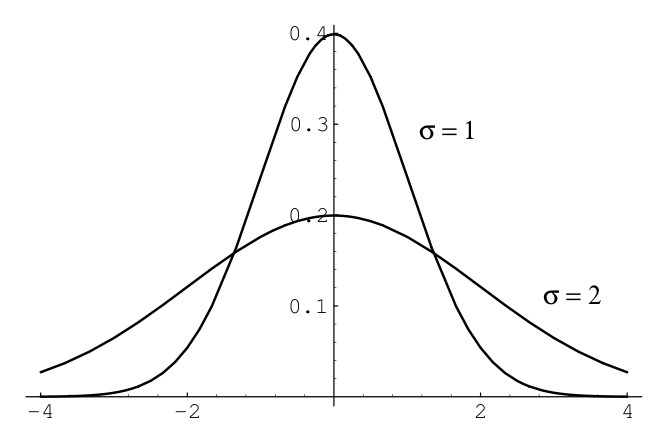
\includegraphics[width=0.6\columnwidth]{figs/intro/normal.png}
  \caption{\label{fig:normaldist} Normal density for two sets of parameter values.}
\end{center}
\end{figure}

Figure \ref{fig:normaldist} compares a plot of normal density for the cases $\mu=0$ and $\sigma=1$, and 
$\mu=0$ and  $\sigma=2$.


\subsection{Maximum Likelihood Estimation}
Until now we assumed that, for every distribution, the parameters $\theta$ are known and are used when we calculate $p(x|\theta)$. There are some cases where the values of the parameters are easy to infer, such as the probability $p$ of getting a head using a fair coin, used on a Bernoulli or Binomial distribution. However, in many problems, these values are complex to define and it is more viable to estimate the parameters using the data $x$. For instance, in the example above with the coin toss, if the coin is somehow tampered to have a biased behavior, rather than examining the dynamics or the structure of the coin to infer a parameter for $p$, a person could simply throw the coin $n$ times, count the number of heads $h$ and set $p=\frac{h}{n}$. By doing so, the person is using the data $x$ to estimate $\theta$.

With this in mind, we will now generalize this process by defining the probability $p(\theta|x)$ as the probability of the parameter $\theta$, given the data $x$. This probability is called {\bf likelihood} $\likelihood(\theta|x)$ and measures how well the parameter $\theta$ models the data $x$. The likelihood can be defined in terms of the distribution $f$ as
\begin{equation*}
\likelihood(\theta|x_1,...,x_n)=\prod_{i=1}^n f(x_i|\theta)
\end{equation*}
where $x_1,...,x_n$ are independently and identically distributed (i.i.d.) samples.

To understand this concept better, we go back to the tampered coin example again. Suppose that we throw the coin 5 times and get the sequence [1,1,1,1,1] (1=head, 0=tail). Using the Bernoulli distribution (see Section~\ref{bernoulli-eq}) $f$ to model this problem, we get the following likelihood values:
\begin{itemize}
\item $\likelihood(0,x) = f(1,0)^5 = 0^5 = 0$
\item $\likelihood(0.2,x) = f(1,0.2)^5 = 0.2^5 = 0.00032$
\item $\likelihood(0.4,x) = f(1,0.4)^5 = 0.4^5 = 0.01024$
\item $\likelihood(0.6,x) = f(1,0.6)^5 = 0.6^5 = 0.07776$
\item $\likelihood(0.8,x) = f(1,0.8)^5 = 0.8^5 = 0.32768$
\item $\likelihood(1,x) = f(1,1)^5 = 1^5 = 1$
\end{itemize}

If we get the sequence [1,0,1,1,0] instead, the likelihood values would be:
\begin{itemize}
\item $\likelihood(0,x) = f(1,0)^3f(0,0)^2 = 0^3\times 1^2 = 0$
\item $\likelihood(0.2,x) = f(1,0.2)^3f(0,0.2)^2 = 0.2^3\times 0.8^2 = 0.00512$
\item $\likelihood(0.4,x) = f(1,0.4)^3f(0,0.4)^2 = 0.4^3\times 0.6^2 = 0.02304$
\item $\likelihood(0.6,x) = f(1,0.6)^3f(0,0.6)^2 = 0.6^3\times 0.4^2 = 0.03456$
\item $\likelihood(0.8,x) = f(1,0.8)^3f(0,0.8)^2 = 0.8^3\times 0.2^2 = 0.02048$
\item $\likelihood(1,x) = f(1,1)^5 = 1^3\times 0^2 = 0$
\end{itemize}

We can see that the likelihood is the highest when the distribution $f$ with parameter $p$ is the best fit for the observed samples. Thus, the best estimate for $p$ according to $x$ would be the value for which $\likelihood(p,x)$ is the highest. 

The value of the parameter $\theta$ with the highest likelihood is called {\bf maximum likelihood estimate (MLE)} and is defined as
\begin{equation*}
\hat{\theta}_{mle}=argmax_{\theta}\likelihood(\theta|x)
\end{equation*}

Finding this for our example is relatively easy, since we can simply derivate the likelihood function to find the absolute maximum. For the sequence [1,0,1,1,0], the likelihood would be given as
\begin{equation*}
\likelihood(p,x) = f(1,p)^3f(0,p)^2 = p^3(1-p)^2
\end{equation*}

And the MLE estimate would be given by:
\begin{equation*}
\frac{\delta \likelihood(p,x)}{\delta p}=0
\end{equation*}
which resolves to
\begin{equation*}
p_{mle}=0.6
\end{equation*}

\begin{exercise}
Over the next couple of exercises we will make use of the Galton dataset, a dataset of heights of fathers and sons from the 1877 paper that first discussed the ``regression to the mean'' phenomenon. This dataset has 928 pairs of numbers.
\begin{itemize}
\item Use the \texttt{load()} function in the \texttt{galton.py} file to load the dataset. The file is located under the \texttt{lxmls/readers} folder. Type the following in your Python interpreter:
\begin{verbatim}
import galton as galton
GaltonData = galton.load()
\end{verbatim}
\item What are the mean height and standard deviation of all the people in the sample? What is the mean height of the fathers and of the sons?
\item Plot a histogram of all the heights (you might want to use the \texttt{plt.hist} function and the \texttt{ravel} method on arrays).
\item Plot the height of the father versus the height of the son.
\item You should notice that there are several points that are exactly the same (e.g., there are 21 pairs with the values 68.5 and 70.2). Use the \texttt{?} command in ipython to read the documentation for the \texttt{numpy.random.randn} function and add random jitter (i.e., move the point a little bit) to the points before displaying them. Does your impression of the data change?
\end{itemize}
\end{exercise}

\subsection{Conjugate Priors}
%\fbox
%{\begin{minipage}[h]{0.9\linewidth} 
\begin{definition}
let $\mathcal{F}= \{f_{X}(x|s), s \in \mathcal{X}\}$ be a class of likelihood functions; let $\mathcal{P}$ be a class of probability (density or mass) functions; if, for any $x$, any $p_{S}(s) \in \mathcal{P}$, and any $f_{X}(x|s) \in \mathcal{F}$, the resulting a posteriori probability function $p_{S}(s|x) = f_{X}(x|s)p_{S}(s)$ is still in $\mathcal{P}$, then $\mathcal{P}$ is called a conjugate family, or a family of {\bf conjugate priors}, for $\mathcal{F}$.
\end{definition}
%\end{minipage}}
%\gka{An example here for conjugate families}


\section{Numerical optimization\label{numerical_optimization}}
Most problems in machine learning require minimization/maximization of functions (likelihoods, risk, energy, entropy, etc.,). Let $x^*$ be the value of $x$ which minimizes the value of some function $f(x)$. Mathematically, this is written as

\begin{equation*}
x^* = \argmin_x f(x)
\end{equation*}

In a few special cases, we can solve this minimization problem analytically in closed form (solving for optimal $x^{*}$ in  $\nabla_{x}f(x^{*})=0$), but in most cases it is too cumbersome (or impossible) to solve these equations analytically, and they must be tackled numerically. In this section we will cover some basic notions of numerical optimization. The goal is to provide the intuitions behind the methods that will be used in the rest of the school. There are plenty of good textbooks in the subject that you can consult for more information \citep{Nocedal1999,bertsekas1995np,boyd2004convex}.

The most common way to solve the problems when no closed form solution is available is to resort to an iterative algorithm. In this Section, we will see some of these iterative optimization techniques. These iterative algorithms construct a sequence of points $x^{(0)},x^{(1)},\ldots \in \text{domain}(f)$ such that hopefully $x^t = x^*$ after a number of iterations.
Such a sequence is called the {\bf minimizing sequence} for the problem.

\subsection{Convex Functions}

One important property of a function $f(x)$ is whether it is a \textbf{convex function} (in the shape of a bowl) or a \textbf{non-convex function}. Figures \ref{fig:convexfn} and \ref{fig:nonconvexfn} show an example of a convex and a non-convex function. Convex functions are particularly useful since you can guarantee that the minimizing sequence converges to the true global minimum of the function, while in non-convex functions you can only guarantee that it will reach a local minimum. 


 \begin{figure}[h]
 \begin{center}
     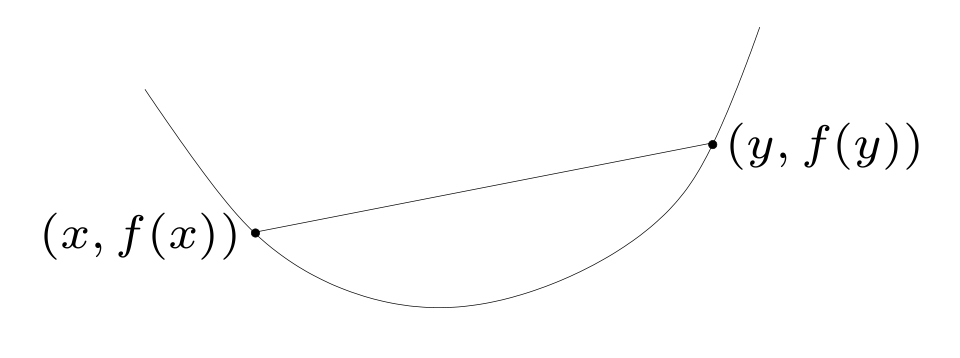
\includegraphics[width=0.6\columnwidth]{figs/intro/convexfn.png}
   \caption{\label{fig:convexfn} Illustration of a convex function. The line segment between any two points on the graph lies entirely above the curve.} 
     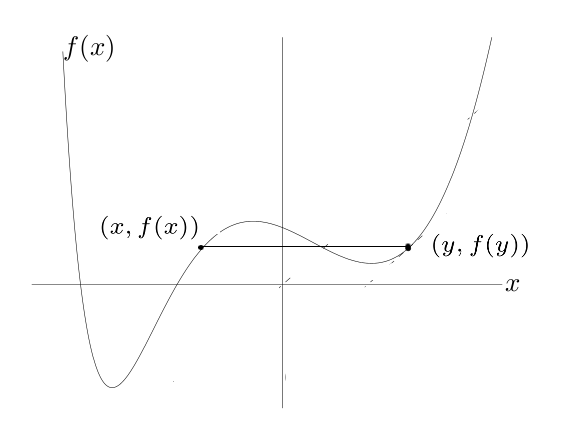
\includegraphics[width=0.5\columnwidth]{figs/intro/nonconvexfn.png}
   \caption{\label{fig:nonconvexfn} Illustration of a non-convex function. Note the line segment intersecting the curve. } 
 \end{center}
 \end{figure}


Intuitively, imagine dropping a ball on either side of Figure \ref{fig:convexfn}, the ball will roll to the bottom of the bowl independently from where it is dropped. This is the main benefit of a convex function. On the other hand, if you drop a ball from the left side of Figure \ref{fig:nonconvexfn} it will reach a different position than if you drop a ball from its right side. Moreover, dropping it from the left side will lead you to a much better (\emph{i.e.}, lower) place than if you drop the ball from the right side. This is the main problem with non-convex functions: there are no guarantees about the quality of the local minimum you find.

More formally, some concepts to understand about convex functions are:

\noindent A {\bf line segment} between points $x_{1}$ and $x_{2}$: contains all points such that 
\begin{equation*}
x=\theta x_{1} + (1-\theta)x_{2}
\end{equation*}
where $0\leq \theta \leq 1$.

\vspace{0.1in}
\noindent A {\bf convex set} contains the line segment between any two points in the set 
\begin{equation*}
x_{1}, x_{2} \in C,\hspace{0.12in} 0 \leq \theta \leq 1 \hspace{0.12in} \Rightarrow \hspace{0.12in} \theta x_{1} + (1-\theta)x_{2} \in C.
\end{equation*}

\vspace{0.1in}
\noindent A function $f: \mathbb{R}^{n}\rightarrow R$ is a {\bf convex function} if the domain of $f$ is a convex set and 
\begin{equation*}
f(\theta x + (1-\theta) y) \leq \theta f(x) + (1-\theta) f(y)
\end{equation*}

\noindent for all $x,y \in \text{domain of } f$, $0 \leq \theta \leq 1$

\subsection{Derivative and Gradient}

The \textbf{derivative} of a function is a measure of how the function varies with its input variables. Given an interval $[a,b]$ one can compute how the function varies within that interval by calculating the average slope of the function in that interval: 
\begin{equation}
\frac{f(b) - f(a)}{b-a}.
\end{equation}
The derivative can be seen as the limit as the interval goes to zero, and it gives us the slope of the function at that point.
\begin{equation}
\frac {\partial f}{\partial x} = \lim_{h = 0} \frac{f(x+h) - f(x)}{h} 
\end{equation}

\noindent Table \ref{tb::derivatives} shows derivatives of some functions that we will be using during the school.

\begin{table}[!h]
\begin{center}
\begin{tabular}{|l|l|}
\hline
Function $f(x)$& Derivative $\frac{\partial f}{\partial x}$\\
\hline
$x^2$ & $2x$\\
\hline
$x^n$ & $nx^{n-1}$\\
\hline
$\log(x)$ & $\frac{1}{x}$\\
\hline
$\exp(x)$ & $\exp(x)$\\
\hline
$\frac{1}{x}$ & $-\frac{1}{x^{2}}$\\
\hline
\end{tabular}
\end{center}
\caption{\label{tb::derivatives}Some derivative examples}
\end{table}

An important rule of derivation is the chain rule. Consider $h=f\circ g$, and $u=g(x)$, then:

\begin{equation}
\frac{\partial h}{\partial x}=\frac{\partial f}{\partial u}\cdot\frac{\partial g}{\partial x}
\end{equation}

\begin{example}

Consider the function $h(x)=\exp(x^{2})$, this can be decomposed as $h(x)=f(g(x))=f(u)=\exp(u)$, where $u=g(x)=x^{2}$ and has derivative $\frac{\partial h}{\partial x}=\frac{\partial f}{\partial u}\cdot \frac{\partial u}{\partial x}=\exp(u) \cdot 2x=\exp(x^{2}) \cdot 2x$

\end{example}

\begin{exercise}
Consider the function $f(x) = x^2$ and its derivative $\frac{\partial f} {\partial x}$. Look at the derivative of that function at points [-2,0,2], draw the tangent to the graph in that point $\frac{\partial f}{\partial x}\left(-2\right)=-4$, $\frac{\partial f}{\partial x}\left(0\right)=0$, and $\frac{\partial f}{\partial x}\left(2\right)=4$. For example, the tangent equation for $x=-2$ is $y=-4x - b$, where $b=f(-2)$. The following code plots the function and the derivatives on those points using matplotlib (See Figure \ref{fig:tangents}).

\begin{python}
a = np.arange(-5,5,0.01)
f_x = np.power(a,2)
plt.plot(a,f_x)

plt.xlim(-5,5)
plt.ylim(-5,15)

k= np.array([-2,0,2])
plt.plot(k,k**2,"bo")
for i in k:
    plt.plot(a, (2*i)*a - (i**2))

\end{python}

\begin{figure}[h]
\begin{center}
   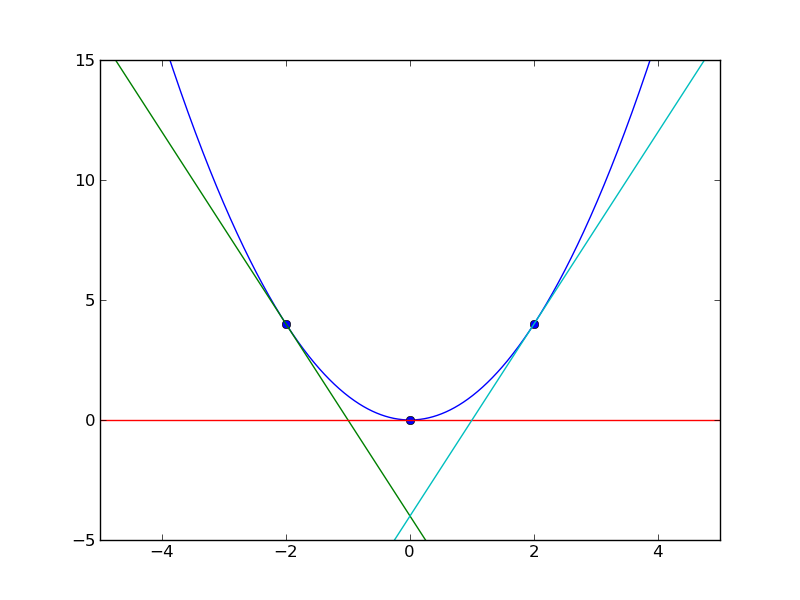
\includegraphics[width=0.6\columnwidth]{figs/intro/tangents.png}
 \caption{\label{fig:tangents} Illustration of the gradient of the
   function $f(x^2)$ at three different points $x = [-2,0.2]$. Note
   that at point $x = 0$ the gradient is zero which corresponds to the
 minimum of the function.}
\end{center}
\end{figure}

\end{exercise}

The \textbf{gradient} of a function is a generalization of the derivative concept we just saw before for several dimensions. Lets assume we have a function  $f(x)$ where $x \in \mathbb{R}^2$, so $x$ can be seen as a pair $x = [{x_1,x_2}]$. Then, the gradient measures the slope of the function in both directions: $\nabla_{x} f(x) = [\frac {\partial f}{\partial x_1},\frac {\partial f}{\partial x_2}]$.

\subsection{\label{gradient_methods} Gradient Based Methods}

Gradient based methods are probably the most common methods used for finding the minimizing sequence for a given function. The methods used in this class will make use of the function value $f(x)$ as well as the gradient of the function $\nabla_{x} f(x)$. The simplest method is the {\bf Gradient descent} method, an unconstrained first-order optimization algorithm.

The intuition of this method is as follows: You start at a given point $x_0$ and compute the gradient at that point $\nabla_{x_0} f(x)$. You then take a step of length $\eta$ on the direction of the negative gradient to find a new point: $x_1$ = $x_0 - \eta \nabla_{x_{0}}
f(x)$. Then, you compute the gradient at this new point, $\nabla_{x_1} f(x)$, and take a step of length $\eta$ on the direction of the negative gradient to find a new point: $x_2$ = $x_1 - \eta \nabla_{x_{1}} f(x)$. You proceed until you have reached a minimum (local or global). Recall from the previous subsection that you can identify the minimum by testing if the norm of the gradient is zero: $||\nabla f(x)|| = 0$.

There are several practical concerns even with this basic algorithm to ensure both that the algorithm converges (reaches the minimum) and that it does so in a fast way (by fast we mean the number of function and gradient evaluations).

\begin{itemize}
\item \textbf{Step Size $\eta$} A first question is how to find the step length $\eta$. One condition is that $eta$ should guarantee sufficient decrease in the function value. We will not cover these methods here but the most common ones are \textbf{Backtracking line search} or the \textbf{Wolf Line Search} \citep{Nocedal1999}.
\item \textbf{Descent Direction}  A second problem is that using the negative gradient as direction can lead to a very slow convergence. Different methods that change the descent direction by multiplying the gradient by a matrix $\beta$ have been proposed that guarantee a faster convergence. Two notable methods are the Conjugate Gradient (CG) and the Limited Memory Quasi Newton methods (LBFGS) \citep{Nocedal1999}.
\item \textbf{Stopping Criteria} Finally, it will normally not be possible to reach full convergence either because it will be too slow, or because of numerical issues (computers cannot perform exact arithmetic). So normally we need to define a stopping criteria for the algorithm. Three common criteria (that are normally used together) are: a maximum number of iterations; the gradient norm be smaller than a given threshold   $||\nabla f(x)|| \leq \eta_1$, or the normalized difference in the function value be smaller than a given threshold $\frac{|f(x_t) - f(x_{t-1})|}{\max(|f(x_t)|,|f(x_{t-1})|)} \leq \eta_2$
\end{itemize}

Algorithm \ref{alg:graddescent} shows the general gradient based algorithm. Note that for the simple gradient descent algorithm $\beta$ is the identity matrix and the descent direction is just the negative gradient of the function, $\beta = -\nabla f(x)$. Figure \ref{fig:graddescent} shows an illustration of the gradient descent algorithm.

\begin{algorithm}[h]
\caption{Gradient Descent\label{alg:graddescent}}
\begin{algorithmic}[1]
\STATE {\bf given} a starting point $x_{0}, i=0$
\STATE {\bf repeat}
\STATE \quad Compute step size $\eta$
\STATE \quad Compute descent direction $- \beta\nabla f(x_{i})$.
\STATE \quad $x_{i+1} \leftarrow x_{i} - \eta\beta\nabla f(x_{i})$
\STATE \quad $i \leftarrow i + 1$
\STATE {\bf until} stopping criterion is satisfied.
\end{algorithmic}
\end{algorithm}

\begin{figure}[h]
\begin{center}
   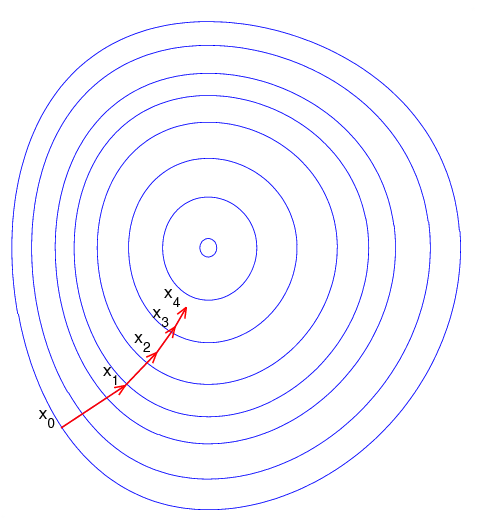
\includegraphics[width=0.6\columnwidth]{figs/intro/graddescent.png}
 \caption{\label{fig:graddescent} Illustration of gradient descent. The blue circles correspond to contours of the function (each blue circle is a set of points which have the same function value), while the red lines correspond to steps taken in the negative gradient direction.}
\end{center}
\end{figure}

% Gradient descent can work in any number of dimensions.  The process can also include {\bf line search} 
% to determine the locally optimal $\eta$ in each iteration. For non-differentiable functions, gradient 
% methods are ill-defined. Also, the procedure can take many iterations to converge to a local minimum 
% and methods based on Newton's method can be better alternatives. The main idea behind
% the iterative minimization techniques is find the locally best direction to move towards the (unknown) minimum. 
% While gradient descent moves in the direction of the negative gradient, other techniques like steepest 
% descent, conjugate descent, (L-)BGFS etc use other directions for update.

\begin{exercise}
Consider the function $f(x) = (x+2)^2 - 16 \exp\left( -(x-2)^2 \right)$.
Make a function that computes the function value given $x$.

\begin{python}
def get_y(x):
    return (x+2)**2 - 16*np.exp(-((x-2)**2))
\end{python}

Draw a plot around $x \in [-8,8]$.

\begin{python}
x = np.arange(-8,8,0.001)
y = map(lambda u: get_y(u),x)
plt.plot(x,y)
plt.show()
\end{python}

Calculate the derivative of the function $f(x)$, implement the function \emph{get\_grad(x)}.

\begin{python}
def get_grad(x):
    return (2*x+4)-16*(-2*x + 4)*np.exp(-((x-2)**2))
\end{python}

Use the method \emph{gradient\_descent} to find the minimum of this function. Convince yourself that the code is doing the proper thing. Look at the constants we defined. Note, that we are using a simple approach to pick the step size (always have the value step\_size) which is not necessarily correct.

\begin{python}
def gradient_descent(start_x,func,grad):
    # Precision of the solution
    prec = 0.0001
    #Use a fixed small step size
    step_size = 0.1
    #max iterations
    max_iter = 100
    x_new = start_x
    res = []
    for i in xrange(max_iter):
        x_old = x_new
        #Use beta egual to -1 for gradient descent 
        x_new = x_old - step_size * grad(x_new)
        f_x_new = func(x_new)
        f_x_old = func(x_old)
        res.append([x_new,f_x_new])
        if(abs(f_x_new - f_x_old) < prec):
            print "change in function values too small, leaving"
            return np.array(res)
    print "exceeded maximum number of iterations, leaving"
    return np.array(res)
\end{python}

Run the gradient descent algorithm starting from $x_0 = -8$ and plot the minimizing sequence.

\begin{python}
x_0 = -8
res = gradient_descent(x_0,get_y,get_grad)
plt.plot(res[:,0],res[:,1],'+')
plt.show()
\end{python}


\begin{figure}[h]
\begin{center}
   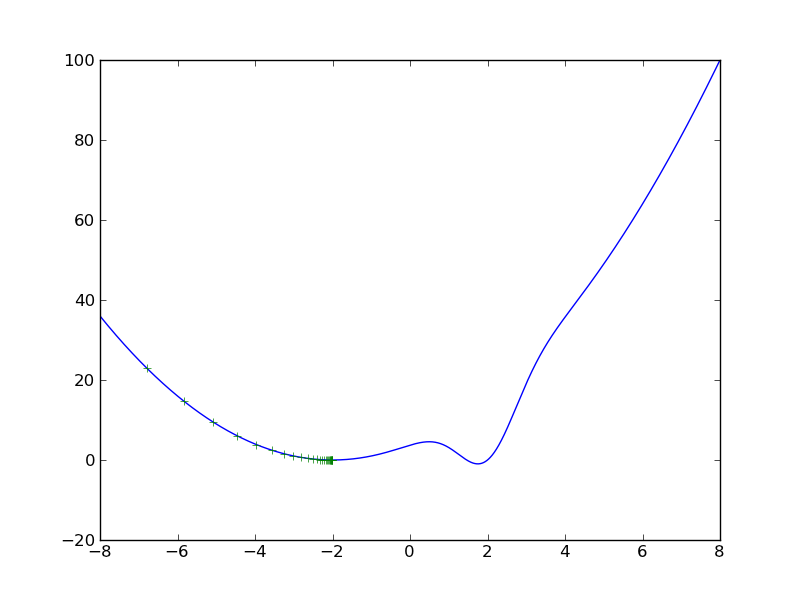
\includegraphics[width=1\columnwidth]{figs/intro/gradex1.png}
 \caption{\label{fig:gradex1} Example of running gradient descent
   starting on point $x_0 = -8$ for function $f(x) = (x+2)^2 - 16
   \exp\left( -(x-2)^2 \right)$. The function is represented in blue,
   while the points of the minimizing sequence are displayed as green
   plus signs.}
\end{center}
\end{figure}


Figure \ref{fig:gradex1} shows the resulting minimizing sequence. Note that the algorithm converged to a minimum, but since the function is not convex it converged only to a local minimum.

Now try the same exercise starting from the initial point $x_0 = 8$.

\begin{python}
x_0 = 8
res = gradient_descent(x_0,get_y,get_grad)
plot(res[:,0],res[:,1],'+')
\end{python}


\begin{figure}[h]
\begin{center}
   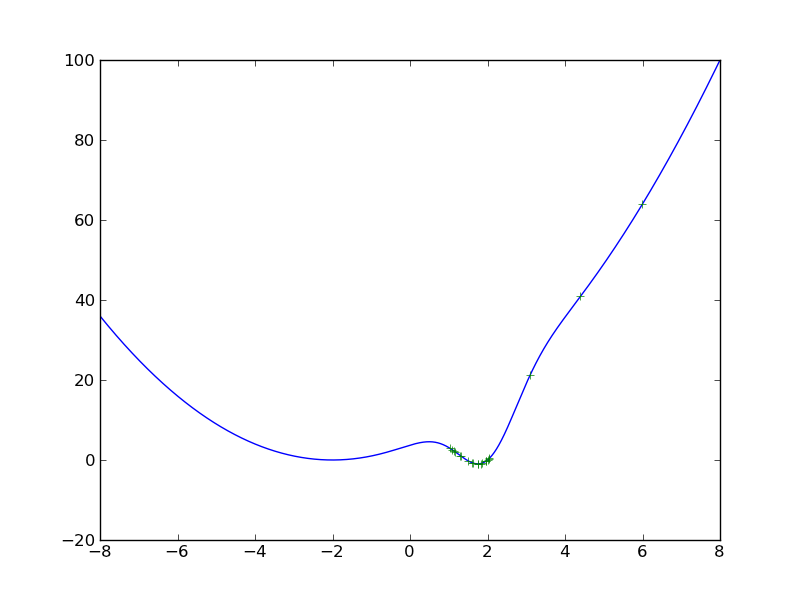
\includegraphics[width=1\columnwidth]{figs/intro/gradex2.png}
 \caption{\label{fig:gradex2} Example of running gradient descent
   starting on point $x_0 = 8$ for function $f(x) = (x+2)^2 - 16
   \exp\left( -(x-2)^2 \right)$. The function is represented in blue,
   while the points of the minimizing sequence are displayed as green
   plus signs.}
\end{center}
\end{figure}


Figure \ref{fig:gradex2} shows the resulting minimizing sequence. Note that now the algorithm converged to the global minimum. However, note that to get to the global minimum the sequence of points jumped from one side of the minimum to the other. This is a consequence of using a wrong step size (in this case too large). Repeat the previous exercise changing both the values of the step-size and the precision. What do you observe?
\end{exercise}

During this school we will rely on the numerical optimization methods provided by Scipy (scientific computing library in python), which are very efficient implementations.


% \begin{exercise}
% Consider the linear regression problem (ordinary least squares), with a
% single response variable

% \[
% y = x^T w + \varepsilon
% \]

% The \emph{linear regression problem} is, given a set $\{ y^{(i)} \}_i$ of
% samples of $y$ and the corresponding $\vect{x}^{(i)}$ vectors, estimate
% $\vect{w}$ to minimise the sum of the $\varepsilon$ variables. Traditionally
% this is solved analytically to obtain a closed form solution (although this is
% \textbf{not the way in which it should be computed}, linear algebra packages
% have an optimised solver, with numpy, use \code{numpy.linalg.lstsq}).

% Alternatively, we can define the error function for each possible $\vect{w}$:

% \[
% e(\vect{w}) = \sum_i \left( {\vect{x}^{(i)}}^T \vect{w} - y^{(i)} \right)^2.
% \]

% \begin{enumerate}
% \item Derive the gradient of the error $\pd{e}{w_j}$.
% \item Implement a solver based on this for two dimensional problems (i.e.,
% $\vect{w} \in R^2$).
% \item Use this method on the Galton dataset from the previous exercise to
% estimate the relationship between father and son's height. Try two formulas
% \begin{equation}
% s = f w_1 + \varepsilon,
% \label{}
% \end{equation}
% where $s$ is the son's height, and $f$ is the father heights; and
% \begin{equation}
% s = f w_1 + 1w_0 + \varepsilon
% \label{}
% \end{equation}
% where the input variable is now two dimensional: $(f,1)$. This allows the
% intercept to be non-zero.
% \item Plot the regression line you obtain with the points from the previous
% exercise.
% \item Use the \texttt{np.linalg.lstsq} function and compare to your solution.
% \end{enumerate}
% \end{exercise}



%Basic concepts of numerical optimization.

%\begin{itemize}
%\item - Gradient base methods, gradient descent, its problems,
%  conjugate and lbfgs. Can use routines from python, make example with
%  Gaussian with different variates and show the behavior.
%\item convex functions vs non convex functions, very brief, convex
%  function is like a bowl, if you drop a ball from the top it will
%  reach the bottom, Non-convex several bottom, will reach one of them.
%\item Gradient, sub-gradient generalization
%\end{itemize}


% \subsection{Matrix Derivatives}

% In subsection we finalize by showing some basic formulas for the
% gradient of matrix:

% \begin{itemize}
% \item For vectors $a$ and $x$, $\frac{\partial a^{T} x}{\partial x}= a$
% \item For vectors $a$ and $x$ and matrix $A$, $\frac{\partial a^{T}Ab}{\partial A} = ab^{T}$
% \item For vectors $a$ and $x$ and matrix $A$, $\frac{\partial a^{T}A^{T}b}{\partial A} =  ba^{T}$
% \end{itemize}

% {\bf The Gradient: }Suppose that $f:\mathbb{R}^{m\times n} \rightarrow\mathbb{R}$ is a function that takes as input, a matrix $A$
% of size $m\times n$ and returns a real value. Then the {\bf gradient} of $f$ (with respect to $A\in \mathbb{R}^{m\times n}$)
% is the matrix of partial derivatives, defined as:
% \begin{equation*}
% \nabla_{A}f(A)\in \mathbb{R}^{m\times n} = \left[\begin{array}{cccc}
% \frac{\partial f(A)}{\partial A_{11}} & \frac{\partial f(A)}{\partial A_{12}} & \ldots & \frac{\partial f(A)}{\partial A_{1n}} \\
% \frac{\partial f(A)}{\partial A_{21}} & \frac{\partial f(A)}{\partial A_{22}} & \ldots & \frac{\partial f(A)}{\partial A_{2n}} \\
% \vdots & \vdots &\ddots & \vdots \\
% \frac{\partial f(A)}{\partial A_{m1}} & \frac{\partial f(A)}{\partial A_{m2}} & \ldots & \frac{\partial f(A)}{\partial A_{mn}} \\
% \end{array}\right].
% \end{equation*}

% The gradient is defined {\em only} if the function is real-valued, that is, if it returns a scalar value. Some 
% important properties:

% \begin{itemize}
% \item $\nabla_{x}(f(x) + g(x)) = \nabla_{x}f(x) + \nabla_{x}g(x)$.
% \item For $t \in \mathbb{R}$, $\nabla_{x}(tf(x))= t\nabla_{x}f(x)$.
% \item Let $f:\mathbb{R}^{m} \rightarrow \mathbb{R}$ be the function defined by $f(z)=z^{T}z$, $\nabla_{z}f(z)=2z$.
% \end{itemize}
% {\bf The Hessian:} Suppose that $f:\mathbb{R}^{n}\rightarrow\mathbb{R}$ is a function that takes a vector in $\mathbb{R}^{n}$ and
% returns a real number, then the {\em Hessian} matrix with respect to $x$, written $\nabla_{x}^{2}f(x)$ (or $H$) is the $n\times n$
% matrix of partial derivatives,

% \begin{equation*}
% \nabla_{x}^{2}f(x) \in \mathbb{R}^{n\times n}= \left[\begin{array}{cccc}
% \frac{\partial^{2}f(x)}{\partial x_{1}^{2}} & \frac{\partial^{2}f(x)}{\partial x_{1} \partial x_{2}} & \ldots &  \frac{\partial^{2}f(x)}{\partial x_{1} \partial x_{n}} \\
% \frac{\partial^{2}f(x)}{\partial x_{2} \partial x_{1}} & \frac{\partial^{2}f(x)}{\partial x_{2}^{2}} & \ldots &  \frac{\partial^{2}f(x)}{\partial x_{2} \partial x_{n}} \\
% \vdots & \vdots & \ddots & \vdots \\
% \frac{\partial^{2}f(x)}{\partial x_{n} \partial x_{1}} & \frac{\partial^{2}f(x)}{\partial x_{n}\partial x_{2}} & \ldots &  \frac{\partial^{2}f(x)}{\partial x_{n}^{2}} 

% \end{array}\right].
% \end{equation*}

% Note that the Hessian is always symmetric, since
% \begin{equation*}
% \frac{\partial^{2}f(x)}{\partial x_{i}\partial x_{j}} =\frac{\partial^{2}f(x)}{\partial x_{j}\partial x_{i}}.
% \end{equation*}



%%% Local Variables: 
%%% mode: latex
%%% TeX-master: "../../guide"
%%% End: 


\section{Python Exercises}




\subsection{Numpy and Matplotlib}

%As discussed in the lecture, there are many helpful functions in numpy. For basic mathematical operations, we have \code{np.log}, \code{np.exp}, \code{np.cos},\ldots with the expected meaning. These operate both on single arguments and on arrays (where they will behave element wise).

%\begin{python}
%import matplotlib.pyplot as plt
%import numpy as np
%X = np.linspace(0, 4 * np.pi, 1000)
%C = np.cos(X)
%S = np.sin(X)

%plt.plot(X, C)
%plt.plot(X, S)
%\end{python}

%Other functions take a whole array and compute a single value from it. For
%example, \code{np.sum}, \code{np.mean},\ldots These are available as both free
%functions and as methods on arrays.

%\begin{python}
%import numpy as np
%A = np.arange(100)
%print np.mean(A)
%print A.mean()

%C = np.cos(A)
%print C.ptp()
%\end{python}

%\begin{exercise}
%Run the above example and lookup the \code{ptp} function/method.
%\end{exercise}

%\begin{exercise}
%Consider the following approximation to compute an integral

%\[
%\int_0^{1} f(x)dx \approx \sum_{i = 0}^{999} \frac{f(i/1000)}{1000}.
%\]

%Use numpy to implement this for $f(x) = x^2$. You should not need to use any
%loops.
%\end{exercise}

%\begin{exercise}
%\begin{enumerate}
%\item Consider the function $f(x) = (x+2)^2 - 16 \exp\left( -(x-2)^2 \right)$.
%Draw a plot around the $x \in [-8,8]$ region.
%\item What is $\pd{f}{x}$?
%\item Use gradient descent to find a local minimum starting from $x_0 = -4$ and
%$x_0 = +4$, with $\eta = .01$. Plot all of the intermediate estimates that you
%obtain in the same plot.
%\end{enumerate}
%\begin{python}
%import numpy as np
%import matplotlib.pyplot as plt
%X = np.linspace(-8, 8, 1000)
%Y = (X+2)**2 - 16*np.exp(-((X-2)**2))
%
%# derivative of the function f
%def get_Y_dev(x):
%    return (2*x+4)-16*(-2*x + 4)*np.exp(-((x-2)**2))
%
%def grad_desc(start_x, eps, prec):
%    '''
%    runs the gradient descent algorithm and returns the list of estimates
%
%    example of use grad_desc(start_x=3.9, eps=0.01, prec=0.00001)
%    '''
%    x_new = start_x
%    x_old = start_x + prec * 2
%    res = [x_new]
%    while abs(x_old-x_new) > prec:
%        x_old = x_new
%        x_new = x_old - eps * get_Y_dev(x_new)
%        res.append(x_new)
%    return np.array(res)
%\end{python}
%\end{exercise}

%Over the next couple of exercises we will make use of the Galton dataset, a
%dataset of heights of fathers and sons from the 1877 paper that first discussed
%the ``regression to the mean'' phenomenon.
%
%\begin{exercise}
%\begin{itemize}
%\item Use the \texttt{load()} function in the \texttt{galton.py} file to load
%the dataset.
%\item What are the mean height and standard deviation of all the people in the
%sample? What is the mean height of the fathers and of the sons?
%\item Plot a histogram of all the heights (you might want to use the
%\texttt{plt.hist} function and the \texttt{ravel} method on arrays).
%\item Plot the height of the father versus the height of the son.
%\item You should notice that there are several points that are exactly the same
%(e.g., there are 21 pairs with the values 68.5 and 70.2). Use the \texttt{?}
%command in ipython to read the documentation for the \texttt{numpy.random.rand}
%function and add random jitter (i.e., move the point a little bit) to the
%points before displaying them. Does your impression of the data change?
%\end{itemize}
%\end{exercise}

\begin{exercise}
Consider the linear regression problem (ordinary least squares) on the Galton
dataset, with a single response variable

\[
y = x^T w + \varepsilon
\].

The \emph{linear regression problem} is, given a set $\{ y^{(i)} \}_i$ of
samples of $y$ and the corresponding $\vect{x}^{(i)}$ vectors, estimate
$\vect{w}$ to minimise the sum of the $\varepsilon$ variables. Traditionally
this is solved analytically to obtain a closed form solution (although this is
\textbf{not the way in which it should be computed} in this exercise, linear algebra packages
have an optimised solver, with numpy, use \code{numpy.linalg.lstsq}).

Alternatively, we can define the error function for each possible $\vect{w}$:

\[
e(\vect{w}) = \sum_i \left( {\vect{x}^{(i)}}^T \vect{w} - y^{(i)} \right)^2.
\]

\begin{enumerate}
\item Derive the gradient of the error $\pd{e}{w_j}$.
\item Implement a solver based on this for two dimensional problems (i.e.,
$\vect{w} \in R^2$).
\item Use this method on the Galton dataset from the previous exercise to
estimate the relationship between father and son's height. Try two formulas
\begin{equation}
s = f w_1 + \varepsilon,
\label{}
\end{equation}
where $s$ is the son's height, and $f$ is the father heights; and
\begin{equation}
s = f w_1 + 1w_0 + \varepsilon
\label{}
\end{equation}
where the input variable is now two dimensional: $(f,1)$. This allows the
intercept to be non-zero.
\item Plot the regression line you obtain with the points from the previous
exercise.
\item Use the \texttt{np.linalg.lstsq} function and compare to your solution.
\end{enumerate}

Please refer to the notebook for solutions.
\end{exercise}

\subsection{Debugging}


\begin{exercise}
Use the debugger to debug the \texttt{buggy.py} script which attempts to
repeatedly perform the following computation:

\begin{enumerate}
\item Start $x_0 = 0$
\item Iterate

\begin{enumerate}
\item $x'_{t+1} = x_t + r$, where $r$ is a random variable.
\item if $x'_{t+1} >= 1.$, then stop.
\item if $x'_{t+1} <= 0.$, then $x_{t+1} = 0$
\item else $x_{t+1} = x'_{t+1}$.
\end{enumerate}
\item Return the number of iterations.
\end{enumerate}

Having repeated this computation a number of times, the programme prints the
average. Unfortunately, the program has a few bugs, which you need to fix.
\end{exercise}




%\section*{Related Exercises in Python}

%\input{pages/day0/ipython}

\section{Python Exercises}





\subsection{Numpy and Matplotlib}

%As discussed in the lecture, there are many helpful functions in numpy. For basic mathematical operations, we have \code{np.log}, \code{np.exp}, \code{np.cos},\ldots with the expected meaning. These operate both on single arguments and on arrays (where they will behave element wise).

%\begin{python}
%import matplotlib.pyplot as plt
%import numpy as np
%X = np.linspace(0, 4 * np.pi, 1000)
%C = np.cos(X)
%S = np.sin(X)

%plt.plot(X, C)
%plt.plot(X, S)
%\end{python}

%Other functions take a whole array and compute a single value from it. For
%example, \code{np.sum}, \code{np.mean},\ldots These are available as both free
%functions and as methods on arrays.

%\begin{python}
%import numpy as np
%A = np.arange(100)
%print np.mean(A)
%print A.mean()

%C = np.cos(A)
%print C.ptp()
%\end{python}

%\begin{exercise}
%Run the above example and lookup the \code{ptp} function/method.
%\end{exercise}

%\begin{exercise}
%Consider the following approximation to compute an integral

%\[
%\int_0^{1} f(x)dx \approx \sum_{i = 0}^{999} \frac{f(i/1000)}{1000}.
%\]

%Use numpy to implement this for $f(x) = x^2$. You should not need to use any
%loops.
%\end{exercise}

\begin{exercise}
\begin{enumerate}
\item Consider the function $f(x) = (x+2)^2 - 16 \exp\left( -(x-2)^2 \right)$.
Draw a plot around the $x \in [-8,8]$ region.
\item What is $\pd{f}{x}$?
\item Use gradient descent to find a local minimum starting from $x_0 = -4$ and
$x_0 = +4$, with $\eta = .01$. Plot all of the intermediate estimates that you
obtain in the same plot.
\end{enumerate}
\begin{python}
import numpy as np
import matplotlib.pyplot as plt
X = np.linspace(-8, 8, 1000)
Y = (X+2)**2 - 16*np.exp(-((X-2)**2))

# derivative of the function f
def get_Y_dev(x):
    return (2*x+4)-16*(-2*x + 4)*np.exp(-((x-2)**2))

def grad_desc(start_x, eps, prec):
    '''
    runs the gradient descent algorithm and returns the list of estimates

    example of use grad_desc(start_x=3.9, eps=0.01, prec=0.00001)
    '''
    x_new = start_x
    x_old = start_x + prec * 2
    res = [x_new]
    while abs(x_old-x_new) > prec:
        x_old = x_new
        x_new = x_old - eps * get_Y_dev(x_new)
        res.append(x_new)
    return np.array(res)
\end{python}
\end{exercise}

%Over the next couple of exercises we will make use of the Galton dataset, a
%dataset of heights of fathers and sons from the 1877 paper that first discussed
%the ``regression to the mean'' phenomenon.
%
%\begin{exercise}
%\begin{itemize}
%\item Use the \texttt{load()} function in the \texttt{galton.py} file to load
%the dataset.
%\item What are the mean height and standard deviation of all the people in the
%sample? What is the mean height of the fathers and of the sons?
%\item Plot a histogram of all the heights (you might want to use the
%\texttt{plt.hist} function and the \texttt{ravel} method on arrays).
%\item Plot the height of the father versus the height of the son.
%\item You should notice that there are several points that are exactly the same
%(e.g., there are 21 pairs with the values 68.5 and 70.2). Use the \texttt{?}
%command in ipython to read the documentation for the \texttt{numpy.random.rand}
%function and add random jitter (i.e., move the point a little bit) to the
%points before displaying them. Does your impression of the data change?
%\end{itemize}
%\end{exercise}

\begin{exercise}
Consider the linear regression problem (ordinary least squares) on the Galton
dataset, with a single response variable

\[
y = x^T w + \varepsilon
\].

The \emph{linear regression problem} is, given a set $\{ y^{(i)} \}_i$ of
samples of $y$ and the corresponding $\vect{x}^{(i)}$ vectors, estimate
$\vect{w}$ to minimise the sum of the $\varepsilon$ variables. Traditionally
this is solved analytically to obtain a closed form solution (although this is
\textbf{not the way in which it should be computed} in this exercise, linear algebra packages
have an optimised solver, with numpy, use \code{numpy.linalg.lstsq}).

Alternatively, we can define the error function for each possible $\vect{w}$:

\[
e(\vect{w}) = \sum_i \left( {\vect{x}^{(i)}}^T \vect{w} - y^{(i)} \right)^2.
\]

\begin{enumerate}
\item Derive the gradient of the error $\pd{e}{w_j}$.
\item Implement a solver based on this for two dimensional problems (i.e.,
$\vect{w} \in R^2$).
\item Use this method on the Galton dataset from the previous exercise to
estimate the relationship between father and son's height. Try two formulas
\begin{equation}
s = f w_1 + \varepsilon,
\label{}
\end{equation}
where $s$ is the son's height, and $f$ is the father heights; and
\begin{equation}
s = f w_1 + 1w_0 + \varepsilon
\label{}
\end{equation}
where the input variable is now two dimensional: $(f,1)$. This allows the
intercept to be non-zero.
\item Plot the regression line you obtain with the points from the previous
exercise.
\item Use the \texttt{np.linalg.lstsq} function and compare to your solution.
\end{enumerate}
\end{exercise}

\subsection{Debugging}


\begin{exercise}
Use the debugger to debug the \texttt{buggy.py} script which attempts to
repeatedly perform the following computation:

\begin{enumerate}
\item Start $x_0 = 0$
\item Iterate

\begin{enumerate}
\item $x'_{t+1} = x_t + r$, where $r$ is a random variable.
\item if $x'_{t+1} >= 1.$, then stop.
\item if $x'_{t+1} <= 0.$, then $x_{t+1} = 0$
\item else $x_{t+1} = x'_{t+1}$.
\end{enumerate}
\item Return the number of iterations.
\end{enumerate}

Having repeated this computation a number of times, the programme prints the
average. Unfortunately, the program has a few bugs, which you need to fix.
\end{exercise}







\chapter{\label{day:classification}Classification}

This day will serve as an introduction to machine learning. We recall some fundamental concepts 
about decision theory and classification. We also present some widely used models and algorithms 
and try to provide the main motivation behind them. 
There are several textbooks that provide a thorough description of some of the concepts introduced here: 
for example, \citet{Mitchell1997},\citet{Duda2001}, \citet{Schoelkopf2002}, \citet{Joachims2002}, \citet{Bishop2006}, \citet{Manning2008}, 
to name just a few.  
The concepts that we introduce in this chapter will be revisited in later chapters, where the same algorithms and models 
will be adapted to structured inputs and outputs. For now, we concern only with multi-class classification 
(with just a few classes). 

\section*{Today's assignment}

The assignment of today's class is to implement a classifier called Naive Bayes, and use it to perform sentiment analysis on a corpus of book reviews from Amazon.

\section{Pre-assignment}

\subsection{Notation}

In what follows, we denote by $\mathcal{X}$ our \emph{input set} (also called \emph{observation set}), and by $\mathcal{Y}$ our \emph{output set}. 
We will make no assumptions about the set $\mathcal{X}$, which can be continuous or discrete. In this lecture, we 
consider \emph{classification} problems, where $\mathcal{Y} = \{c_1,\ldots,c_K\}$ is a finite set, consisting of $K$ \emph{classes} (also called \emph{labels}). 
For example, $\mathcal{X}$ can be a set of documents in natural language, and $\mathcal{Y}$ a set of topics, the goal 
being to assign a topic to each document. 

We use upper-case letters for denoting random variables, and lower-case letters for value assignments to those variables:  
for example, 
\begin{itemize}
\item $X$ is a random variable taking values on $\mathcal{X}$,
\item $Y$ is a random variable taking values on $\mathcal{Y}$,
\item $x \in \mathcal{X}$ and $y \in \mathcal{Y}$ are particular values for $X$ and $Y$. 
\end{itemize}  
We consider \emph{events} such as $X=x$, $Y=y$, etc. 
Throughout, we use modified notation and let $P(y)$ denote the \emph{probability} associated with the event $Y=y$ (instead of writing $P_Y(Y=y)$). 
\emph{Joint} and \emph{conditional} probabilities are 
denoted respectively as $P(x,y) \triangleq P_{X,Y}(X=x \wedge Y=y)$ and $P(x|y) \triangleq P_{X|Y}(X=x \,\,|\,\,Y=y)$. From the laws of probabilities: 
\begin{equation}
P(x,y)=P(y|x) P(x) = P(x|y) P(y), 
\end{equation}
for all $x \in \mathcal{X}$ and $y \in \mathcal{Y}$.

Quantities that are predicted or estimated from the data will be appended a hat-symbol: for example, estimations of the probabilities above are denoted 
as ${\hat P}(y)$, ${\hat P}(x,y)$ and ${\hat P}(y|x)$; and a prediction of an output will be denoted ${\hat y}$. 

We assume that a \emph{training dataset} $\mathcal{D}$ is provided
which consists of $M$ input-output pairs (called \emph{examples} or
\emph{instances}): 
\begin{equation}
\mathcal{D} = \{(x^{1},y^{1}),\ldots,(x^{M},y^{M})\} \subseteq \mathcal{X} \times \mathcal{Y}.  
\end{equation}

The goal of (supervised) machine learning is to use the training dataset $\mathcal{D}$ to learn a function $h$ (called a \emph{classifier}) 
that maps from $\mathcal{X}$ to $\mathcal{Y}$: this way, given a new instance 
$x \in \mathcal{X}$ (test example), the machine makes a prediction ${\hat y}$ by evaluating $h$ on $x$, i.e., ${\hat y} = h(x)$. 

%\out{
\begin{figure}
\begin{center}
    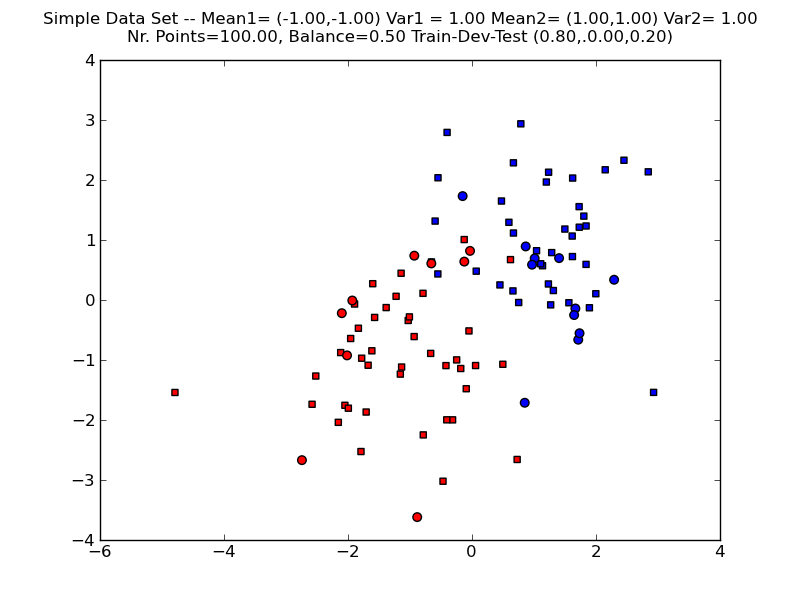
\includegraphics[width=1\columnwidth]{figs/classification/simple_data_set}
  \caption{\label{simpleDataSet} Example of a dataset.
    The input set consists in points in the real plane, $\mathcal{X} =
    \mathbb{R}^2$, and the output set consists of two classes (Red
    and Blue). Training points are represented as squares, while test
    points are represented as circles.}
  \end{center}
\end{figure}
%}

\subsection{\label{s::naiveBayes}Generative Classifiers: Na\"{i}ve Bayes}

If we knew the \emph{true} distribution $P(X,Y)$, the best possible classifier (Bayes optimal) 
would be one which predicts according to

\begin{eqnarray}
{\hat y} &=& \arg\max_{y \in \mathcal{Y}} P(y|x) = \arg\max_{y \in \mathcal{Y}} \frac{P(x,y)}{P(x)} \nonumber\\
&=^{\dagger}& \arg\max_{y \in \mathcal{Y}} P(x,y) \nonumber \\
&=& \arg\max_{y \in \mathcal{Y}} P(y) P(x|y),
\end{eqnarray}
where in ${\dagger}$ we used the fact that $P(x)$ is constant with respect to $y$. Generative classifiers try to estimate the probability distributions $P(Y)$ and $P(X|Y)$ (which are respectively called the \emph{class prior} and the \emph{class conditionals}).
  
Figure \ref{simpleDataSet_bo} shows an example of
the Bayes optimal decision boundary for a toy example with $K=2$ classes, $M=100$ points, class priors $P(y_1) = P(y_2) = 0.5$, and class conditionals $P(x|y_i)$ given by 2-D Gaussian distributions with the same variance but different means.

\begin{figure}[h]
\begin{center}
    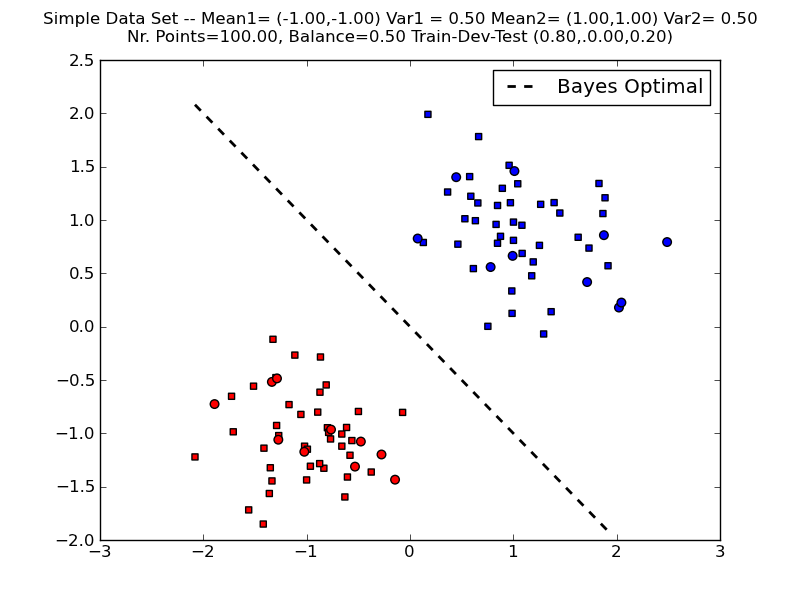
\includegraphics[width=1\columnwidth]{figs/classification/gaussian_separabale_bo.png}
  \caption{\label{simpleDataSet_bo} Example of a dataset together with
    the corresponding Bayes optimal decision boundary.
    The input set consists in points in the real plane, $\mathcal{X} =
    \mathcal{R^2}$, and the output set consists of two classes (Red
    and Blue). Training points are represented as squares, while test
    points are represented as circles.}
  \end{center}
\end{figure}



Generative models assume that the data are generated according to the following generative story (independently for each $m=1,\ldots,M$): 
\begin{enumerate}
\item A class $y_m \sim P(Y)$ is drawn from the class prior distribution;
\item An input $x_m \sim P(X|Y=y_m)$ is drawn from the corresponding class conditional.
\end{enumerate}
Training a generative model 
amounts to \emph{estimating} these probabilities using the dataset $\mathcal{D}$, yielding estimates 
$\hat{P}(y)$ and $\hat{P}(x|y)$. This estimation is usually called \emph{training}, or \emph{learning}.

After we are done training, we are given a new input $x \in \mathcal{X}$, and we want to make a prediction according to  
\begin{eqnarray}
{\hat y} &=& \arg\max_{y \in \mathcal{Y}} \hat{P}(y) \hat{P}(x|y),
\label{eq:argmax}
\end{eqnarray}
using the probabilities estimated in the training stage. This is usually called \emph{inference} or \emph{decoding}.


We are left with two important problems:
\begin{enumerate}
\item How should the distributions ${\hat P}(Y)$ and ${\hat P}(X|Y)$ be ``defined''?
(i.e., what kind of independence assumptions should they state, or how should they factor?)
\item How should parameters be estimated from the training data $\mathcal{D}$?
\end{enumerate}

The first problem strongly depends on the application at hand. Quite often, there is a natural decomposition of the input variable $X$ into $J$ components, 
\begin{equation}
X = (X_1,\ldots,X_J). 
\end{equation}
The na\"{i}ve Bayes method makes the following assumption: \emph{$X_1,\ldots,X_J$ are conditionally independent given the class}. Mathematically, this means that 
\begin{eqnarray}
P(X|Y) &=& \prod_{j=1}^J P(X_j|Y).
\end{eqnarray}
Note that this independence assumption greatly reduces the number of parameters to be estimated (degrees of freedom) 
from $O(\exp(J))$ to $O(J)$, 
hence estimation of ${\hat P}(X|Y)$ becomes much simpler, as we shall see. 
It also makes the overall computation much more efficient for large $J$ and it decreases the risk of overfitting the data. 
On the other hand, if the assumption is over-simplistic it may increase the risk 
of under-fitting. 
%This choice greatly simplifies the problem of parametrizing ${\hat P}(Y)$ and ${\hat P}(X|Y)$. 

For the second problem, one of the simplest ways to solve it is using \emph{maximum likelihood estimation}, which aims to maximize the probability of the training sample, assuming that each point was generated independently. This probability (call it $P(\mathcal{D})$) factorizes as 
\begin{eqnarray}
P(\mathcal{D}) &=& \prod_{m=1}^M P(x^m,y^m) \nonumber\\
&=& \prod_{m=1}^M P(y^m)\prod_{j=1}^J P(x^m_j|y^m). 
\end{eqnarray}



%%\begin{example}[2-D Gaussians] 
%\subsection{Example: 2-D Gaussians}
%
%We first illustrate the na\"ive Bayes assumption with a toy example. 
%Suppose that $\mathcal{X}=\mathbb{R}^2$ and $\mathcal{Y}=\{1,2\}$. 
%Assume that each class-conditional is a two-dimensional Gaussian distribution with fixed covariance, 
%i.e., $P(X_1,X_2|Y=y)=\mathcal{N}(\boldsymbol{\mu}_y, \boldsymbol{\Sigma}_y)$. 
%
%According to the na\"ive Bayes assumption, ${\hat P}(X_1,X_2|Y) = {\hat P}(X_1|Y) {\hat P}(X_2|Y)$ (remark: this 
%is equivalent to assuming that 
%the $\boldsymbol{\Sigma}_y$ are diagonal!). For simplicity, we also assume that the two classes have unit variance. Then, we have 
%${\hat P}(X_1|Y=y) = \mathcal{N}(\mu_{y1}, 1.0)$ 
%and ${\hat P}(X_2|Y=y) = \mathcal{N}(\mu_{y2}, 1.0)$. Figure
%\ref{simpleDataSet} shows an example a dataset of two gaussians with unit
%variance, where $\mu_{y1} = [-1,-1]$ and $\mu_{y1} = [1,1]$. Figure
%\ref{simpleDataSet_bo} shows the same example but where both
%gaussians have $\Sigma = 0.5$, together with the Bayes optimal decision boundary. 
%The parameters that need to be estimated are the class-conditional means $\mu_{11},\mu_{12},\mu_{21},\mu_{22}$ and 
%the class priors ${\hat P}(Y=1)$ and ${\hat P}(Y=2)$. Given a training sample $\mathcal{D} = \{(x^{1},y^{1}),\ldots,(x^{M},y^{M})\}$, 
%denote by $\mathcal{I}_1\subseteq \{1,\ldots,M\}$ the indices of those instances belonging to class $1$, and 
%by $\mathcal{I}_2\subseteq \{1,\ldots,M\}$ the indices of the ones that belong to class $2$. 
%The maximum likelihood estimates of the quantities above are: 
%\begin{eqnarray}
%{\hat P}(Y = 1) = \frac{|\mathcal{I}_1|}{M}, \quad 
%{\hat P}(Y = 2) = \frac{|\mathcal{I}_2|}{M}\nonumber\\
%\mu_{11} = \frac{1}{|\mathcal{I}_1|} \sum_{m \in \mathcal{I}_1} x_1^{m}, \quad
%\mu_{12} = \frac{1}{|\mathcal{I}_1|} \sum_{m \in \mathcal{I}_1} x_2^{m}\nonumber\\
%\mu_{21} = \frac{1}{|\mathcal{I}_2|} \sum_{m \in \mathcal{I}_2} x_1^{m}, \quad
%\mu_{22} = \frac{1}{|\mathcal{I}_2|} \sum_{m \in \mathcal{I}_2} x_2^{m}.
%\end{eqnarray}
%In words: the class priors' estimates are their relative frequencies, and 
%the class-conditional means' estimates are the sample means. 
%%\end{example}
%
%\begin{exercise}\label{exer:simplenb}
%
%\begin{enumerate}
%Start by importing all the libraries necessary for this lab through the following preamble: 
%\begin{python}
%import sys
%import matplotlib.pyplot as plt
%sys.path.append("readers/")
%sys.path.append("classifiers/")
%sys.path.append("distributions/")
%sys.path.append("util/")
%
%import simple_data_set as sds
%import linear_classifier as lcc
%import gaussian_naive_bayes as gnbc
%import naive_bayes as nb
%\end{python}
%
%Now, generate a training and a test dataset like in the previous example, each with $M=100$ points, $50$ of each class. 
%Assume the following class-conditionals: 
%$P(X|Y=1) \sim N((-1,-1), \sigma^2 \boldsymbol{I})$ and $P(X|Y=2) \sim
%N((1,1), \boldsymbol{I})$, for $\sigma = 1.0$. 
%To do this, run the following command from the {\tt code} directory:
%
%\begin{python}
%sd = sds.SimpleDataSet(nr_examples=100, g1 = [[-1,-1],1], g2 = [[1,1],1], balance=0.5, split=[0.5, 0, 0.5])
%\end{python}
%
%You can visualize your data and see the Bayes optimal surface boundary by typing: 
%\begin{python}
%fig,axis = sd.plot_data()
%\end{python}
%
%Note: you might need to type {\tt plt.show()} in order to show the figure.
%
%Now, run na\"ive Bayes on this dataset. To do that, use the class {\tt GaussianNaiveBayes}, 
%which is defined in the file {\tt GaussianNaiveBayes.py} under the
%classification directory. 
%Report your estimates, as well as training set and testing set
%accuracies:
%
%\begin{python}
%gnb = gnbc.GaussianNaiveBayes()
%params_nb_sd = gnb.train(sd.train_X, sd.train_y)
%
%print "Estimated Means"
%print gnb.means
%print "Estimated Priors"
%print gnb.prior
%y_pred_train = gnb.test(sd.train_X,params_nb_sd)
%acc_train = gnb.evaluate(sd.train_y, y_pred_train)
%y_pred_test = gnb.test(sd.test_X,params_nb_sd)
%acc_test = gnb.evaluate(sd.test_y, y_pred_test)
%print "Gaussian Naive Bayes Simple Dataset Accuracy train: %f test: %f"%(acc_train,acc_test)
%\end{python}
%
%To visualize the surface boundary estimated by na\"ive Bayes, type: 
%\begin{python}
%fig,axis = sd.add_line(fig,axis,params_nb_sd,"Naive Bayes","red")
%\end{python}
%Do not worry for now about why the surface boundaries look the way they look. This is going to be the subject of \S\ref{sec:linearclass}. 
%
%
%Repeat the exercise above for different values of $\sigma^2$, different balances, and different sample sizes. What do you observe? 
%
%\end{enumerate}
%\end{exercise}


\subsection{Example: Multinomial Na\"{i}ve Bayes for Document Classification}

We now consider a more realistic scenario where the na\"ive Bayes classifier may be applied. 
Suppose that the task is \emph{document classification}: 
$\mathcal{X}$ is the set of all possible documents, and $\mathcal{Y}=\{y_1,\ldots,y_K\}$ is a set of classes for those documents. 
Let $\mathcal{V} = \{w_1,\ldots,w_J\}$ be the vocabulary, i.e., the set of words that occur in some document. 

A very popular document representation is through a ``bag-of-words'': each document is seen as a collection of words along with 
their frequencies; word ordering is ignored. We are going to see that this is equivalent to a na\"ive Bayes assumption with the \emph{multinomial model}.%
%\footnote{Another popular model for documents is the Bernoulli model, which only looks at the presence/absence of a word in a 
%document, rather than word frequency. See \cite{Manning2008,McCallum1998} for further information.} % 
We associate to each class a multinomial distribution, which ignores word ordering, but takes into consideration the 
frequency with which each word appears in a document. For simplicity, we assume that all documents have the same length $L$.%
\footnote{We can get rid of this assumption by defining a distribution on the document length. Everything stays the same 
if that distribution is uniform up to a maximum document length.} %
Each document $x$ is assumed to have been generated as follows. First, a class $y$ is generated according to $P(y)$. Then, 
$x$ is generated by sequentially picking words from $\mathcal{V}$ with replacement. Each word $w_j$ is picked with probability $P(w_j|y)$. 
For example, the probability of generating a document $x = w_{j_1}\ldots w_{j_L}$ (\emph{i.e.}, a sequence of 
$L$ words $w_{j_1},\ldots,w_{j_L}$) is 
\begin{eqnarray}
P(x|y) = \prod_{l=1}^L P(w_{j_l}|y) = \prod_{j=1}^J P(w_j|y)^{n_j(x)},
\end{eqnarray}
where $n_j(x)$ is the number of occurrences of word $w_j$ in document $x$. 

Hence, the assumption is that word occurrences (\emph{tokens}) are independent given the class. 
The parameters that need to be estimated are ${\hat P}(y_1),\ldots,{\hat P}(y_K)$, and ${\hat P}(w_j|y_k)$ for $j=1,\ldots,J$ and $k=1,\ldots,K$. 
Given a training sample $\mathcal{D} = \{(x^{1},y^{1}),\ldots,(x^{M},y^{M})\}$, 
denote by $\mathcal{I}_k$ the indices of those instances belonging to the $k$th class. 
The maximum likelihood estimates of the quantities above are: 
\begin{eqnarray}\label{eq:mlemultinomial}
{\hat P}(y_k) = \frac{|\mathcal{I}_k|}{M}, \qquad
{\hat P}(w_j|y_k) = \frac{\sum_ {m \in \mathcal{I}_k} n_j(x^m)}{\sum_{i=1}^J \sum_ {m\in \mathcal{I}_k} n_i(x^m)}.
\end{eqnarray}
In words: the class priors' estimates are their relative frequencies (as before), and 
the class-conditional word probabilities are the relative frequencies of those words across documents with that class.


\section{Assignment}

\begin{exercise}
In this exercise we will use the the Amazon sentiment analysis data \citep{blitzer2007biographies}, 
where the goal is to classify text documents as expressing a \emph{positive} or \emph{negative} sentiment 
(i.e., a classification problem with two labels). We are going to focus on book reviews. 
To load the data, type:
\begin{python}
import sentiment_reader as srs
import naive_bayes as nb

scr = srs.SentimentCorpus("books")
\end{python}
This will load the data in a bag-of-words representation where rare words (occurring less than $5$ times in the training data) are removed. 

\begin{enumerate}
\item Open the file {\tt multinomial\_naive\_bayes.py}. Inside the {\tt MultinomialNaiveBayes} class you will find the {\tt train} method. We have already placed some code in that file to help you get started.

\item Run na\"ive Bayes with the multinomial model on the Amazon
  dataset (sentiment classification) and report results both for
  training and testing: 
    
\begin{python}
import multinomial_naive_bayes as mnbb

mnb = mnbb.MultinomialNaiveBayes()
params_nb_sc = mnb.train(scr.train_X,scr.train_y)
y_pred_train = mnb.test(scr.train_X,params_nb_sc)
acc_train = mnb.evaluate(scr.train_y, y_pred_train)
y_pred_test = mnb.test(scr.test_X,params_nb_sc)
acc_test = mnb.evaluate(scr.test_y, y_pred_test)
print "Multinomial Naive Bayes Amazon Sentiment Accuracy train: %f test: %f"%(acc_train,acc_test)  
\end{python}


\item Observe that words that were not observed at training time cause problems at test time. Why? 
To solve this problem, apply a simple \emph{add-one} smoothing technique: replace the expression in Eq.~\ref{eq:mlemultinomial} 
for the estimation of the conditional probabilities 
by
$${\hat P}(w_j|c_k) = \frac{1+\sum_ {m \in \mathcal{I}_k} n_j(x^m)}{J + \sum_{i=1}^J \sum_ {m\in \mathcal{I}_k} n_i(x^m)}.$$
%$${\hat P}(w_j|c_k) = \frac{1+\sum_ {m \in \mathcal{I}_k} n_j(x^m)}{J + |\mathcal{I}_k|}.$$


where $J$ is the number of distinct words. 

This is a widely used smoothing strategy which has a Bayesian interpretation: it corresponds to choosing a uniform prior 
for the word distribution on both classes, and to replace the maximum likelihood criterion by a \emph{maximum a posteriori} approach. 
This is a form of \emph{regularization}, preventing the model from \emph{overfitting} on the training data. 
See \emph{e.g.} \citet{Manning1999,Manning2008} for more information. 
Report the new accuracies. 
\end{enumerate}
\end{exercise}

\section{Post-assignment}

\subsection{Features and Discriminative Classifiers}\label{sec:linearclass}

In the previous sections we discussed generative classifiers. Those classifiers require us to model the class prior and class conditional distributions. Recall, however, that a classifier is \emph{any} function which maps objects $x \in \mathcal{X}$ onto classes $y \in \mathcal{Y}$. While it's often useful to model how the data was generated, it's not required. Classifiers which do not model these distributions are called \emph{discriminative} classifiers. 

For the purpose of understanding discriminative classifiers, it is useful to think about each  $x \in \mathcal{X}$ as an abstract object which is subject to a set of descriptions or measurements, which are called \emph{features}. A feature is simply a real number that describes the value of some property of $x$. For example, in the previous section, the features of a document were the number of times each word $w_j$ appeared in it.

Let $g_1(x),\ldots,g_J(x)$ be $J$ features of $x$. We call the vector
\begin{equation}
\boldsymbol{g}(x) = (g_1(x),\ldots,g_J(x))
\end{equation} 
a \emph{feature vector representation} of $x$. 
The map $\boldsymbol{g}:\mathcal{X}\rightarrow \mathbb{R}^J$ is called a \emph{feature mapping}. 

In NLP applications, features are often binary-valued and result from evaluating propositions such as: 
\begin{eqnarray}
g_1(x) &\triangleq& 
\left\{
\begin{array}{ll}
1, & \text{if sentence $x$ contains the word \emph{Ronaldo}}\\
0, & \text{otherwise.}
\end{array}
\right.\\
g_2(x) &\triangleq& 
\left\{
\begin{array}{ll}
1, & \text{if all words in sentence $x$ are capitalized}\\
0, & \text{otherwise.}
\end{array}
\right.\\
g_3(x) &\triangleq& 
\left\{
\begin{array}{ll}
1, & \text{if $x$ contains any of the words \emph{amazing}, \emph{excellent} or \emph{:-)}}\\
0, & \text{otherwise.}
\end{array}
\right.
\end{eqnarray}  
In this example, the feature vector representation of the sentence "Ronaldo shoots and scores an amazing goal!" would be $\boldsymbol{g}(x) = (1,0,1)$. 

In multi-class learning problems, rather than associating features only with the input objects, 
it is useful to consider \emph{joint feature mappings} $\boldsymbol{f}:\mathcal{X}\times \mathcal{Y}\rightarrow \mathbb{R}^D$. 
In that case, the \emph{joint feature vector}  $\boldsymbol{f}(x,y)$ can be seen as a collection of joint input-output measurements. 
For example: 
\begin{eqnarray}
f_1(x,y) &\triangleq& 
\left\{
\begin{array}{ll}
1, & \text{if $x$ contains \emph{Ronaldo}, and topic $y$ is {\tt sport}}\\
0, & \text{otherwise.}
\end{array}
\right.\\
f_2(x,y) &\triangleq& 
\left\{
\begin{array}{ll}
1, & \text{if $x$ contains \emph{Ronaldo}, and topic $y$ is {\tt politics}}\\
0, & \text{otherwise.}
\end{array}
\right.
\end{eqnarray}  
A very simple form of defining a joint feature mapping which is often employed is via: 
\begin{eqnarray}\label{eq:jointfeatsimple}
\boldsymbol{f}(x,y) &\triangleq& \boldsymbol{g}(x) \otimes \boldsymbol{e}_y\nonumber\\
&=& (0,\ldots,0,\underbrace{\boldsymbol{g}(x)}_{\text{$y$th slot}},0,\ldots,0)
\end{eqnarray}
where $\boldsymbol{g}(x) \in \mathbb{R}^J$ is a input feature vector, $\otimes$ is the Kronecker product 
($[\boldsymbol{a} \otimes \boldsymbol{b}]_{ij} = a_i b_j$) and 
$\boldsymbol{e}_y \in \mathbb{R}^{K}$, with $[\boldsymbol{e}_y]_c = 1$ iff $y=c$, and 
$0$ otherwise. Hence $\boldsymbol{f}(x,y) \in \mathbb{R}^D$ with $D = JK$.
NOTA-MA: De acordo com a defenicao dada de produto kronecker, o vector $f(x,y)$ dado em
\eqref{eq:jointfeatsimple} devia ser 2D e $\boldsymbol{f}(x,y) \in \mathbb{R}^{J \times K}$.






Linear classifiers are very popular in natural language processing applications. 
They make their decision based on the rule:
\begin{equation}
{\hat y} = \arg\max_{y \in \mathcal{Y}} \boldsymbol{w} \cdot \boldsymbol{f}(x,y).
\end{equation}
where
\begin{itemize}
\item $\boldsymbol{w} \in \mathbb{R}^D$ is a \emph{weight vector};
\item $\boldsymbol{f}(x,y) \in \mathbb{R}^D$ is a \emph{feature vector};
\item $\boldsymbol{w} \cdot \boldsymbol{f}(x,y) = \sum_{d=1}^D w_d f_d(x,y)$ is the inner product between $\boldsymbol{w}$ and $\boldsymbol{f}(x,y)$. 
\end{itemize}
Hence, each feature $f_d(x,y)$ has a weight $w_d$ and, for each class $y \in \mathcal{Y}$, 
a score is computed by linearly combining all the weighted features. All these scores are compared, 
and a prediction is made 
by choosing the class with the largest score. 

\begin{remark}
With the design above (Eq.~\ref{eq:jointfeatsimple}), and 
decomposing the weight vector as 
$\boldsymbol{w} = (\boldsymbol{w}_{c_1},\ldots,\boldsymbol{w}_{c_K})$, we 
have that 
\begin{equation}
\boldsymbol{w} \cdot \boldsymbol{f}(x,y) = \boldsymbol{w}_y \cdot \boldsymbol{g}(x).
\end{equation}
In words: each class $y \in \mathcal{Y}$ gets its own weight vector $\boldsymbol{w}_y$, 
and one defines a input feature vector $\boldsymbol{g}(x)$ that only
looks at the input $x \in \mathcal{X}$. This representation is very
useful when features only depend on input $x$ since it allows a more
compact representation. Note that the number of features is normally
very large.
\end{remark}






\begin{remark}
The multinomial na\"ive Bayes classifier described in the previous section is an instance of a linear classifier.
Recall that the na\"ive Bayes classifier predicts according to ${\hat y} = \arg\max_{y \in \mathcal{Y}} \hat{P}(y) \hat{P}(x|y)$. 
Taking logs, in the multinomial model for document classification this is equivalent to: 
\begin{eqnarray}
{\hat y} &=& \arg\max_{y \in \mathcal{Y}} \log \hat{P}(y) + \log \hat{P}(x|y) \nonumber\\
&=& \arg\max_{y \in \mathcal{Y}} \log \hat{P}(y) + \sum_{j=1}^J n_j(x) \log \hat{P}(w_{j}|y)\nonumber\\
&=& \arg\max_{y \in \mathcal{Y}} \boldsymbol{w}_y \cdot \boldsymbol{g}(x), 
\end{eqnarray}
where
\begin{eqnarray}
\boldsymbol{w}_y &=& \left(b_y, \log \hat{P}(w_1 | y),\ldots, \log \hat{P}(w_J | y)\right) \nonumber\\
b_y &=& \log \hat{P}(y)\nonumber\\
\boldsymbol{g}(x) &=& (1, n_1(x), \ldots, n_J(x)).
\end{eqnarray}
Hence, the multinomial model yields a prediction rule of the form
\begin{eqnarray}
{\hat y} &=& \arg\max_{y \in \mathcal{Y}} \boldsymbol{w}_y \cdot \boldsymbol{g}(x). 
\end{eqnarray}
\end{remark}

%\begin{exercise}
%Show that the Gaussian na\"ive Bayes classifier with shared and given
%  variance is also a linear classifier, and derive the formulas for
%  $\boldsymbol{w}_y$, $b_y$. 
%You should obtain the formulas that are implemented in the {\tt train} method  
%of {\tt GaussianNaiveBayes}. 
%
%Look again at the decision boundary that you have found in Exercise~\ref{exer:simplenb} 
%and compare it with the Bayes optimal classifier. 
%\end{exercise}

\subsection{Online Discriminative Algorithms: Perceptron and MIRA}

We now discuss two discriminative classification algorithms. These two algorithms are called \emph{online} (or \emph{stochastic}) algorithms because they only process one data point (in our example, one document) at a time. Algorithms which look at the whole dataset at once are called \emph{offline}, or \emph{batch} algorithms, and will be discussed later.

\subsubsection{\label{s:perceptron} Perceptron}

Perhaps the oldest algorithm to train a linear classifier is the \emph{perceptron} \citep{Rosenblatt1958}, 
which we depict as Alg.~\ref{alg:perceptron}.%
\footnote{Actually, we are showing a more robust variant of the perceptron, 
which averages the weight vector as a post-processing step.} 
NOTA-MA: O preceptron algorithm consiste no metodo de gradiente quando a função de custo ´e o erro quadratico, certo? Assim, pode ter varios passos (neste caso fixou-se o valor do passo em 1), e também tem uma versão bach. 

\begin{algorithm}[t]

   \caption{\label{alg:perceptron} Averaged perceptron}

% Ana+Fer: The following is an alternate algorithm, closer to the code
\begin{algorithmic}[1]

   \STATE {\bfseries input:} dataset $\mathcal{D}$, number of rounds $R$

   \STATE initialize $t = 0, \boldsymbol{w}^t = \mathbf{0}$

	\FOR{$r=1$ {\bfseries to} $R$}
         \STATE $\mathcal{D}_s =$ shuffle$(\mathcal{D})$
        \FOR{$i=1$ {\bfseries to} $M$} 
	\STATE $m = \mathcal{D}_s(i)$
        \STATE $t = t+1$
	\STATE take training pair $(x^m, y^m)$ and predict using the current model: 
	$$\hat{y}  \leftarrow \argmax_{y'\in\mathcal{Y}} \boldsymbol{w}^t \cdot \boldsymbol{f}(x^m,y')$$
	\STATE update the model: 
	$\boldsymbol{w}^{t+1} \leftarrow \boldsymbol{w}^{t} +
        \boldsymbol{f}(x^m,y^m) - \boldsymbol{f}(x^m,\hat{y})$
        \ENDFOR
	\ENDFOR
   \STATE \textbf{output:} the averaged model $\hat{\boldsymbol{w}} \leftarrow \frac{1}{t}\sum_{i=1}^{t} \boldsymbol{w}^i$

\end{algorithmic}
 
%\begin{algorithmic}[1]
%
%    \STATE {\bfseries input:} dataset $\mathcal{D}$, number of rounds $T$
%
%    \STATE initialize $\boldsymbol{w}^1 = \mathbf{0}$
%
% 	\FOR{$t=1$ {\bfseries to} $T$}
% 	\STATE choose $m = m(t)$ randomly
%
% 	\STATE take training pair $(x^m, y^m)$ and predict using the current model: 
% 	$$\hat{y}  \leftarrow \argmax_{y'\in\mathcal{Y}} \boldsymbol{w}^t \cdot \boldsymbol{f}(x^m,y')$$
% 	\STATE update the model: 
% 	$\boldsymbol{w}^{t+1} \leftarrow \boldsymbol{w}^{t} + \boldsymbol{f}(x^m,y^m) - \boldsymbol{f}(x^m,\hat{y})$
% 	\ENDFOR
%    \STATE \textbf{output:} the averaged model $\hat{\boldsymbol{w}} \leftarrow \frac{1}{T}\sum_{t=1}^T \boldsymbol{w}^t$
%
%\end{algorithmic}

\end{algorithm}

The perceptron algorithm works as follows: at each round, it takes an element $x$ from the data set, and uses the current model 
to make a prediction. If the prediction is correct, nothing happens. 
Otherwise, the model is corrected by adding the feature vector w.r.t. the correct output and 
subtracting the  feature vector w.r.t. the predicted (wrong) output. Then, we proceed to the next round. 
Alg.~\ref{alg:perceptron} is remarkably simple; yet it often reaches a very good performance, 
often better than the Na\"ive Bayes model, and usually not much worse than maximum entropy models or SVMs (which will be 
described in the next section). 

%\jg{This next paragraph should be explained in the Linear classifier
%  section since we alread used this here for the NB}
%  \afm{actually, we didn't talk about separability in the NB section. but if we say something about that there, 
%  i agree this should be moved}
A weight vector $\boldsymbol{w}$ defines a \emph{separating hyperplane} if it classifies 
all the training data correctly, \emph{i.e.}, if $y^m = \argmax_{y \in \mathcal{Y}} \boldsymbol{w} \cdot \boldsymbol{f}(x^m,y)$ 
hold for $m = 1,\ldots,M$. A dataset $\mathcal{D}$ is \emph{separable} 
if such a weight vector exists (in general, $\boldsymbol{w}$ is not unique). 
A very important property of the perceptron algorithm is the following: 
if $\mathcal{D}$ is separable, then the 
number of mistakes made by the perceptron algorithm until it finds a separating hyperplane is \emph{finite}.  
This means that if the data are separable, the perceptron will eventually find a separating hyperplane $\boldsymbol{w}$. 


There are other variants of the perceptron (e.g., with regularization) which we omit for brevity. 

\begin{exercise}
We provide an implementation of the perceptron algorithm in the class {\tt Perceptron} 
(file {\tt perceptron.py}).  
\begin{enumerate}
\item Run the perceptron algorithm on the simple dataset
previously generated and report its train and test set accuracy: 
NOTA-MA: Falta definir o sd ("`simple dataset"') anterirormente. Apenas se definiu o dataset da Amazon.

\begin{python}
import perceptron as percc

perc = percc.Perceptron()
params_perc_sd = perc.train(sd.train_X,sd.train_y)
y_pred_train = perc.test(sd.train_X,params_perc_sd)
acc_train = perc.evaluate(sd.train_y, y_pred_train)
y_pred_test = perc.test(sd.test_X,params_perc_sd)
acc_test = perc.evaluate(sd.test_y, y_pred_test)
print "Perceptron Simple Dataset Accuracy train: %f test: %f"%(acc_train,acc_test)
\end{python}

\item Plot the decision boundary found:
\begin{python}
fig,axis = sd.add_line(fig,axis,params_perc_sd,"Perceptron","blue")
\end{python}
Change the code to save the intermediate weight vectors,
and plot them every five iterations. What do you observe?

\item Run the perceptron algorithm on the Amazon dataset. 
\end{enumerate}
\end{exercise}

\subsubsection{Margin Infused Relaxed Algorithm (MIRA)}

%\afm{maybe we should keep things simple here and talk only about the unregularized variant of MIRA. It's easier to grasp the intuition. 
%What do you guys think? We should probably ask Koby's opinion.}
The MIRA algorithm \citep{Crammer2002,Crammer2006}  has achieved very good performance in NLP problems. Recall that the Perceptron takes an input pattern and, if its prediction is wrong, adds the quantity $[\boldsymbol{f}(x^m,y^m) - \boldsymbol{f}(x^m,\hat{y})]$ to the weight vector. MIRA changes this by adding $\eta^t[\boldsymbol{f}(x^m,y^m) - \boldsymbol{f}(x^m,\hat{y})]$ to the weight vector. The difference is the step size $\eta^t$, which depends on the iteration $t$.

There is a theoretical basis for this algorithm, which we now briefly explain. At each round $t$, MIRA updates the weight vector by solving the following optimization problem: 

\begin{eqnarray}\label{eq:miraupdates} 
\boldsymbol{w}^{t+1} \leftarrow \argmin_{\boldsymbol{w}, \xi} & \xi  + \frac{\lambda}{2} \|\boldsymbol{w} - \boldsymbol{w}^t\|^2 \\
\text{s.t.} & \boldsymbol{w} \cdot \boldsymbol{f}(x^m,y^m) \ge \boldsymbol{w} \cdot\boldsymbol{f}(x^m,\hat{y}) + 1 - \xi\\
& \xi \ge 0,
\end{eqnarray} 
where $\hat{y}=\argmax_{y'\in\mathcal{Y}} \boldsymbol{w}^t \cdot \boldsymbol{f}(x^m,y')$ is the prediction using the model with weight vector 
$\boldsymbol{w}^t$. By inspecting Eq.~\ref{eq:miraupdates} we see that MIRA attempts to achieve a tradeoff between \emph{conservativeness} 
(penalizing large changes from the previous weight vector via the term $\frac{\lambda}{2} \|\boldsymbol{w} - \boldsymbol{w}^t\|^2$) 
and \emph{correctness} (by requiring, through the constraints, that the new model  $\boldsymbol{w}^{t+1}$ ``separates'' the true output 
from the prediction with a margin (although slack $\xi \ge 0$ is allowed).%
\footnote{The intuition for this large margin separation is the same for support vector machines, which will be discussed in \S\ref{sec:svms}.} %
Note that, if the prediction is correct ($\hat{y}=y^m$) the solution of the problem 
Eq.~\ref{eq:miraupdates} leaves the weight vector unchanged ($\boldsymbol{w}^{t+1}=\boldsymbol{w}^t$). 
This quadratic programming problem has a closed form solution:%
\footnote{Note that the perceptron updates are identical, except that we always have $\eta_t=1$.} %  
$$\boldsymbol{w}^{t+1} \leftarrow  \boldsymbol{w}^{t} + \eta^t  (\boldsymbol{f}(x^m,y^m) - \boldsymbol{f}(x^m,\hat{y})),$$ 
with $$\eta^t = \min\left\{\lambda^{-1}, \frac{\boldsymbol{w}^t \cdot \boldsymbol{f}(x^m,\hat{y}) - 
\boldsymbol{w}^t \cdot \boldsymbol{f}(x^m,y^m) + \rho(\hat{y},y^m)}{\|\boldsymbol{f}(x^m,y^m) - \boldsymbol{f}(x^m,\hat{y})\|^2}\right\},$$
where $\rho: \mathcal{Y} \times \mathcal{Y} \rightarrow \mathbb{R}_+$ is a non-negative cost function, 
such that $\rho(\hat{y},y)$ is the cost incurred by predicting $\hat{y}$ when the true output is $y$; 
we assume $\rho(y,y) = 0$ for all $y \in \mathcal{Y}$. 
For simplicity, we focus here on the $0/1$-cost (but keep in mind that other cost functions are possible): 
\begin{equation}\label{eq:costfunc}
\rho(\hat{y},y) = \left\{
\begin{array}{ll}
1 & \text{if $\hat{y} \ne y$}\\
0 & \text{otherwise.}
\end{array}
\right.
\end{equation}

MIRA is depicted in Alg.~\ref{alg:mira}. For other variants of MIRA, see \citet{Crammer2006}.  


\begin{algorithm}[t]

   \caption{MIRA \label{alg:mira}}

\begin{algorithmic}[1]
   \STATE {\bfseries input:} dataset $\mathcal{D}$, parameter $\lambda$, number of rounds $R$

   \STATE initialize $t = 0, \boldsymbol{w}^t = \mathbf{0}$

        \FOR{$r=1$ {\bfseries to} $R$}
         \STATE $\mathcal{D}_s =$ shuffle$(\mathcal{D})$
        \FOR{$i=1$ {\bfseries to} $M$}
        \STATE $m = \mathcal{D}_s(i)$
        \STATE $t = t+1$

	\STATE take training pair $(x^m, y^m)$ and predict using the current model: 
	$$\hat{y}  \leftarrow \argmax_{y'\in\mathcal{Y}} \boldsymbol{w}^t \cdot \boldsymbol{f}(x^m,y')$$
	\STATE compute loss: $\ell^t = \boldsymbol{w}^t \cdot \boldsymbol{f}(x^m,\hat{y}) - \boldsymbol{w}^t \cdot \boldsymbol{f}(x^m,y^m) + \rho(\hat{y},y^m)$
	\STATE compute stepsize: $\eta^t = \min\left\{\lambda^{-1}, \frac{\ell^t}{\|\boldsymbol{f}(x^m,y^m) - \boldsymbol{f}(x^m,\hat{y})\|^2}\right\}$
	\STATE update the model: 
	$\boldsymbol{w}^{t+1} \leftarrow  \boldsymbol{w}^{t} + \eta^t  (\boldsymbol{f}(x^m,y^m) - \boldsymbol{f}(x^m,\hat{y}))$
	\ENDFOR
	\ENDFOR
   \STATE \textbf{output:} the averaged model $\hat{\boldsymbol{w}} \leftarrow \frac{1}{t}\sum_{i=1}^{t} \boldsymbol{w}^i$

\end{algorithmic}
%\begin{algorithmic}[1]
%
%   \STATE {\bfseries input:} dataset $\mathcal{D}$, parameter $\lambda$, number of rounds $T$
%
%   \STATE initialize $\boldsymbol{w}^1 = \mathbf{0}$
%
%	\FOR{$t=1$ {\bfseries to} $T$}
%	\STATE choose $m = m(t)$ randomly
%
%	\STATE take training pair $(x^m, y^m)$ and predict using the current model: 
%	$$\hat{y}  \leftarrow \argmax_{y'\in\mathcal{Y}} \boldsymbol{w}^t \cdot \boldsymbol{f}(x^m,y')$$
%	\STATE compute loss: $\ell^t = \boldsymbol{w}^t \cdot \boldsymbol{f}(x^m,\hat{y}) - \boldsymbol{w}^t \cdot \boldsymbol{f}(x^m,y^m) + \rho(\hat{y},y^m)$
%	\STATE compute stepsize: $\eta^t = \min\left\{\lambda^{-1}, \frac{\ell^t}{\|\boldsymbol{f}(x^m,y^m) - \boldsymbol{f}(x^m,\hat{y})\|^2}\right\}$
%	\STATE update the model: 
%	$\boldsymbol{w}^{t+1} \leftarrow  \boldsymbol{w}^{t} + \eta^t  (\boldsymbol{f}(x^m,y^m) - \boldsymbol{f}(x^m,\hat{y}))$
%	\ENDFOR
%   \STATE \textbf{output:} the averaged model $\hat{\boldsymbol{w}} \leftarrow \frac{1}{T}\sum_{t=1}^T \boldsymbol{w}^t$
%
%\end{algorithmic}

\end{algorithm}



\begin{exercise}
Implement the MIRA algorithm (Hint: use the perceptron algorithm
  as a starting point and modify it as necessary). Do this by creating a 
  file {\tt Mira.py} and implement class {\tt Mira}. 
  Then, 
  repeat the perceptron exercise now using MIRA, for several values of $\lambda$: 
\begin{python}
import mira as mirac

mira = mirac.Mira()
mira.regularizer = 1.0 # This is lambda
params_mira_sd = mira.train(sd.train_X,sd.train_y)
y_pred_train = mira.test(sd.train_X,params_mira_sd)
acc_train = mira.evaluate(sd.train_y, y_pred_train)
y_pred_test = mira.test(sd.test_X,params_mira_sd)
acc_test = mira.evaluate(sd.test_y, y_pred_test)
print "Mira Simple Dataset Accuracy train: %f test: %f"%(acc_train,acc_test)
fig,axis = sd.add_line(fig,axis,params_mira_sd,"Mira","green")

params_mira_sc = mira.train(scr.train_X,scr.train_y)
y_pred_train = mira.test(scr.train_X,params_mira_sc)
acc_train = mira.evaluate(scr.train_y, y_pred_train)
y_pred_test = mira.test(scr.test_X,params_mira_sc)
acc_test = mira.evaluate(scr.test_y, y_pred_test)
print "Mira Amazon Sentiment Accuracy train: %f test: %f"%(acc_train,acc_test)
\end{python}
  
Compare the
results achieved and separating hiperplanes found.
\end{exercise}



\subsection{Batch Discriminative Classifiers: Maximum Entropy and Support Vector Machines}

The algorithms described in the last section (perceptron and MIRA) are called \emph{online} or \emph{stochastic} algorithms, because they look at one data point at a time. We now describe two discriminative classifiers which look at all points at once; these are called \emph{offline} or \emph{batch} algorithms.

\subsubsection{\label{s:me}Maximum Entropy Classifiers}

The notion of \emph{entropy} in the context of Information Theory \citep{Shannon1948} is one of the most significant advances 
in mathematics in the twentieth century. The principle of \emph{maximum entropy} (which appears under different names, 
such as ``maximum mutual information'' or  ``minimum Kullback-Leibler divergence'') plays a fundamental role 
in many methods in statistics and machine learning \citep{Jaynes1982}. \footnote{
For an excellent textbook on Information Theory, we recommend \citet{Cover1991}. }
The basic rationale is that choosing the model with the highest entropy (subject to 
constraints that depend on the observed data) corresponds to making the fewest possible assumptions regarding what was unobserved, making uncertainty 
about the model as large as possible.

For example, if we throw a die and want to estimate the probability of its outcomes, the distribution with the highest entropy would be the 
uniform distribution (each outcome having of probability a $1/6$). 
Now suppose that we are only told that outcomes $\{1,2,3\}$ occurred $10$ times in total, and 
$\{4,5,6\}$ occurred $30$ times in total, then the principle of maximum entropy would lead us to 
estimate $P(1)=P(2)=P(3)=1/12$ and $P(1)=P(2)=P(3)=1/4$ (i.e., outcomes would be uniform 
within each of the two groups). For an introduction of maximum entropy models, along with pointers to the literature, see 
\url{http://www.cs.cmu.edu/~aberger/maxent.html}.

This example could be presented in a more formal way. Suppose that we want to use binary features to represent the outcome of the die throw. We use two features: $f_{123}(x,y) = 1$ if and only if $y \in \{1,2,3\}$, and $f_{456}(x,y) = 1$ if and only if $y \in \{4,5,6\}$. Our observations state that in 40 throws, we observed $f_{123}$ 10 times (25\%) and $f_{456}$ 30 times (75\%). The maximum entropy principle states that we want to find the parameters $\boldsymbol{w}$ of our model, and consequently the probability distribution $P_{\boldsymbol{w}}(Y|X)$, which makes $f_{123}$ have an expected value of 0.25 and $f_{456}$ have an expected value of 0.75. These constraints, $E[f_{123}] = 0.25$ and $E[f_{456}] = 0.75$, are known as \emph{first moment matching constraints}.\footnote{In general, these constraints mean that
feature expectations under that distribution $\frac{1}{M}\sum_m E_{Y \sim P_{\boldsymbol{w}}}[\boldsymbol{f}(x_m,Y)]$ 
must match the observed relative frequencies 
 $\frac{1}{M}\sum_m \boldsymbol{f}(x_m,y_m)$.}

An important fundamental result, which we will not prove here, is that the maximum entropy distribution $P_{\boldsymbol{w}}(Y|X)$ under first moment matching constraints  
is a \emph{log-linear model}.
%The dual of that optimization problem is that of maximizing likelihood in a log-linear model (in the binary case, called \emph{logistic regression} model). 
%The maximum entropy distribution
\footnote{Also called a a Boltzmann distribution, or an exponential family of 
distributions.} %
It has the following parametric form: 
\begin{equation}\label{eq:loglinear}
P_{\boldsymbol{w}}(y|x) = \frac{\exp(\boldsymbol{w} \cdot \boldsymbol{f}(x,y))}{Z(\boldsymbol{w},x)}
\end{equation}
The denominator in Eq.~\ref{eq:loglinear} is called the \emph{partition function}:
\begin{equation}
Z(\boldsymbol{w},x) = \sum_{y' \in \mathcal{Y}} \exp(\boldsymbol{w} \cdot \boldsymbol{f}(x,y')).
\end{equation}
An important property of the partition function is that the gradient of its logarithm equals 
the feature expectations: 
\begin{eqnarray}
\nabla_{\boldsymbol{w}} \log Z(\boldsymbol{w},x) &=& E_{\boldsymbol{w}} [\boldsymbol{f}(x,Y)]\nonumber\\
&=& \sum_{y' \in \mathcal{Y}} P_{\boldsymbol{w}}(y'|x) \boldsymbol{f}(x,y').
\end{eqnarray}

%Maximum entropy models are trained \emph{discriminatively}: this means that, instead of maximizing the \emph{joint} likelihood  $P_{\boldsymbol{w}}(x^1,\ldots,x^M,y^1,\ldots,y^M)$ (like generative approaches, such as na\"ive Bayes, do), one maximizes directly the \emph{conditional} likelihood $P_{\boldsymbol{w}}(y^1,\ldots,y^M | x^1,\ldots,x^M)$. 
%The rationale is that one does not need to worry about modeling the input variables if all we want is an accurate estimate of $P(Y|X)$, which is what matters for prediction. 
The average conditional log-likelihood is: 
\begin{eqnarray}
\mathcal{L}(\boldsymbol{w}; \mathcal{D}) &=& 
\frac{1}{M}\log P_{\boldsymbol{w}}(y^1,\ldots,y^M | x^1,\ldots,x^M) \nonumber\\
&=& \frac{1}{M}\log \prod_{m=1}^M P_{\boldsymbol{w}}(y^m | x^m)\nonumber\\
&=&  \frac{1}{M}\sum_{m=1}^M \log P_{\boldsymbol{w}}(y^m | x^m)\nonumber\\
&=&  \frac{1}{M}\sum_{m=1}^M \left( \boldsymbol{w} \cdot \boldsymbol{f}(x^m,y^m) 
- \log Z(\boldsymbol{w},x^m)\right). 
\end{eqnarray}
We try to find the parameters $\boldsymbol{w}$ that maximize the log-likelihood 
$\mathcal{L}(\boldsymbol{w}; \mathcal{D})$; to avoid overfitting, 
we add a
regularization term that penalizes values of $\boldsymbol{w}$ that have a high
magnitude. The optimization problem becomes:
\begin{eqnarray}\label{eq:maxent} 
\hat{\boldsymbol{w}} &=& 
\argmax_{\boldsymbol{w}} \mathcal{L}(\boldsymbol{w}; \mathcal{D})  - \frac{\lambda}{2} \|\boldsymbol{w}\|^2 \nonumber\\
&=& 
\argmin_{\boldsymbol{w}} -\mathcal{L}(\boldsymbol{w}; \mathcal{D}) + \frac{\lambda}{2} \|\boldsymbol{w}\|^2.
\end{eqnarray} 
Here we use the squared $L_2$-norm as the regularizer,%
\footnote{In a Bayesian perspective, this corresponds to choosing independent Gaussian priors 
$p(w_d) \sim \mathcal{N}(0; 1/\lambda^2)$ for each dimension of the weight vector.} %
but other norms are possible. The scalar $\lambda \ge 0$ controls the amount of regularization. 
Unlike the na\"ive Bayes examples, this optimization problem does not have a closed form solution in general; hence we need to resort to 
numerical optimization (see section \ref{numerical_optimization}). 
Let $F_{\lambda}(\boldsymbol{w}; \mathcal{D}) = -\mathcal{L}(\boldsymbol{w}; \mathcal{D}) + \frac{\lambda}{2} \|\boldsymbol{w}\|^2$ 
be the objective function in Eq.~\ref{eq:maxent}.  This function is convex, which implies that a local optimum of Eq.~\ref{eq:maxent} is also a global optimum. 
$F_{\lambda}(\boldsymbol{w}; \mathcal{D})$ is also differentiable: its gradient is 
\begin{eqnarray}
\nabla_{\boldsymbol{w}}F_{\lambda}(\boldsymbol{w}; \mathcal{D}) &=& \frac{1}{M}\sum_{m=1}^M (-\boldsymbol{f}(x^m,y^m) + \nabla_{\boldsymbol{w}} \log Z(\boldsymbol{w},x^m))
+ \lambda \boldsymbol{w} \nonumber\\
&=& \frac{1}{M}\sum_{m=1}^M (-\boldsymbol{f}(x^m,y^m) + E_{\boldsymbol{w}} [\boldsymbol{f}(x^m,Y)])
+ \lambda \boldsymbol{w}. 
\end{eqnarray}
A batch gradient method to optimize Eq.~\ref{eq:maxent} is shown in Alg.~\ref{alg:maxent_gd}. Essentially, Alg.~\ref{alg:maxent_gd} iterates 
through the following updates until convergence: 
\begin{eqnarray}
\boldsymbol{w}^{t+1} &\leftarrow&  \boldsymbol{w}^{t} - \eta_t \nabla_{\boldsymbol{w}}F_{\lambda}(\boldsymbol{w}^{t}; \mathcal{D})\nonumber\\
&=&  (1-\lambda \eta_t) \boldsymbol{w}^{t} + \eta_t \frac{1}{M} \sum_{m=1}^M \left( \boldsymbol{f}(x^m,y^m) - E_{\boldsymbol{w}}[\boldsymbol{f}(x^m,Y)]\right).
\end{eqnarray}
Convergence is ensured for suitable stepsizes $\eta_t$. Monotonic decrease of the objective value can also be ensured if $\eta_t$ is chosen 
with a suitable line search method, such as Armijo's rule \citep{Nocedal1999}. 
In practice, more sophisticated methods exist for optimizing Eq.~\ref{eq:maxent}, such as conjugate gradient or L-BFGS. The latter is an 
example of a quasi-Newton method, which only requires gradient information, but uses past 
gradients to try to 
construct second order (Hessian) approximations. 

\begin{algorithm}[t]

   \caption{Batch Gradient Descent for Maximum Entropy \label{alg:maxent_gd}}

\begin{algorithmic}[1]

   \STATE {\bfseries input:} $\mathcal{D}$, $\lambda$, number of rounds $T$,

   learning rate sequence $(\eta_t)_{t = 1,\ldots,T}$

   \STATE initialize $\boldsymbol{w}^1 = \mathbf{0}$

	\FOR{$t=1$ {\bfseries to} $T$}
	\FOR{$m=1$ {\bfseries to} $M$}
	\STATE take training pair $(x^m, y^m)$ and compute conditional probabilities using the current model, for each $y' \in \mathcal{Y}$:
	$$P_{\boldsymbol{w}^t}(y'|x^m) = \frac{\exp(\boldsymbol{w}^t \cdot \boldsymbol{f}(x^m,y'))}{Z(\boldsymbol{w},x)}$$ 
	\STATE compute the feature vector expectation:  
	$$E_{\boldsymbol{w}}[\boldsymbol{f}(x^m,Y)] = \sum_{y' \in \mathcal{Y}} P_{\boldsymbol{w}^t}(y'|x^m) \boldsymbol{f}(x^m,y')$$
	\ENDFOR
	\STATE choose the stepsize $\eta_t$ using, \emph{e.g.}, Armijo's rule

	\STATE update the model: 
	$$\boldsymbol{w}^{t+1} \leftarrow (1-\lambda \eta_t) \boldsymbol{w}^{t} + \eta_t M^{-1} \sum_{m=1}^M \left( \boldsymbol{f}(x^{m},y^{m}) 
	- E_{\boldsymbol{w}}[\boldsymbol{f}(x^{m},Y)]\right)$$
	\ENDFOR

   \STATE \textbf{output:} $\hat{\boldsymbol{w}} \leftarrow \boldsymbol{w}^{T+1}$

\end{algorithmic}

\end{algorithm}

 

In large-scale problems (very large $M$) batch methods are slow. 
\emph{Online} or \emph{stochastic} optimization are attractive alternative methods. Stochastic gradient methods make ``noisy'' gradient updates 
by considering only a single instance at the time. The resulting algorithm is shown as Alg.~\ref{alg:maxent_sgd}. 
At each round $t$, an instance $m(t)$ is chosen, either randomly  (stochastic variant) or by cycling through the dataset (online variant). 
The stepsize sequence must decrease with $t$: typically, $\eta_t = \eta_0 t^{-\alpha}$ for some $\eta_0 > 0$ and $\alpha \in [1, 2]$, tuned 
in a development partition or with cross-validation. 

\begin{algorithm}[t]

   \caption{SGD for Maximum Entropy \label{alg:maxent_sgd}}

\begin{algorithmic}[1]

   \STATE {\bfseries input:} $\mathcal{D}$, $\lambda$, number of rounds $T$,

   learning rate sequence $(\eta_t)_{t = 1,\ldots,T}$

   \STATE initialize $\boldsymbol{w}^1 = \mathbf{0}$

	\FOR{$t=1$ {\bfseries to} $T$}
	\STATE choose $m = m(t)$ randomly

	\STATE take training pair $(x^m, y^m)$ and compute conditional probabilities using the current model, for each $y' \in \mathcal{Y}$:
	$$P_{\boldsymbol{w}^t}(y'|x^m) = \frac{\exp(\boldsymbol{w}^t \cdot \boldsymbol{f}(x^m,y'))}{Z(\boldsymbol{w},x)}$$ 
	\STATE compute the feature vector expectation:  
	$$E_{\boldsymbol{w}}[\boldsymbol{f}(x^m,Y)] = \sum_{y' \in \mathcal{Y}} P_{\boldsymbol{w}^t}(y'|x^m) \boldsymbol{f}(x^m,y')$$
	\STATE update the model: 
	$$\boldsymbol{w}^{t+1} \leftarrow (1-\lambda \eta_t) \boldsymbol{w}^{t} + \eta_t \left( \boldsymbol{f}(x^{m},y^{m}) 
	- E_{\boldsymbol{w}}[\boldsymbol{f}(x^{m},Y)]\right)$$
	\ENDFOR

   \STATE \textbf{output:} $\hat{\boldsymbol{w}} \leftarrow \boldsymbol{w}^{T+1}$

\end{algorithmic}

\end{algorithm}





\begin{exercise}
We provide an implementation of the L-BFGS algorithm for training maximum entropy models in the class {\tt MaxEnt\_batch}, 
as well as an implementation of the SGD algorithm in the class {\tt MaxEnt\_online}. 
NOTA-MA: A sigla SGD (stochastic gradient descent?) não foi definida; não e percebe o que é.
\begin{enumerate}
\item Train a  maximum entropy model using L-BFGS on the Simple data
  set (try different values of $\lambda$). Compare the results with the previous methods. Plot the decision boundary. 
\begin{python}
import max_ent_batch as mebc

me_lbfgs = mebc.MaxEnt_batch()
me_lbfgs.regularizer = 1.0
params_meb_sd = me_lbfgs.train(sd.train_X,sd.train_y)
y_pred_train = me_lbfgs.test(sd.train_X,params_meb_sd)
acc_train = me_lbfgs.evaluate(sd.train_y, y_pred_train)
y_pred_test = me_lbfgs.test(sd.test_X,params_meb_sd)
acc_test = me_lbfgs.evaluate(sd.test_y, y_pred_test)
print "Max-Ent batch Simple Dataset Accuracy train: %f test: %f"%(acc_train,acc_test)

fig,axis = sd.add_line(fig,axis,params_meb_sd,"Max-Ent-Batch","orange")
\end{python}

\item Train a maximum entropy model using L-BFGS, on the Amazon
  dataset (try different values of $\lambda$) and report training and test set accuracy. What do you observe? 
\begin{python}
params_meb_sc = me_lbfgs.train(scr.train_X,scr.train_y)
y_pred_train = me_lbfgs.test(scr.train_X,params_meb_sc)
acc_train = me_lbfgs.evaluate(scr.train_y, y_pred_train)
y_pred_test = me_lbfgs.test(scr.test_X,params_meb_sc)
acc_test = me_lbfgs.evaluate(scr.test_y, y_pred_test)
print "Max-Ent Batch Amazon Sentiment Accuracy train: %f test: %f"%(acc_train,acc_test)
\end{python}

\item Now, fix $\lambda = 1.0$ and train with SGD (you might try to adjust the initial step). 
Compare the objective values obtained during training with those obtained with L-BFGS. What do you observe? 
\begin{python}
import max_ent_online as meoc

me_sgd = meoc.MaxEnt_online()
me_sgd.regularizer = 1.0
params_meo_sc = me_sgd.train(scr.train_X,scr.train_y)
y_pred_train = me_sgd.test(scr.train_X,params_meo_sc)
acc_train = me_sgd.evaluate(scr.train_y, y_pred_train)
y_pred_test = me_sgd.test(scr.test_X,params_meo_sc)
acc_test = me_sgd.evaluate(scr.test_y, y_pred_test)
print "Max-Ent Online Amazon Sentiment Accuracy train: %f test: %f"%(acc_train,acc_test)
\end{python}
\end{enumerate}
\end{exercise}


\subsubsection{Support Vector Machines}\label{sec:svms}

Support vector machines are also a discriminative approach, but they are not a probabilistic model at all. 
The basic idea is that, if the goal is to accurately predict outputs (according to some cost function), we should focus on that 
goal in the first place, rather than trying to estimate a probability distribution ($P(Y|X)$ or $P(X,Y)$), 
which is a more difficult problem. As \citet{Vapnik1995} puts it, 
``do not solve an estimation problem of interest by solving a more general (harder) problem as an intermediate step.''  

We next describe the \emph{primal} problem associated with multi-class support vector machines \citep{Crammer2002}, 
which is of primary interest in natural language processing. 
There is a significant amount of literature about Kernel Methods \citep{Schoelkopf2002,ShaweTaylor2004} mostly focused 
on the \emph{dual} formulation. We will not discuss non-linear kernels or this dual formulation here.%
\footnote{The main reason why we prefer to discuss the primal formulation with linear kernels is that 
the resulting algorithms run in linear time (or less), while known kernel-based methods are quadratic with 
respect to $M$. In large-scale problems (large $M$) the former are thus more appealing.}

Consider $\rho(y',y)$ as a non-negative cost function, representing the cost of assigning a label $y'$ when the correct label was $y$. For simplicity, we focus here on the $0/1$-cost defined by Equation \ref{eq:costfunc} (but keep in mind that other cost functions are possible).  
The \emph{hinge loss}%
\footnote{The hinge loss for the $0/1$ cost is sometimes defined as 
$\ell(\boldsymbol{w}; x,y) = \max\{0, \max_{y' \ne y} \boldsymbol{w} \cdot \boldsymbol{f}(x,y') - \boldsymbol{w} \cdot\boldsymbol{f}(x,y) + 1\}$.
Given our definition of $\rho(\hat{y},y)$, note that the  two definitons are equivalent.} %
 is the function
\begin{equation}\label{eq:hingeloss}
\ell(\boldsymbol{w}; x,y) = \max_{y' \in \mathcal{Y}} \left[\boldsymbol{w} \cdot \boldsymbol{f}(x,y') - \boldsymbol{w} \cdot\boldsymbol{f}(x,y) + \rho(y',y)\right].
\end{equation}
Note that the objective of Eq.~\ref{eq:hingeloss} becomes zero when $y'=y$. Hence, we always have $\ell(\boldsymbol{w}; x,y)\ge 0$. 
Moreover, if $\rho$ is the $0/1$ cost, we have $\ell(\boldsymbol{w}; x,y)= 0$ if and only if the weight vector is such that the model makes a correct prediction 
with a \emph{margin} greater than $1$: \emph{i.e.}, $\boldsymbol{w} \cdot \boldsymbol{f}(x,y) \ge \boldsymbol{w} \cdot\boldsymbol{f}(x,y') + 1$ for all $y' \ne y$. 
Otherwise, a positive loss is incurred. The idea behind this formulation is that not only do we want to make a correct prediction, but we want to make a \emph{confident} prediction; this is why we have a loss unless the prediction is correct with some margin.

Support vector machines (SVM) tackle the following optimization problem: 
\begin{eqnarray}\label{eq:svm} 
\hat{\boldsymbol{w}} &=& 
\argmin_{\boldsymbol{w}} \sum_{m=1}^M \ell(\boldsymbol{w}; x^m, y^m)  + \frac{\lambda}{2} \|\boldsymbol{w}\|^2,
\end{eqnarray} 
where we also use the squared $L_2$-norm as the regularizer. 
For the $0/1$-cost, the problem in Eq.~\ref{eq:svm} is equivalent to: 
\begin{eqnarray}\label{eq:svm2} 
\argmin_{\boldsymbol{w}, \boldsymbol{\xi}} & \sum_{m=1}^M \xi_m  + \frac{\lambda}{2} \|\boldsymbol{w}\|^2 \\
\text{s.t.} & \boldsymbol{w} \cdot \boldsymbol{f}(x^m,y^m) \ge \boldsymbol{w} \cdot \boldsymbol{f}(x^m,\tilde{y}^m) + 1 - \xi_m, \quad \forall m, \tilde{y}^m \in \mathcal{Y}\setminus \{y^m\}.
\end{eqnarray} 
Geometrically, we are trying to choose the linear classifier that yields the largest possible separation margin, 
while we allow some violations, penalizing the amount of slack via extra variables $\xi_1,\ldots,\xi_m$. There is now a trade-off: increasing the slack variables $\xi_m$ makes it easier to satisfy the constraints, but it will also increase the value of the cost function.

Problem \ref{eq:svm} does not have a closed form solution. Moreover, unlike maximum entropy models, the objective function in \ref{eq:svm} is non-differentiable, hence 
smooth optimization is not possible. However, it is still convex, which ensures that any local optimum is the global optimum. 
Despite not being differentiable, we can still define a \emph{subgradient} of the objective function (which generalizes the 
concept of gradient), which enables us to apply subgradient-based methods. 
A stochastic subgradient algorithm for solving Eq.~\ref{eq:svm} is illustrated as Alg.~\ref{alg:svm_ssd}. 
The similarity with maximum entropy models (Alg.~\ref{alg:maxent_sgd}) is striking: the only difference is that, instead of computing the feature vector expectation 
using the current model, we compute the feature vector associated with
the cost-augmented prediction using the current model. 

\begin{algorithm}[t]

   \caption{Stochastic Subgradient Descent for SVMs \label{alg:svm_ssd}}

\begin{algorithmic}[1]

   \STATE {\bfseries input:} $\mathcal{D}$, $\lambda$, number of rounds $T$,

   learning rate sequence $(\eta_t)_{t = 1,\ldots,T}$

   \STATE initialize $\boldsymbol{w}^1 = \mathbf{0}$

	\FOR{$t=1$ {\bfseries to} $T$}
	\STATE choose $m = m(t)$ randomly

	\STATE take training pair $(x^m, y^m)$ and compute the ``cost-augmented prediction'' under the current model:
	$$\tilde{y} = \argmax_{y' \in \mathcal{Y}} \boldsymbol{w}^t \cdot \boldsymbol{f}(x^m,y') - \boldsymbol{w}^t \cdot \boldsymbol{f}(x^m,y^m) + \rho(y',y)$$ 
	\STATE update the model: 
	$$\boldsymbol{w}^{t+1} \leftarrow (1-\lambda \eta_t) \boldsymbol{w}^{t} + \eta_t \left( \boldsymbol{f}(x^{m},y^{m}) 
	- \boldsymbol{f}(x^{m},\tilde{y})\right)$$
	\ENDFOR

   \STATE \textbf{output:} $\hat{\boldsymbol{w}} \leftarrow \boldsymbol{w}^{T+1}$

\end{algorithmic}

\end{algorithm}


A variant of this algorithm was proposed by \citet{ShalevShwartz2007ICML} under the name \emph{Pegasos}, with excellent properties in large-scale settings. 
Other algorithms and software packages for training SVMs that have become popular are SVMLight (\url{http://svmlight.joachims.org}) 
and LIBSVM (\url{http://www.csie.ntu.edu.tw/~cjlin/libsvm/}), which allow non-linear kernels. These will generally be more suitable for smaller datasets, 
where high accuracy optimization can be obtained without much computational effort. 


\begin{remark}
Note the similarity 
between the stochastic (sub-)gradient algorithms (Algs.~\ref{alg:maxent_sgd}--\ref{alg:svm_ssd}) 
and the online algorithms seen above (perceptron and MIRA). 
\end{remark}

%% \begin{exercise}
%% \begin{itemize}
%% \item Implement the SVM primal algorithm (Hint: look at the models
%%   implemented earlier, you should only need to change a few lines of code).
%% \item Run it on the simple data set, and see the decision
%%   boundaries. Compare with the other methods.
%% \item Plot the evolution of the decision boundaries. 
%% \item Run it on the Amazon dataset and report the train, dev, test accuracies.
%% \end{itemize}
%% \end{exercise}

\begin{exercise}
Implement the SVM primal algorithm (Hint: look at the models
  implemented earlier, you should only need to change a few lines of code). Do this by creating a 
  file {\tt SVM.py} and implement class {\tt SVM}. 
  Then, 
  repeat the MaxEnt exercise now using SVMs, for several values of $\lambda$: 
\begin{python}
import svm as svmc

svm = svmc.SVM()
svm.regularizer = 1.0 # This is lambda
params_svm_sd = svm.train(sd.train_X,sd.train_y)
y_pred_train = svm.test(sd.train_X,params_svm_sd)
acc_train = svm.evaluate(sd.train_y, y_pred_train)
y_pred_test = svm.test(sd.test_X,params_svm_sd)
acc_test = svm.evaluate(sd.test_y, y_pred_test)
print "SVM Online Simple Dataset Accuracy train: %f test: %f"%(acc_train,acc_test)

fig,axis = sd.add_line(fig,axis,params_svm_sd,"SVM","orange")

params_svm_sc = svm.train(scr.train_X,scr.train_y)
y_pred_train = svm.test(scr.train_X,params_svm_sc)
acc_train = svm.evaluate(scr.train_y, y_pred_train)
y_pred_test = svm.test(scr.test_X,params_svm_sc)
acc_test = svm.evaluate(scr.test_y, y_pred_test)
print "SVM Online Amazon Sentiment Accuracy train: %f test: %f"%(acc_train,acc_test)
\end{python}
  
Compare the
results achieved and separating hiperplanes found.
\end{exercise}




\subsection{Comparison}

Table~\ref{tab:comparison_lab1} provides a high-level comparison among the different models discussed in this chapter. 
\begin{table}
\centering
\small
\begin{tabular}{l|ccccc}
& Naive Bayes & Perceptron & MIRA & MaxEnt & SVMs\\
\hline
Generative/Discriminative 			& G & D & D & D & D\\
\hline
Performance if true model 	& Bad & Fair (may & Good & Good & Good\\
not in the hipothesis class	&  & not converge) &  &  & \\
\hline
Performance if features 
overlap									& Fair & Good & Good & Good & Good\\
\hline
Training									& Closed Form & Easy & Easy & Fair & Fair\\
\hline
Hyperparameters to tune				& 1 (smoothing) & 0 & 1 & 1 & 1\\
\hline\hline
\end{tabular}
\label{tab:comparison_lab1}
\caption{Comparison among different models.}
\end{table}

\begin{exercise}
\begin{itemize}
\item Using the simple data set run the different models varying some
  characteristics of the data, number of points, variance (hence
  separability), class balance. Use function
  \emph{run\_all\_classifiers} in file \emph{labs/run\_all\_classifiers.py} which receives a
  dataset and plots all decisions boundaries and accuracies. What can
  you say about the methods when the amount of data increases? What
  about when the classes become too unbalanced?
\end{itemize}
\end{exercise}


\subsection{Final remarks}

%\afm{Please add more if something else should be here!}

Some implementations of the discussed algorithms are available on the Web: 
\begin{itemize}
\item SVMLight: \url{http://svmlight.joachims.org}
\item LIBSVM: \url{http://www.csie.ntu.edu.tw/~cjlin/libsvm/}
\item Maximum Entropy: \url{http://homepages.inf.ed.ac.uk/lzhang10/maxent_toolkit.html}
\item MALLET: \url{http://mallet.cs.umass.edu/}.
\end{itemize} 


%%% Local Variables: 
%%% mode: latex
%%% TeX-master: "../../guide"
%%% End: 



\chapter{\label{day:seq}Sequence Models}


In this class, we relax the assumption that
the data points are independently and identically distributed (i.i.d.) 
by moving to a scenario of \emph{structured prediction}, where the inputs are assumed to have
temporal or spacial dependencies. We start by 
considering sequential models, which correspond to a \emph{chain structure}: for instance,
the words in a sentence. In this lecture, we will use part-of-speech
tagging as our example task.  

We focus on the well known Hidden Markov Model (HMM) on section
\ref{hmm}, where we describe how to estimate its parameters from labeled data
\ref{ml}. We will then see how to find the most likely hidden sequence
(decoding) given an observation sequence and a parameter set
\ref{decoding}. This section will explain the required inference
algorithms (Viterbi and Forward-Backward) for sequence models. These
inference algorithms will be fundamental for the rest of this lecture,
as well as for the next lecture on \emph{discriminative} training of sequence
models. Section \ref{pos-tagging} will describe the task of 
part-of-speech tagging, and how HMMs are suitable for this task. 
Finally, Section \ref{sec:em} will 
address unsupervised learning of HMMs through the EM
algorithm.
NOTA-MA: Falta a ultima Seccao: "`sec:em"'.

\section{Notation}

The problem setting is the following. 
We assume a finite set of \emph{observation labels}, 
$\vocab := \{w_1,\ldots,w_J\}$,
and a finite set of \emph{state labels}, 
$\statevocab := \{c_1,\ldots, c_K\}$.
In part-of-speech tagging, $\vocab$ is a 
vocabulary of word types \textbf{examples of word types?}, and 
$\statevocab$ is the set of part-of-speech tags 
(noun, verb, adjective, \emph{etc.}).
Let $\varepsilon$ denote the empty string. 
We denote by 
$\vocab^* := \{\varepsilon\} \cup \vocab \cup \vocab^2 \cup \ldots$ and 
$\statevocab^* := \{\varepsilon\} \cup \statevocab \cup \statevocab^2  \cup \ldots$ the Kleene closure 
of each of the two sets above. 
Elements of $\vocab^*$ and $\statevocab^*$ 
are \emph{strings of observations} and \emph{strings of states}, 
respectively. 
Throughout this class, we 
assume our input set is $\X = \vocab^*$, 
and our output set is $\Y = \statevocab^*$. 
In other words, 
our inputs are observation sequences, 
$x = x_1 x_2 \ldots x_N$, 
for some $N \in \mathbb{N}$, where each $x_i \in \vocab$;
given such an $x$, we seek 
the corresponding state sequence, 
$y = y_1 y_2 \ldots y_N$, 
where each $y_i \in \statevocab$.
We will assume two scenarios in this lab:
\begin{enumerate}
\item \emph{Supervised learning.} We will 
train models from a sample set of paired observation and state sequences, $\mathcal{D}_L := \{(x^1,y^1), \ldots, (x^M,y^M)\} \subseteq \X \times \Y$.
\item \emph{Unsupervised learning.} We will also
train models from the set of observations only, $\mathcal{D}_U := \{x^1, \ldots, x^M\} \subseteq \X$.
\end{enumerate}
Our notation is summarized in Table~\ref{tab:hmm_notation}.

%Let $\X = \{\sent^1, \ldots, \sent^D\}$ be a training set of independent
%and identically-distributed random variables. In this work $\sent^d$
%(for notation simplicity we will drop the superscript $d$ when
%considering an isolated example) corresponds to a sentence in natural
%language and decomposes as a sequence of observations of length $N$: $\sent = \obs_1 \ldots
%\obs_N$. Each $\obs_n$ is a discrete
%random variable (a \emph{word}),  taking a value $\vv$ from a
%finite vocabulary $\vocab$. Each $\sent$ has an unknown hidden
%structure $\hseq$  that we want to predict. The
%structures are sequences $\hseq = \hs_1 \ldots \hs_N$ of the same
%length $N$ as the observations. Each hidden state $\hs_n$ is a discrete
%random variable and can take a value $\hv$ from a discrete vocabulary $\hvocab$. 
%
%\afm{need to improve notation}

\begin{table}[h]
\begin{center}
\begin{tabular}{|l|l|}
\hline
\multicolumn{2}{|c|}{Notation}\\
\hline
\hline
$\mathcal{D}_L$ & training set (including labeled data)\\
\hline
$\mathcal{D}_U$ & training set (unlabeled data only)\\
\hline
$M$  & number of training examples \\
\hline
$x = x_1 \ldots x_N$  & observation sequence \\
\hline
$y = y_1 \ldots y_N$  & state sequence \\
\hline
$N$  & length of the sequence \\
\hline
$x_i$ &  observation at position $i$ in the sequence\\
\hline
$y_i$ &  state at position $i$ in the sequence\\
\hline
${\tt start}, {\tt stop}$ & start and stop symbols\\
\hline
$\vocab$ & observation set\\
\hline 
$J$ & number of distinct observation types\\
\hline 
$w_j$ & particular observation, $j \in \{1,\ldots,J\}$\\
\hline 
$\statevocab$ & state set\\
\hline 
$K$ & number of distinct states\\
\hline 
$c_k$ & particular state, $k \in \{1,\ldots,K\}$\\
\hline  
\end{tabular}
\end{center}
\label{tab:hmm_notation}
\caption{General notation used in this class}
\end{table}








\section{\label{hmm} Hidden Markov Models}

The Hidden Markov Model (HMM) is one of the most common sequence
probabilistic models, and has been applied to a wide variety of
tasks. More generally, an HMM is a particular instance of  a chain
directed probabilistic graphical model, or a Bayesian network.  In a
Bayesian network, every random variable is represented as a node in a
graph, and the edges in the graph are directed and represent
probabilistic dependencies between the random variables. For an HMM, the random variables are divided into two sets, the 
\emph{observed} variables, in our case 
$\obs$, and the \emph{hidden} variables, in our case $\hs$. In the HMM
terminology, the observed variables are called \emph{observations}, and the
hidden variables are called \emph{states}. 

As you may find out in today's lab session, 
implementing the inference routines of the HMM can be challenging, 
and debugging can become hard in large
datasets. We thus start with a small and very
simple (very unrealistic!) example. The idea is that you may compute the desired
quantities by hand and check if your implementation yields the correct result. 

\begin{example}

Consider a person, which is only interested in four activities: 
\begin{itemize}
\item walking in
the park (w);
\item shopping (s);
\item cleaning his apartment (c);
\item playing tennis (t).
\end{itemize}
The choice of what to do on a given day is determined exclusively by the weather at that day. The
weather can be either \emph{rainy} (r) or \emph{sunny} (s). 
Now, suppose that we observe what the person did on a sequence of days; 
can we use that information to predict the weather each of those days? 
To tackle this problem, we assume 
that the weather behaves as a discrete Markov Chain: the weather on a
given day is independent of everything else \emph{given 
the weather on the previous day}. The entire system is that of a hidden Markov model (HMM).

Assume we are asked to predict what was the weather on two different
sequences of days given the following observations: ``walk walk shop
clean''  and ``clean walk tennis walk''. This will be our test set. 


To train our model, we will be given access to three different sequences of
days, containing both the activities and the weather on those days, namely: 
``walk/rainy walk/sunny shop/sunny
clean/sunny'', ``walk/rainy walk/rainy shop/rainy clean/rainy '' and ``shop/rainy walk/rainy shop/rainy clean/rainy''. This
will be our training set.
 \end{example}

Figure \ref{hmm} show the HMM model the first sequence of our simple
example (the notation is summarized in Table \ref{tab:hmm-simple-notation}).


\begin{table}[h]
\begin{center}
\begin{tabular}{|l|l|}
\hline
\multicolumn{2}{|c|}{HMM Example}\\
\hline
\hline
$\sent$ & observed sentence ``w w s c'' \\
\hline
$N = 4$ & observation length \\
\hline
$i,j$ & positions in the sentence: $i,j \in \{1 \ldots N\} $\\
\hline
$\vocab = \{w,s,c,t\}$ & observation vocabulary \\
\hline 
$p,q$ & indexes into the vocabulary $p,q \in |\vocab|$\\
\hline
$\obs_i = \vv_q,\obs_j = \vv_p$ & observation at position $\obs_i$ ($\obs_j$) has value $\vv_q$ ($\vv_p$)\\
\hline 
$\hvocab = \{r,s\}$ & hidden values vocabulary\\
\hline 
$l,m$ & indexes into the hidden values vocabulary\\
\hline
$\hs_i = \hv_l,\hs_j = \hv_m$ & state at position $\hs_i$ ($\hs_j$) has hidden value $\hv_l$ ($\hv_m$)\\
\hline
\end{tabular}
\end{center}
\caption[HMM notation]{\label{tab:hmm-simple-notation} HMM notation for the running example.}
\end{table}

\begin{figure}[ht]
\centering
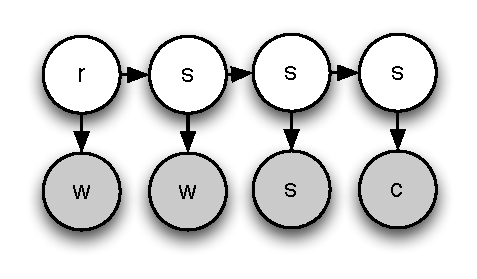
\includegraphics[scale=1]{figs/sequences/hmm}
\caption[HMM running example]{\label{fig:hmm} HMM structure, for the simple
running example.}
\end{figure}


A first order HMM model has the following independence assumptions over the joint distribution $\joint$:
\begin{itemize}
  \item \textbf{Independence of previous states.} The probability of
    being in a given state $\hv_l$ at position $\hs_i$ only depends on
    the state $\hv_m$ of the previous position $\hs_{i-1}$, that is 
    $p_{\theta} (\hs_i = \hv_l \mid \hs_{i-1} = \hv_m, \hs_{i-2} \ldots \hs_{1}) = p_{\theta} (\hs_i = \hv_l \mid \hs_{i-1} = \hv_m)$, 
    defining a first order Markov chain.%
    \footnote{The order of the Markov chain depends on the number of previous positions taken into account. 
    The remainder of the exposition can be easily extend to higher order HMM, giving the model more expressiveness, 
    but making inference harder.}
  \item \textbf{Homogeneous transition.} The probability of
    making a transition from state $\hv_l$ to state $\hv_m$ is independent of
    the particular position in the sentence, for all $i,j \in \{1,\ldots,N\}$:
    $p_{\theta} (\hs_i = \hv_l \mid \hs_{i-1} = \hv_m) =  p_{\theta}
    (\hs_j = \hv_l \mid \hs_{j-1} = \hv_m)$, so
    $p_{\theta} (\hs_i = \hv_l \mid \hs_{i-1} = \hv_m) = p_{\theta} (\hv_l \mid \hv_m)$.
  \item \textbf{Observation independence.}  The probability of
    observing $\vv_q$ at position $i$ is fully determined by the state
    at that position, that is  $p_{\theta}(\obs_i = \vv_q\mid
    \hs_i=\hv_l)$, and this probability is independent of the
    particular position, that is  $p_{\theta}(\obs_i = \vv_q\mid
    \hs_i=\hv_l)  = p_{\theta}(\vv_q\mid \hv_l)$.
\end{itemize}
These conditional independence assumptions are crucial to allow
efficient inference, as will be described. We also need to define a \emph{start probability}, the probability of starting 
at state $\hv_l$. Furthermore, when
dealing with text, it is usual to break the homogeneous transition
for the last position, and model the final transitions as 
independent parameters.
 The four probability
distributions that define the HMM model are summarized in Table
\ref{tab:hmm-dist}. 
For each one
of them we will use a short notation to simplify the exposition.
\begin{table}[h]
\begin{center}
\begin{tabular}{|l|l|l|}
\hline
\multicolumn{3}{|c|}{HMM distributions}\\
\hline
Name & probability distribution & short notation \\
\hline
\textbf{initial probability} & $p_{\theta} (\hs_1 = \hv_l)$ & $\pi_{l}$\\
\hline
\textbf{final probability} & $p_{\theta} (\hs_T = \hv_l \mid
\hs_{T-1} = \hv_m)$ & $f_{m,l}$\\
\hline
\textbf{transition probability} & $p_{\theta} (\hs_i = \hv_l \mid
\hs_{i-1} = \hv_m)$ & $a_{m,l}$\\
\hline
\textbf{observation probability} & $p_{\theta}(\obs_i = \vv_q\mid \hs_i = \hv_l)$ & $b_l(\obs_i) $ \\
\hline
\end{tabular}
\end{center}
\caption[HMM probability distributions]{\label{tab:hmm-dist} HMM probability distributions.}
\end{table}

The joint distribution can be expressed as:
\begin{equation}
  \joint =\pi_{\hs_1}b_{\hs_1}(\obs_1) [\prod_{i=2}^{N-1}
  a_{\hs_{i-1},\hs_{i}} b_{\hs_{i}}(\obs_i)] f_{\hs_{N-1},\hs_N}b_{\hs_{N}}(\obs_N),
  \label{eqn:hmm}
\end{equation}
which for the example from Figure \ref{fig:hmm} is:
\begin{equation}
  \joint =\pi_{r} b_r("w") a_{r,s}b_s("w") a_{s,s}b_s("s") f_{s,s}b_s("c").
  \label{eqn:hmm_ex}
\end{equation}

In the next section we turn our attention to estimating the different
probabilities distributions of the model  $\pi_l$, $a_{m,l}$,
$f_{m,l}$ and $b_l(\obs_i)$.

\begin{exercise}
Load the simple sequence dataset:
From the ipython command line (Note start ipython from the \emph{code}
directory), create a simple sequence object and look at the training
and test set.
\begin{python}
 In[]: run readers/simple_sequence.py
 In[]: simple = SimpleSequence()
 In[]: simple.train
Out[]: [w/r w/s s/s c/s , w/r w/r s/r c/s , w/s s/s s/s c/s ]
 In[]: simple.test
Out[]: [w/r w/s s/s c/s , c/s w/s t/s w/s ] 
\end{python}
\end{exercise}
%%% Local Variables: 
%%% mode: latex
%%% TeX-master: "../../guide"
%%% End: 






\section{\label{ml} Finding the Maximum Likelihood Parameters}
%So far we have not committed to any form for the probability
%distributions $\pi_l$, $a_{m,l}$ and $b_l(\obs_i)$. In both applications
%addressed in this class, both the observations and the hidden
%variables are discrete. The most common approach is to model each of
%these probability distributions as multinomial distributions,
%summarized in Table \ref{tt:mult-params}. Note that the number of parameters of $a_{l,m}$ is $|\hvocab|(|\hvocab|+1)$ because of the special ``STOP'' symbol.

%\begin{table}
%\begin{center}
%\begin{tabular}{|c|c|c|c|}
%\hline
%short notation & probability distribution  & |parameters|& constraint \\
%\hline
%$\pi_j$ & $p_{\theta} (\hs_1 = \hv_j)$ & $|\hvocab|$ & $\sum_{\hv \in \hvocab} \pi_j = 1$;\\
%\hline
%$a_{l,m}$ & $p_{\theta} (\hs_i = \hv_l \mid \hs_{i-1} = \hv_m)$ & $|\hvocab|(|\hvocab|+1)$ &$\sum_{\hv_l \in \hvocab} a_{m,l} = 1$;\\
%\hline
%%$f_{l,m}$ & $p_{\theta} (\hs_N = \hv_l \mid \hs_{N-1} = \hv_m)$ & $(|\hvocab|-1)^2$ &$\sum_{\hv_l \in \hvocab} t_{m,l} = 1$;\\
%%\hline
%$b_q(l) $& $p_{\theta}(\obs_i = \vv_q\mid \hs_i = \hv_l)$  & $|\hvocab||\vocab|$ &$\sum_{\vv_q \in \vocab} b_q(l)  = 1$.\\
%\hline
%\end{tabular}
%\end{center}
%\caption[HMM multinomial parametrization]{\label{tt:mult-params}Multinomial parametrization of the HMM distributions.}
%\end{table}

One important problem in HMMs is to estimate the 
model parameters, \emph{i.e.}, 
the distributions depicted in Table~\ref{tab:hmm-dist}. 
We will refer to the set of all these parameters 
as $\theta$. 
In a supervised setting, the HMM model
is trained to maximize the joint log-likelihood of the data. Given a
dataset $\mathcal{D}_L$, the objective being optimized is:
\begin{equation}
\argmax_{\theta} \sum_{m=1}^M \log P_{\theta}(X=x^m,Y=y^m),
\end{equation}
where $P_{\theta}(X=x^m,Y=y^m)$ is given by Eq.~\ref{eqn:hmm}.

In some applications (\emph{e.g.} speech recognition) 
the observation variables are continuous, hence the emission distributions are real-valued (\emph{e.g.} mixtures of Gaussians).
In our case, both the state set and the observation set are discrete (and finite), therefore we use
multinomial distributions for the emission and 
transition probabilities. 
Multinomial distributions are attractive for several reasons: first of
all, they are easy to implement; secondly, the maximum likelihood estimation of the parameters has a simple closed form. The parameters are just
normalized counts of events that occur in the corpus (the same as the
Na\"{i}ve Bayes from previous class).

Given our labeled corpus $\mathcal{D}_L$, the estimation process consists of counting how
many times each event occurs in the corpus and normalize the counts to
form proper probability distributions. Let us define the following
quantities, called sufficient statistics, that represent the counts of
each event in the corpus:

\begin{align}
\mathbf{Initial \ Counts\!:}\;\;\;\;  &  C_{\mathrm{init}}(c_k) = \sum_{m=1}^M
\Ind (y^m_1 = c_k); \label{eq::initialCounts}\\
%
%\mathbf{Final \ Counts\!:}\;\;\;\;  &  fc(\hv_l,\hv _m) = \sum_{\trex} 
%\Ind (\hs_N = \hv_l \mid \hs_{N-1} = \hv_m); \label{eq::finalCounts}\\
%
\mathbf{Transition \ Counts\!:}\;\;\;\;  &  C_{\mathrm{trans}}(c_k,c_l) =
\sum_{m=1}^M  \sum_{i = 2}^{N}
\Ind (y^m_i = c_k \wedge y^m_{i-1} = c_l); \label{eq::transitionCounts}\\
%
\mathbf{Final \ Counts\!:}\;\;\;\;  &  C_{\mathrm{final}}(c_k) = \sum_{m=1}^M
\Ind (y^m_N = c_k); \label{eq::finalCounts}\\
%
\mathbf{Emission \ Counts\!:}\;\;\;\;  &  
C_{\mathrm{emiss}}(w_j,c_k) = \sum_{m=1}^M
\sum_{i = 1}^{N}
\Ind (x^m_i = w_j \wedge y^m_i = c_k); \label{eq::emissionCounts}
\end{align}
Here $y^m_i$,  the underscript denotes the state index position for a given sequence, and the superscript denotes the sequence index in the dataset, and the same applies for the observations.
Note that $\Ind$ is an indicator function that has the value 1 when the
particular event happens, and zero otherwise. In other words, the previous
equations go through the training corpus and count how
often each event occurs. For example, Eq.~\ref{eq::transitionCounts} counts how many times $c_k$ follows state $c_l$. Therefore, $C_{\mathrm{trans}}(\text{\tt sunny},\text{\tt rainy})$ contains the number of times that a sunny day followed a rainy day.

%
%: e.g. the word ``w'' appears with state
%``s'', or state ``s'' follows another state ``s'', or state ``s''
%begins the sentence.


After computing the counts, one can perform some sanity checks
to make sure the implementation is correct. Summing over all entries
of each count table we should observe the following:

\begin{itemize}
\item \textbf{Initial \ Counts\!:} -- Should sum to the number of
  sentences: $\sum_{k=1}^K C_{\mathrm{init}}(c_k) = M$
%\item \textbf{Final \ Counts\!:} - Should sum to the number of sentences.
\item \textbf{Transition/Final \ Counts\!:} -- Should sum to the number of
  tokens: 
  $\sum_{k,l=1}^K C_{\mathrm{trans}}(c_k,c_l) + \sum_{k=1}^K C_{\mathrm{final}}(c_k) = MN$
%   minus 2 times the number of sentences. Note that there are
%  N-1 edges for each sentence, and the last edge is being accounted by
%  the final transitions. So this leaves us with N-2 edges per sentence,
%  where N is the number of tokens in that sentence.
\item \textbf{Observation \ Counts\!:} -- Should sum to the number of tokens: $\sum_{j=1}^J\sum_{k=1}^K C_{\mathrm{emiss}}(w_j,c_k) = MN$.
\end{itemize}

Using the sufficient statistics (counts) the parameter estimates are: 
\begin{align}
  P_{\mathrm{init}}(c_k | \text{\tt start}) &=  \frac{C_{\mathrm{init}}(c_k)}{\sum_{l=1}^K
    C_{\mathrm{init}}(c_l)}\\
  P_{\mathrm{final}}(\text{\tt stop} | c_l) &=  \frac{C_{\mathrm{final}}(c_l)}{\sum_{k=1}^K
    C_{\mathrm{trans}}(c_k,c_l) + C_{\mathrm{final}}(c_l)}\\
  P_{\mathrm{trans}}(c_k | c_l) &=  \frac{C_{\mathrm{trans}}(c_k,c_l)}{\sum_{p=1}^K
    C_{\mathrm{trans}}(c_p,c_l) + C_{\mathrm{final}}(c_l)}\\
  P_{\mathrm{emiss}}(w_j | c_k) &=  \frac{C_{\mathrm{emiss}}(w_j,c_k)}{\sum_{q=1}^J
    C_{\mathrm{emiss}}(w_q,c_k)}
\end{align}


%\begin{exercise}
%Convince yourself that the sanity checks described above are true.
%Collect the counts from a supervised corpus using method
%\emph{collect\_counts\_from\_corpus} and use the provided function \emph{sanity\_check\_counts} to perform these checks on the counts table. 
%%\begin{python}
%% def sanity_check_counts(self,seq_list):
%%\end{python}
%
%\begin{python}
%>>> import sequences.hmm as hmmc
%>>> hmm = hmmc.HMM(simple.x_dict, simple.y_dict)
%>>> hmm.train_supervised(simple.train)
%>>> hmm.sanity_check_counts(simple.train)
%>>> print "Initial Probabilities:", hmm.initial_probs
%
%>>> print "Transition Probabilities:", hmm.transition_probs
%
%>>> print "Final Probabilities:", print 
%hmm.final_probs
%
%>>> print "Emission Probabilities", print hmm.emission_probs
%
%Initial counts match
%Final counts match
%Transition counts match
%Observations counts match
%\end{python}
%\end{exercise}



\begin{exercise}
The provided function \emph{train\_supervised} from the \emph{hmm.py} file implements the above parameter estimates.
%Implement a function that estimates the maximum likelihood
%estimates for the parameters given the corpus in the class HMM.
%The function header is in the hmm.py file. 
%\begin{python}
%def train_supervised(self,sequence_list):
%\end{python}
Run this function given the simple dataset above and look at the estimated probabilities. Are they correct? You can also check the variables ending in \emph{\_counts} instead of \emph{\_probs} to see the raw counts (for example, typing \emph{hmm.initial\_counts} will show you the raw counts of initial states). How are the counts related to the probabilities?

\begin{python}
>>> import lxmls.sequences.hmm as hmmc
>>> hmm = hmmc.HMM(simple.x_dict, simple.y_dict)
>>> hmm.train_supervised(simple.train)
>>> print "Initial Probabilities:", hmm.initial_probs
[ 0.66666667  0.33333333]
>>> print "Transition Probabilities:", hmm.transition_probs
[[ 0.5    0.   ]
 [ 0.5    0.625]]
>>> print "Final Probabilities:", hmm.final_probs
[ 0.     0.375]
>>> print "Emission Probabilities", hmm.emission_probs
[[ 0.75   0.25 ]
 [ 0.25   0.375]
 [ 0.     0.375]
 [ 0.     0.   ]]
\end{python}
\end{exercise}


%%% Local Variables: 
%%% mode: latex
%%% TeX-master: "../../guide"
%%% End: 




\section{\label{decoding} Decoding a Sequence}
Given the learned parameters and a new
observation sequence $x = x_1\ldots x_N$, we want to find the sequence of hidden states $y^* = y_1^* \ldots y_N^*$ that ``best'' explains it.
 This is called the \emph{decoding} problem. There are several ways to define what we mean by the ``best''
$y^*$, depending on our goal: for instance, we may want to minimize the probability of error
on each hidden
variable $Y_i$, or we may want to find the best assignment
to the sequence $Y_1\ldots Y_N$ as a whole. 
Therefore, finding the best sequence
can be accomplished through different approaches:

\begin{itemize}
\item A first approach, normally called \textbf{posterior decoding} or \textbf{minimum risk decoding}, consists
in picking the highest state posterior for each position $i$ in the sequence:
\begin{equation}
y_i^* = \argmax_{y_i \in \Lambda} P(Y_i=y_i | X_1=x_1,\ldots,X_N =x_N).
\end{equation}
%where $\gamma_i(\hs_i)$ is the posterior probability $P(\hs_i|\sent)$. 
Note, however, that this approach does not guarantee that the sequence $y^*=y_1^* \ldots y_N^*$ will be a
valid sequence of the model. For instance, there might be a transition
between two of the best state posteriors with probability zero. 

\item A second approach, called \textbf{Viterbi decoding}, consists in
picking the best global hidden state sequence: 
\begin{eqnarray}
y^* &=& \argmax_{y = y_1\ldots y_N} P(Y_1=y_1,\ldots, Y_N=y_N | X_1=x_1,\ldots,X_N =x_N)\nonumber\\
&=& \argmax_{y = y_1\ldots y_N} P(Y_1=y_1,\ldots, Y_N=y_N, X_1=x_1,\ldots,X_N =x_N).
\end{eqnarray}
\end{itemize}

Both approaches (which will be explained in Sections~\ref{posterior} and~\ref{viterbi}, respectively) rely on dynamic programming and make use of the
independence assumptions of the HMM model. Moreover, they use an alternative
representation of the HMM called a \emph{trellis}. 

A trellis unfolds all possible states for each position and it makes explicit the independence assumption: each position only
depends on the previous position. Here, each column represents a position in the sequence and each row represents a possible state. Figure \ref{fig:trellis} shows the
trellis for the particular example in Figure \ref{fig:hmm}. 

\begin{figure}[ht]
\centering
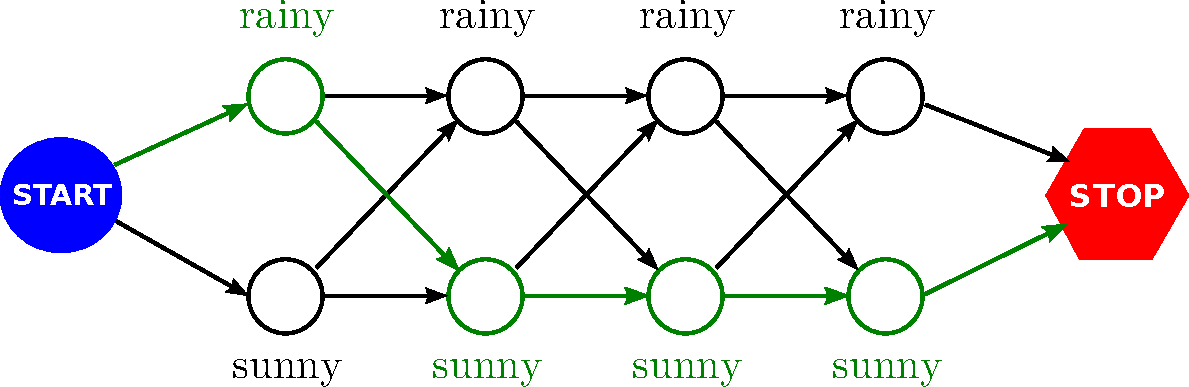
\includegraphics[width=0.7\textwidth]{figs/sequences/trellis_new}
\caption[HMM Trellis representation.]{\label{fig:trellis} Trellis
  representation of the HMM in Figure ~\ref{fig:hmm}, for the observation
  sequence ``{\tt walk} {\tt walk} {\tt shop} {\tt clean}'', where each hidden variable can take the values {\tt rainy} or {\tt sunny}.}
\end{figure}




Considering the trellis representation, note that we can include the following information:
\begin{itemize}
\item an \emph{initial probability} to the arrows that depart from the start symbol;
\item a \emph{final probability} to the arrows that reach the stop symbol;
\item a \emph{transition probability} to the remaining arrows; and,
\item an \emph{emission probability} to each circle, which is the probability that the observed symbol is emitted by that particular state.
\end{itemize}

For convenience, we will be working with 
log-probabilities, rather than probabilities.\footnote{This will be motivated further in Section~\ref{sec:logdomain}, where we describe 
how operations can be performed efficiently
in the log-domain.} Therefore, if we associate to each circle and arrow in
the trellis a score that corresponds
to the log-probabilities above, 
and if we define the score of a path
connecting the {\tt start} and  {\tt stop} symbols as
the sum of the scores of the circles and arrows
it traverses, 
then 
the goal of finding the most likely sequence of states (Viterbi decoding) corresponds to 
finding the path with the highest score.




%---since 
%we'll be multiplying a lot of probabilities, 
%we prevent underflowing by working in the log-domain. 

%For the decoding algorithms described in the following sections, 
%it is
%useful to define a re-parametrization of the model in equation \eqref{eqn:hmm}, in terms of
%node potentials $\phi_n(l)$ (associating a number to each box in Figure \ref{fig:trellis})
%and edge potentials $\phi_{n-1,n}(l,m)$ (associating a number to each edge in  Figure
%\ref{fig:trellis}). For our example, this re-parametrization is given by
%%
%\begin{equation}
%  \joint =\phi_1(r)\phi_1(r,s)\phi_2(s)\phi_2(s,s)\phi_3(s)\phi_3(s,s)\phi_4(s).
%  \label{eqn:hmm_ex_treelis}
%\end{equation}
%
%%\begin{equation}
%%  \joint =\phi_1(``w'',r)\phi_1(r,s)\phi_2(``w'',s)\phi_2(s,s)\phi_3(``s'',s)\phi_3(s,s)\phi_4(``c'',s).
%%  \label{eqn:hmm_ex_treelis}
%%\end{equation}
%
%In other words, to do this re-parameterization we need to find expressions for the potential variables, (the $\phi$'s) such that \eqref{eqn:hmm} and \eqref{eqn:hmm_ex_treelis} are equal. The solution is given by
%\begin{equation}
%\phi_{i-1,i}(l,m) = a_{l,m}
%\label{eq:nodes1}
%\end{equation}
%and
%\begin{equation}
%\phi_i(l) = 
%\begin{cases}
% b_{\obs_i}(l)\pi_l \quad\text{i = 1}\\
% b_{\obs_i}(l) \quad\text{i = 2,\ldots,N-1}\\
% b_{\obs_i}(l)a_{l,STOP} \quad\text{i = N}
% \label{eq:nodes2}
%\end{cases}
%\end{equation}


%\begin{itemize}
%\item\emph{Edge Potentials} - correspond to the transition parameters, with the exception of the
%edges into the last position that correspond to the final transition parameters.
%\item\emph{Node Potentials} - correspond to the observation
%parameters for a given state and the observation at that position.  The
%first position is the exception and corresponds to the
%product between the observation parameters for that state and
%the observation in that position with the initial parameters for that state. 
%\end{itemize}

%Although this re-parametrization simplifies the exposition, and will be
%used in these lectures, it is not necessarily very practical since we
%will be reproducing several values (for instance the transition
%parameters for each position).


The trellis scores are given by the following expressions:
\begin{itemize}
\item For each state $c_k$:
\begin{eqnarray}
\mathrm{score}_{\mathrm{init}}(c_k) &=&
\log P_{\mathrm{init}}(Y_{1} = c_k | \text{\tt start}).
\end{eqnarray}
\item For each position $i \in {1,\ldots,N-1}$ and each pair of states $c_k$ and $c_l$:
\begin{eqnarray}
\mathrm{score}_{\mathrm{trans}}(i, c_k, c_l) &=&
\log P_{\mathrm{trans}}(Y_{i+1} = c_k | Y_i = c_l).
\end{eqnarray}
\item For each state $c_l$:
\begin{eqnarray}
\mathrm{score}_{\mathrm{final}}(c_l) &=&
\log P_{\mathrm{final}}(\text{\tt stop} | Y_N = c_l).
\end{eqnarray}
\item For each position $i \in {1,\ldots,N}$ and state $c_k$:
\begin{eqnarray}
\mathrm{score}_{\mathrm{emiss}}(i, c_k) &=&
\log P_{\mathrm{emiss}}(X_i = x_i | Y_i = c_k).
\end{eqnarray}
\end{itemize}

In the next exercise, you will compute the trellis scores.

\begin{exercise}
Convince yourself that the score of a path in the trellis 
(summing over the scores above) is equivalent 
to the log-probability $\log P(X=x,Y=y)$, 
as defined in 
Eq.~\ref{eqn:hmm_ex}. 
Use the given function \emph{compute\_scores} on the first training sequence and confirm that the values are correct. You should get the same values as presented below.

%Implement a function that builds the node and edge potentials for a
%given sequence. The function head is in the \emph{hmm.py} file:

%\begin{python}
% def build_potentials(self,sequence):
%\end{python}
%
%Run this function for the first training sequence from the simple
%dataset and compare the results given (If the results are the same
%then you are ready to go).

\begin{python}
initial_scores, transition_scores, final_scores, emission_scores = hmm.compute_scores(simple.train.seq_list[0])
print initial_scores

[-0.40546511 -1.09861229]

print transition_scores

[[[-0.69314718        -inf]
  [-0.69314718 -0.47000363]]

 [[-0.69314718        -inf]
  [-0.69314718 -0.47000363]]

 [[-0.69314718        -inf]
  [-0.69314718 -0.47000363]]]

print final_scores

[       -inf -0.98082925]

print emission_scores

[[-0.28768207 -1.38629436]
 [-0.28768207 -1.38629436]
 [-1.38629436 -0.98082925]
 [       -inf -0.98082925]] 
\end{python}

Note that scores which are $-\infty$ (\texttt{-inf}) correspond
to zero-probability events. 
\end{exercise}

\subsection{Computing in log-domain}\label{sec:logdomain}

We will see that the decoding algorithms 
will need to multiply twice as many probability terms as 
the length $N$ of the sequence. 
This may cause underflowing problems 
when $N$ is large, since the nested multiplication of numbers smaller than 1
may easily become smaller than the machine precision. To avoid that
problem, \cite{rabiner} presents a scaled version of the decoding algorithms that avoids this problem.
An alternative, which is widely used, is computing
in the log-domain. That is, instead of 
manipulating probabilities, manipulate log-probabilities (the scores presented above). 
Every time we need to multiply probabilities, 
we can sum their log-representations, since:
\begin{equation}
\log(\exp(a) \times \exp(b)) = a+b.
\end{equation}
Sometimes, we need to \emph{add} probabilities. 
In the log domain, this requires us to compute 
\begin{equation}
\log(\exp(a) + \exp(b)) = a + \log(1 + \exp(b-a)),
\end{equation}
where we assume that $a$ is smaller than $b$.


\begin{exercise}
Look at the module {\tt sequences/log\_domain.py}. 
This module implements a function
{\tt logsum\_pair(logx, logy)} to 
add two numbers represented in the log-domain;
it returns their sum also represented in the log-domain. The function {\tt logsum(logv)} 
sums all components of an array 
represented in the log-domain. 
This will be used later in our decoding algorithms.
To observe why this is important, type the 
following:
\begin{python}
import numpy as np
a = np.random.rand(10)
np.log(sum(np.exp(a)))
2.8397172643228661

np.log(sum(np.exp(10*a)))
10.121099917705818

np.log(sum(np.exp(100*a)))
93.159220940569128

np.log(sum(np.exp(1000*a)))
inf

from lxmls.sequences.log_domain import *
logsum(a)
2.8397172643228665

logsum(10*a)
10.121099917705818

logsum(100*a)
93.159220940569114

logsum(1000*a)
925.88496219586864
\end{python}
\end{exercise}


\subsection{Posterior Decoding}\label{posterior}
Posterior decoding consists
in picking state with the highest posterior for each position in the sequence independently; for 
each $i = 1,\ldots,N$:
\begin{equation}
y_i^* = \argmax_{y_i \in \statevocab} P(Y_i=y_i | X = x).
\end{equation}
The \textbf{sequence posterior distribution} is the probability of a particular
hidden state sequence given that we have observed a particular
sequence. Moreover, we will be interested in two other posteriors distributions:
the \textbf{state posterior distribution}, corresponding to the
probability of being in a given state in a certain position given the
observed sequence; and the \textbf{transition posterior distribution},
which is the probability of making a particular transition, from position $i$ to
$i+1$, given the observed sequence. They are formally defined as follows:
\begin{align}
  \mathbf{Sequence \ Posterior\!:}\;\;\;\; &P(Y=y|X=x) = \frac{P(X=x,Y=y)}{P(X=x)}; \label{eq::posteriorDistribution} \\
 \mathbf{State \ Posterior\!:}\;\;\;\;  & P(Y_i=y_i | X=x); \label{eq::nodePosterior} \\
 \mathbf{Transition \ Posterior\!:}\;\;\;\;  &P(Y_{i+1}=y_{i+1},Y_i=y_i| X=x).\label{eq::edgePosterior}
\end{align}

To compute the posteriors, a first step is to be able to compute the 
likelihood of
the sequence $P(X=x)$, which corresponds to summing the probability of all
possible hidden state sequences.
\begin{equation}
\label{likelihoood}
\mathbf{Likelihood\!:}\;\;\;\; P(X=x) = \displaystyle \sum_{y \in \statevocab^N} P(X=x,Y=y).
\end{equation}
The number of possible hidden state sequences is exponential in the
length of the sequence ($|\statevocab|^N$),
 which makes the sum over all of them hard. 
 In our simple
 example, there are $2^4 = 16$ paths, which we can actually explicitly enumerate
 and calculate their probability using Equation \ref{eqn:hmm}. But this is as far as it goes: for example, for Part-of-Speech
 tagging with a small tagset of 12 tags and a medium size
 sentence of length 10, there are $12^{10} = 61 917 364 224$ such
 paths. 
Yet, we must be able to compute this sum (sum over $y \in \statevocab^N$) to compute the above likelihood
formula; this is called the inference problem. For sequence models, there is a well known dynamic programming algorithm,
the \textbf{Forward-Backward} (FB) algorithm, which allows the computation
to be performed in linear time,%
\footnote{The runtime is linear with respect
to the sequence length. More precisely, 
the runtime is $O(N|\statevocab|^2)$. 
A naive enumeration would cost $O(|\statevocab|^N)$.} %
by making use of the independence assumptions.

The FB algorithm relies on the independence of previous states
assumption, which  
is illustrated in the trellis view by having arrows only between consecutive states. 
The FB algorithm defines two auxiliary probabilities, the forward probability and the backward probability. 

\subsection*{Efficient forward probability computation}
The forward probability represents the probability that in position
$i$ we are in state $Y_i = c_k$ and that we have observed $x_1,\ldots,x_i$
up to that position. Therefore, its mathematical expression is:
\begin{equation}
\label{eq::forward}
\mathbf{Forward \ Probability\!:}\;\;\;\;  \mathrm{forward}(i, c_k) = P(Y_i = c_k, X_1=x_1,\ldots, X_i = x_i)
\end{equation}

Using the independence assumptions of the HMM we can compute $\mathrm{forward}(i, c_k)$ using all the forward computations \{$\mathrm{forward}(i -1, c)$ for $c \in \statevocab$\}. In order to facilitate the notation of the following argument we will denote by $x_{i:j}$  the assignemnt $X_i = x_i, \dots, X_j = x_j$. Therefore we can write   $\mathrm{forward}(i, y_i) $ as $P( y_i, x_{1:i } ) $ and rewrite the forward expression as follows:
\begin{equation}
\label{eq::forward2}
  P( y_i, x_{1:i } ) =  \sum_{y_{i-1} \in \statevocab} P( y_i ,y_{i-1}, x_{1:i } )  =  \sum_{y_{i-1} \in \statevocab} P( x_i  | y_i,  y_{i-1},  x_{1:i-1 } ) \cdot P(y_i  | y_{i-1},  x_{1:i-1 }) \cdot P(y_{i-1},  x_{1:i-1 })  
\end{equation}

Using the \textbf{Observation independence} and the \textbf{Independence of previous states} properties of the first order HMM we have $P( x_i  | y_i,  y_{i-1},  x_{1:i-1 } ) = P( x_i  | y_i) $ and $P(y_i  | y_{i-1},  x_{1:i-1 })  = P(y_i  | y_{i-1})  $. Therefore equation (\ref{eq::forward2}) can be written, 
for $i \in \{2,\dots,N\}$ (where $N$ is the length of the sequence), as 
\begin{equation}
\label{eq::forward3}
 \mathrm{forward}(i, y_i)  = \sum_{y_{i-1} \in \statevocab} P( x_i  | y_i, ) \cdot P(y_i  | y_{i-1}) \cdot \mathrm{forward}(i-1, y_{i-1})   
\end{equation}

 Using equation (\ref{eq::forward3}) we have proved that  the forward probability can be defined by the
following recurrence rule: 
\begin{eqnarray}
\mathrm{forward}(1, c_k)&=& P_{\mathrm{init}}(c_k|\text{\tt start}) \times 
P_{\mathrm{emiss}}(x_1 | c_k)
 \\
 \mathrm{forward}(i, c_k) &=& \left( \displaystyle \sum_{c_l \in \statevocab} P_{\mathrm{trans}}(c_k | c_l) \times \mathrm{forward}(i-1, c_l) \right) \times P_{\mathrm{emiss}}(x_i | c_k)  \label{forwardRecursion}
 \\
  \mathrm{forward}(N+1, \text{\tt stop}) &=& \sum_{c_l \in \statevocab} P_{\mathrm{final}}(\text{\tt stop} | c_l) \times \mathrm{forward}(N, c_l).
\end{eqnarray}

%\begin{figure}
%\begin{center}
%\begin{tabular}{cc}
%
%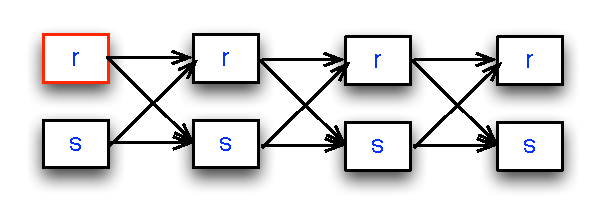
\includegraphics[scale=.5]{figs/sequences/forward1}
%& 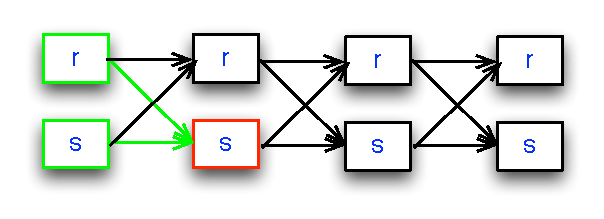
\includegraphics[scale=.5]{figs/sequences/forward2}\\
%\end{tabular}
%\caption[Forward-backward example.]{\label{fig:fb} Forward trellis for
%  the first sentence of the training data at position 1 (left) and at
%  position 2 (right)}
%
%\end{center}
%\end{figure}

%At position 1, the probability of being in state ``r'' and observing word ``w'' is just the node
%marginal for that position: $\alpha_1(r) = \phi_1(r)$ (see Figure
% \ref{fig:fb} left). At position 2 the probability
%of being in state ``s'' and observing the sequence of words ``w w''
%corresponds to the sum of all possible ways of reaching position 2 in
%state ``s'', namely, ``rs'' and ``ss'' (see Figure \ref{fig:fb} right). The probability of the former is
%$\phi_1(r)\phi_1(r,s)\phi_2(s)$
%and that of the latter is $\phi_1(s)\phi_1(s,s)\phi_2(s)$, so we get:
%\begin{eqnarray*}
%   \alpha_2(s) &=& \phi_1(r)\phi_1(r,s)\phi_2(s) +
%   \phi_1(s)\phi_1(s,s)\phi_2(s) \\
%   \alpha_2(s) &=& \left[\phi_1(r)\phi_1(r,s) +
%   \phi_1(s)\phi_1(s,s) \right]\phi_2(s) \\
% \alpha_2(s) &=& \displaystyle \sum_{\hs \in \hvocab}
% \left[\phi_1(\hs)\phi_1(\hs,s)\phi_2(s) \right] \\
%  \alpha_2(s) &=& \displaystyle \sum_{\hs \in \hvocab}
% \left[\alpha_1(\hs)\phi_1(\hs,s)\phi_2(s) \right]
%\end{eqnarray*}

Using the forward trellis one can compute the likelihood simply as:
\begin{equation}
\label{eq:forwardSum}
P(X=x) = \mathrm{forward}(N+1, \text{\tt stop}).
\end{equation}

Although the forward probability is enough to calculate the likelihood of a given sequence, we will also need the backward probability to calculate the state posteriors. 

% We could include a graph and comment the d-separation property which implies the conditional independence assumptions of the HMM graphically.
%\begin{figure}[ht]
%\centering
%\includegraphics[width=0.5\textwidth]{figs/sequences/hmm_diagram}
%\caption[HMM diagram]{\label{fig:hmm_diagram}Diagram showing the conditional independence relations of the HMM. If $Y_i$ is observed then...}
%\end{figure}

\subsection*{Efficient backward probability computation}

The backward probability is similar to the forward probability, but operates in the inverse direction.
It represents the probability of observing $x_{i+1},\ldots,x_N$ from position $i+1$ up to $N$, given that at position $i$ we are at state $Y_i = c_l$:
 \begin{equation}
\label{eq::backward}
\mathbf{Backward \ Probability\!:}\;\;\;\;  \mathrm{backward}(i, c_l) = P(X_{i+1}=x_{i+1},\ldots, X_N=x_N | Y_i = c_l).
\end{equation}

Using the independence assumptions of the HMM we can compute $\mathrm{backward}(i, c_k)$ using all the backward computations \{$\mathrm{backward}(i +1, c)$ for $c \in \statevocab$\}. Therefore we can write   $\mathrm{backward}(i, y_i) $ as $P( x_{i+1:N} | y_i ) $ and rewrite the forward expression as follows:
\begin{equation}
\label{eq::backward2}
  P( x_{i+1:N} | y_i ) =  \sum_{y_{i+1} \in \statevocab} P( x_{i+1:N}, y_{i+1} | y_i)  =  \sum_{y_{i+1} \in \statevocab} P( x_{i+2:N} | y_i, y_{i+1}, x_{i+1}) 
   P( x_{i+1}, |  y_{i+1},  y_{i}) P( y_{i+1} | y_i)
\end{equation}

Using the previous equation we have proved that the backward probability can be defined by the following recurrence rule:

\begin{eqnarray}
\mathrm{backward}(N, c_l) &=& P_{\mathrm{final}}(\text{\tt stop} | c_l) 
 \\
 \mathrm{backward}(i, c_l) &=&  \displaystyle \sum_{c_k \in \statevocab} P_{\mathrm{trans}}(c_k | c_l) \times \mathrm{backward}(i+1, c_k) \times P_{\mathrm{emiss}}(x_{i+1} | c_k)  \label{backwardRecursion}
 \\
  \mathrm{backward}(0, \text{\tt start}) &=& \sum_{c_k \in \statevocab} P_{\mathrm{init}}(c_k | \text{\tt start}) \times \mathrm{backward}(1, c_k) \times P_{\mathrm{emiss}}(x_{1} | c_k).
\end{eqnarray}
%At position $N$ there are no more observations, and the backward
%probability is set to 1. At position $i$, the probability 
%of having observed the future and being in state $\hv_l$, is given by the sum for all possible states of the probability of having transitioned 
%from position $i$ with state $\hv_l$ to position $i+1$ with state $\hv_m$, and observing $\obs_{i+1}$ at time $i+1$ and the future from there onward, which is $\beta_{i+1}(\hs_{i+1} = \hv_m)$. 
Using the backward trellis one can compute the likelihood simply as:.
\begin{equation}
\label{eq:backwardSum}
P(X=x) = \mathrm{backward}(0, \text{\tt start}).
\end{equation}

\subsection*{The forward backward algorithm}

We have seen how we can compute the probability of a sequence $x$ using the the forward and backward probabilities by computing  $\mathrm{forward}(N+1, \text{\tt stop})$ and $ \mathrm{backward}(0, \text{\tt start})$ respectively. Moreover,  the probability of a sequence $x$ can be computed with both forward and backward probabilities at a particular position $i$. The probability of a  given sequence $x$ at any position $i$ in the sequence can be computed
as follows \footnote{ The second equality in \ref{eq::fbsanity} can be justified as follows. Since $Y_i=y_i$ is observed then  $X_{i+1}, \dots, X_{N}$ is conditionally independent from any $X_k$ for $k \leq i$ . Therefore  $P(x_1,\dots, x_N, y_i) =  P( x_{i+1},\dots, x_N �| yi , x_1, \dots,x_i ) \cdot P( yi , x_1, \dots,x_i ) =  P( x_{i+1},\dots, x_N �| yi  ) \cdot P( yi , x_1, \dots,x_i ) = backward(i,y_i) \cdot forward(i,y_i)$.}:


\begin{eqnarray}
\label{eq::fbsanity}
  P(X=x) &=& 
  \sum_{c_k \in \statevocab} P(X_1=x_1,\ldots, X_N=x_N,Y_i=c_k)\nonumber\\
  & =&
  \sum_{c_k \in \statevocab} 
  \underbrace{P(X_1=x_1,\ldots, X_i=x_i, Y_i=c_k)}_{\mathrm{forward}(i,c_k)} \times 
  \underbrace{P(X_{i+1}=x_{i+1},\ldots, X_N=x_N| Y_i=c_k)}_{\mathrm{backward}(i,c_k)}\nonumber\\
  &=& \sum_{c_k \in \statevocab} \mathrm{forward}(i,c_k) \times \mathrm{backward}(i,c_k).
\end{eqnarray}


This equation will work for any choice of $i$. Although redundant, this fact is useful when implementing an
HMM as a sanity check that the computations are being performed
correctly, since one can compute this expression for several $i$; they should all yield the same value. 

Algorithm \ref{alg:fb} shows the pseudo code for the forward backward algorithm. The reader can notice that the $forward$ and $backward$ computations in the algorithm make use of $P_{emiss}$ and $P_{trans}$. There are a couple of details that should be taken into account if the reader wants to understand the algorithm using scores instead of probabilities.

% maybe more details on how to implement the algorithm using "scores" instead of probabilities should be given. 
\begin{itemize}
\item  $forward(i,\hat{c})$  is computed using $P_{emiss}(x_i | \hat{c})$ which does not depend on the sum over all possible states $c_k \in  \statevocab $. Therefore when taking the logarithm of the sum over all possible states the recurrence of the forward computations can be split as a sum of two logarithms.
\item $backward(i,\hat{c})$  is computed using $ P_{\mathrm{trans}}(c_k | \hat{c} )$ and $P_{\mathrm{emiss}}(x_{i+1} | c_k) $ both of  which  depend on $c_k$. Therefore when taking the logarithm of the sum the expression cannot be split as a sum of logarithms.
\end{itemize}


\begin{algorithm}[t]
   \caption{Forward-Backward algorithm \label{alg:fb}}
\begin{algorithmic}[1]
   \STATE {\bfseries input:} sequence $x_1,\ldots,x_N$, scores $P_{\mathrm{init}}, P_{\mathrm{trans}}, P_{\mathrm{final}}, P_{\mathrm{emiss}}$
        \item[]
        \STATE  \emph{Forward pass}: Compute the forward probabilities
        %\STATE \emph{Initialization}
        \FOR{$c_k \in \statevocab$ }
        \STATE $\mathrm{forward}(1,c_k) = P_{\mathrm{init}}(c_k|\text{\tt start}) \times 
P_{\mathrm{emiss}}(x_1 | c_k)$
        \ENDFOR 
        \FOR{$i=2$ {\bfseries to} $N$}
         \FOR{$\hat{c} \in \statevocab$ }
                 \STATE $\mathrm{forward}(i, \hat{c} ) = \left( \displaystyle \sum_{c_k \in \statevocab} P_{\mathrm{trans}}(\hat{c}| c_k) \times \mathrm{forward}(i-1, c_k) \right) \times P_{\mathrm{emiss}}(x_i | \hat{c})$
         \ENDFOR 
        \ENDFOR 
       \item[]
       \STATE \emph{Backward pass}: Compute the backward probabilities
      % \STATE \emph{Initialization}
        \FOR{$c_k \in \statevocab$ }
        \STATE $\mathrm{backward}(N, c_k) = P_{\mathrm{final}}(\text{\tt stop} | c_k)$
        \ENDFOR 
       \FOR{$i=N-1$ {\bfseries to} 1}
                 \FOR{$\hat{c} \in \statevocab$ }
       \STATE $\mathrm{backward}(i, \hat{c}) =  \displaystyle \sum_{c_k \in \statevocab} P_{\mathrm{trans}}(c_k | \hat{c} ) \times \mathrm{backward}(i+1, c_k) \times P_{\mathrm{emiss}}(x_{i+1} | c_k)$
       	 \ENDFOR 
        \ENDFOR 
        \item[]
       \STATE \textbf{output:} The forward and backward probabilities.
\end{algorithmic}
\end{algorithm}




\begin{exercise}
%Given the implementation of the forward pass of the forward backward
%algorithm in the file \emph{forward\_backward.py}, implement the backward pass.
%\begin{python}
%
%def forward_backward(node_potentials,edge_potentials):
%    H,N = node_potentials.shape
%    forward = np.zeros([H,N],dtype=float)
%    backward = np.zeros([H,N],dtype=float)
%    forward[:,0] = node_potentials[:,0]
%    ## Forward loop
%    for pos in xrange(1,N):
%        for current_state in xrange(H):
%            for prev_state in xrange(H):
%                forward_v = forward[prev_state,pos-1]
%                trans_v = edge_potentials[prev_state,current_state,pos-1]
%                prob = forward_v*trans_v
%                forward[current_state,pos] += prob
%            forward[current_state,pos] *= node_potentials[current_state,pos]
%    ## Backward loop
%          ## Your code
%   return forward,backward
%
%\end{python}

Run the provided forward-backward algorithm on the first train sequence. 
Observe that both the forward and the backward 
passes give the same log-likelihood.
%Use the provided function that makes use of Equation \ref{eq::fbsanity} to make
%sure your implementation is correct: 
\begin{python}
log_likelihood, forward = hmm.decoder.run_forward(initial_scores, transition_scores, final_scores, emission_scores)
print 'Log-Likelihood =', log_likelihood

Log-Likelihood = -5.06823232601

log_likelihood, backward = hmm.decoder.run_backward(initial_scores, transition_scores, final_scores, emission_scores)
print 'Log-Likelihood =', log_likelihood

Log-Likelihood = -5.06823232601
\end{python}
\end{exercise}


Given the forward and backward probabilities, one can compute both the state
and transition posteriors 
(you can hint why by looking at the term inside the sum in Eq.~\ref{eq::fbsanity}).


\begin{align}
 \mathbf{State \ Posterior\!:}\;\;\;\;  & P(Y_i = y_i| X=x) = \frac{\mathrm{forward}(i, y_i) \times 
 \mathrm{backward}(i, y_i)}{P(X=x)}; \label{eq::nodePosterior2} \\
 \mathbf{Transition \ Posterior\!:}\;\;\;\; &
 P(Y_i = y_i, Y_{i+1} = y_{i+1} | X=x)= \nonumber\\
 &
   \frac{\mathrm{forward}(i, y_i) \times 
   P_{\mathrm{trans}}(y_{i+1}|y_i) \times
   P_{\mathrm{emiss}}(x_{i+1}|y_{i+1}) \times
 \mathrm{backward}(i+1, y_{i+1})}{P(X=x)}.\label{eq::edgePosterior2}
\end{align}

A graphical representation of these posteriors is illustrated in Figure~\ref{fig:posteriors}. 
On the left it is shown that $\mathrm{forward}(i, y_i)  \times \mathrm{backward}(i, y_i)$ returns the sum of all paths that contain the state $y_i$, weighted by $P(X=x)$; on the right we can see that $\mathrm{forward}(i, y_i) \times P_{\mathrm{trans}}(y_{i+1}|y_i) \times P_{\mathrm{emiss}}(x_{i+1}|y_{i+1}) \times \mathrm{backward}(i+1, y_{i+1})$  returns the same for all paths containing the edge from $y_i$ to $y_{i+1}$.
%Thus, these posteriors can be seen as the ratio of the number of paths that contain the given state or transition (weighted by $P(X=x)$) and the number of possible paths in the graph $\marginal$.

As a practical example, given that the person performs the sequence of actions ``{\tt walk} {\tt walk} {\tt shop} {\tt clean}", we want to know the probability of having been raining in the second day. The state posterior probability for this event can be seen as the probability that the sequence of actions above was generated by a sequence of weathers and where it was raining in the second day. In this case, the possible sequences would be all the sequences which have {\tt rainy} in the second position.

\begin{figure}
\begin{center}
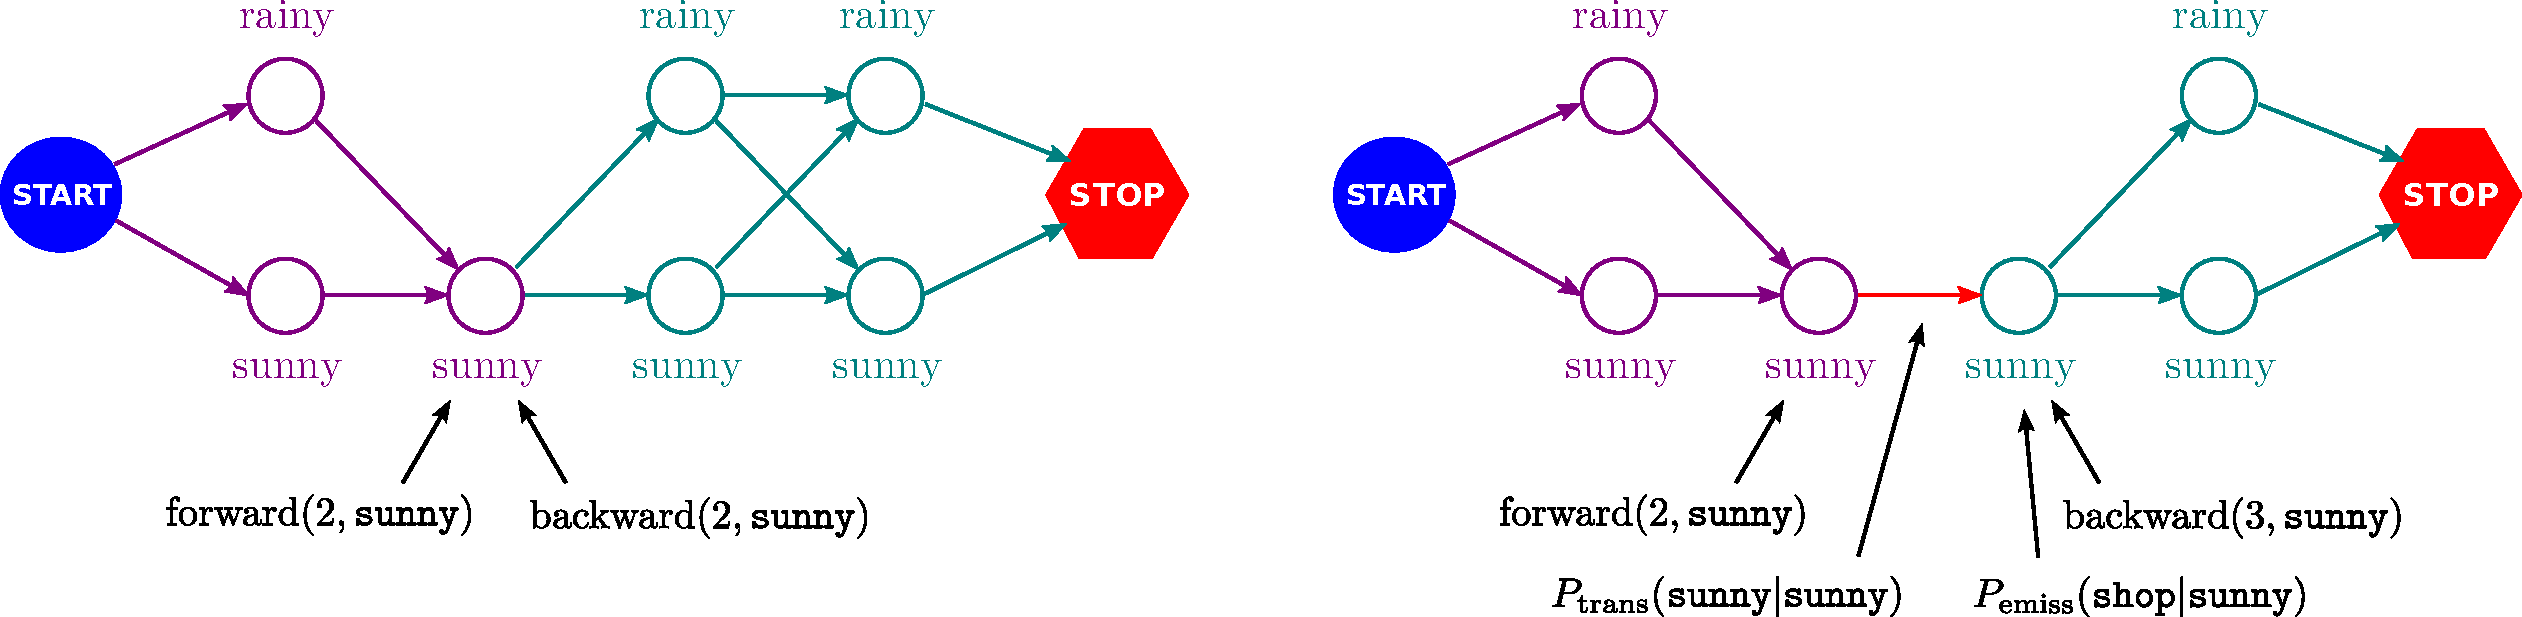
\includegraphics[width=1\textwidth]{figs/sequences/posteriors}
\caption[Posterior Illustration.]{\label{fig:posteriors} A graphical representation of the components in the state and transition posteriors. Recall that the observation sequence is ``\texttt{walk walk shop clean}''.}
\end{center}
\end{figure}

%\begin{figure}
%\begin{center}
%\begin{tabular}{cc}
%
%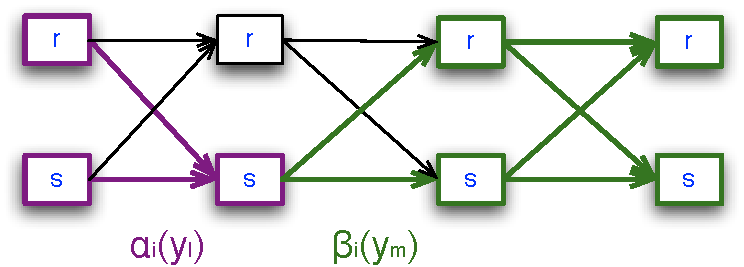
\includegraphics[scale=.5]{figs/sequences/statePost}
%& 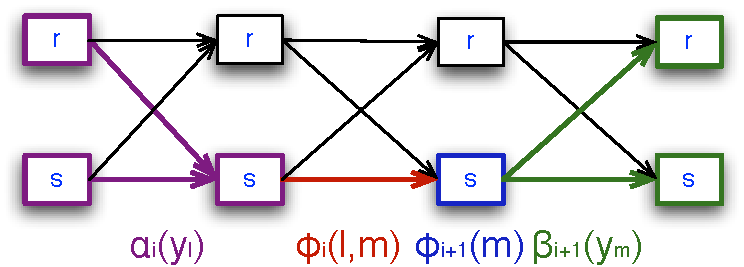
\includegraphics[scale=.5]{figs/sequences/transPost}\\
%\end{tabular}
%\caption[Posterior Illustration.]{\label{fig:posteriors} A graphical representation of the components in the state and transition posteriors.}
%
%\end{center}
%\end{figure}

Using the state posteriors, we are ready to perform posterior
decoding. 
The strategy is to compute the state posteriors 
for each position $i \in \{1,\ldots,N\}$
and each state $c_k \in \statevocab$, and 
then pick the arg-max at each position:
\begin{equation}
{\widehat y_i} := \argmax_{y_i \in \statevocab} P(Y_i=y_i| X=x).
\end{equation}

%Algorithm \ref{alg:pd} shows the posterior decoding algorithm.

%\begin{algorithm}[t]
%   \caption{Posterior Decoding algorithm \label{alg:pd}}
%\begin{algorithmic}[1]
%   \STATE {\bfseries input:} The forward and backward probabilities
%       $\alpha$ and $\beta$.
%   \STATE  \emph{Compute Likelihood}: Compute the likelihood of the
%   sentence
%   \STATE $L = 0$
%   \FOR{$\hv_l \in \hvocab$ }
%   \STATE $\marginal = \marginal + \alpha_N(\hv_l)$
%   \ENDFOR 
%   \STATE $\hat \hseq = []$
%    \FOR{$i=1$ {\bfseries to} $N$}
%    \STATE $max = 0$
%     \FOR{$\hv_l \in \hvocab$ }
%     \STATE $\gamma_i(\hv_l)  =  \frac{\alpha_i(\hv_l)
%       \beta_i(\hv_l)}{\marginal}$
%     \IF {$\gamma_i(\hv_l) > max$}
%     \STATE $max = \gamma_i(\hv_l)$
%     \STATE $\hat  y_i = \hv_l$
%     \ENDIF
%     \ENDFOR 
%     \ENDFOR 
%   \STATE \textbf{output:} the posterior path $\hat \hseq$
%\end{algorithmic}
%\end{algorithm}


\newpage
\begin{exercise}
%Given the node and edge posterior formulas \ref{eq::nodePosterior},\ref{eq::edgePosterior} and the
%  forward and backward formulas \ref{eq::forward},\ref{eq::backward}, convince yourself that formulas
%  \ref{eq::nodePosterior2},\ref{eq::edgePosterior2} are correct. 

Compute the node posteriors for the first training sequence (use the provided \emph{compute\_posteriors} function), and look at
the output. Note that the state posteriors are a proper
probability distribution (the lines of the result sum to 1).

\begin{python}
initial_scores, transition_scores, final_scores, emission_scores = hmm.compute_scores(simple.train.seq_list[0])
state_posteriors, _, _ = hmm.compute_posteriors(initial_scores,
                                                transition_scores,
                                                final_scores,
                                                emission_scores)
print state_posteriors

[[ 0.95738152  0.04261848]
 [ 0.75281282  0.24718718]
 [ 0.26184794  0.73815206]
 [ 0.          1.        ]]
\end{python}
\end{exercise}

\begin{exercise}
Run the posterior decode on the first test sequence, and evaluate it.
\begin{python}
y_pred = hmm.posterior_decode(simple.test.seq_list[0])
print "Prediction test 0:", y_pred

walk/rainy walk/rainy shop/sunny clean/sunny

print "Truth test 0:", simple.test.seq_list[0]

walk/rainy walk/sunny shop/sunny clean/sunny 
\end{python}

Do the same for the second test sequence:
\begin{python}
y_pred = hmm.posterior_decode(simple.test.seq_list[1])
print "Prediction test 1:", y_pred

clean/rainy walk/rainy tennis/rainy walk/rainy 

print "Truth test 1:", simple.test.seq_list[1]

clean/sunny walk/sunny tennis/sunny walk/sunny 
\end{python}

What is wrong? Note the observations for the second test sequence: the
observation {\tt tennis} was never seen at training time, so the probability for
it will be zero (no matter what state). This will make all possible state
sequences have zero probability.
As seen in the previous lecture, this is a problem with generative
models, which can be corrected using smoothing (among other
options).

Change the \emph{train\_supervised} method to add smoothing:
\begin{python}
def train_supervised(self,sequence_list, smoothing):
\end{python}

Try, for example, adding 0.1 to all the counts, and repeating this exercise with that smoothing. What do you observe?
\begin{python}
hmm.train_supervised(simple.train, smoothing=0.1)
y_pred = hmm.posterior_decode(simple.test.seq_list[0])
print "Prediction test 0 with smoothing:", y_pred

walk/rainy walk/rainy shop/sunny clean/sunny 

print "Truth test 0:", simple.test.seq_list[0]

walk/rainy walk/sunny shop/sunny clean/sunny

y_pred = hmm.posterior_decode(simple.test.seq_list[1])
print "Prediction test 1 with smoothing:", y_pred

clean/sunny walk/sunny tennis/sunny walk/sunny 

print "Truth test 1:", simple.test.seq_list[1]

clean/sunny walk/sunny tennis/sunny walk/sunny 
\end{python}
\end{exercise}

%Note that if you use smoothing when training, the sanity checks mentioned at the start of this chapter are no longer true. For example, the sum of all the transition counts is no longer equal to the number of tokens -- it is larger.

%\begin{exercise}
%Change the function you just created \emph{ def
%  sanity\_check\_counts(self,seq\_list):} to account for smoothing. Make
%sure it works properly.
%
%\begin{python}
%In []: run sequences/hmm.py
%In []: hmm = HMM(simple)
%In []: hmm.collect_counts_from_corpus(simple.train,smoothing=0.1)
%In []: hmm.sanity_check_counts(simple.train,smoothing=0.1)
%Init Counts match
%Final Counts match
%Transition Counts match
%Observations Counts match
%\end{python}
%\end{exercise}


\subsection{Viterbi Decoding}\label{viterbi}


\textbf{Viterbi decoding} consists in
picking the best global hidden state sequence 
$\widehat{y}$
as follows: 
\begin{equation}
\widehat{y} = \argmax_{y \in \statevocab^N} P(Y=y|X=x) = \argmax_{y \in \statevocab^N} P(X=x,Y=y).
\end{equation}

The Viterbi algorithm 
is very similar to the forward procedure of the FB algorithm,
making use of the same trellis structure to efficiently represent the exponential number of sequences without prohibitive computation costs. In fact, the only
difference from the forward-backward algorithm is in the recursion
\ref{forwardRecursion} where instead of \emph{summing} over all possible 
hidden states, we take their \emph{maximum}.

\begin{equation}
\label{eq::viterbi}
\mathbf{Viterbi }\;\;\;\;  \mathrm{viterbi}(i, y_i) = \max_{y_1...y_{i-1}} P(Y_1=y_1,\ldots Y_i = y_i , X_1=x_1,\ldots, X_i=x_i)
\end{equation}
The Viterbi trellis represents the path with maximum probability in
position
$i$ when we are in state $Y_i=y_i$ and that we have observed $x_1,\ldots,x_i$
up to that position. The Viterbi algorithm is defined by the
following recurrence: 
\begin{eqnarray}
\mathrm{viterbi}(1, c_k) &=& P_{\mathrm{init}}(c_k|\text{\tt start}) \times 
P_{\mathrm{emiss}}(x_1 | c_k)
 \\
 \mathrm{viterbi}(i, c_k) &=& \left( \displaystyle \max_{c_l \in \statevocab} P_{\mathrm{trans}}(c_k | c_l) \times \mathrm{viterbi}(i-1, c_l) \right) \times P_{\mathrm{emiss}}(x_i | c_k)  \label{viterbiRecursion}
 \\
 \mathrm{backtrack}(i, c_k) &=& \left( \displaystyle \argmax_{c_l \in \statevocab} P_{\mathrm{trans}}(c_k | c_l) \times \mathrm{viterbi}(i-1, c_l) \right) 
 \\
  \mathrm{viterbi}(N+1, \text{\tt stop}) &=& \max_{c_l \in \statevocab} P_{\mathrm{final}}(\text{\tt stop} | c_l) \times \mathrm{viterbi}(N, c_l)
 \\
  \mathrm{backtrack}(N+1, \text{\tt stop}) &=& \argmax_{c_l \in \statevocab} P_{\mathrm{final}}(\text{\tt stop} | c_l) \times \mathrm{viterbi}(N, c_l).
\end{eqnarray}


%\begin{eqnarray}
%\delta_1(\hv_l) &=& \phi_1(l) \\
%\delta_i(\hv_l) &=& \left[ \max_{y_1 ... y_i} \phi_{i-1,i}(m,l)
%  \delta_{i-1}(\hv_m) \right] \phi_i(l) \label{viterbiRecursion} \\
%\psi_{i}(\hv_l) &=& \left[ \argmax_{y_1 ... y_i} \phi_{i-1,i}(m,l)
%  \delta_{i-1}(\hv_m) \right]
%%\phi_{(i-1)}(m,l)  \delta_{i-1}(\hv_m) \right] \phi_i(l) \label{viterbiBackpointers}
%\end{eqnarray}

Algorithm \ref{alg:viterbi} shows the pseudo code for the Viterbi algorithm.
Note the similarity with the forward algorithm.
The only differences are:
\begin{itemize}
\item Maximizing instead of summing;
\item Keeping the argmax's to backtrack.
\end{itemize}

%\begin{algorithm}[t]
%   \caption{Viterbi algorithm \label{alg:viterbi}}
%\begin{algorithmic}[1]
%   \STATE {\bfseries input:} sentence $\sent$, parameters $\theta$
%        \STATE  \emph{Forward pass}: compute the maximum paths for
%        every end state
%        \STATE \emph{Initialization}
%        \FOR{$\hv_l \in \hvocab$ }
%        \STATE $\delta_1(\hv_l) = \phi_1(\hv_l)$
%        \ENDFOR 
%        \FOR{$i=2$ {\bfseries to} $N$}
%         \FOR{$\hv_l \in \hvocab$ }
%                 \STATE $\delta_i(\hv_l) = \left[ \displaystyle
%                   \max_{m  \in \hvocab} \phi_{i-1,i}(m,l)
%                   \delta_{i-1}(\hv_m) \right] \phi_i(l)$
%                 \STATE $\psi_{i}(\hv_l) = m$
%         \ENDFOR 
%        \ENDFOR 
%       %\STATE \emph{Terminate}:
%       \STATE 
%  $\max_{y \in \statevocab^N} P(X=x,Y=y) := \max_{c_l \in \statevocab} P_{\mathrm{final}}(\text{\tt stop} | c_l) \times \mathrm{viterbi}(N, c_l)$
%  	   \STATE 
%       \STATE \emph{Backward pass}: Build the most likely path
%	  \STATE $\widehat{y}_i = \argmax_{c_l \in \statevocab} P_{\mathrm{final}}(\text{\tt stop} | c_l) \times \mathrm{viterbi}(N, c_l)$ 
%	   \FOR{$i=N-1$ {\bfseries to} 1}
%        \STATE $\widehat{y_i} = \mathrm{backtrack}(i+1, \widehat{y}_{i+1})$
%        \ENDFOR 
%       \STATE \textbf{output:} the viterbi path $\widehat{y}$
%\end{algorithmic}
%\end{algorithm}

\begin{algorithm}[t]
   \caption{Viterbi algorithm \label{alg:viterbi}}
\begin{algorithmic}[1]
   \STATE {\bfseries input:} sequence $x_1,\ldots,x_N$, scores $P_{\mathrm{init}}, P_{\mathrm{trans}}, P_{\mathrm{final}}, P_{\mathrm{emiss}}$
        \STATE  \emph{Forward pass}: Compute the best paths for every end state
        \STATE \emph{Initialization}
        \FOR{$c_k \in \statevocab$ }
        \STATE $\mathrm{viterbi}(1,c_k) = P_{\mathrm{init}}(c_k|\text{\tt start}) \times 
P_{\mathrm{emiss}}(x_1 | c_k)$
        \ENDFOR 
        \FOR{$i=2$ {\bfseries to} $N$}
         \FOR{$c_k \in \statevocab$ }
          \STATE $\mathrm{viterbi}(i, c_k) = \left( \displaystyle \max_{c_l \in \statevocab} P_{\mathrm{trans}}(c_k | c_l) \times \mathrm{viterbi}(i-1, c_l) \right) \times P_{\mathrm{emiss}}(x_i | c_k)$
          \STATE $\mathrm{backtrack}(i, c_k) = \left( \displaystyle \argmax_{c_l \in \statevocab} P_{\mathrm{trans}}(c_k | c_l) \times \mathrm{viterbi}(i-1, c_l) \right)$
         \ENDFOR 
        \ENDFOR 
       \STATE 
  $\max_{y \in \statevocab^N} P(X=x,Y=y) := \max_{c_l \in \statevocab} P_{\mathrm{final}}(\text{\tt stop} | c_l) \times \mathrm{viterbi}(N, c_l)$        
        \STATE
       \STATE \emph{Backward pass}: backtrack to obtain the most likely path 
	  \STATE $\widehat{y}_N = \argmax_{c_l \in \statevocab} P_{\mathrm{final}}(\text{\tt stop} | c_l) \times \mathrm{viterbi}(N, c_l)$ 
	   \FOR{$i=N-1$ {\bfseries to} 1}
        \STATE $\widehat{y_i} = \mathrm{backtrack}(i+1, \widehat{y}_{i+1})$
        \ENDFOR 
       \STATE \textbf{output:} the viterbi path $\widehat{y}$.
\end{algorithmic}
\end{algorithm}

\section{Assignment}

With the previous theoretical background, you have the necessary tools to solve today's assignment.

\begin{exercise}
Implement a method 
for performing Viterbi decoding in 
file {\tt sequence\_classification\_decoder.py}.
\begin{python}
        def run_viterbi(self, initial_scores, transition_scores, final_scores, emission_scores):
\end{python}
Hint: look at the implementation of {\tt run\_forward}. Also check the help for the numpy methods max and argmax.

This method will be called 
by 
\begin{python}
def viterbi_decode(self, sequence)
\end{python}
in the module {\tt sequence\_classifier.py}.
%
%posterior decoding (the function \emph{posterior\_decode}) for reference.

Test your method on both test sequences and compare the results with
the ones given.
\begin{python}
hmm.train_supervised(simple.train, smoothing=0.1)
y_pred, score = hmm.viterbi_decode(simple.test.seq_list[0])
print "Viterbi decoding Prediction test 0 with smoothing:", y_pred, score

walk/rainy walk/rainy shop/sunny clean/sunny  -6.02050124698

print "Truth test 0:", simple.test.seq_list[0]

walk/rainy walk/sunny shop/sunny clean/sunny 

y_pred, score = hmm.viterbi_decode(simple.test.seq_list[1])
print "Viterbi decoding Prediction test 1 with smoothing:", y_pred, score

clean/sunny walk/sunny tennis/sunny walk/sunny  -11.713974074

print "Truth test 1:", simple.test.seq_list[1]

clean/sunny walk/sunny tennis/sunny walk/sunny 
\end{python}

Note: since we didn't run the \emph{train\_supervised} method again, we are still using the result of the training using smoothing. Therefore, you should compare these results to the ones of posterior decoding with smoothing.

\end{exercise}




%%% Local Variables: 
%%% mode: latex
%%% TeX-master: "../../guide"
%%% End: 


\section{\label{pos-tagging} Part-of-Speech Tagging (POS)}
Part-of-Speech (PoS) tagging is one of the most important NLP tasks. The
task is to assign each word a grammatical category, or Part-of-Speech, \emph{i.e.} noun,
verb, adjective,... Recalling the defined notation, $\vocab$ is a 
vocabulary of word types, and 
$\statevocab$ is the set of Part-of-Speech tags.

In English, using the Penn Treebank (PTB) corpus \citep{pennTreeBank}, the current
state of the art for part of speech tagging is around 97\% for a
variety of methods.

In the rest of this class we will use a subset of the PTB corpus, but
instead of using the original 45 tags we will use a reduced tag set of
12 tags, to make the algorithms faster for the
class. In this task, $x$ is a sentence (\emph{i.e.}, a sequence of word tokens) and $y$
is the sequence of possible PoS tags.

The first step is to load the corpus. We will start by loading
1000 sentences for training and 1000 sentences both for development and
testing. Then we train the HMM model by maximum likelihood estimation.
\begin{python}
import lxmls.readers.pos_corpus as pcc
corpus = pcc.PostagCorpus()
train_seq = corpus.read_sequence_list_conll("data/train-02-21.conll",max_sent_len=15,max_nr_sent=1000)
test_seq = corpus.read_sequence_list_conll("data/test-23.conll",max_sent_len=15,max_nr_sent=1000)
dev_seq = corpus.read_sequence_list_conll("data/dev-22.conll",max_sent_len=15,max_nr_sent=1000)
hmm = hmmc.HMM(corpus.word_dict, corpus.tag_dict)
hmm.train_supervised(train_seq)
hmm.print_transition_matrix()
\end{python}


Look at the transition probabilities of the trained model
%\begin{python}
%In []: import matplotlib.pyplot as plt
%In []: hmm.transition_probs
%\end{python}
 (see
Figure \ref{fig:transProbs}), and see if they match your intuition
about the English language (e.g. adjectives tend to come before nouns).

\begin{figure}[h!]
\centering
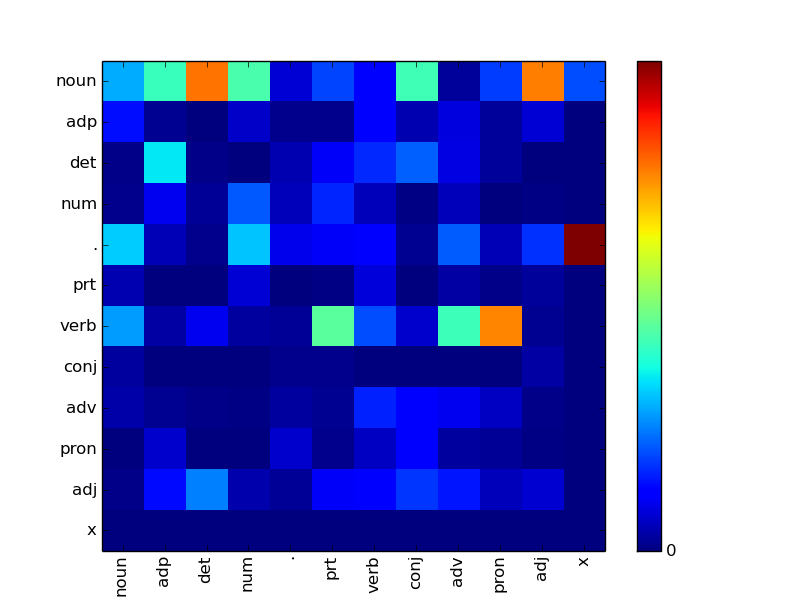
\includegraphics[scale=.5]{figs/sequences/transition_probs}
\caption{\label{fig:transProbs} Transition probabilities of the
trained model. Each column is the previous state and row is the current
state. Note the high probability of having Noun after Determinant or Adjective, or of having Verb after Nouns or Pronouns, as expected.}
\end{figure}

\begin{exercise}
Test the model using both posterior decoding and Viterbi decoding on
both the train and test set, using the methods in class HMM:
\begin{python}
viterbi_pred_train = hmm.viterbi_decode_corpus(train_seq)
posterior_pred_train = hmm.posterior_decode_corpus(train_seq)
eval_viterbi_train =   hmm.evaluate_corpus(train_seq, viterbi_pred_train)
eval_posterior_train =  hmm.evaluate_corpus(train_seq, posterior_pred_train)
print "Train Set Accuracy: Posterior Decode \%.3f, Viterbi Decode: \%.3f"\%(eval_posterior_train,eval_viterbi_train)

Train Set Accuracy: Posterior Decode 0.985, Viterbi Decode: 0.985

viterbi_pred_test = hmm.viterbi_decode_corpus(test_seq)
posterior_pred_test = hmm.posterior_decode_corpus(test_seq)
eval_viterbi_test =   hmm.evaluate_corpus(test_seq,viterbi_pred_test)
eval_posterior_test = hmm.evaluate_corpus(test_seq,posterior_pred_test)
print "Test Set Accuracy: Posterior Decode \%.3f, Viterbi Decode: \%.3f"\%(eval_posterior_test,eval_viterbi_test)

Test Set Accuracy: Posterior Decode 0.350, Viterbi Decode: 0.509
\end{python}
What do you observe? Remake the previous exercise but now train the HMM
using smoothing. Try different values (0,0.1,0.01,1) and report the results on the
train and development set. (Use function
\emph{pick\_best\_smoothing}).


\begin{python}
best_smoothing = hmm.pick_best_smoothing(train_seq, dev_seq, [10,1,0.1,0])

Smoothing 10.000000 --  Train Set Accuracy: Posterior Decode 0.731, Viterbi Decode: 0.691
Smoothing 10.000000 -- Test Set Accuracy: Posterior Decode 0.712, Viterbi Decode: 0.675
Smoothing 1.000000 --  Train Set Accuracy: Posterior Decode 0.887, Viterbi Decode: 0.865
Smoothing 1.000000 -- Test Set Accuracy: Posterior Decode 0.818, Viterbi Decode: 0.792
Smoothing 0.100000 --  Train Set Accuracy: Posterior Decode 0.968, Viterbi Decode: 0.965
Smoothing 0.100000 -- Test Set Accuracy: Posterior Decode 0.851, Viterbi Decode: 0.842
Smoothing 0.000000 --  Train Set Accuracy: Posterior Decode 0.985, Viterbi Decode: 0.985
Smoothing 0.000000 -- Test Set Accuracy: Posterior Decode 0.370, Viterbi Decode: 0.526

hmm.train_supervised(train_seq, smoothing=best_smoothing)
viterbi_pred_test = hmm.viterbi_decode_corpus(test_seq)
posterior_pred_test = hmm.posterior_decode_corpus(test_seq)
eval_viterbi_test =   hmm.evaluate_corpus(test_seq, viterbi_pred_test)
eval_posterior_test = hmm.evaluate_corpus(test_seq, posterior_pred_test)
print "Best Smoothing \%f --  Test Set Accuracy: Posterior Decode \%.3f, Viterbi Decode: \%.3f"%(best_smoothing,eval_posterior_test,eval_viterbi_test)

Best Smoothing 0.100000 --  Test Set Accuracy: Posterior Decode 0.837, Viterbi Decode: 0.827
\end{python}


Perform some error analysis to understand were the errors are coming
from. You can start by visualizing the confusion matrix (true tags vs
predicted tags). You should get something like what is shown in Figure~\ref{fig:cmuns}.

\begin{python}
import lxmls.sequences.confusion_matrix as cm
import matplotlib.pyplot as plt
confusion_matrix = cm.build_confusion_matrix(test_seq.seq_list, viterbi_pred_test, len(corpus.tag_dict), hmm.get_num_states())
cm.plot_confusion_bar_graph(confusion_matrix, corpus.tag_dict, xrange(hmm.get_num_states()), 'Confusion matrix')
plt.show()
\end{python}

\begin{figure}[h!]
\centering
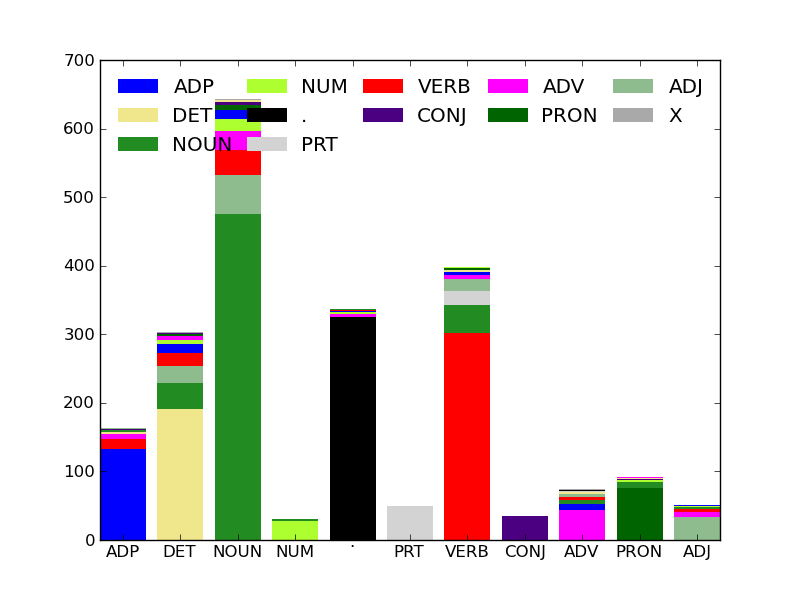
\includegraphics[scale=.4]{figs/sequences/cm_sup.png}
\caption{\label{fig:cmuns} Confusion Matrix for the previous
  example. Predicted tags are columns and the true tags corresponds to
  the constituents of each column.}
\end{figure}

\end{exercise}


%\begin{exercise}
%Implement a function that produces the accuracy for rare words vs
%common words. Use you own definition of rare word.
%
%Can you come up with other error analysis methods? Which?
%
%\end{exercise}

%\begin{exercise}
%So far we have only worked with a limited dataset of 1000 words. Try increasing the number of sentences to 10000. What do you observe?
%\end{exercise}


%\section{Unsupervised Learning of HMMs}
%
%\afm{explain here the EM algorithm}
%
%\begin{python}
%
%Initial accuracy: 0.303638
%Iter: 1 Log Likelihood: -101824.763927
%Iter: 1 Accuracy: 0.305441
%Iter: 2 Log Likelihood: -78057.108346
%Iter: 2 Accuracy: 0.321976
%Iter: 3 Log Likelihood: -77813.725501
%Iter: 3 Accuracy: 0.357451
%Iter: 4 Log Likelihood: -77192.947674
%Iter: 4 Accuracy: 0.385109
%Iter: 5 Log Likelihood: -76191.800849
%Iter: 5 Accuracy: 0.392123
%Iter: 6 Log Likelihood: -75242.572729
%Iter: 6 Accuracy: 0.391121
%Iter: 7 Log Likelihood: -74392.892496
%Iter: 7 Accuracy: 0.404249
%Iter: 8 Log Likelihood: -73357.542833
%Iter: 8 Accuracy: 0.399940
%Iter: 9 Log Likelihood: -72135.182778
%Iter: 9 Accuracy: 0.399238
%Iter: 10 Log Likelihood: -70924.246230
%Iter: 10 Accuracy: 0.395430
%Iter: 11 Log Likelihood: -69906.561800
%Iter: 11 Accuracy: 0.394328
%Iter: 12 Log Likelihood: -69140.228623
%Iter: 12 Accuracy: 0.390821
%Iter: 13 Log Likelihood: -68541.416423
%Iter: 13 Accuracy: 0.391522
%Iter: 14 Log Likelihood: -68053.456865
%Iter: 14 Accuracy: 0.389117
%Iter: 15 Log Likelihood: -67667.318961
%Iter: 15 Accuracy: 0.386411
%Iter: 16 Log Likelihood: -67337.685686
%Iter: 16 Accuracy: 0.385409
%Iter: 17 Log Likelihood: -67054.571821
%Iter: 17 Accuracy: 0.385409
%Iter: 18 Log Likelihood: -66769.973881
%Iter: 18 Accuracy: 0.385409
%Iter: 19 Log Likelihood: -66442.608458
%Iter: 19 Accuracy: 0.385409
%
%\end{python}



%\section{\label{hmm_special_state} HMM Initial and Final State}
%\input{pages/sequences/init_final_hmm.tex}

%\section{\label{hmm} Second order HMM}
%
\subsection{State Expansion}

The ideia here is to expand the states and use the same inference
procedures as those of the HMM.



\subsection{Modelling second order}

Here we use the original states and we derive new inference procedures....

\begin{eqnarray*}
\alpha_{t=2}(1) &=& P(y_{t=2} = 1,x_0,x_1,x_2) = \sum_{b \in \hvocab}
\sum_{a\in \hvocab} P(y_{t=2} = 1,x_0,x_1,x_2, y_{t=0}=a,y_{t=1}=b)\\
\alpha_{t=2}(1) &=& \sum_{b \in \hvocab}
\sum_{a\in \hvocab}
p(x_2 |  y_{t=2}) p(y_{t=2} | y_{t=1} =b ,y_{t=0}=a)  p(x_1 |  y_{t=1}
=b) p(y_{t=1} =b| y_{t=0}=a)\\
&*&  p(x_0 |  y_{t=0}=a) p(y_{t=0}=a) \\
\alpha_{t=2}(1) &=& \sum_{b \in \hvocab}
\sum_{a\in \hvocab}
p(x_2 |  y_{t=2}) p(y_{t=2} | y_{t=1} = b,y_{t=0} = a)  p(x_1 |
y_{t=1} = b) p(y_{t=1} = b| y_{t=0} = a)  \mathbf{p(x_0 ,  y_{t=0} = a) }\\
\alpha_{t=2}(1) &=& \sum_{b \in \hvocab}
\sum_{a\in \hvocab}
p(x_2 |  y_{t=2}) p(y_{t=2} | y_{t=1} = b,y_{t=0} = a)  p(x_1 |
y_{t=1} = b) p(y_{t=1} = b| y_{t=0} = a)  \alpha_{t=0}(a) \\
\alpha_{t=2}(1) &=& \sum_{b \in \hvocab}
\sum_{a\in \hvocab}
p(x_2 |  y_{t=2}) p(y_{t=2} | y_{t=1} = b,y_{t=0} = a)  p(x_1 ,
y_{t=1} = b | y_{t=0} = a)  \alpha_{t=0}(a) \\
\alpha_{t=2}(1) &=& \sum_{b \in \hvocab}
\sum_{a\in \hvocab}
p(x_2 |  y_{t=2}) p(y_{t=2} | y_{t=1} = b,y_{t=0} = a)  \mathbf{p(x_1 ,
y_{t=1} = b ,x_0 ,  y_{t=0} = a) }
\end{eqnarray*}

%%% Local Variables: 
%%% mode: latex
%%% TeX-master: "../../guide"
%%% End: 


%%% Local Variables: 
%%% mode: latex
%%% TeX-master: "../../guide.tex"
%%% End: 


\chapter{\label{day:seq_disc}Learning Structured Predictors}
In this class, we will continue to focus on sequence classification,
but instead of following a \emph{generative} approach (like in the previous
chapter) we move towards \emph{discriminative} approaches. Recall that the difference between these approaches is that generative approaches attempt to model the probability distribution of the data, $P(X,Y)$, whereas discriminative ones only model the conditional probability of the sequence, given the observed data, $P(Y|X)$.



\section*{Today's Assignment}

The assignment of today's class is to implement the structured version of the perceptron algorithm.

\section{Classification vs Sequential Classification}


Table \ref{disc_seq_summary} shows how the models for classification 
have counterparts in \emph{sequential} classification. In fact, in
the last chapter we discussed the Hidden Markov model, which can be seen as a
generalization of the Na\"{i}ve Bayes model for sequences. 
In this chapter, we will see a generalization of the
Perceptron algorithm for sequence problems (yielding the Structured
Perceptron, \citealt{collins2002discriminative}) and a generalization of
Maximum Entropy model for sequences (yielding Conditional Random Fields, \citealt{lafferty2001conditional}). 
Note that both these generalizations are  not specific for sequences
and can be applied to a wide range of models (we will see in tomorrow's
lecture how these methods can be applied to parsing).
Although we will not cover all the methods described in
Chapter \ref{day:classification}, bear in mind that all of those have a structured counterpart. 
It should be intuitive after this lecture how those methods could be
extended to structured problems, given the perceptron example.
%Before we explain the particular methods, the next section will talk a bit about feature representation for sequences. 

\begin{table}[h!]
\centering
\begin{tabular}{|l|l|}
\hline
\multicolumn{1}{|c|}{\textbf{Classification}} & \multicolumn{1}{|c|}{\textbf{Sequences}} \\
\hline
\multicolumn{2}{|c|}{\emph{Generative}}\\
\hline
Na\"{i}ve Bayes~(Sec.~\ref{s::naiveBayes}) & Hidden Markov Models~(Sec.~\ref{hmm}) \\
\hline
\multicolumn{2}{|c|}{\emph{Discriminative}}\\
\hline
Perceptron~(Sec.~\ref{s:perceptron}) & Structured Perceptron~(Sec.~\ref{s:spercetron})\\
\hline
Maximum Entropy~(Sec.~\ref{s:me}) & Conditional Random Fields~(Sec.~\ref{s:crf})\\
\hline
\end{tabular}
\caption{\label{disc_seq_summary}Summary of the methods used for classification and sequential classification covered in this guide.}
\end{table}


Throughout this chapter, we will be searching for the solution of 
\begin{equation}
\argmax_{y \in \statevocab^N} P(Y=y | X=x) = \argmax_{y \in \statevocab^N} \W \cdot  \F(x,y). \label{eq::struc_pred} 
\end{equation}
where $\W$ is a weight vector, and $\F(x,y)$ is a feature vector. We will see that this sort of linear models are more flexible than HMMs, in the sense that they may incorporate 
more general features while being able to reuse the same decoders (based on the Viterbi and forward-backward algorithms). In fact, \emph{the exercises in this lab will not touch the decoders that 
have been developed in the previous lab}. 
Only the training algorithms and the function that 
compute the scores will change.

As in the previous section, $y = y_1\ldots y_N$ is a sequence so the maximization
is over an exponential number of objects, making it intractable for brute force methods. Again
we will make an assumption analogous to the ``first order Markov independence property,'' so that the
features may decompose as a sum over nodes and edges in a trellis. 
This is done by assuming that expression~\ref{eq::struc_pred} can be written as:
\begin{equation}
\argmax_{y \in \statevocab^N} 
\sum_{i=1}^N \underbrace{\W \cdot \F_{\mathrm{emiss}}(i,x,y_i)}_{\mathrm{score}_{\mathrm{emiss}}}  + 
\underbrace{\W \cdot \F_{\mathrm{init}}(x,y_1)}_{\mathrm{score}_{\mathrm{init}}}  + 
\sum_{i=1}^{N-1} \underbrace{\W \cdot \F_{\mathrm{trans}}(i,x,y_i,y_{i+1})}_{\mathrm{score}_{\mathrm{trans}}}+ 
\underbrace{\W \cdot \F_{\mathrm{final}}(x,y_N)}_{\mathrm{score}_{\mathrm{final}}}
\label{eq::struc_pred_decompose}
\end{equation}
In other words, the scores ${\mathrm{score}_{\mathrm{emiss}}}$, 
${\mathrm{score}_{\mathrm{init}}}$, ${\mathrm{score}_{\mathrm{trans}}}$
and ${\mathrm{score}_{\mathrm{final}}}$ are now computed as inner products 
between weight vectors and feature vectors rather than log-probabilities.
The feature vectors depend locally on the output variable 
(\emph{i.e.}, they only look at a single $y_i$ or a pair $y_i,y_{i+1}$);
however they may depend globally on the observed input $x=x_{1},\ldots,x_{N}$.


\section{\label{seq::features} Features}

In this section we will define two simple feature sets.\footnote{Although not required, all the features we will use are binary features, indicating whether a given condition 
is satisfied or not.} The first feature set
will only use identity features, and will mimic the features used by
the HMM model from the previous section. This will allow us to directly
compare the performance of a generative vs a discriminative
approach. %\begin{example}
%Simple ID Feature set containing the same features as an HMM model.
%\begin{python}
%0 Ms./NOUN NF: id:Ms.::NOUN init_tag:NOUN 
%1 Haag/NOUN NF: id:Haag::NOUN EF: prev_tag:NOUN::NOUN 
%2 plays/VERB NF: id:plays::VERB EF: prev_tag:NOUN::VERB 
%3 Elianti/NOUN NF: id:Elianti::NOUN EF: prev_tag:VERB::NOUN 
%4 ./. NF: id:.::. EF: last_prev_tag:NOUN::. 
%\end{python}
%\end{example}
Table~\ref{id-features} depicts the features that are implicit in the HMM, which was the subject of 
the previous chapter. These features are indicators of initial, transition, final, and emission events.

\begin{table}[h!]
\begin{center}
\begin{tabular}{|l|l|}
\hline
Condition & Name\\
\hline
$y_i = c_k \text{  } \& \text{  } i =0 $& Initial Features \\
\hline
$y_i = c_k \text{  } \& \text{  } y_{i-1} = c_l$& Transition Features \\
\hline
$y_i = c_k \text{  } \& \text{  } i = N$& Final Features \\
\hline
$x_i = w_j \text{  } \& \text{  } y_i = c_k$ & Emission Features \\
\hline
\end{tabular}
\caption{\label{id-features} {\tt IDFeatures} feature set. This set
  replicates the features used by the HMM model.}
\end{center}
\end{table}
 
 
Note that the fact that we were using a generative model has forced us (in some sense) to 
make strong independence assumptions. 
However, since we now move to a discriminative approach, where we model $P(Y|X)$ rather than $P(X,Y)$, we are not tied anymore to 
some of these assumptions. In particular: 
\begin{itemize}
\item We may use ``overlapping'' features, \emph{e.g.}, features that fire simultaneously for many instances. 
For example, we can use a feature for a word, such as a feature which fires for the word "brilliantly", and another for prefixes and suffixes of that word, such as one which fires if the last two letters of the word are "ly".
This would lead to an awkward model if we wanted to insist on a generative approach. 
\item We may use features that depend arbitrarily on the \emph{entire input sequence} $x$. On the other hand, 
we still need to resort to ``local'' features with respect to the \emph{outputs} (\emph{e.g.} looking only at consecutive state pairs), 
otherwise decoding algorithms will become more expensive.  
\end{itemize}


This leads us to the second feature set, composed of features that are traditionally used in POS tagging with discriminative models. See Table~\ref{ex-features} for some examples.
Of course, we could have much more complex features, looking arbitrarily to 
the input sequence. We are not going to have them in this
exercise only for performance reasons (to have less features and smaller caches). State-of-the-art sequence classifiers can easily reach over one million features!

\begin{table}[h!]
\begin{center}
\begin{tabular}{|l|l|}
\hline
Condition & Name\\
\hline
$y_i = c_k \text{  } \& \text{  } i =0 $& Initial Features \\
\hline
$y_i = c_k \text{  } \& \text{  } y_{i-1} = c_l$& Transition Features \\
\hline
$y_i = c_k \text{  } \& \text{  } i = N$& Final Features \\
\hline
$x_i = w_j \text{  } \& \text{  } y_i = c_k$& Basic Emission Features \\
$x_i = w_j \text{  } \& \text{ $w_j$ is uppercased} \text{  } \& \text{  } y_i = c_k$& Uppercase Features
\\
$x_i = w_j \text{  } \& \text{ $w_j$ contains digit} \text{  } \& \text{  } y_i = c_k$& Digit Features
\\
$x_i = w_j \text{  } \& \text{ $w_j$ contains hyphen} \text{  } \& \text{  } y_i = c_k$& Hyphen Features
\\
$x_i = w_j \text{  } \& \text{  } w_j[0..i] \forall i \in [1,2,3]
\text{  } \& \text{  } y_i = c_k$& Prefix Features \\
$x_i = w_j \text{  } \& \text{  } w_j[|w_j|-i..|w_j|] \forall i \in [1,2,3] \text{  } \& \text{  } y_i = c_k$& Suffix Features \\
\hline
\end{tabular}
\caption{\label{ex-features} {\tt Extended} feature set. Some features in this set could not be included in the HMM model. The features included in the bottom row are all considered emission features 
for the purpose of our implementation, since they all depend on $i$, $x$ and $y_i$.}
\end{center}
\end{table}



%\begin{example}
%
%\begin{python}
%0 Ms./NOUN NF: id:Ms.::NOUN uppercased::NOUN suffix:.::NOUN suffix:s.::NOUN prefix:M::NOUN prefix:Ms::NOUN init_tag:NOUN 
%1 Haag/NOUN NF: id:Haag::NOUN uppercased::NOUN suffix:g::NOUN suffix:ag::NOUN suffix:aag::NOUN prefix:H::NOUN prefix:Ha::NOUN prefix:Haa::NOUN rare::NOUN EF: prev_tag:NOUN::NOUN 
%2 plays/VERB NF: id:plays::VERB EF: prev_tag:NOUN::VERB 
%3 Elianti/NOUN NF: id:Elianti::NOUN uppercased::NOUN suffix:i::NOUN suffix:ti::NOUN suffix:nti::NOUN prefix:E::NOUN prefix:El::NOUN prefix:Eli::NOUN rare::NOUN EF: prev_tag:VERB::NOUN 
%4 ./. NF: id:.::. EF: last_prev_tag:NOUN::. 
%\end{python}
%\end{example}



Our features subdivide into two groups: 
$\F_{\mathrm{emiss}}$, $\F_{\mathrm{init}}$, 
and $\F_{\mathrm{final}}$ are all instances of 
\emph{node features}, 
depending only on a single position in the
state sequence (a node in the trellis); 
$\F_{\mathrm{trans}}$ 
are \emph{edge features},
depending on two consecutive positions in the state 
sequence (an edge in the trellis).
Similarly as in the previous chapter, we have the following scores (also called 
\emph{log-potentials} in the literature on CRFs and graphical models):
\begin{itemize}
\item \emph{Initial scores.}
These are scores for the initial state. 
They are given by 
\begin{equation}
{\mathrm{score}}_{\mathrm{init}}(x,y_1) = \W \cdot \F_{\mathrm{init}}(x,y_1).
\end{equation} 
\item \emph{Transition scores.}
These are scores for two consecutive states at a particular position. 
They are given by 
\begin{equation}
{\mathrm{score}}_{\mathrm{trans}}(i,x,y_i,y_{i+1}) = \W \cdot \F_{\mathrm{trans}}(i,x,y_{i},y_{i+1}).
\end{equation} 
\item \emph{Final scores.}
These are scores for the final state. 
They are given by 
\begin{equation}
{\mathrm{score}}_{\mathrm{final}}(x,y_N) = \W \cdot \F_{\mathrm{final}}(x,y_N).
\end{equation} 
\item \emph{Emission scores.}
These are scores for a state at a particular position. 
They are given by 
\begin{equation}\label{dis_node_potentials}
{\mathrm{score}}_{\mathrm{emiss}}(i,x,y_i) = \W \cdot \F_{\mathrm{emiss}}(i,x,y_i).
\end{equation} 
\end{itemize}
%which form a vector $\boldsymbol{f}_N(\sent,\hv_i)$, 
%and \emph{edge features}, which form a vector $\boldsymbol{f}_E(\sent,\hv_i,\hv_{i-1})$.% 
%\footnote{To make things simpler, we will assume later on that edge features do not depend on the input $\sent$---but they could, without 
%changing at all the decoding algorithm.} %
%These feature vectors will receive parameter vectors $\boldsymbol{\theta}_N$ and  $\boldsymbol{\theta}_E$. 
%Similarly as in the previous chapter, we consider:
%\begin{itemize}
%\item\emph{Node Potentials.} These are scores for a state at a particular position. 
% They are given by 
% \begin{equation}\label{dis_node_potentials}
% \psi_V(\sent,\hs_i) = \exp(\boldsymbol{\theta}_V \cdot \boldsymbol{f}_V(\sent,\hs_i)).
% \end{equation}
%\item\emph{Edge Potentials.} These are scores for the transitions. They are given by 
% \begin{equation}\label{dis_edge_potentials}
%\psi_E(\sent,\hs_i,\hs_{i-1}) = \exp(\boldsymbol{\theta}_E \cdot \boldsymbol{f}_E(\sent,\hs_i,\hs_{i-1})). 
% \end{equation}
%\end{itemize}
%
%Let $\boldsymbol{\theta} = (\boldsymbol{\theta}_N, \boldsymbol{\theta}_E)$. 

\section{Discriminative Sequential Classifiers}

Given a weight vector $\W$, the conditional probability $P_{\W}(Y=y|X=x)$ is then defined as follows: 
\begin{eqnarray}
\lefteqn{P_{\W}(Y=y|X=x) =}\nonumber\\
&&
\!\!\!\!\!\!\!\!\frac{1}{Z({\W},x)}\exp\left(\W \cdot \F_{\mathrm{init}}(x,y_1) + 
\sum_{i=1}^{N-1} \W \cdot \F_{\mathrm{trans}}(i,x,y_i,y_{i+1})
+
\W \cdot \F_{\mathrm{final}}(x,y_N)
+
\sum_{i=1}^{N} \W \cdot \F_{\mathrm{emiss}}(i,x,y_i)
\right) \label{eq:disc_formula}
%&=& \frac{1}{Z(\boldsymbol{\theta},x)} \prod_i\psi_V(\sent_i,\hs_i) \psi_E(\sent_i,\hs_i,\hs_{i-1}),
\end{eqnarray}
where the normalizing factor $Z(\W,x)$ is called the \emph{partition function}:
\begin{eqnarray}
\lefteqn{Z(\W,x) =}\nonumber\\ 
&& 
\sum_{y\in \statevocab^N} \exp\left(\W \cdot \F_{\mathrm{init}}(x,y_1) + 
\sum_{i=1}^{N-1} \W \cdot \F_{\mathrm{trans}}(i,x,y_i,y_{i+1})
+
\W \cdot \F_{\mathrm{final}}(x,y_N)
+
\sum_{i=1}^{N} \W \cdot \F_{\mathrm{emiss}}(i,x,y_i)
\right).
\end{eqnarray}


\subsection{Training}

For training, 
the important problem is that of obtaining the weight vector $\W$ that lead to an accurate 
classifier. 
We will discuss two possible strategies:
\begin{enumerate}
\item Maximizing conditional log-likelihood from a set of labeled data $\{(x^m,y^m)\}_{m=1}^M$, yielding \textbf{conditional random fields}. This corresponds to the following optimization problem:
\begin{equation}
\widehat{\W} = \argmax_{\W} \sum_{m=1}^M \log P_{\W}(Y=y^m | X=x^m).
\end{equation}
To avoid overfitting, it is common to regularize with the Euclidean norm function, 
which is equivalent to considering a zero-mean Gaussian prior on the weight vector.
The problem becomes:
\begin{equation}
\widehat{\W} = \argmax_{\W} \sum_{m=1}^M \log P_{\W}(Y=y^m | X=x^m) - \frac{\lambda}{2} \|\W\|^2.
\end{equation}
This is precisely the structured variant of the maximum entropy 
method discussed in Chapter 1.
Unlike HMMs, this problem does not have a closed form solution 
and has to be solved with numerical optimization. 
\item Alternatively, running the \textbf{structured perceptron} algorithm 
to obtain a weight vector $\W$ that accurately
classifies the training data. 
We will see that this simple strategy achieves results which are competitive 
with conditional log-likelihood maximization.
\end{enumerate}

\subsection{Decoding}

For decoding,  
there are three important problems that need to be solved: 
\begin{enumerate}
\item Given $X=x$, compute the most likely output sequence $\widehat{y}$ (the one which maximizes $P_{\W}(Y=y|X=x)$). 
\item Compute the posterior marginals $P_{\W}(Y_i=y_i|X=x)$ at each position $i$.
\item Evaluate the partition function $Z(\W,x)$. 
\end{enumerate}
Interestingly, all these problems can be solved by using the very same
algorithms that were 
already implemented for HMMs: the Viterbi algorithm (for 1) and the forward-backward algorithm (for 2--3). All that changes is the way the scores are computed. 

\section{\label{s:crf}Conditional Random Fields}

Conditional Random Fields (CRF)~\citep{lafferty2001conditional} can be seen
as an extension of the Maximum Entropy (ME) models  to structured problems.%
\footnote{An earlier, less successful, attempt to perform such an extension was via Maximum Entropy Markov
models (MEMM)~\citep{mccallum2000maximum}. There each factor (a node or edge) 
is a \emph{locally} normalized maximum entropy model. A shortcoming of MEMMs is its 
so-called \emph{labeling bias} \citep{Bottou1991}, which makes them biased towards states
with few successor states (see \cite{lafferty2001conditional} for more information).}
They are \emph{globally} normalized models: the probability of a given
sentence is given by Equation \ref{eq:disc_formula}. 
There are only two differences with respect to the standard ME model 
described a couple of days ago for multi-class classification: 
\begin{itemize}
\item Instead of computing the posterior marginals $P(Y=y|X=x)$ for all possible configurations
of the output variables (which are exponentially many), it 
assumes the model decompose into ``parts'' (in this case, nodes and edges), and it computes only 
the posterior marginals for those parts, 
  $P(Y_i=y_i | X=x)$ and  $P(Y_i=y_i, Y_{i+1}=y_{i+1}| X=x)$. 
Crucially, \textbf{we can compute these quantities by using the very same forward-backward algorithm that we have described for HMMs}.
\item Instead of updating the features for all possible outputs $y' \in \Lambda^N$, 
we again exploit the decomposition into parts above and update only 
``local features'' at the nodes and edges.
\end{itemize}

Algorithm
\ref{alg:crf_online} shows the pseudo code to optimize a CRF with 
the stochastic gradient descent (SGD) algorithm  
(our toolkit also includes an implementation of a quasi-Newton method, L-BFGS, 
which converges faster, but for the purpose of this exercise, we will 
stick with SGD). 

\begin{algorithm}[h!]
   \caption{SGD for Conditional Random Fields \label{alg:crf_online}}
\begin{algorithmic}[1]
   \STATE {\bfseries input:} $\mathcal{D}$, $\lambda$, number of rounds $T$,
   learning rate sequence $(\eta_t)_{t = 1,\ldots,T}$
   \STATE initialize $\W^1 = \mathbf{0}$
	\FOR{$t=1$ {\bfseries to} $T$}
	\STATE choose $m=m(t)$ randomly
	\STATE take training pair $(x^m, y^m)$ and compute the probability 
	$P_{\W}(Y=y^m|X=x^m)$ using the current model ${\W}$ and Eq.~\ref{eq:disc_formula}.
	\STATE for every $i$, $y_i'$, and $y_{i+1}'$, 
	compute marginal probabilities $P(Y_i=y_i' | X=x)$ and  $P(Y_i=y_i', Y_{i+1}=y_{i+1}'| X=x^m)$ 
	using the current model $\W$, for each node and edge, 
        through the forward-backward algorithm.
	\STATE compute the feature vector expectation:  
	\begin{eqnarray}
	E_{\W^t}[\F(x^m,Y)] &=& \sum_{y_1} P(y_1|x^m)\F_{\mathrm{init}}(x^m,y_1) +\nonumber\\
	&& \sum_{i=1}^{N-1}\sum_{y_i,y_{i+1}} P(y_i,y_{i+1}|x^m)\F_{\mathrm{trans}}(i,x^m,y_i,y_{i+1}) +\nonumber\\
	&& \sum_{y_N} P(y_N|x^m)\F_{\mathrm{final}}(x^m,y_N) +\nonumber\\
	&& \sum_{i=1}^{N}\sum_{y_i} P(y_i|x^m)\F_{\mathrm{emiss}}(i,x^m,y_i).
	\end{eqnarray}
	\STATE update the model: 
	$$\W^{t+1} \leftarrow (1-\lambda \eta_t) \boldsymbol{\W}^{t} + \eta_t \left( \F(x^m,y^m) 
	- E_{\W^t}[\F(x^m,Y)]\right)$$
	\ENDFOR
   \STATE \textbf{output:} $\widehat{\W} \leftarrow \W^{T+1}$
\end{algorithmic}
\end{algorithm}


\begin{exercise}\label{exer:crf1}
In this exercise you will train a CRF
using different feature sets for \pos\ Tagging. Start with the code below, which uses the ID feature set from table \ref{id-features}.
\begin{python}
import lxmls.sequences.crf_online as crfo
import lxmls.sequences.structured_perceptron as spc
import lxmls.readers.pos_corpus as pcc
import lxmls.sequences.id_feature as idfc
import lxmls.sequences.extended_feature as exfc

print("CRF Exercise")

corpus = pcc.PostagCorpus()
train_seq = corpus.read_sequence_list_conll("data/train-02-21.conll",max_sent_len=10,max_nr_sent=1000)
test_seq = corpus.read_sequence_list_conll("data/test-23.conll",max_sent_len=10,max_nr_sent=1000)
dev_seq = corpus.read_sequence_list_conll("data/dev-22.conll",max_sent_len=10,max_nr_sent=1000)
feature_mapper = idfc.IDFeatures(train_seq)
feature_mapper.build_features()

crf_online = crfo.CRFOnline(corpus.word_dict, corpus.tag_dict, feature_mapper)
crf_online.num_epochs = 20
crf_online.train_supervised(train_seq)

Epoch: 0 Objective value: -5.779018
Epoch: 1 Objective value: -3.192724
Epoch: 2 Objective value: -2.717537
Epoch: 3 Objective value: -2.436614
Epoch: 4 Objective value: -2.240491
Epoch: 5 Objective value: -2.091833
Epoch: 6 Objective value: -1.973353
Epoch: 7 Objective value: -1.875643
Epoch: 8 Objective value: -1.793034
Epoch: 9 Objective value: -1.721857
Epoch: 10 Objective value: -1.659605
Epoch: 11 Objective value: -1.604499
Epoch: 12 Objective value: -1.555229
Epoch: 13 Objective value: -1.510806
Epoch: 14 Objective value: -1.470468
Epoch: 15 Objective value: -1.433612
Epoch: 16 Objective value: -1.399759
Epoch: 17 Objective value: -1.368518
Epoch: 18 Objective value: -1.339566
Epoch: 19 Objective value: -1.312636
\end{python}

You will receive feedback when each epoch is finished, note that
running the 20 epochs might take a while.

After training is done, evaluate the learned model on the training, development and test sets.

\begin{python}
pred_train = crf_online.viterbi_decode_corpus(train_seq)
pred_dev = crf_online.viterbi_decode_corpus(dev_seq)
pred_test = crf_online.viterbi_decode_corpus(test_seq)

eval_train = crf_online.evaluate_corpus(train_seq, pred_train)
eval_dev = crf_online.evaluate_corpus(dev_seq, pred_dev)
eval_test = crf_online.evaluate_corpus(test_seq, pred_test)

print("CRF - ID Features Accuracy Train: %.3f Dev: %.3f Test: %.3f"%(eval_train,eval_dev,eval_test))
\end{python}

You should get values similar to these:
\begin{python}
Out[]: CRF - 
ID Features Accuracy Train: 0.949 Dev: 0.846 Test: 0.858
\end{python}
\end{exercise}

Compare with the results achieved with the HMM model (0.837 on the test set, from the previous lecture). Even using a similar feature set a CRF yields better
results than the HMM from the previous lecture. 
Perform some error analysis and figure out what are the main
errors the tagger is making. Compare them with the errors made
by the HMM model. (Hint: use the methods developed in the previous
lecture to help you with the error analysis).


\begin{exercise}\label{exer:crf2}
Repeat the previous exercise using the extended feature set. Compare the results.

\begin{python}
feature_mapper = exfc.ExtendedFeatures(train_seq)
feature_mapper.build_features()

crf_online = crfo.CRFOnline(corpus.word_dict, corpus.tag_dict, feature_mapper)
crf_online.num_epochs = 20
crf_online.train_supervised(train_seq)

Epoch: 0 Objective value: -7.141596
Epoch: 1 Objective value: -1.807511
Epoch: 2 Objective value: -1.218877
Epoch: 3 Objective value: -0.955739
Epoch: 4 Objective value: -0.807821
Epoch: 5 Objective value: -0.712858
Epoch: 6 Objective value: -0.647382
Epoch: 7 Objective value: -0.599442
Epoch: 8 Objective value: -0.562584
Epoch: 9 Objective value: -0.533411
Epoch: 10 Objective value: -0.509885
Epoch: 11 Objective value: -0.490548
Epoch: 12 Objective value: -0.474318
Epoch: 13 Objective value: -0.460438
Epoch: 14 Objective value: -0.448389
Epoch: 15 Objective value: -0.437800
Epoch: 16 Objective value: -0.428402
Epoch: 17 Objective value: -0.419990
Epoch: 18 Objective value: -0.412406
Epoch: 19 Objective value: -0.405524

pred_train = crf_online.viterbi_decode_corpus(train_seq)
pred_dev = crf_online.viterbi_decode_corpus(dev_seq)
pred_test = crf_online.viterbi_decode_corpus(test_seq)

eval_train = crf_online.evaluate_corpus(train_seq, pred_train)
eval_dev = crf_online.evaluate_corpus(dev_seq, pred_dev)
eval_test = crf_online.evaluate_corpus(test_seq, pred_test)

print("CRF - Extended Features Accuracy Train: %.3f Dev: %.3f Test: %.3f"%(eval_train,eval_dev,eval_test))
\end{python}

You should get values close to the following:
\begin{python}
CRF - Extended Features Accuracy Train: 0.984 Dev: 0.899 Test: 0.894
\end{python}


Compare the errors obtained with the two different feature
sets. Do some error analysis: what errors were corrected by using
more features? Can you think of other features to use to solve the
errors found?
\end{exercise}

The main lesson to learn from this exercise is that, usually, if you are not satisfied by the accuracy of your algorithm, you can perform some error analysis and find out which errors your algorithm is making. You can then add more features which attempt to improve those specific errors (this is known as \emph{feature engineering}). This can lead to two problems:
\begin{itemize}
\item More features will make training and decoding more expensive. For example, if you add features that depend on the current word and the previous word, the number of new features is the square of the number of different words, which is quite large. For example, the Penn Treebank has around 40000 different words, so you are adding a lot of new features, even though not all pairs of words will ever occur. Features that depend on three words (previous, current, and next) are even more numerous.
\item If features are very specific, such as the (previous word, current word, next word) one just mentioned, they might occur very rarely in the training set, which leads to overfitting problems. Some of these problems (not all) can be mitigated with techniques such as smoothing, which you already learned about.
\end{itemize}




\section{\label{s:spercetron}Structured Perceptron}

The structured perceptron \citep{collins2002discriminative}, namely its averaged version, is a very simple
algorithm that relies on Viterbi decoding and very simple additive
updates. In practice this algorithm is very easy to implement and
behaves remarkably well in a variety of problems. These two
characteristics make the structured perceptron algorithm a natural
first choice to try and test a new problem or a new feature set. 

Recall what you learned about the
perceptron algorithm (Section \ref{s:perceptron}) and compare it against the structured perceptron
(Algorithm \ref{alg:structured-perceptron}). 

\begin{algorithm}[h!]
   \caption{Averaged Structured perceptron \label{alg:structured-perceptron}}
\begin{algorithmic}[1]
   \STATE {\bfseries input:} $\mathcal{D}$, number of rounds $T$
   \STATE initialize $\W^1 = \mathbf{0}$
	\FOR{$t=1$ {\bfseries to} $T$}
	\STATE choose $m=m(t)$ randomly
	\STATE take training pair $(x^m, y^m)$ and 
predict using the current model $\W$, through the Viterbi algorithm: 
	$$\widehat{y}  \leftarrow \argmax_{y' \in \Lambda^N} \W^t \cdot \F(x^m,y')$$	

	\STATE update the model: 
	$\W^{t+1} \leftarrow \W^{t} + \F(x^m,y^m) - \F(x^m,\widehat{y})$
	\ENDFOR
   \STATE \textbf{output:} the averaged model $\widehat{\W} \leftarrow \frac{1}{T}\sum_{t=1}^T \W^t$
\end{algorithmic}
\end{algorithm}



There are only two differences, which mimic the ones already seen for the comparison between CRFs 
and multi-class ME models:
\begin{itemize}
\item Instead of explicitly enumerating all possible output 
configurations (exponentially many of them) to compute 
 $\widehat{y} := \argmax_{y'\in\mathcal{Y}} \W \cdot \F(x^m,y')$, 
it finds the best sequence through the Viterbi algorithm. 
\item Instead of updating the features for the entire $\widehat{y}$, 
it updates only the node and edge features at the positions where the
  labels are different---i.e., where mistakes are made.
\end{itemize}



\section{Assignment}

\begin{exercise}\label{exer:strucperc1}
Implement the structured perceptron algorithm.\\ 
To do this, edit file {\tt sequences/structured\_perceptron.py} 
and implement the function
\begin{python}
def perceptron_update(self, sequence):
    pass
\end{python}
This function should apply one round of the perceptron algorithm,
updating the weights for a given sequence, and returning
the number of predicted labels (which equals the sequence length) 
and the number of mistaken labels. 

Hint: adapt the function 
\begin{python}
def gradient_update(self, sequence, eta):
\end{python}
defined in file {\tt sequences/crf\_online.py}. 
You will need to replace the computation of posterior marginals 
by the Viterbi algorithm, and to change the parameter updates 
according to Algorithm \ref{alg:structured-perceptron}. Note the role of the functions

\begin{python}
self.feature_mapper.get_*_features() 
\end{python}

in providing the indices for the features obtained for $\F(x^m,y^m)$ or $\F(x^m,\widehat{y})$

\end{exercise}


\begin{exercise}
Repeat Exercises~\ref{exer:crf1}--\ref{exer:crf2} using the structured perceptron algorithm 
instead of a CRF. Report the results. 

Here is the code for the simple feature set:


\begin{python}
feature_mapper = idfc.IDFeatures(train_seq)
feature_mapper.build_features()

print("Perceptron Exercise")

sp = spc.StructuredPerceptron(corpus.word_dict, corpus.tag_dict, feature_mapper)
sp.num_epochs = 20
sp.train_supervised(train_seq)

Epoch: 0 Accuracy: 0.656806
Epoch: 1 Accuracy: 0.820898
Epoch: 2 Accuracy: 0.879176
Epoch: 3 Accuracy: 0.907432
Epoch: 4 Accuracy: 0.925239
Epoch: 5 Accuracy: 0.939956
Epoch: 6 Accuracy: 0.946284
Epoch: 7 Accuracy: 0.953790
Epoch: 8 Accuracy: 0.958499
Epoch: 9 Accuracy: 0.955114
Epoch: 10 Accuracy: 0.959235
Epoch: 11 Accuracy: 0.968065
Epoch: 12 Accuracy: 0.968212
Epoch: 13 Accuracy: 0.966740
Epoch: 14 Accuracy: 0.971302
Epoch: 15 Accuracy: 0.968653
Epoch: 16 Accuracy: 0.970419
Epoch: 17 Accuracy: 0.971891
Epoch: 18 Accuracy: 0.971744
Epoch: 19 Accuracy: 0.973510

pred_train = sp.viterbi_decode_corpus(train_seq)
pred_dev = sp.viterbi_decode_corpus(dev_seq)
pred_test = sp.viterbi_decode_corpus(test_seq)



eval_train = sp.evaluate_corpus(train_seq, pred_train)
eval_dev = sp.evaluate_corpus(dev_seq, pred_dev)
eval_test = sp.evaluate_corpus(test_seq, pred_test)

print("Structured Perceptron - ID Features Accuracy Train: %.3f Dev: %.3f Test: %.3f"%(eval_train,eval_dev,eval_test))
\end{python}


\begin{python}
Structured Perceptron - ID Features Accuracy Train: 0.984 Dev: 0.835 Test: 0.840
\end{python}

Here is the code for the extended feature set:

\begin{python}
feature_mapper = exfc.ExtendedFeatures(train_seq)
feature_mapper.build_features()
sp = spc.StructuredPerceptron(corpus.word_dict, corpus.tag_dict, feature_mapper)
sp.num_epochs = 20
sp.train_supervised(train_seq)

Epoch: 0 Accuracy: 0.764386
Epoch: 1 Accuracy: 0.872701
Epoch: 2 Accuracy: 0.903458
Epoch: 3 Accuracy: 0.927594
Epoch: 4 Accuracy: 0.938484
Epoch: 5 Accuracy: 0.951141
Epoch: 6 Accuracy: 0.949816
Epoch: 7 Accuracy: 0.959529
Epoch: 8 Accuracy: 0.957616
Epoch: 9 Accuracy: 0.962325
Epoch: 10 Accuracy: 0.961148
Epoch: 11 Accuracy: 0.970567
Epoch: 12 Accuracy: 0.968212
Epoch: 13 Accuracy: 0.973216
Epoch: 14 Accuracy: 0.974393
Epoch: 15 Accuracy: 0.973951
Epoch: 16 Accuracy: 0.976600
Epoch: 17 Accuracy: 0.977483
Epoch: 18 Accuracy: 0.974834
Epoch: 19 Accuracy: 0.977042

pred_train = sp.viterbi_decode_corpus(train_seq)
pred_dev = sp.viterbi_decode_corpus(dev_seq)
pred_test = sp.viterbi_decode_corpus(test_seq)

eval_train = sp.evaluate_corpus(train_seq, pred_train)
eval_dev = sp.evaluate_corpus(dev_seq, pred_dev)
eval_test = sp.evaluate_corpus(test_seq, pred_test)

print("Structured Perceptron - Extended Features Accuracy Train: %.3f Dev: %.3f Test: %.3f"%(eval_train,eval_dev,eval_test))
\end{python}

And here are the expected results:
\begin{python}
Structured Perceptron - Extended Features Accuracy Train: 0.984 Dev: 0.888 Test: 0.890
\end{python}

\end{exercise}





%\begin{exercise}\label{exer:strucperc1}
%In this exercise you will test the structured perceptron algorithm
%using different feature sets for \pos\ Tagging. Start with the code below, which uses the ID feature set from table \ref{id-features}.
%\begin{python}
%import sequences.structured_perceptron as spc
%import sequences.crf_batch as crfc
%import readers.pos_corpus as pcc
%import sequences.id_feature as idfc
%import sequences.extended_feature as exfc
%
%
%print("Perceptron Exercise")
%corpus = pcc.PostagCorpus()
%train_seq = corpus.read_sequence_list_conll("../data/train-02-21.conll",max_sent_len=10,max_nr_sent=1000)
%test_seq = corpus.read_sequence_list_conll("../data/test-23.conll",max_sent_len=10,max_nr_sent=1000)
%dev_seq = corpus.read_sequence_list_conll("../data/dev-22.conll",max_sent_len=10,max_nr_sent=1000)
%corpus.add_sequence_list(train_seq) 
%id_f = idfc.IDFeatures(corpus)
%id_f.build_features()
%sp = spc.StructuredPercetron(corpus,id_f)
%sp.nr_rounds = 20
%sp.train_supervised(train_seq.seq_list)
%
%\end{python}
%You will get some messages about "unknown tags", which are a consequence of using a reduced set of 12 POS tags instead of the full set. You will also receive feedback when each epoch is finished.
%
%After training is done, evaluate the learned model on the training, development and test sets.
%\begin{python}
%pred_train = sp.viterbi_decode_corpus(train_seq.seq_list)
%pred_dev = sp.viterbi_decode_corpus(dev_seq.seq_list)
%pred_test = sp.viterbi_decode_corpus(test_seq.seq_list)
%
%eval_train = sp.evaluate_corpus(train_seq.seq_list,pred_train)
%eval_dev = sp.evaluate_corpus(dev_seq.seq_list,pred_dev)
%eval_test = sp.evaluate_corpus(test_seq.seq_list,pred_test)
%
%print("Structured Percetron - ID Features Accuracy Train: %.3f Dev: %.3f Test: %.3f"%(eval_train,eval_dev,eval_test))
%\end{python}
%
%You should get values similar to these:
%\begin{python}
%Out[]: Structured Percetron - ID Features Accuracy Train: 0.972 Dev: 0.799 Test: 0.811
%
%
%\end{python}
%\end{exercise}
%
%%Compare with the results achieved with the HMM model (0.838 on the test set, from the previous lecture). Even using a similar feature set the structured perceptron yields better
%%results than the HMM from the previous lecture. 
%Perform some error analysis and figure out what are the main
%errors the perceptron is making. Compare them with the errors made
%by the HMM model. (Hint: use the methods developed in the previous
%lecture to help you with the error analysis).
%
%
%\begin{exercise}\label{exer:strucperc2}
%Repeat the previous exercise using the extended feature set. Compare the results.
%
%\begin{python}
%ex_f = exfc.ExtendedFeatures(corpus)
%ex_f.build_features()
%sp = spc.StructuredPercetron(corpus,ex_f)
%sp.nr_rounds = 20
%sp.train_supervised(train_seq.seq_list)
%
%pred_train = sp.viterbi_decode_corpus(train_seq.seq_list)
%pred_dev = sp.viterbi_decode_corpus(dev_seq.seq_list)
%pred_test = sp.viterbi_decode_corpus(test_seq.seq_list)
%
%eval_train = sp.evaluate_corpus(train_seq.seq_list,pred_train)
%eval_dev = sp.evaluate_corpus(dev_seq.seq_list,pred_dev)
%eval_test = sp.evaluate_corpus(test_seq.seq_list,pred_test)
%
%print("Structured Percetron - Extended Features Accuracy Train: %.3f Dev: %.3f Test: %.3f"%(eval_train,eval_dev,eval_test))
%
%\end{python}
%
%You should get values close to the following:
%\begin{python}
%Structured Percetron - Extended Features Accuracy Train: 0.973 Dev: 0.887 Test: 0.881
%\end{python}
%
%Compare the errors obtained with the two different feature
%sets. Do some error analysis: what errors were correct by using
%more features? Can you think of other features to use to solve the
%errors found?
%\end{exercise}
%
%The main lesson to learn from this exercise is that, usually, if you are not satisfied by the accuracy of your algorithm, you can perform some error analysis and find out which errors your algorithm is making. You can then add more features which attempt to improve those specific errors (this is known as \emph{feature engineering}). This can lead to two problems:
%\begin{itemize}
%\item More features will make training and decoding more expensive. For example, if you add features that depend on the current word and the previous word, the number of new features is the square of the number of different words, which is quite large. For example, the Penn Treebank has around 40000 different words, so you are adding a lot of new features, even though not all pairs of words will ever occur. Features that depend on three words (previous, current, and next) are even more numerous.
%\item If features are very specific, such as the (previous word, current word, next word) one just mentioned, they might occur very rarely in the training set, which leads to overfitting problems. Some of these problems (not all) can be mitigated with techniques such as smoothing, which you already learned about.
%\end{itemize}



%%% Local Variables: 
%%% mode: latex
%%% TeX-master: "../../guide"
%%% End: 


\chapter{Syntax and Parsing}

In this lab we will implement some exercises related with \emph{parsing}. 

\section{Phrase-based Parsing}

\subsection{Context Free Grammars}

Let $\mathcal{T}$ be an \emph{alphabet} (\emph{i.e.}, a finite set of symbols), and denote by $\mathcal{T}^*$ its Kleene closure, \emph{i.e.}, the 
infinite set of strings produced with those symbols: 
$$\mathcal{T}^* = \varnothing \cup \mathcal{T} \cup \mathcal{T}^2 \cup \ldots$$ 
A \emph{language} $L$ is a subset of $\mathcal{T}^*$. 
The ``complexity'' of a language $L$ can be loosely defined by how hard it is to construct a machine (an \emph{automaton}) capable 
of distinguishing the words in $L$ from the elements of   $\mathcal{T}^*$ which are not in $L$.%
\footnote{We recommend the classic book by \citet{Hopcroft1979} for a thorough introduction on the subject of 
automata theory and formal languages.} %
If $L$ is finite, a very simple automaton can be built which just memorizes the strings in $L$. 
The next simplest case is that of \emph{regular languages}, which are recognizable by \emph{finite state machines}. 
These are the languages that can be expressed by regular expressions. 
An example (where $\mathcal{T} = \{a,b\}$) is the language $L = \{ab^{n_1}aa^{n_2} \,|\,n_1,n_2 \in \mathbb{N}\}$, which corresponds to 
the regular expression $ab*a+$. 
\emph{Hidden Markov models} (studied in previous lectures) can be seen as a stochastic version of finite state machines.  

A step higher in the hierarchy of languages leads to \emph{context-free languages}, which are more complex than regular languages. 
These are languages that are generated by \emph{context-free grammars}, and recognizable by \emph{push-down automata} 
(which are slightly more complex than finite state machines). In this section we describe context-free grammars and how 
they can be made probabilistic. This will yield models that are more powerful than hidden Markov models, and are 
specially amenable for modeling the syntax of natural languages.%
\footnote{This does not mean that natural languages are context free. There is an immense body of work on grammar formalisms that 
relax the ``context-free'' assumption, and those formalisms have been endowed with a probabilistic framework as well. Examples are: 
lexical functional grammars, head-driven phrase structured grammars, combinatorial categorial grammars, tree adjoining grammars, etc. Some 
of these formalisms are \emph{mildly context sensitive}, a relaxation of the ``context-free'' assumption which still allows polynomial parsing 
algorithms. There is also equivalence in expressive power among several of these formalisms.} %

A \emph{context-free grammar} (CFG) is a tuple $G = \langle \mathcal{N}, \mathcal{T}, \mathcal{R}, \texttt{S} \rangle$ where:

\begin{enumerate}
\item $\mathcal{N}$ is a finite set of \emph{non-terminal} symbols. 
Elements of $\mathcal{N}$ are denoted by upper case letters ($A,B,C,\ldots$). 
Each non-terminal symbol is a syntactic category: it represents a different type of phrase or clause in the sentence. 
\item $\mathcal{T}$ is a finite set of \emph{terminal} symbols (disjoint from $\mathcal{N}$). 
Elements of $\mathcal{T}$ are denoted by lower case letters ($a,b,c,\ldots$). 
Each  terminal symbol is a surface word: terminal symbols make up the actual content of sentences. 
The set $\mathcal{T}$ is called the \emph{alphabet} of the language defined by the grammar $G$.
\item $\mathcal{R}$ is a set of 
\emph{production rules}, \emph{i.e.}, a finite relation 
from $\mathcal{N}$ to $(\mathcal{N} \cup \mathcal{T})^*$. 
$G$ is said to be in Chomsky normal form (CNF) if production rules in $\mathcal{R}$ are either of the form 
$A \rightarrow B C$ or $A \rightarrow a$.
\item \texttt{S} is a \emph{start symbol}, used to represent the whole sentence. It must be an element of $\mathcal{N}$.
\end{enumerate}

Any CFG can be transformed to be in CNF without loosing any expressive power in terms of the language it generates. 
Hence, we henceforth assume that $G$ is in CNF without loss of generality. 

To see how CFGs can model the syntax of natural languages, consider the following sentence, 
\begin{verbatim}
    She enjoys the Summer school.
\end{verbatim}
along with a grammar (in CNF) with the following production rules: 
\begin{verbatim}
    S --> NP VP
    NP --> Det N
    NP --> She
    VP --> V NP
    V --> enjoys
    Det --> the
    Nbar --> N N
    N --> Summer
    N --> school
\end{verbatim}
With this grammar, we may derive the following parse tree:

\Tree [.S [ She ].NP [.VP [ enjoys ].V [.NP [ the ].Det [.Nbar [ Summer ].N [ school ].N ] ] ] ]

\subsection{Ambiguity}

A fundamental characteristic of natural languages is \emph{ambiguity}. For example, consider the sentence
\begin{verbatim}
    The man sees the boy in the park with a telescope.
\end{verbatim}
for which all the following parse trees are plausible interpretations:

%\Tree [.S [.NP [ The ].Det [ man ].N ] [.VP [ sees ].V [.NP [.NP [ the ].Det [ boy ].N ] [.PP [ in ].P [.NP [ the ].Det [ park ].N ]] ] ] ]

\begin{enumerate}
\item The boy is in a park and he has a telescope:

{\small \Tree [.S [.NP [ The ].Det [ man ].N ] [.VP [ sees ].V [.NP [.NP [.NP [ the ].Det [ boy ].N ] [.PP [ in ].P [.NP [ the ].Det [ park ].N ] ] ] [.PP [ with ].P [.NP [ a ].Det [ telescope ].N ] ] ] ] ] }
\item The boy is in a park, and the man sees him using a telescope as an instrument:

{\small \Tree [.S [.NP [ The ].Det [ man ].N ] [.VP [ sees ].V [.NP [.NP [ the ].Det [ boy ].N ] [.PP [ in ].P [.NP [ the ].Det [ park ].N ] ] ] [.PP [ with ].P [.NP [ a ].Det [ telescope ].N ] ] ] ] }
%\Tree [.S [.NP [ The ].Det [ man ].N ] [.VP [ sees ].V \qroof{the boy in the park}.NP \qroof{with a telescope}.PP ] ]
\item The man is in the park and he has a telescope, through which he sees a boy somewhere:

{\small \Tree [.S [.NP [ The ].Det [ man ].N ] [.VP [ sees ].V [.NP [ the ].Det [ boy ].N ] [.PP [ in ].P [.NP [ the ].Det [ park ].N ] ] [.PP [ with ].P [.NP [ a ].Det [ telescope ].N ] ] ] ] }
%\Tree [.S [.NP [ The ].Det [ man ].N ] [.VP [ sees ].V \qroof{the boy}.NP \qroof{in the park}.PP \qroof{with a telescope}.PP ] ] 
\end{enumerate}

The ambiguity is caused by the several places to each the prepositional phrase could be attached. 
This kind of syntactical ambiguity (\emph{PP-attachment}) is one of the most frequent in natural language. 

\subsection{Probabilistic Context-Free Grammars}

A \emph{probabilistic context-free grammar} is a tuple 
$G_{\boldsymbol{\theta}} = \langle \mathcal{N}, \mathcal{T}, \mathcal{R}, \texttt{S}, \boldsymbol{\theta} \rangle$, 
where $\langle \mathcal{N}, \mathcal{T}, \mathcal{R}, \texttt{S} \rangle$ is a CFG and $\boldsymbol{\theta}$ is a vector 
of parameters, one per each production rule in $\mathcal{R}$. Assuming that the grammar is in CNF, 
each rule of the kind $Z \rightarrow X Y$ is endowed a conditional probability 
$$\theta_{Z \rightarrow X Y} = P_{\boldsymbol{\theta}}(XY | Z),$$
and each unary rule of the kind $Z \rightarrow w$ is endowed with a conditional probability 
$$\theta_{Z \rightarrow w} = P_{\boldsymbol{\theta}}(w | Z).$$
For these conditional probabilities to be well defined, the entries of $\boldsymbol{\theta}$ must be non-negative 
and need to normalize properly for each $Z \in \mathcal{N}$: 
$$\sum_{X,Y \in \mathcal{N}} \theta_{Z \rightarrow X Y} + \sum_{w \in \mathcal{T}} \theta_{Z \rightarrow w} = 1.$$
Let $s$ be a string and $t$ a parse tree derivation for $s$. 
For each $r \in \mathcal{R}$, let $n_r(t,s)$ be the number of times production rule $r$ appears in the derivation. 
According to this generative model, the joint probability of $t$ and $s$ factors as the product of 
the conditional probabilities above: 
$$P(t,s) = \prod_{r \in \mathcal{R}} \theta_r^{n_r(t,s)}.$$
For example, for the sentence above (\emph{She enjoys the Summer school}) this probability would be 
\begin{eqnarray}\label{eq:jointcfg}
P(t,s) &=& P(\texttt{NP VP}|\texttt{S}) \times P(\texttt{She}|\texttt{NP}) \times  P(\texttt{V NP}|\texttt{VP}) 
\times  P(\texttt{enjoys}|\texttt{V}) 
\nonumber\\ &&
\times  P(\texttt{Det Nbar}|\texttt{NP}) \times P(\texttt{the}|\texttt{Det}) \times P(\texttt{N N}|\texttt{Nbar}) 
\nonumber\\ &&
\times P( \texttt{Summer}|\texttt{N}) \times P(\texttt{school}|\texttt{N}).
\end{eqnarray}
When a sentence is ambiguous, the most likely parse tree can be obtained by maximizing the conditional probability $P(t|s)$; 
this quantity is proportional to $P(t,s)$ and therefore the latter quantity can be maximized. 
The number of possible parse trees, however, grows exponentially with the sentence length, rendering a direct maximization intractable. 
Fortunately, a generalization of the Viterbi algorithm exists which uses dynamic programming to carry out this computation. This 
is the subject of the next section. 



\subsection{The CKY Parsing Algorithm}

\begin{algorithm}[h!]
   \caption{CKY algorithm \label{alg:cky}}
\begin{algorithmic}[1]
   \STATE {\bfseries input:} probabilistic CFG ${G}_{\boldsymbol{\theta}}$ in CNF, and sentence $s=w_1\ldots w_N$ (each $w_i$ is a word)
	\STATE   
   \STATE \COMMENT{We'll fill the CKY table bottom-up with partial probabilities $\delta$ and backtrack pointers $\psi$. This is similar to 
   the Viterbi algorithm but it works for parse trees rather than sequences.}
	\STATE
   \STATE \COMMENT{Initialization}
	\FOR{$i=1$ {\bfseries to} $N$}
	\FOR{{\bfseries each} production rule $r \in \mathcal{R}$ of the form $Z \rightarrow w_i$}
	\STATE $\delta(i,i,Z) = \theta_{Z \rightarrow w_i}$
	\ENDFOR
	\ENDFOR
	\STATE
	\STATE \COMMENT {Induction}
	\FOR[$i$ is length of span]{$i=2$ {\bfseries to} $N$} 
	\FOR[$j$ is start of span]{$j=1$ {\bfseries to} $N-i+1$}
	\FOR{{\bfseries each} non-terminal $Z \in \mathcal{N}$}
	\STATE Set partial probability: 
	$$\delta(j,j+i-1,Z) = \max_{\substack{X,Y\\j<k<j+i}}  \delta(j,k-1,X) \times \delta(k,j+i-2,Y) \times \theta_{Z \rightarrow X Y}$$
	\STATE Store backpointer: 
	$$\psi(j,j+i-1,Z) = \argmax_{\substack{X,Y\\j<k<j+i}}  \delta(j,k-1,X) \times \delta(k,j+i-2,Y) \times \theta_{Z \rightarrow X Y}$$
	\ENDFOR
	\ENDFOR
	\ENDFOR
	\STATE
	\STATE \COMMENT {Termination}
	\STATE $P(s,{\hat t}) = \delta(1,N,\texttt{S})$
	\STATE Backtrack through $\psi$ to obtain most likely parse tree ${\hat t}$
\end{algorithmic}
\end{algorithm}


One of the most widely known algorithm for parsing natural language sentences is the 
Cocke-Kasami-Younger (CKY) algorithm. 
Given a grammar in CNF with $|\mathcal{R}|$ production rules, its runtime complexity for parsing a sentence of length $N$ 
is $O(N^3 |\mathcal{R}| )$. 
We present here a simple extension of the CKY algorithm 
that obtains the most likely parse tree of a sentence, along with its probability.%
Given a sequence of words $w_i$ in a sentence $s=w_1,\dots,w_N$, we want to learn probability for each possible non-terminal rule $Z\in \mathcal{R}$, and take the most probable parsing tree that generates the sentence.  
\footnote{Similarly, the forward-backward algorithm for computing posterior marginals in sequence models can be extended for 
context-free parsing. It takes the name \emph{inside-outside algorithm}. See \citet{Manning1999} for details.} %
This is displayed in Alg.~\ref{alg:cky}. 

This algorithm assigns a probability $\delta(i,j,Z)$, for every possible subtree of the sentence, starting from word j and spanning k words $(w_j,w_{j+1},\dots,w_{j+k}$), which are generated by rule Z. The process goes from spanning sequences of length one to n and for each size partitioning the subtree into two parts $X$, and $Y$ to compute the probability that each production rule $Z\rightarrow X,Y$ generates the subsequence. Those of length one correspond to the set of terminal rules ${Z\rightarrow w_i}$, to which it is assign a conditional probability $\delta(i,i,Z)=\theta_{Z\rightarrow w_i}$. At each step the most probable rule $Z\rightarrow X,Y$ is stored in $\psi(i,j,Z)$.
Once the process is completed, the sentence is recognized by the grammar if the subsequence containing the entire sentence is matched by the start symbol, and the most probable parse tree $\hat{t}$ can be recovered by iterating backwards through the stored rules.

\begin{exercise}\label{exer:cky}
In this simple exercise, you will see the CKY algorithm in action. There is a Javascript applet that 
illustrates how CKY works (in its non-probabilistic form). 
Go to \url{http://lxmls.it.pt/2015/cky.html}, and 
observe carefully the several steps taken by the algorithm. 
Write down a small grammar in CNF that yields multiple parses for 
the ambiguous sentence \emph{The man saw the boy in the park with a telescope}, 
and run the demo for this particular sentence. What would happen in the probabilistic form of CKY? 
%\afm{maybe make a Python exercise here if there is time}
\end{exercise}

\subsection{Learning the Grammar}

There is an immense body of work on \emph{grammar induction} using probabilistic models (see \emph{e.g.}, \citet{Manning1999} 
and the references therein, as well as the most recent works of \citet{Klein2002,Smith2005,Cohen2008}): this is the problem of 
learning the parameters of a grammar from plain sentences only. This can be done in an EM fashion (like in sequence models), 
except that the forward-backward algorithm is replaced by inside-outside. 
Unfortunately, the performance of unsupervised parsers is far from good, at present days. 
Much better results have been produced by supervised systems, which, however, require expensive annotation in the form of 
\emph{treebanks}: this is a corpus of sentences annotated with their corresponding syntactic trees. 
The following is an example of an annotated sentence in one of the most widely used treebanks, the \emph{Penn Treebank} 
(\url{http://www.cis.upenn.edu/~treebank/}): 
% (see Fig.~\ref{fig:treebank}) 
%for an example. 

\begin{verbatim}
( (S
    (NP-SBJ (NNP BELL) (NNP INDUSTRIES) (NNP Inc.) )
    (VP (VBD increased)
      (NP (PRP$ its) (NN quarterly) )
      (PP-DIR (TO to)
        (NP (CD 10) (NNS cents) ))
      (PP-DIR (IN from)
        (NP
          (NP (CD seven) (NNS cents) )
          (NP-ADV (DT a) (NN share) ))))
    (. .) ))
\end{verbatim}

\begin{exercise}\label{exer:treebank}
This exercise will show you that real-world sentences can have complicated syntactic structures. 
There is a parse tree visualizer in \url{http://brenocon.com/parseviz/}. 
Go to your local {\tt data/treebanks} folder and open the file {\tt PTB\_excerpt.txt}. 
Copy a few trees from the file, one at a time, and examine their parse trees in the visualizer.  
\end{exercise}

A treebank makes possible to learn a parser in a supervised fashion. The simplest way is via a 
generative approach. Instead of counting transition and observation events of an HMM 
(as we did for sequence models), we now need to count production rules and symbol occurrences to 
estimate the parameters of a probabilistic context-free grammar. 
While performance would be much better than that of 
unsupervised parsers, it would still be rather poor. 
The reason is that the model we have described so far is oversimplistic: 
it makes too strong independence assumptions. In this case, the Markovian assumptions are: 
\begin{enumerate}
\item Each terminal symbol $w$ in some position $i$ is independent of everything else given that it was 
derived by the rule $Z \rightarrow w$ (i.e., given its parent $Z$);
\item Each pair of non-terminal symbols $X$ and $Y$ spanning positions $i$ to $j$, with 
split point $k$, is independent of everything else given that they were derived  
by the rule $Z \rightarrow X Y$ (i.e., given their parent $Z$). 
\end{enumerate}

The next section describes some model refinements that complicate the problem of parameter estimation, 
but usually allow for a dramatic improvement on the quality of the parser.


\subsection{Model Refinements}

%\begin{enumerate}
%\item Each span $(i,j,Z)$ with $i < j$ (\emph{i.e.}, a non-terminal $Z$ spanning words $i$ to $j$) is independent of every other span 
%given its children  $(i,k,X)$ and $(k+1,j,Y)$; 
%\end{enumerate}
A number of refinements has been made that yield more accurate parsers. We mention just a few: 
\begin{description}
\item[Parent annotation.] This strategy splits each non-terminal symbol in the grammar (\emph{e.g.} $Z$) by annotating it with all its possible parents 
(\emph{e.g.} creates nodes $Z^X, Z^Y, \ldots$ every time production rules like 
$X \rightarrow Z \cdot$, $X \rightarrow \cdot Z$, or $Y \rightarrow Z \cdot$, $Y \rightarrow \cdot Z$ exist in the original grammar). 
This increases the vertical Markovian length of the model, hence weakening the independence assumptions. Parent annotation was initiated 
by \citet{Johnson1998} and carried on in the unlexicalized parsers of \citet{Klein2003} and follow-up works. \item[Lexicalization.] A particular weakness of PCFGs is that they ignore word context for interior nodes in the parse tree. 
Yet, this context is relevant in determining the production rules that should be invoked in the derivation. A way of overcoming this limitation 
is by \emph{lexicalizing} parse trees, \emph{i.e.}, annotating each phrase node with the lexical item (word) which governs that phrase: this is called the \emph{head} word of 
the phrase. Fig.~\ref{fig:lexicalizedtree} shows an example of a lexicalized parse tree. 
To account for lexicalization, each non-terminal symbol in the grammar (\emph{e.g.} $Z$) is split into many symbols, each annotated with a word that may govern that phrase 
(\emph{e.g.} $Z^{w_1},Z^{w_2},\ldots$).  This greatly increases the size of the grammar, but it has a significant impact in performance. 
A string of work involving lexicalized PCFGs includes \citet{Magerman1995,Charniak1997,Collins1999}. 
\item[Discriminative models.] Similarly as in sequence models (where it was shown how to move from an HMM to a CRF), we may abandon our generative model and 
consider a discriminative one. An advantage of doing that is that it becomes much easier to adopt non-local input features (\emph{i.e.}, features that depend arbitrarily 
on the surface string), for example the kind of features obtained via lexicalization, and much more. The CKY parsing algorithm can still be used for decoding, 
provided the feature vector decompose according to \emph{non-terminal symbols} and \emph{production rules}. In this case, productions and non-terminals will have a score 
which does not correspond to a log-probability; the partition function and the posterior marginals can be computed with the inside-outside algorithm. 
See \citet{Taskar2004} for an application of structured SVMs to parsing, and \citet{Finkel2008} for an application of CRFs. 
\item[Latent variables.] Splitting the variables in the grammar by introducing latent variables appears as an alternative to lexicalization and parent annotation. 
There is a string of work concerning latent variable grammars, either for the generative and discriminative cases: \citet{Petrov2007NAACL,Petrov2008NIPS,Petrov2008EMNLP}. 
Some related work also considers coarse-to-fine parsing, which iteratively applies more and more refined models: \citet{Charniak2006}.
\item[History-based parsers.] Finally, there is a totally different line of work which models parsers as a sequence of greedy shift-reduce decisions made by a 
push-down automaton \citep{Ratnaparkhi1999,Henderson2003}. When discriminative models are used, arbitrary conditioning can be done on past decisions 
made by the automaton, allowing to include features that are difficult to handle by the other parsers. This comes at the price of greediness in the 
decisions taken, which implies suboptimality in maximizing the desired objective function. 
\end{description}

\begin{figure}[h!]
\begin{center}
\Tree [.S~(\emph{enjoys}) [ She ].NP~(\emph{she}) [.VP~(\emph{enjoys}) [ enjoys ].V~(\emph{enjoys}) [.NP~(\emph{school}) [ the ].Det~(\emph{the}) [.Nbar~(\emph{school}) [ Summer ].N~(\emph{Summer}) [ school ].N~(\emph{school}) ] ] ] ] \\
\end{center}
\caption{A lexicalized parse tree for the sentence \emph{She enjoys the Summer school}.}
\label{fig:lexicalizedtree}
\end{figure}


%\subsection{Evaluation}


\section{Dependency Parsing}

\subsection{Motivation}

Consider again the sentence 
\begin{quote}
She enjoys the Summer school.
\end{quote}
along with the lexicalized parse tree displayed in Fig.~\ref{fig:lexicalizedtree}. If we drop the phrase constituents 
and keep only the head words, the parse tree would become: 

\Tree [.enjoys [ ].she [.school [ ].the [ ].Summer ] ] 

This representation is called a \emph{dependency tree}; it can be alternatively represented as shown in Fig.~\ref{fig:deptree_proj}. 
Dependency trees retain the lexical relationships involved in lexicalized phrase-based parse trees. However, they drop 
phrasal constituents, which render non-terminal nodes unnecessary. This has computational advantages (no grammar constant is involved in 
the complexity of the parsing algorithms) as well as design advantages (no grammar is necessary, and treebank annotations are way simpler, since no 
internal constituents need to be annotated). It also shifts the focus from internal syntactic structures and generative grammars \citep{Chomsky1965} 
to lexical and transformational grammars \citep{Tesniere1959,Hudson1984,Melcuk1988,Covington1990}. 
Arcs connecting words are called \emph{dependency links} or \emph{dependency arcs}. In an arc $\langle h,m \rangle$, 
the source word $h$ is called the \emph{head} and the target word $m$ is called 
the \emph{modifier}. 

\begin{figure}[h!]
\centering
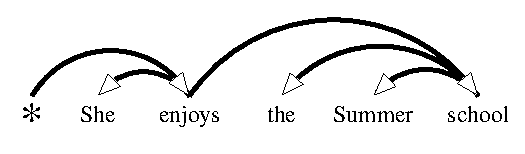
\includegraphics[width=0.6\columnwidth]{figs/parsing/example_proj}
\caption{A dependency tree for the sentence \emph{She enjoys the Summer school}. Note the additional dummy root symbol (*) which is included for convenience.}
\label{fig:deptree_proj}
\end{figure}


\subsection{Projective and Non-projective Parsing}

Dependency trees constructed using the method just described (\emph{i.e.}, lexicalization of context-free phrase-based trees) always satisfy the following properties: 
\begin{enumerate}
\item Each word (excluding the dummy root symbol) has exactly one parent. 
\item The dummy root symbol has no parents.
\item There are no cycles. 
\item The dummy root symbol has exactly one child. 
\item All arcs are \emph{projective}. This means that for any arc $\langle h,m \rangle$, all words in its span (\emph{i.e.}, all words lying between $h$ and $m$) 
are descendents from $h$ (i.e. there is a directed path of dependency links from $h$ to such word). 
\end{enumerate}

Conditions 1--3 ensure that the set of dependency links form a well-formed tree, rooted in the dummy symbol, which spans all the words of the sentence. 
Condition 4 requires that there is a single link departing from the root. 
Finally, a tree satisfying condition 5 is said \emph{projective}: it implies that arcs cannot cross (\emph{e.g.}, we cannot have arcs $\langle h,m \rangle$ and $\langle h',m' \rangle$ 
such that the word positions are ordered as $h < h' < m < m'$). 

In many languages (\emph{e.g.}, those which have free-order) we would like to relax the assumption that all trees must be projective. Even in languages which have fixed word order 
(such as English) there are syntactic phenomena which are awkward to characterize using projective trees arising from the context-free assumption. Usually, 
such phenomena are characterized with additional linguistic artifacts (e.g., traces, Wh-movement, \emph{etc.}). 
An example is the sentence (extracted from the Penn Treebank)
\begin{quote}
We learned a lesson in 1987 about volatility. 
\end{quote}
There, the prepositional phrase \emph{in 1987} should be attached to the verb phrase headed by \emph{learned} (since this is \emph{when} we learned the lesson), 
but the other prepositional phrase \emph{about volatility} should be attached to the noun phrase headed by \emph{lesson} (since the \emph{lesson} was about volatility). 
To explain such phenomenon, 
context-free grammars need to use additional machinery which allows words to be scrambled (in this case, via a movement transformation and the consequent insertion of a trace).
In the dependency-based formalism, we can get rid of all those artifacts altogether by allowing \emph{non-projective} parse trees. 
These are trees that satisfy conditions 1--3 above, but not necessarily conditions 4 or 5.%
\footnote{It is also common to impose conditions 1--4, in which case the tree need not be projective, but it must have a 
single link departing from the root. The algorithms to be described below can be adapted for this case.} 
The dependency tree in Fig.~\ref{fig:deptree_nonproj} is non-projective: note that the arc $\langle lesson, about \rangle$ is not projective. 

\begin{figure}
\begin{center}
    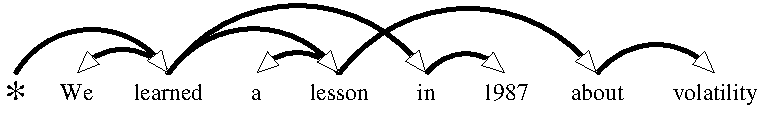
\includegraphics[width=1\columnwidth]{figs/parsing/example_nonproj}
  \caption{A non-projective parse tree.}
  \label{fig:deptree_nonproj}
  \end{center}
\end{figure}

We end this section by mentioning that dependency trees can have their arcs labeled, to provide more detailed syntactic information. 
For example, the arc $\langle enjoys, She \rangle$ could be labeled as {\tt SUBJ} to denote that the modifier \emph{She} has a subject function, and 
the arc $\langle enjoys, school \rangle$ could be labeled as {\tt OBJ} to denote that the modifier \emph{school} has an object function. 
For simplicity, we resort to \emph{unlabeled} trees, which just convey the backbone structure. To cope with the labels, one can use either a joint model 
that infers the backbone and labels altogether, or to have a two-stage approach that first gets the backbone structure, and then the arc labels. 

\subsection{Algorithms for Projective Dependency Parsing}

We now turn our attention to \emph{algorithms} for obtaining a dependency parse tree. 
We start by considering a simple kind of models which are called \emph{arc-factored}.  
These models assign a score $s_{\boldsymbol{\theta}}(h,m)$ to each possible arc $\langle h,m \rangle$ connecting a pair of words; 
they then score a particular dependency tree $t$ by summing over the individual scores of the arcs that are present in the tree: 
$$\mathrm{score}_{\boldsymbol{\theta}}(t) = \sum_{\langle h,m \rangle \in t} s_{\boldsymbol{\theta}}(h,m).$$ 
As usual, from the point of view of the parsing algorithm, 
it does not matter whether the scores come from a generative or discriminative approach, and which features were used to compute the scores. 
The three important inference tasks are: 
\begin{enumerate}
\item Obtain the tree with the largest score, 
$${\hat t} = \argmax_t \mathrm{score}_{\boldsymbol{\theta}}(t).$$
\item Compute the partition function (for a log-linear model),
$$Z(\mathbf{s_{\boldsymbol{\theta}}}) = \sum_t \exp(\mathrm{score}_{\boldsymbol{\theta}}(t)),$$
where $\mathbf{s_{\boldsymbol{\theta}}}$ is short-hand notation for the set of all the $s_{\boldsymbol{\theta}}( h,m )$ coefficients.
\item Compute the posterior marginals for all the possible arcs (which for a log-linear model is the gradient of the log-partition function), 
$$P_{\boldsymbol{\theta}}(\langle h,m \rangle \in t) = \frac{\partial \log Z(\mathbf{s_{\boldsymbol{\theta}}})}{\partial s_{\boldsymbol{\theta}}( h,m )}.$$
\end{enumerate}

%% \todo{Skip this exercise and write down an optional one at the end asking to implement
%% Eisner's algorithm given some pseudo-code and evaluate it on English data.}
%% \begin{exercise}
%% \textbf{(Warning: this exercise is somewhat complex. Feel free to think about it after the lab and ask your questions later!)}
%% In \emph{projective} dependency parsing using arc-factored models, the three tasks above can be solved in time $O(N^3)$. 
%% Sketch how the most likely dependency tree can be computed by ``adapting'' the CKY algorithm. 
%% (Hint: note that the CKY algorithm builds larger spans by combining smaller spans, 
%% and multiplies their weights by the weight of the corresponding production rule. 
%% In dependency parsing, each ``span'' is not represented by a constituent, 
%% but rather by the position of its lexical head. 
%% Convince yourself that this can only be either the leftmost or the rightmost position, 
%% and work out how the two spans can be combined.)
%% 
%% The instantiation of the CKY algorithm for projective dependency parsing is called Eisner's algorithm \citep{Eisner1996}. 
%% Analogously,  the partition function and the posterior marginals can be computed by 
%% adapting the inside-outside algorithm. 
%% \end{exercise}

As explained in this morning's lecture, 
in \emph{projective} dependency parsing using arc-factored models, the three tasks above can be solved in time $O(N^3)$, 
through Eisner's algorithm \citep{Eisner1996}, which is represented 
as Algorithm~\ref{alg:eisner}. 
Eisner's algorithm is related with the CKY algorithm in the sense that it also parses a sentence in a bottom-up 
fashion, building larger spans from smaller spans. 
In fact, the CKY algorithm can be adapted in a na\"ive manner to perform 
projective dependency parsing by dropping the constituent symbols and 
keeping track of the head positions of each span. This na\"ive strategy, however, would force us to 
manipulate five indices when combining two spans to form a larger span (the start and end points of the large span, 
the mid point, and the head positions for the two spans being combined), which would increase the 
complexity of the algorithm to $O(N^5)$. 
Eisner's algorithm uses the notion of \emph{complete} and \emph{incomplete} spans (in which all the right modifiers 
and all the left modifiers of a given head are all built separately) to reduce the complexity back to 
$O(N^3)$.
By replacing maximizations with summations, the same dynamic programming algorithm can be used to compute 
the partition function and the posterior marginals. 

\begin{algorithm}[h!]
   \caption{Eisner's algorithm for first-order projective dependency parsing\label{alg:eisner}}
\begin{algorithmic}[1]
   \STATE {\bfseries input:} Arc scores $s_{\boldsymbol{\theta}}(h,m)$, for $h \in \{0,\ldots,N\}$, 
   $m \in \{1,\ldots,N\}$, and $h \ne m$, associated with a sentence $s=w_1\ldots w_N$.
   \STATE \COMMENT{Initialization}
	\FOR{$i=0$ {\bfseries to} $N$}
	\STATE \COMMENT{Initialize incomplete spans.}
	\STATE $\mathrm{incomplete}[i,i,\leftarrow] := 0.0$
	\STATE $\mathrm{incomplete}[i,i,\rightarrow] := 0.0$
	\STATE
	\STATE \COMMENT{Initialize complete spans.}
	\STATE $\mathrm{complete}[i,i,\leftarrow] := 0.0$
	\STATE $\mathrm{complete}[i,i,\rightarrow] := 0.0$
	\ENDFOR
	\STATE
	\STATE \COMMENT{Induction}
	\FOR[$k$ is length of span]{$k=1$ {\bfseries to} $N$} 
	\FOR[$s$ is start of span]{$s=0$ {\bfseries to} $N-k$}
	\STATE Set $t := s + k$ \COMMENT{$t$ is end of span}
	\STATE
	\STATE \COMMENT{First, create incomplete spans.}
	\STATE $\mathrm{incomplete}[s,t,\leftarrow] := \max_{s \le r < t} (\mathrm{complete}[s,r,\rightarrow] + \mathrm{complete}[r+1,t,\leftarrow] + s_{\boldsymbol{\theta}}(t,s)) $
	\STATE $\mathrm{incomplete}[s,t,\rightarrow] := \max_{s \le r < t} (\mathrm{complete}[s,r,\rightarrow] + \mathrm{complete}[r+1,t,\leftarrow] + s_{\boldsymbol{\theta}}(s,t))$
	\STATE
	\STATE \COMMENT{Then, create complete spans.}
	\STATE $\mathrm{complete}[s,t,\leftarrow] := \max_{s \le r < t} (\mathrm{complete}[s,r,\leftarrow] + \mathrm{incomplete}[r,t,\leftarrow])$
	\STATE $\mathrm{complete}[s,t,\rightarrow] := \max_{s \le r < t} (\mathrm{incomplete}[s,r+1,\rightarrow] + \mathrm{complete}[r+1,t,\rightarrow])$
	\ENDFOR
	\ENDFOR
	\STATE
	\STATE \COMMENT{Termination}
	\STATE Backtrack to obtain the actual tree, whose score is $\mathrm{complete}[0,N,\rightarrow]$.
\end{algorithmic}
\end{algorithm}


\subsection{Algorithms for Non-Projective Dependency Parsing}

We turn our attention to \emph{non-projective} dependency parsing. In that case, efficient solutions also exist for the three problems above; 
interestingly, they are based in combinatorial algorithms which are not related at all with dynamic programming: 
\begin{itemize}
\item The first problem corresponds to finding the \emph{maximum weighted directed spanning tree} in a directed graph. 
This problem is well known in combinatorics and can be solved in $O(N^3)$ using Chu-Liu-Edmonds' algorithm 
\citep{Chu1965,Edmonds1967}.%
\footnote{There is a asymptotically faster algorithm by \citet{Tarjan1977} which solves the same problem in $O(N^2)$.} %
This has first been noted by \citet{McDonald2005b}. 
\item The second and third problems can be solved by invoking another important result in combinatorics, the 
\emph{matrix-tree theorem} \citep{Tutte1984}. This fact has been noticed independently by 
\citet{DSmithSmith2007,Koo2007,McDonald2007}. The cost is that of computing a determinant and inverting a matrix, 
which can be done in time $O(N^3)$. 
The procedure is as follows. 
We first consider the directed weighted graph formed by including all 
the possible dependency links $\langle h,m \rangle$ (including the ones departing from the dummy root symbol, 
for which $h = 0$ by convention), along with weights 
given by $\exp(s_{\boldsymbol{\theta}}(h,m))$, 
and compute its 
$(N+1)$-by-$(N+1)$ Laplacian matrix $\boldsymbol{L}$ whose entries are:
\begin{equation}
L_{hm} = \left\{ 
\begin{array}{ll}
\sum_{h'=0}^N\exp(s_{\boldsymbol{\theta}}(h',m)), & \text{if $h=m$,} \\
-\exp(s_{\boldsymbol{\theta}}(h,m))), & \text{otherwise.}
\end{array}\right.
\end{equation}
%Denote by $\boldsymbol{r}=(r_m)_{m=1,\ldots,n}$ the first row of this matrix, transposed, with the first entry removed, i.e., 
%$r_i \triangleq -\exp(s_{\boldsymbol{\theta}}(0,m)))$.
%Furthermore,
Denote by $\hat{L}$ the $(0,0)$-minor of $L$, 
\emph{i.e.}, the matrix obtained from $L$ 
by removing the first row and column. Consider its determinant $\det \hat{L}$ and its 
inverse $\hat{L}^{-1}$. %
Then: %
%% \footnote{The above described is the \emph{multiple root} case, where a valid dependency tree may have multiple words 
%% attached to the dummy root; there is also a solution for 
%% the single root case, where only one effective root is permitted; see \citet{Koo2007}.} %
\begin{itemize}
\item the partition function is given by 
\begin{equation}
Z(\mathbf{s_{\boldsymbol{\theta}}}) = \det \hat{L};
\end{equation}
\item the posterior marginals 
are given by 
\begin{equation}
P_{\boldsymbol{\theta}}(\langle h,m \rangle \in t) = \left\{
\begin{array}{ll}
\exp(s_{\boldsymbol{\theta}}(h,m))\cdot([\hat{L}^{-1}]_{mm} - 
[\hat{L}^{-1}]_{mh}) & \text{if $h \ne 0$}\\
\exp(s_{\boldsymbol{\theta}}(0,m))\cdot[\hat{L}^{-1}]_{mm} & \text{otherwise.}
\end{array}
\right.
\end{equation}
%% $P_{\boldsymbol{\theta}}(\langle h,m \rangle \in t) = 
%% \exp(s_{\boldsymbol{\theta}}(h,m))\cdot([\hat{L}^{-1}]_{mm} - 
%% [\hat{L}^{-1}]_{mh})$, for $h \ne 0$, and 
%% $P_{\boldsymbol{\theta}}(\langle 0,m \rangle \in t) = \exp(s_{\boldsymbol{\theta}}(0,m))\cdot[\hat{L}^{-1}]_{mm}$.
\end{itemize}
\end{itemize}

\begin{exercise}
In this exercise you are going to experiment with arc-factored non-projective dependency parsers. 

The CoNLL-X and CoNLL 2008 shared task datasets \citep{conll06st,Surdeanu2008} contain 
dependency treebanks for $14$ languages. 
In this lab, we are going to experiment with the Portuguese and English datasets. 
We preprocessed those datasets to exclude all sentences with more than 
$15$ words; this yielded the files:
\begin{itemize}
\item {\tt data/deppars/portuguese\_train.conll},
\item {\tt data/deppars/portuguese\_test.conll},
\item {\tt data/deppars/english\_train.conll},
\item {\tt data/deppars/english\_test.conll}.
\end{itemize}

\begin{enumerate}
\item After importing all the necessary libraries, load the Portuguese dataset: 
\begin{python}
import sys
sys.path.append('.' )

import lxmls.parsing.dependency_parser as depp

dp = depp.DependencyParser()
dp.read_data("portuguese")
\end{python}
Observe the statistics which are shown. How many features are there in total?

\item We will now have a close look on the \emph{features} that can be used in the parser. 
Examine the file:
\begin{quote}
{\tt lxmls/parsing/dependency\_features.py}. 
\end{quote}
The following method takes a sentence and computes a vector of features for each possible arc $\langle h, m \rangle$: 
\begin{python}
def create_arc_features(self, instance, h, m, add=False):
	'''Creates features for arc h-->m.'''
\end{python}
We grouped the features in several subsets, so that we can conduct some ablation experiments: 
\begin{itemize}
\item \emph{Basic} features that look only at the parts-of-speech of the words that can be connected by an arc;
\item \emph{Lexical} features that also look at these words themselves;
\item \emph{Distance} features that look at the length and direction of the dependency link (\emph{i.e.}, distance between the two words);
\item \emph{Contextual} features that look at the context (part-of-speech tags) of the words 
surrounding $h$ and $m$. 
\end{itemize}
In the default configuration, only the basic features are enabled. The total number of features 
is the quantity observed in the previous question. 
With this configuration, 
train the parser by running $10$ epochs of the structured perceptron algorithm: 
\begin{python}
dp.train_perceptron(10)
dp.test()
\end{python}
What is the accuracy obtained in the test set? (Note: the shown accuracy is the fraction of words whose parent was correctly predicted.)\\
% {\emph{Ans}: I obtained an accuracy of 49.52\% for 109 test instances (142 features) (so para ajudar nos labs)}
\item Repeat the previous exercise by 
subsequently enabling the lexical, distance and contextual features:
\begin{python}
dp.features.use_lexical = True
dp.read_data("portuguese")
dp.train_perceptron(10)
dp.test()

dp.features.use_distance = True
dp.read_data("portuguese")
dp.train_perceptron(10)
dp.test()

dp.features.use_contextual = True
dp.read_data("portuguese")
dp.train_perceptron(10)
dp.test()
\end{python}
For each configuration, write down the number of features and test set accuracies. 
Observe the improvements obtained when more features were added.\\
% {\emph{Ans}: Lexical features: accuracy of 57.66\% (46216 features).\\
% Distance features: accuracy of 71.46\% (46224 features).\\
% Contextual features: accuracy of 87.45\% (92918 features).\\
% for 109 test instances (so para ajudar nos labs)}\\
Feel free to engineer new features!

\item Which of the three important inference tasks discussed above (computing the most likely tree, 
computing the partition function, and computing the marginals) need to be performed in the structured perceptron algorithm? 
What about a maximum entropy classifier, with stochastic gradient descent?  
Check your answers by looking at the following two methods in {\tt code/dependency\_parser.py}:\\
% {\emph{Ans}: structured perceptron is done with function \emph{parse\_nonproj} for computing Chu-Liu-Edmonds algorithm for computing the most likely tree.\\
% Maxent with CRF is done with function \emph{parse\_marginals\_nonproj} for computing marginals and the log-partition function using the matrix-tree theorem.}
\begin{python}
def train_perceptron(self, n_epochs):
...

def train_crf_sgd(self, n_epochs, sigma, eta0 = 0.001):
...
\end{python}
Repeat the last exercise by training a maximum entropy classifier, with stochastic gradient descent, 
using $\lambda = 0.01$ and a initial stepsize of $\eta_0 = 0.1$: 
\begin{python}
dp.train_crf_sgd(10, 0.01, 0.1)
dp.test()
\end{python}
Compare the results with those obtained by the perceptron algorithm.\\
%{\emph{Ans:}CRF\_SGD accuracy: 88.12\%.}

\item Train a parser for English using your favourite learning algorithm: 
\begin{python}
dp.read_data("english")
dp.train_perceptron(10)
dp.test()
\end{python}
%{\emph{Ans}: accuracy: 88.56\% for 338014 features and 509 test instances.}\\

The predicted trees are placed in the file {\tt data/deppars/english\_test.conll.pred}. 
To get a sense of which errors are being made, you can 
check the sentences that differ from the gold standard (see the data in {\tt data/deppars/english\_test.conll}) 
and visualize those sentences, \emph{e.g.}, in 
\url{http://brenocon.com/parseviz/}. 

\item (Optional.) Implement Eisner's algorithm for \emph{projective} dependency parsing. 
The pseudo-code is shown as Algorithm~\ref{alg:eisner}. Implement this algorithm as the function

\begin{python}
    def parse_proj(self, scores):
        '''
        Parse using Eisner's algorithm.
        '''
\end{python}
in file ${\tt{dependency\_decoder.py}}$. The input is a matrix of arc scores, whose dimension is 
$(N+1)$-by-$(N+1)$, and whose $(h,m)$ entry contains the score $s_{\boldsymbol{\theta}}(h,m)$. 
In particular, the first row contains the scores for the arcs that depart from the root, 
and the first column's values, along with the main diagonal, are to be ignored (since no arcs 
point to the root, and there are no self-pointing arcs).
To make your job easier, we provide an implementation of the backtracking part:
\begin{python}
    def backtrack_eisner(self, incomplete_backtrack, complete_backtrack, s, t, direction, complete, heads):
\end{python}
so you just need to build complete/incomplete spans and their backtrack pointers and then call
\begin{python}
    heads = -np.ones(N+1, dtype=int)
    self.backtrack_eisner(incomplete_backtrack, complete_backtrack, 0, N, 1, 1, heads)
    return heads
\end{python}
to obtain the final parse.

To test the algorithm, retrain the parser on the English data (where the trees are actually all
projective) by setting the flag ${\tt{dp.projective}}$ to ${\tt{True}}$:
\begin{python}
dp = depp.DependencyParser()
dp.features.use_lexical = True
dp.features.use_distance = True
dp.features.use_contextual = True
dp.read_data("english")
dp.projective = True
dp.train_perceptron(10)
dp.test()
\end{python}

You should get the following results:
\begin{python}
Number of sentences: 8044
Number of tokens: 80504
Number of words: 12202
Number of pos: 48
Number of features: 338014
Epoch 1
Training accuracy: 0.835637168541
Epoch 2
Training accuracy: 0.922426254687
Epoch 3
Training accuracy: 0.947621628947
Epoch 4
Training accuracy: 0.960326602521
Epoch 5
Training accuracy: 0.967689840538
Epoch 6
Training accuracy: 0.97263631025
Epoch 7
Training accuracy: 0.97619370285
Epoch 8
Training accuracy: 0.979209016579
Epoch 9
Training accuracy: 0.98127569228
Epoch 10
Training accuracy: 0.981320865519
Test accuracy (509 test instances): 0.886732599366
\end{python}

\end{enumerate}
\end{exercise}



\subsection{Model Refinements}

A number of refinements has been made that yield more accurate dependency parsers. We mention just a few: 
\begin{description}
\item[Sibling and grandparent features.] 
The arc-factored assumption fails to capture correlations between pairs of arcs. 
The dynamic programming algorithms for the \emph{projective} case can be extended (at some additional cost) to 
handle features that look at consecutive sibling arcs on the same side of the head 
(\emph{i.e.}, pairs of arcs of the form $\langle h,m \rangle$ and $\langle h,s \rangle$ 
with $h < m < s$ or $h > m > s$, such that no arc $\langle h,r \rangle$ exists with $r$ between $m$ and $s$. 
This has been done by \citet{Eisner1999}. Similarly, grandparents can also be accommodated 
with similar extensions \citep{Carreras2007}. These are called ``second-order models.''

For the non-projective case, however, any extension beyond the arc-factored model becomes NP-hard \citep{McDonald2007}. 
Yet, approximate algorithms have been proposed to handle ``second-order models'' that seem to work well: 
a greedy method \citep{McDonald2006CoNLL}, 
loopy belief propagation \citep{DSmith2008}, a linear programming relaxation \citep{Martins2009ACL}, 
and a dual decomposition method \citep{Koo2010EMNLP}. 
\item[Third-order models.]
For the projective case, third order models have also been considered \citep{Koo2010}. This was 
extended to the non-projective case by \citet{Martins2013ACL}.
\item[Transition-based parsers.]
Like in the phrase-based case, there is a totally different line of work which models parsers as a sequence of greedy 
shift-reduce decisions \citep{Nivre2006CoNLL,Huang2010}. These parsers seem to be very fast (expected linear time) 
and only slightly less accurate than 
the state-of-the-art. Solutions have been worked out for the non-projective case also \citep{Nivre2009}. 
\end{description}

\subsection{External Links}

If you want to check a demo of a parser that use some of the extensions above, you can do so 
at 
\begin{quote}
{\url{http://demo.ark.cs.cmu.edu/parse}} 
\end{quote}
This demo uses  
TurboParser ({\url{http://www.ark.cs.cmu.edu/TurboParser}}), a free software implementation of a fast and accurate dependency parser 
that can parse thousands of tokens per second with state-of-the-art accuracies 
(way faster than the Python implementation that you have used at the labs). 
Feel free to try it at home!

Other well-known software toolkits that implement dependency parsers are:
\begin{itemize}
\item MSTParser ({\url{http://www.seas.upenn.edu/~strctlrn/MSTParser/MSTParser.html}}), a graph-based dependency parser;
\item MaltParser ({\url{http://www.maltparser.org/}}), a transition-based parser;
\item DPO3 ({\url{http://groups.csail.mit.edu/nlp/dpo3/}}), a third-order projective parser;
\item Linear-time dynamic programming parser ({\url{http://acl.cs.qc.edu/~lhuang/}}), a fast transition-based parser.
\end{itemize}








%% \begin{figure}
%% \small
%% \begin{tabular}{ll}
%% (a) 
%% \Tree [.S [.NP [ She ].Pro ] [.VP [ enjoys ].V [.NP [ the ].Det [.Nbar [ Summer ].N [ school ].N ] ] ] ] &
%% (b) 
%% \Tree [.S~(\emph{enjoys}) [.NP~(\emph{she}) [ She ].Pro~(\emph{she}) ] [.VP~(\emph{enjoys}) [ enjoys ].V~(\emph{enjoys}) [.NP~(\emph{school}) [ the ].Det~(\emph{the}) [.Nbar~(\emph{school}) [ Summer ].N~(\emph{Summer}) [ school ].N~(\emph{school}) ] ] ] ] \\
%% (c)
%% \Tree [.enjoys [ ].she [.school [ ].the [ ].Summer ] ] &
%% (d)
%% \begin{tabular}{c}
%% \\
%% 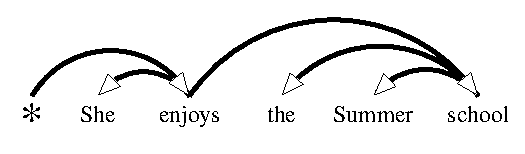
\includegraphics[width=0.55\columnwidth]{figs/parsing/example_proj}
%% \end{tabular}
%% \end{tabular}
%% \end{figure}


%\chapter{Unsupervised Learning}
%In this class we will address the problem of \emph{unsupervised} learning of linguistic structures, namely 
\emph{parts-of-speech}. 
In this setting we are not given any labeled data. Instead, all we get to see is a set of natural language sentences.  
The underlying question is: 

\begin{quote}
Can we learn something from raw text?
\end{quote}

This task is particularly challenging since the process by which linguistic structures are generated is not always clear 
and even when it is, it is normally too complex to be
formally expressed. Nevertheless, unsupervised learning has been applied to a
wide range of natural language processing tasks, such as: 
\pos\ Induction  \citep{schutze1995distributional,merialdo1994tet,clark03combining},
Dependency Grammar Induction \citep{klein2004acl,smith2006annealing}, Constituency Grammar Induction \citep{klein2004acl}, Statistical Word Alignments 
\citep{brown94mathematic} and Anaphora Resolution \citep{charniak2009works}, just to name a few. 

Different motivations have pushed research in this area. From both a linguistic and cognitive point of view, 
unsupervised learning is useful as a tool to study language acquisition. 
From a machine learning point of view, unsupervised learning is a fertile ground for testing new learning methods, 
where significant improvements can yet be made. 
From a more pragmatic perspective, unsupervised learning is required
since annotated corpora is a scarce resource for different reasons. Independently of the reason, unsupervised learning is an increasing active field of research.

A first problem with unsupervised learning, since we don't observe any labeled data (i.e., 
the training set is now $\mathcal{D} = \{x_1,\ldots, x_M\}$), 
is that most of the methods studied so far (Perceptron, Mira, SVMs) cannot be used since we cannot compare 
the true output with the predicted output. 
Note also that a direct minimization of the \emph{complete negative log-likelihood} of the data, $\log P_{\theta}(\mathcal{D})$, 
is very challenging, since it would require marginalizing out (\emph{i.e.}, summing over) all possible hidden variables:
\begin{equation}
 \log P_{\theta}(\mathcal{D}) =  \sum_{m=1}^M \log \sum_{y \in \mathcal{Y}} P_{\theta} (x_m,y).
\end{equation}
Note also that the objective above is \emph{non-convex} even for a linear model: hence, it may have local minima, which makes optimization much 
more difficult. 

Another observation is that normally we are restricted to generative models, 
with some remarkable exceptions~\citep{smith2005acl}, since the objective of discriminative models when no labels are observed are 
meaningless ($\sum_{y_m } P(y^m |x^m) = 1$); this rules out, for instance, Maximum Entropy classifiers.  

The most common optimization method in the presence of hidden (latent) variables is the Expectation Maximization (EM) algorithm. Note that this algorithm is a generic optimization routine that does not depend on a particular model. The next section will explain the EM algorithm. On Section \ref{posi} we will apply the EM algorithm to the task of part-of-speech induction, where one is given raw text and a number of clusters and the task is to cluster words that behave similarly in a grammatical sense. 

\section{\label{em}Expectation Maximization Algorithm}
Given a particular model $\joint$ and a training corpus $\X$ of $D$ sentences $\sent^1 \ldots \sent^D$, training 
seeks model parameters $\theta$ that minimize the negative log-likelihood of the corpus:
\begin{equation}
\label{loglikelihoood}
\mathbf{Negative\;Log\;Likelihood\!:}\;\;\;\; \likelihood(\theta) =\XpD [-\log \marginal] = \XpD [-\log \sum_{\hseq} \joint],
\end{equation}
where $\XpD [f(\sent)] = \frac{1}{D}\sum_{i=1}^{D} f(\sent^i)$ denotes the empirical average of a function $f$ over the training corpus.

Because of the hidden variables $\hseq$, the likelihood term contains a
sum over all possible hidden structures inside of a logarithm, which
makes this quantity hard to compute.

The most common minimization
algorithm to fit the model parameters in the presence of hidden
variables is the Expectation Maximization (EM) algorithm. 

The EM procedure can be thought of intuitively in the following way. 
If we observe the hidden variables' values for all sentences in the
corpus, then we could easily compute the maximum likelihood value of
the parameters as described in Section \ref{ml}. 
On the other hand, if we had the model parameters we could label data
using the model, and collect the
sufficient statistics described in Section \ref{ml}.
Since we are working in an unsupervised setting, we never get to
observe the hidden state sequence. Instead, given a 
training set $\X = \{\sent^1 \ldots \sent^D\}$, we will need to
collect sufficient statistics, or expected counts that
represent the expected number of times that each hidden variable is
expected to be used with the current parameters setting. These sufficient
statistics will then be used during learning as fake observations of
the hidden variables. Using the node and edge posterior distributions
described in Equations \ref{eq::nodePosterior} and \ref{eq::edgePosterior},
the sufficient statistics can 
be computed by the following formulas:
\begin{align}
\mathbf{Initial \ Counts\!:}\;\;\;\;  &  ic(\hv_l) = \sum_{d=1}^D
\gamma_1 (\hv_l); \label{eq::initialCountsPost}\\
\mathbf{Final \ Counts\!:}\;\;\;\;  &  fc(\hv_N,\hv _{N-1}) = \sum_{d=1}^D  \xi_{N-1} (\hv_l,\hv_m); \label{eq::finalCountsPost}\\
\mathbf{Transition \ Counts\!:}\;\;\;\;  &  tc(\hv_l,\hv _m) = \sum_{d=1}^D \sum_{i = 1}^{N-1}  \xi_i (\hv_l,\hv_m); \label{eq::transitionCountsPost}\\
\mathbf{State \ Counts\!:}\;\;\;\;  &  sc(\vv_q,\hv_m) = \sum_{d=1}^D \sum_{i = 1 , \obs_i = \vv_q }^{N}  \gamma_i (\hv_m). \label{eq::stateCountsPost}
\end{align}

Compare the previous Equations with the ones described in Section
\ref{ml} for the same quantities. The main difference is that while in
the presence of supervised data you sum the observed events, when you
have no label data you sum the posterior probabilities of each
event. If these probabilities were such that the probability mass was
around single events then both Equations will produce the same result.



The EM procedure starts with an initial guess for the parameters
$\theta^0$ at time $t = 0$. The algorithm iterates for $T$ iterations
until it converges to a local minima of the negative log likelihood, and each
iteration is divided into two steps:

\begin{description} 
 \item The first step - ``E Step'' (Expectation) - 
computes the posteriors for the hidden variables
$\posterior$, given the current parameter values $\theta^t$ and the observed variables. 
In the case of the HMM this requires only to run the FB algorithm.
\item The second step - ``M step'' (Maximization) - uses $\posterior$ to
``softly fill in'' the values of the hidden variables $\hseq$, and
collects the sufficient statistics, initial counts (Eq: \ref{eq::initialCountsPost}), transition counts (Eq:
\ref{eq::transitionCountsPost}) 
and state counts (Eq: \ref{eq::stateCountsPost}) and uses those
counts to estimate maximum likelihood parameters $\theta^{t+1}$ as described in
Section \ref{ml}.
\end{description}

The EM algorithm is guaranteed to
converge to a local minimum of $\likelihood(\theta)$ under mild
conditions.  
Note that we are not committing to the best assignment of the hidden variables, but
summing the occurrences of each parameter weighed by the posterior
probability of all possible assignments. 
This modular split into two intuitive and straightforward steps
accounts for the vast popularity of EM.

More formally, EM minimizes $\likelihood(\theta)$ via block-coordinate descent on an upper bound $F(q,\theta)$ using an auxiliary distribution over the latent variables
$\auxq$:
\begin{eqnarray}
\likelihood(\theta)  &=& \XpD \left[-\log \sum_{\hseq}\joint \right]\\
\label{eq:jensen}&=& \XpD \left[-\log \sum_{\hseq}
\auxq*\frac{\joint}{\auxq}\right] \le \XpD \left[- \sum_{\hseq} \auxq\log \frac{\joint}{\auxq}\right] \\
&=& \XpD \left[\sum_{\hseq} \auxq\log \frac{\auxq}{\joint}\right] =  F(q,\theta),
\end{eqnarray}
where we have multiplied and divided the $\joint$ by the same quantity
$\auxq$, and 
the lower bound comes from applying Jensen Inequality (Equation
\ref{eq:jensen}). $F(q,\theta)$ is normally referred to as the energy
function, which comes from the physics field and refers to the energy of a given system that we want to minimize.
\begin{equation}
\mathbf{EM\;Upper\;Bound\!:}\;\;\;\;\;\likelihood(\theta) \le F(q,\theta) =
\XpD \left[\sum_{\hseq} \auxq\log \frac{\auxq}{\joint}\right].
\end{equation}
The alternating E and M steps at iteration $t+1$ can be seen as minimizing the energy function first 
with respect to $\auxq$ and then with respect to $\theta$:
\begin{eqnarray}
\hspace{-5mm}{\mathbf E\!:}&& q^{t+1}(\hseq\mid\sent) =
\argmin_{\auxq} F(q,\theta^t)
  = \argmin_{\auxq} \KL(q(\hseq\mid\sent)\,||\,p_{\theta^t}(\hseq\mid\sent)) = p_{\theta^t}(\hseq\mid\sent);
 \label{eq:e-step} \\
\hspace{-5mm}{\mathbf M\!:}&& \theta^{t+1} = \argmin_\theta
F(q^{t+1},\theta) = \argmax_\theta \XpD\!\left[\sum_{\hseq}
q^{t+1}(\hseq\mid\sent)\log p_\theta(\sent,\hseq)\right];
\label{eq:m-step}
\end{eqnarray}
where $\KL(q||p) = \Xp_q[\log \frac{q(\cdot)}{p(\cdot)}]$ is the
Kullback-Leibler divergence. The KL term in the E-Step results from 
dropping all terms from the energy function that are constant for a
set $\theta$, in this case the likelihood of the observation sequence
$\marginal$:

\begin{align}
\sum_{\hseq} \auxq\log \frac{\auxq}{\joint} &= \sum_{\hseq} \auxq\log
\auxq - \sum_{\hseq} \auxq\log \joint  \\ 
&= \sum_{\hseq} \auxq\log \auxq - \sum_{\hseq} \auxq\log \marginal
\posterior \\
&= \sum_{\hseq} \auxq\log \frac{\auxq}{\posterior} - \log \marginal \\
&= \KL(\auxq||\posterior) - \log \marginal.
\end{align}

Algorithm ~\ref{alg::em} presents the pseudo code for the EM
algorithm. Note that this algorithm is agnostic of a particular model,
it only requires the model to implement a common interface.

\begin{algorithm}
\begin{algorithmic}[1]
  \STATE {\bfseries input:} dataset $\mathcal{D}$, an initialized model
    \FOR{$t = 1$ {\bfseries to} $T$}
      \STATE model.clear\_counts()
      \FOR{$seq \in \mathcal{D}$}
        \STATE \textbf{E-Step:}
        \STATE posteriors,likelihood =model.compute\_posteriors($seq$)
        \STATE model.update\_counts($seq$,posteriors)
      \ENDFOR
      \STATE \textbf{M-Step:}
         \STATE model.update\_params(counts)
    \ENDFOR
\end{algorithmic}    
\caption[EM algorithm]{\label{alg::em}  EM algorithm.} 
\end{algorithm}


One important thing to note in Algorithm \ref{alg::em} is that for the
HMM model we already have all the model pieces we require. In fact
the only method we don't have yet implemented from previous classes is
the method to update\_counts(posteriors). 

\begin{exercise}

Implement the method update\_counts(seq,posteriors).
\begin{python}
 def update_counts(self,seq,posteriors):
\end{python}

Use the method you defined previously to check the count tables to
check if this method is correct. Use a corpus with only one sentence
to make the test simpler.

\begin{python}
In []: run readers/pos_corpus.py
In []: posc = PostagCorpus("en",max_sent_len=15,train_sents=1,dev_sents=0,test_sents=0)
In []: run sequences/hmm.py
In []: hmm = HMM(posc)
In []: hmm.train_supervised(posc.train,smoothing=0.1)
In []: hmm.clear_counts()
In []: posteriors,likelihood = hmm.get_posteriors(posc.train.seq_list[0])
In []: hmm.update_counts(posc.train.seq_list[0],posteriors)
In []: hmm.sanity_check_counts(posc.train)
\end{python}

If you pass this test, then you have all the pieces to implement the
EM algorithm. Look at the code for EM algorithm in file
\emph{sequences/em.py} and check it for yourself. 

\begin{python}
    def train(self,seq_list,nr_iter=10,smoothing=0,evaluate=True):
        if(evaluate):
            ### Evaluate accuracy at initial iteration
            pred = self.model.viterbi_decode_corpus(seq_list.seq_list)
            acc = self.model.evaluate_corpus(seq_list.seq_list,pred)
        for t in xrange(1,nr_iter):
            #E-Step
            total_likelihood = 0
            self.model.clear_counts(smoothing)
            for seq in seq_list.seq_list:
                posteriors,likelihood = self.model.get_posteriors(seq)
                self.model.update_counts(seq,posteriors)
                total_likelihood += likelihood
            print "Iter: %i - Log Likelihood %f"%(t,-1*math.log(total_likelihood))
            #M-Step
            self.model.update_params()

            if(evaluate):
                 ### Evaluate accuracy at this iteration
                pred = self.model.viterbi_decode_corpus(seq_list.seq_list)
                acc = self.model.evaluate_corpus(seq_list.seq_list,pred)
                print "Iter: %i acc %f"%(t,acc)
\end{python}

\end{exercise}

%%% Local Variables: 
%%% mode: latex
%%% TeX-master: "../../guide"
%%% End: 


\section{\label{posi}Part of Speech Induction}
In this section we present the \posi\ task. \pos\ tags are pre-requisite for many text applications. The task of \pos\ tagging where one is given a labeled training set of words and respective tags is a well studied task with several methods achieving high prediction quality, as we saw in Chapters \ref{day:seq} and \ref{day:seq_disc}. 

On the other hand the task of \posi\ where one does not have access to a labeled corpus is a much harder task with a huge space for improvement. In this case, we are given only the raw text along with sentence boundaries and a predefined number of clusters we can use. This problem can be seen as a clustering problem. We want to cluster words that behave grammatically in the same way on the same cluster. This is a much harder problem.

Formally, the problem setting is the following: we are given a training set $\X = \sent^1 \ldots \sent^D$ of $D$ training examples, where each example $\sent = \obs_1 \ldots \obs_N$ is a sentence of $N$ words, whose values $\vv$ are taken from a vocabulary $\vocab$ of possible word types. We are also given the set of clusters $\hvocab$ that we are allowed to use. The hidden structure $\hseq = \hs_1 \ldots \hs_N$ corresponds to a sequence of cluster assignments for each individual word, such that $\hs_n = \hv_l$ with $\hv_l \in \hvocab$. 

Depending on the task at hand we can pick an arbitrary number of clusters. If the goal is to test how well our method can recover the true pos tags then we should use the same number of clusters as pos tags. On the other hand, if the task is to extract features to be used by other methods we can use a much bigger number of clusters (e.g. 200) to capture correlations not captured by pos tags, like lexical affinity. 

Note, however that nothing is said about the identity of each cluster. The model has no preference in assigning cluster 1 to nouns vs cluster 2 to nouns. Given this non-identifiability several metrics have been proposed for evaluation \citep{Reichart09,haghighi2006naacl,Meila07,RosenbergH07}. In this class we will use a common and simple metric called \textbf{1-Many}, which maps each cluster to majority pos tag that it contains (see Figure \ref{fig:cm_uns} for an example). 

\begin{figure}
\centering
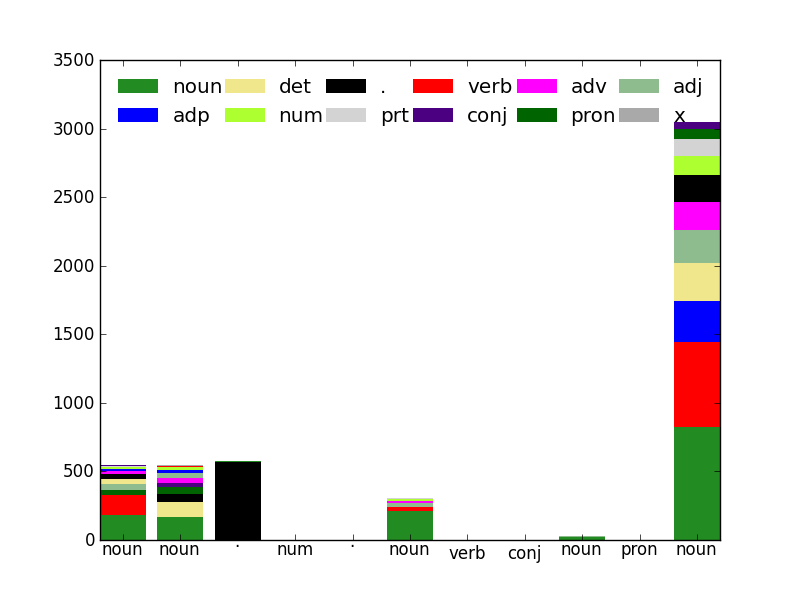
\includegraphics[scale=.5]{figs/sequences/cm_uns1.png}
\caption{\label{fig:cm_uns} Confusion Matrix example. Each cluster is a column. The best tag in each column is represented under the column (1-many) mapping. Each color represents a true Pos Tag.}
\end{figure}


\begin{exercise}
Run the EM algorithm for part of speech induction:
\begin{python}
In []: run readers/pos_corpus.py
In []: posc = PostagCorpus("en",max_sent_len=15,train_sents=1000,dev_sents=0,test_sents=0)
In []: run sequences/hmm.py
In []: hmm = HMM(posc)
In []: hmm.initialize_radom()
In []: run sequences/em.py
In []: em = EM(posc,hmm)
In []: em.train(posc.train,nr_iter=20)
Out []: Init acc 0.335505
Out []: Iter: 1 - Log Likelihood 16.071708
Out []: Iter: 1 acc 0.361960
Out []: Iter: 2 - Log Likelihood 11.212829
Out []: Iter: 2 acc 0.381000
Out []: Iter: 3 - Log Likelihood 11.091918
Out []: Iter: 3 acc 0.387013
Out []: Iter: 4 - Log Likelihood 10.751445
Out []: Iter: 4 acc 0.391222
Out []: Iter: 5 - Log Likelihood 10.046576
Out []: Iter: 5 acc 0.390420
Out []: Iter: 6 - Log Likelihood 9.055178
Out []: Iter: 6 acc 0.391723
Out []: Iter: 7 - Log Likelihood 8.109925
Out []: Iter: 7 acc 0.390420
Out []: Iter: 8 - Log Likelihood 7.497388
Out []: Iter: 8 acc 0.390520
Out []: Iter: 9 - Log Likelihood 7.225907
Out []: Iter: 9 acc 0.393827
Out []: Iter: 10 - Log Likelihood 7.127711
Out []: Iter: 10 acc 0.398236
Out []: Iter: 11 - Log Likelihood 7.105954
Out []: Iter: 11 acc 0.404449
Out []: Iter: 12 - Log Likelihood 7.111193
Out []: Iter: 12 acc 0.406654
Out []: Iter: 13 - Log Likelihood 7.041794
Out []: Iter: 13 acc 0.411264
Out []: Iter: 14 - Log Likelihood 6.958736
Out []: Iter: 14 acc 0.408558
Out []: Iter: 15 - Log Likelihood 6.828692
Out []: Iter: 15 acc 0.407656
Out []: Iter: 16 - Log Likelihood 6.693052
Out []: Iter: 16 acc 0.403848
Out []: Iter: 17 - Log Likelihood 6.670297
Out []: Iter: 17 acc 0.405451
Out []: Iter: 18 - Log Likelihood 6.684892
Out []: Iter: 18 acc 0.408658
Out []: Iter: 19 - Log Likelihood 6.706640
Out []: Iter: 19 acc 0.412166
\end{python}
Note: your results may not be the same as in this example since we are using a random start, but the trend should be the same. Also note that in some iterations the likelihood does not go down because of some rounding errors, however the general trend is that likelihood decreases over iterations. 
\end{exercise}

In the previous exercise we used an HMM to do Part-of-Speech induction using 12 clusters (by omission the HMM uses as number of hidden states the one provided by the corpus). A first observation is that the log-likelihood is always increasing as expected. Another observation is that the accuracy goes up from 33\% to 41\%. Note that normally you will run this algorithm for 200 iterations, we stopped earlier for time constraints. Another observations is that the accuracy is not monotonic increasing, this is because the likelihood is not a perfect proxy for the accuracy. In fact all that likelihood is measuring are co-occurrences of words in the corpus; it has no idea of pos tags. The fact we are improving derives from the fact that language is not random but follows some specific hidden patterns. In fact this patterns are what true pos-tags try to capture. A final observation is that the performance is really bad compared to the supervised scenario, so there is a lot of space for improvement. The actual state of the art is around 71\% for fully unsupervised~\citep{JoaoThesis,bergkirkpatrick2010naacl} and 80\% \citep{das-petrov:2011:ACL-HLT2011} using parallel data and information from labels in the other language. 

Looking at Figure \ref{fig:cm_uns} shows the confusion matrix for this particular example. 
A first observation is that most clusters are mapped to nouns, verbs or punctuation. 
This is a none fact since there are many more nouns and verbs than any other tags. Since maximum likelihood prefers probabilities 
to be uniform (Imagine two parameters. In one setting both have value 0.5 so the likelihood will be 0.5*0.5 = 0.25, 
while in the other case one as 0.1 and 0.9 so the maximum likelihood is 0.09). Several approaches have been proposed to 
address this problem under moving towards a Bayesian setting or using 
Posterior Regularization \citep{johnson2007dtf,graca2009nips} more about this later today. 
Part-of-Speech induction is a very active field of research, in fact in the last two ACL conferences (Association for Computational Linguistics) the short paper award (2010) and the best paper award (2011) were about this topic~\citep{lamar-EtAl:2010:Short,das-petrov:2011:ACL-HLT2011}.


% \begin{exercise}

% Repeat the previous exercise using a different number of hidden states (20,50). Note that the higher the number of states is the slower the training will be.
% What do you observe? Look at the confusion matrix and try to explaing what is happening.

% \begin{python}
% In []: run readers/pos_corpus.py
% In []: posc = PostagCorpus("en",max_sent_len=15,train_sents=1000,dev_sents=0,test_sents=0)
% In []: run sequences/hmm.py
% In []: hmm = HMM(posc,nr_states=20)
% In []: hmm.initialize_radom()
% In []: run sequences/em.py
% In []: em = EM(posc,hmm)
% In []: em.train(posc.train,nr_iter=20)
% Init acc 0.348933
% Iter: 1 Negative Log Likelihood 16.038424
% Iter: 1 acc 0.362662
% Iter: 2 Negative Log Likelihood 11.200816
% Iter: 2 acc 0.370177
% Iter: 3 Negative Log Likelihood 11.046597
% Iter: 3 acc 0.380800
% Iter: 4 Negative Log Likelihood 10.607496
% Iter: 4 acc 0.389518
% Iter: 5 Negative Log Likelihood 9.809817
% Iter: 5 acc 0.394027
% Iter: 6 Negative Log Likelihood 8.949717
% Iter: 6 acc 0.396733
% Iter: 7 Negative Log Likelihood 8.105404
% Iter: 7 acc 0.398337
% Iter: 8 Negative Log Likelihood 7.366612
% Iter: 8 acc 0.392925
% Iter: 9 Negative Log Likelihood 7.005009
% Iter: 9 acc 0.393126
% Iter: 10 Negative Log Likelihood 6.895723
% Iter: 10 acc 0.397034
% Iter: 11 Negative Log Likelihood 6.851836
% Iter: 11 acc 0.397134
% Iter: 12 Negative Log Likelihood 6.818365
% Iter: 12 acc 0.399238
% Iter: 13 Negative Log Likelihood 6.782213
% Iter: 13 acc 0.406053
% Iter: 14 Negative Log Likelihood 6.755121
% Iter: 15 Negative Log Likelihood 6.745873
% Iter: 15 acc 0.419681
% Iter: 16 Negative Log Likelihood 6.743681
% Iter: 16 acc 0.424291
% Iter: 17 Negative Log Likelihood 6.745030
% Iter: 17 acc 0.431406
% Iter: 18 Negative Log Likelihood 6.747628
% Iter: 18 acc 0.434512
% Iter: 19 Negative Log Likelihood 6.749084
% Iter: 19 acc 0.438721
% pred = hmm.viterbi_decode_corpus(posc.train.seq_list)
% cm = build_confusion_matrix(posc.train.seq_list,pred,len(posc.int_to_pos),hmm.nr_states)
% plot_confusion_bar_graph(cm,posc.int_to_pos,range(12),"test")
% \end{python}

% \end{exercise}

%%% Local Variables: 
%%% mode: latex
%%% TeX-master: "../../guide"
%%% End: 




%%% Local Variables: 
%%% mode: latex
%%% TeX-master: "../../guide"
%%% End: 


\chapter{Big Data I: Introduction}
In this lab, we will work with Amazon.com's Web Services\footnote{http://aws.amazon.com/}, a cloud based solution
to run some simple analyses. Then, in the next lab, we will build on these
tools to construct a larger learning system.

\section*{If you use your own computer}

The instructions we will provide here assume that you are using one of our own computers, which have some software preinstalled. Unfortunately, EC2 installation guides and tutorials are not very widespread. If you are using your own machine, please follow the installation instructions for the EC2 tools available at

http://aws.amazon.com/developertools/351

in the "Download" section.

\section*{Today's Assignment}

Today we will show you how to solve a simple problem (counting words in documents) in a distributed manner. We will then ask you to implement a distributed solution for a problem you already know (Na\"{i}ve Bayes classification).

\section{Introduction}

AWS is a set of services of different types. We will focus on the \emph{Elastic
Compute Cluster}, EC2.\footnote{http://aws.amazon.com/ec2/}

In this lab, we will be logging in to Linux-based machines using a command line
interface. If you are not familiar with the command line, don't worry -- we will tell you everything you need regarding the command line, and your exercises only involve Python, just like the previous days.

\section{Useful Information}

You should have received a piece of paper with the following four pieces of
information:

\begin{enumerate}
\item A host name
\item A password
\item A ``AWS Key''
\item A ``AWS Secret''
\end{enumerate}

We will ignore the last two items for the moment.  Your hostname will be
something like \texttt{ec2-54-234-117-69.compute-1.amazonaws.com} and you
should be able to log in with username \texttt{ubuntu} and the password you
were given! This is your personal server.

If you are using the command line, you can just type:

ssh ubuntu@ec2-54-234-117-69.compute-1.amazonaws.com

(accept the RSA key and log in with the password we provided you).

The machine has all of the necessary Python packages for you to work. It also
has a standard collection of editors and other tools. It is an Ubuntu based
installation and you can access super user powers with \texttt{sudo} (if you're not familiar with Unix-based environments, you might not understand this last sentence -- don't worry about it for now).

\section{MapReduce for Word Count}



The initial idea of MapReduce was an implementation by google\footnote{http://research.google.com/archive/mapreduce.html}, but very soon
Hadoop appeared as an open-source implementation of the same paradigm.\footnote{http://hadoop.apache.org/}

The basic idea is to take your original problem, whichever it may be, and tackle it in two steps:
%
\begin{enumerate}
\item \textbf{Map step:} Divide the data into several parts and send each part to a different computer. Each computer does some computation using \emph{only} that part of the data, and returns some output.\footnote{The name "map" is completely unrelated to \emph{maximum a posteriori} (MAP) inference which was introduced in day 1.}
\item \textbf{Reduce step:} Collect all the outputs from all the different computers and compute the final solution from those outputs.
\end{enumerate}

The classic example of application of MapReduce is the word count problem:

\begin{itemize}
\item You have a collection of documents, there are many of them.
\item You want to count how many times each word appears in the whole collection.
\end{itemize}

If the text corpus is small, this is trivially easy to do on any computer. However, for big corpora, one computer alone would take a long time. For example, the whole English Wikipedia is about 10 GB compressed, and several times that when uncompressed. It would take a considerable time to count the occurrence of each word on the whole dataset using only one computer.

However, this problem is quite easy to parallelize using the MapReduce framework:

\begin{enumerate}
\item You process each document by itself, counting how many times each word
appears. This is the \emph{map} step. Notice that each document can be
processed in parallel by different machines. The result for each file is a
dictionary of a count for each word.
\item You sum up the counts for each word to get the final count. This is the
\emph{reduce} step. Notice that you can now parallelize over words.
\end{enumerate}

\subsection{Running Word Count locally}

In this tutorial, we will be using the package \texttt{MrJob}\footnote{MrJob was developed by Yelp, the company behind the epinomious website; it is available
as open source, under the Apache license -- see http://pythonhosted.org/mrjob/}. On your Amazon machine, the package
is already installed with all its dependencies, so you can just go ahead and
use it.

We are going to implement the word count algorithm now:

\begin{python}
# Import the necessary libraries:
from mrjob.job import MRJob

class WordCount(MRJob):
    def mapper(self, _, doc):
        c = {}
        # Process the document
        for w in doc.split():
            if w in c:
                c[w] += 1
            else:
                c[w] = 1

        # Now, output the results
        for w,c in c.items():
            yield w,c

    def reducer(self, key, cs):
        yield key, sum(cs)

wc = WordCount()
wc.run()
\end{python}

This file already exists as \texttt{wordcount.py} (inside the \texttt{big\_data} folder). To run it on your machine (without using Amazon EC2), navigate to the \texttt{labs} folder\todo{No final temos de ver se e esta a pasta.} and type this into a terminal:

\begin{verbatim}
python wordcount.py ../data/wikipedia/en_perline001.txt > results.txt
\end{verbatim}

Open the \texttt{results.txt} file in your favorite text editor. Each line of this file contains a word and the corresponding count.

\subsection{Running Word Count on Amazon EC2}

We are now going to use the AWS Key and AWS Secret. These are like a username
and password for Amazon Webservices.

One of the advantages of MrJob is that you can use the exact same Python code as before, but changing a few arguments in the command line will run the Word Count on Amazon's computers instead of on the computer where the file is. This is what Amazon calls Elastic Map Reduce (EMR).

To run the exact same code as before using EMR, type the following into the command line.

\begin{verbatim}
export AWS_ACCESS_KEY_ID=<YOUR ACCESS KEY>
export AWS_SECRET_ACCESS_KEY=<YOUR SECRET KEY>

python wordcount.py \
        -r emr \
        /datasets/small-text-file.txt /
        --num-ec2-instances 2 \
        --aws-region eu-west-1
\end{verbatim}

This runs the code on Elastic Map Reduce with 2 instances.

The file we used on the previous exercises is not very big, but running on a cluster of machines allows us to
scale up enough to use Wikipedia as input:

\begin{verbatim}
python wordcount.py \
        -r emr \
        s3://lxmls-labs/pt_perline10.txt
        --num-ec2-instances 10 \
        --aws-region eu-west-1
\end{verbatim}

This should take about 3 minutes.

\section{Using Na\"{i}ve Bayes for Language Detection}

Language detection is surprisingly easy if you have enough data to train your system. In our case, we're going to use triplets of characters (or "trimers") as features. For example, if your whole training corpus is a sentence in English which reads "I love Lisbon" (length: 13 characters) and a sentence in Portuguese which reads "Adoro Lisboa" (length: 12 characters), you would say that you saw the following features: "I l", " lo", "lov", "ove", "ve ", and so on in the English data, and "Ado", "dor", "oro", "ro ", and so on in the Portuguese data. Note the presence of whitespace on some of these trimers.

You can now use the exact same Na\"{i}ve Bayes algorithm which you used for sentiment analysis on Day 1. Instead of classifying text into two classes (positive and negative) we're going to classify text into two other classes (Portuguese and English). Our training data will be parts of the Portuguese and English Wikipedias.\footnote{We will use 10\% of the Portuguese Wikipedia and 1\% of the English Wikipedia to ensure that you can complete this exercise in the time of this lab session. However, Amazon's infrastructure is easily capable of handling the whole Wikipedia.}

The implementation of binary Na\"{i}ve Bayes is very similar to counting words:
\begin{enumerate}
	\item The map step takes the whole training data of the Portuguese language and splits it into documents. The mapper function computes the frequency of each trimer on one document.
	\item The reduce step compiles the information from all the documents and sums the counts of every Portuguese document.
	\item The previous two steps are repeated for the English training data.
	\item After the MapReduce part, a post-processing step uses these counts with similar formulas as in Day 1 to classify new unseen text into the two classes: English or Portuguese. For convenience, we repeat these formulas below.
\end{enumerate}

Once you have the counts of trimer occurrences on each language, you need to estimate:
\begin{itemize}
	\item The \emph{prior} probability of each language appearing at test time, ${\hat P}(\text{PT})$ and ${\hat P}(\text{EN})$. For simplicity, instead of using Maximum Likelihood estimation, let's assume that the users of your language detector are equally likely to try English and Portuguese sentences. Thus, ${\hat P}(\text{PT}) = {\hat P}(\text{EN}) = \frac{1}{2}$.\footnote{You could also assume, as in Day 1, that the probability of a given language appearing at test time is proportional to the size of the training data of that language. Each assumption makes sense in different contexts.}
	\item The probability of each feature (trimer) given the class, ${\hat P}(t_j | c)$. We will again use Maximum Likelihood estimation, which means that the probability of trimer $t$ given language $c$ is equal to the number of times $t$ occurred in documents of language $c$, divided by the total number of trimers in language $c$. Mathematically:
\begin{equation}
{\hat P}(t_j|\text{PT}) = \frac{n(t_j,\text{PT})}{\sum_j n(t_j,\text{PT})},
\end{equation}
where $n(t_j,\text{PT})$ is the number of times the trimer $t_j$ occurred in your Portuguese training corpus. A similar formula is used for ${\hat P}(t_j|\text{EN})$.
\end{itemize}

Then, given a test sentence $x$, we can compute the following argmax for the two classes $c = \text{PT}$ and $c = \text{EN}$:
%
\begin{eqnarray}
\argmax_c {\hat P}(c | x) &= \argmax_c {\hat P}(c) {\hat P}(x | c) \nonumber\\
&= \argmax_c {\hat P}(c) \prod_j {\hat P}(c | t_j) \nonumber\\
&= \argmax_c \prod_j {\hat P}(c | t_j) \nonumber\\
&= \argmax_c \sum_j \log({\hat P}(c | t_j))\label{eq:NBformula}
\end{eqnarray}
%
In the first equality we used Bayes' Theorem. In the second one we used the assumption of conditional independence of features given the class, which is at the core of Na\"{i}ve Bayes. In the third one, we used that ${\hat P}(\text{PT}) = {\hat P}(\text{EN}) = \frac{1}{2}$, thus the prior does not affect the argmax. In the last equation, we used the fact that the argmax is not affected by the application of a logarithm. Logarithms will prevent your program from encountering underflow errors when multiplying many numbers which are very small.

\section{Assignment}

Using the Word Count example we've given you above, implement the Na\"{i}ve Bayes language detector described above. You should do this in two parts:

\begin{itemize}
	\item Steps 1 to 3 (counting occurrences of trimers in train data, for both languages), should be run on EC2. If you run the script named ??, these counts will run on EC2 and their output to files named ?? and ??. However, there is some code missing in file ?? which you must complete.
	\item Step 4 should be run locally (it is quite fast even with just one computer). It should use the two files mentioned in the previous point and implement the formula given in equation \eqref{eq:NBformula}.
\end{itemize}

%\begin{python}
%# Import the necessary libraries:
%from mrjob.job import MRJob
%import re
%
%class TrimerCount(MRJob):
%    def mapper(self, _, doc):
%        c = {}
%        # Process the document
%        for i in xrange(len(doc)-3):
%            w = doc[i:i+3]
%            if w in c:
%                c[w] += 1
%            else:
%                c[w] = 1
%
%        # Now, output the results
%        for w,c in c.items():
%            yield w,c
%
%    def reducer(self, key, cs):
%        yield key, sum(cs)
%
%TrimerCount.run()
%\end{python}

We will run two jobs, one on a selection of the Portuguese Wikipedia (10\%) and
another on the English Wikipedia (only 1\% as this is much larger).

\begin{verbatim}
python trimercount.py \
        -r emr \
        s3://lxmls-labs/pt_perline10.txt
        --num-ec2-instances 10 \
        --aws-region eu-west-1 > pt.counts.txt

python trimercount.py \
        -r emr \
        s3://lxmls-labs/en_perline01.txt
        --num-ec2-instances 10 \
        --aws-region eu-west-1 > en.counts.txt
\end{verbatim}

These should run in a few minutes as well. Running it on the whole Wikipedia
could be done with the same system in just a few hours.

%\subsection{Building a Classifier}
%
%We need to load the outputs from the Hadoop runs:
%
%\begin{python}
%def load_counts(ifile):
%    counts = {}
%    with open(ifile) as input:
%        for line in input:
%            word, count = line.strip().split()
%            word = word[1:-1]
%            counts[word] = float(count)
%    return counts
%\end{python}
%
%We write a function for the classification:
%
%\begin{python}
%def score(counts_pt, counts_en, test):
%    val = 1.
%    for i in xrange(len(test)-3):
%        tri = test[i:i+3]
%        tri_pt = counts_pt.get(tri, 1.)
%        tri_en = counts_en.get(tri, 1.)
%        val *= tri_pt/tr_en
%    return val
%\end{python}
%
%We now load the two files and then classify any sentences the user types:
%
%\begin{python}
%counts_pt = load_counts('output.pt.txt')
%counts_en = load_counts('output.en.txt')
%
%while True:
%    test = raw_input("Type a test sentence? ")
%    if not test: break
%    print score(counts_pt, counts_en, test)
%\end{python}



\chapter{Big Data II: Distributed EM}
\section*{Today's Assignment}
In the previous lesson, you learned the fundamentals of MapReduce and applied
it to a simple classification problem (language detection, using the Na\"{i}ve
Bayes classifier).

Today, we're going to use MapReduce again to solve a trickier
problem: using EM to perform unsupervised POS induction.

\emph{Use the same login information you used yesterday to access your Amazon
machine.}

\section{Distributed EM}

Before you read this section, if you haven't already, please read section
\ref{unsupervised} about the non-distributed version of EM. If necessary,
review that part of the guide, especially the pseudocode in Algorithm
\ref{alg::em}.

EM is an iterative method: for $T$ iterations, we have to alternate between the
E-Step and the M-Step. Both steps can be done in a distributed manner; in this
lesson, we're going to focus on a simple way to distribute the E-Step; the
M-Step will be non-distributed (at first). To see how to distribute both steps
in various configurations see, \emph{e.g.}, \cite{Wolfe2008}.

How can we distribute the E-Step? Recall from equations
\eqref{eq::initialCountsPost}--\eqref{eq::emissionCountsPost} that the E-Step
involves \emph{summing} over $m$, where $m$ indexes each datum in your dataset.
In POS induction, $m$ indexes every sentence. The important factor to
understand is that each sequence can be processed completely independently of
each other (these are the inner expressions) \emph{given the previous
iterations' $\theta^t$}. This will correspond to a map step. The sums over $m$
will be the \emph{reduce} step.

In the last lesson, you already saw the Word Count and Na\"{i}ve Bayes
algorithms. In these two examples, we counted something in the Map step and
then summed them in the Reduce step. That is the intuition behind what we will
do today: we will distribute our data to several workers in the map step, count
things separately, then sum those counts in the reduce step. Everything else
will be exactly the same as in section \ref{unsupervised}.

The most important concepts that you should get out of today's tutorial are:

\begin{enumerate}
\item Since we can process each sequence independently, this is naturally a
\emph{map} step.
\item A full Map/Reduce call will correspond to a single iteration of the
algorithm.
\item To run multiple iterations, you will need to run multiple MapReduce
calls.
\item For each call after the first, you will need to pass in the results of
the previous call.
\end{enumerate}

This is a step up from yesterday's mode of working where a single Map/Reduce
call would solve your problem.

The structure of this lab tutorial is as follows:

\begin{enumerate}
\item You will first look at the code we already provide for you.
\item Based on it, we will run a version that is not distributed.
\item We will convert this to a distributed version that is na\"{i}ve and very inefficient.
\item We will then improve this version to be more efficient.
\item Finally, we will run this code on a large dataset.
\end{enumerate}

\section{First MapReduce Version}

In your amazon machine you will find the directory \texttt{distributed\_em}. In
it you will find a few data and code files:

\begin{itemize}
\item \verb+sequences200.txt+ contains the first 200~sequences.
\item \verb+word_dict_mapping.pkl+ is an auxiliary file.
\item \verb+emstep.py+ contains a skeleton of the code we will be writing.
\item A few other files we will use below (but ignore for the moment).
\end{itemize}

\subsection{Loading data}

The datafiles are in a different format from what was used in the previous EM
tutorial \emph{because the simplest way to use Hadoop is make each mapper
receive a single line of the file}.

To load a single line of the input file, we have provided a function
\verb+load_sequence(line, word_dict, tag_dict)+., which takes the
input data and the metadata in the auxiliary file. Here is how you can use it
to just count the number of tokens in the dataset:

\begin{python}
import pickle
word_dict, tag_dict = pickle.load(open('word_dict_mapping.pkl'))

n = 0
for line in open('sequences200.txt'):
    s = load_sequence(line, word_dict, tag_dict, mapping)
    n += len(s)
print 'Nr of tokens: ', n
\end{python}

\subsection{Processing a single sequence}

We have also provided code for you to compute the statistics for a single
sequence in the function \verb+sequence_statistics(seq, hmm)+. Here is how you
could use it. First we need to initialize an HMM object:

\begin{python}
import lxmls.sequences.hmm as hmmc
import pickle
word_dict, tag_dict  = pickle.load(open('word_dict_mapping.pkl'))
hmm = hmmc.HMM(word_dict, tag_dict)
hmm.initialize_random()
\end{python}

Here we also made use of the word\_dict\_mapping.pkl file to get the
dictionaries. Then, we initialized the HMM with a random initialization.

Now, we can use the \verb+sequence_statistics+ function:

\begin{python}
for line in open('sequences200.txt'):
    s = load_sequence(line, word_dict, tag_dict, mapping)
    statistics = sequence_statistics(seq, hmm)
\end{python}

It is important to note that \verb+sequence_statistics+ is \emph{a pure
function}! It does not change its inputs. This means that \emph{if you call it
in a different order or in different machines, you will always get the same
results}.

This also explains why we need to have the word dictionaries precomputed: if we
built them as we go, then the order in which the sequences are processed would
make a difference. Thus, we could not process the sequences in parallel. We
will comment on this later when we see an alternative (more sofisticated
implementation). In our case, we were able to compute the dictionaries using a
simple Python script, but if the data was truly large, we could have written
another MapReduce job to discover all the words in the dataset.

If you look back to equations,
\eqref{eq::initialCountsPost}--\eqref{eq::emissionCountsPost} you can see that
\verb+sequence_statistics+ is computing the value inside the outer sums.

\subsection{Combining Partial Results}
At this point, you should understand the code we provided.

The goal of the next exercise is to write a function called \verb+combine_partials+
that can take all the sequence statistics and output the final statistics.

\begin{python}
import lxmls.sequences.hmm as hmmc
import pickle
word_dict, tag_dict, mapping = pickle.load(open('word_dict_mapping.pkl'))
hmm = hmmc.HMM(word_dict, tag_dict)
hmm.initialize_random()
statistics = []
for line in open('sequences200.txt'):
    s = load_sequence(line, word_dict, tag_dict)
    statistics.append(
        sequence_statistics(seq, hmm)
        )

final = combine_partials(statistics, hmm)
\end{python}

\begin{exercise}
Write the function \verb+combine_partials+. This function should take a list of all
the statistics and an HMM object. It should modify the HMM object to reflect
the results of all the sequences.

Your function should perform some computations and then assign to the hmm object:

\begin{python}
def combine_partials(statistics, hmm):
    hmm.log_likelihood = ...
    hmm.initial_counts = ...
\end{python}

A template is provided in \verb+emstep.py+
\end{exercise}

Note that this separation into sequence statistics and combination does not
really correspond to the expectation and maximisation steps.

\subsection{Using MapReduce}
The previous exercise resulted in code that was not distributed, but already
had the map/reduce structure we needed to make it work. The reduce step is not
distributed, but will run on a single machine (this will be improved on in the
next exercises).

We will perform a complete mapreduce run for each iteration of EM that we
compute. In order to run multiple iterations, we will run mapreduce repeatedly.

In what follows, we will save our output to a file called \verb+hmm.pkl+ on
each iteration and then load it from there on the next iteration. Naturally,
the first iteration needs to be a special case and we initialize randomly that
time.

We will also output a Python object from our reduce method. For this, we need a
bit of magic (which is filled in the template we provide and now explain):

\begin{python}
class EMStep(MRJob):
    INTERNAL_PROTOCOL   = PickleProtocol
    OUTPUT_PROTOCOL     = PickleValueProtocol

    def reducer(self, _, partials):
        ...
        yield 'result', a_python_object
\end{python}

By declaring our output protocol to be \verb+PickleValueProtocol+, this means
that we can emit a Python object in the reduce as the final output and it will
be properly serialized to the output.

\begin{exercise}
Based on your function \verb+sum_partials+ and the code we provided you, fill in
the map and reduce steps.

For the moment, your reduce function should have a single emission of the form
\verb+yield 'result', hmm+. Later, we will see more sofisticated methods.

You may want to read the next few paragraphs before you start.
\end{exercise}

In order to test this code on the cluster, you need to run it with the
following flags (we are also directing the output to the file
\verb+next_iteration.pkl+):

\begin{verbatim}
python emstep.py \
    -r local \
    --file=word_dict_mapping.pkl \
    encoded200.txt > next_iteration.pkl
\end{verbatim}

The first flag (\verb+-r local+) makes the code run locally, the second
(\verb+--file=word_dict_mapping.pkl+) declares that the file
\verb+word_dict_mapping.pkl+ is needed to run the job.

In order to run multiple iterations, you need to save the results of the
previous iteration to a file, which can be loaded at startup.

So, once you have run the code the first time, rename the output file:

\begin{verbatim}
mv next_iteration.pkl hmm.pkl
\end{verbatim}

The code should check whether the file \verb+hmm.pkl+ exists and load it if so.
Change your initialization code to read like this:

\begin{verbatim}
from os import path
if path.exists('hmm.pkl'):
    hmm = pickle.load(open('hmm.pkl').read().decode('string-escape'))
else:
    # This is as before
    hmm = hmmc.HMM(word_dict, tag_dict)
    hmm.initialize_random()
\end{verbatim}

We needed to be careful with the string escapes in the above code, but
otherwise were able to just rely on Python \verb+pickle+ to load the results.

And you can now call it again (\emph{passing the hmm.pkl file on the command
line}!):

\begin{verbatim}
python emstep.py \
    -r local \
    --file=word_dict_mapping.pkl \
    --file=hmm.pkl
    encoded200.txt > next_iteration.pkl
\end{verbatim}

\textbf{Pitfall:} Be careful to not over-write your HMM file! You need to
perform two steps:

\begin{enumerate}
\item Run the code, outputing to a temporary file.
\item Rename the temporary file.
\end{enumerate}

The \emph{following is a mistake!}
\begin{verbatim}
python emstep.py \
    -r local \
    --file=word_dict_mapping.pkl \
    --file=hmm.pkl \
    encoded200.txt > hmm.pkl
\end{verbatim}

This is a mistake because the \verb+hmm.pkl+ is now removed (to make space for
the new output) before your program has a chance to read it!

\subsection{Running it on the cluster}

When you are happy with your code, you can now run it on the cluster:

\begin{verbatim}
python emstep.py \
    -r emr \
    --file=word_dict_mapping.pkl \
    encoded200.txt
\end{verbatim}

The \verb+-r emr+ flags runs the code on Elastic MapReduce now. Run it multiple
times using \verb+--file=hmm.pkl+ to get the next iteration.

\emph{This will take a few minutes per iteration, so do not run many
iterations. We will be working on making the code faster before you can do
so.}

\subsubsection{A note on dependencies}

This code depends on packages such as numpy or the lxmls package (which
contains the implementation of the HMM we are using and which you helped write
on the lab tutorial of day 2).

On the cluster we provide you, they are already installed, and you can just use
them without any special effort. If you are attempting to use your own computer
or reproduce the steps at thome; please note that these packages need to be
installed before hand. Check the documentation of mrjob on how to install
python packages on the Elastic MapReduce cluster if you want to run it on your
own Amazon account.

\subsection{Introducing \texttt{mapper\_final}}

While the code you wrote in the last exercise works correctly, it is horribly
inefficient. The problems is that \emph{we output several matrices for each
sequence}. This results in too much communication between processes and the
reduce step needs to load all these large matrices.

In order to address this problem we need to introduce a new operation, the
\verb+mapper_final+. This called, for each mapper, when all the input has been
processed.

You can perhaps understand this by imagining that mrjob is running the
following loop (in Python pseudo-code):

\begin{python}
for key,value in input:
    job.mapper(key,value)
job.mapper_final()
\end{python}

You can delay emission of partial results until the \verb+mapper_final+ step and
then emit the partial output of every sequence this job processed.

For example, here is how WordCount can be performed using \verb+mapper_final+:

\begin{python}
class WordCount(MRJob):
    def __(init)__:
        self.counts = {}
    
    def mapper(self, _, values):
        for word in values.split():
            if word in self.counts:
                self.counts[word] += 1
            else:
                self.counts[word] = 1

    def mapper_final(self):
        for k in self.counts:
            yield k, self.counts[k]

    def reducer(self, key, values):
        yield key, sum(values)
\end{python}

Note that the reduce method is still necessary: although each map job will emit
the final result for all the documents it saw, we still need to combine the
results from different map jobs (which run on different machines and processed
different documents).

By only emitting results in the \verb+mapper_final+ method, we have converted the
implementation to use a batch system: the dataset is partioned into a block for
each processor, each processor works on that whole block, and the reduction is
only made to combine the results of different processors.

This cuts down the communication overhead drastically and also makes the reduce
function be faster and less resource intensive. Now, it only needs to work with
a single set of statistics per compute node instead of one for each input
sequence. Resource usage for reduction now only depends on the number of
machines used and not the size of the input.

\begin{exercise}
Use \verb+mapper_final+ to improve your MapReduce implementation. Initialize the
matrices and log likelihood to zero in the constructor and update partial sums
in the map function. Emit only in the \verb+mapper_final+ method.

The reduce function should not need to be changed at all.

Use the previous naïve version as a benchmark. The results should not change
beyond a rounding error (they may change slightly).
\end{exercise}

The implementation that you have now can now be run on a larger dataset. As we
did for yesterday's lab, we have put the full datasets on S3 (you can read back
on S3 on yesterday's guide). You can now test you code on the cluster using the
full dataset:

\begin{verbatim}
python emstep.py \
    -r emr \
    --file=word_dict_mapping.pkl \
    s3://lxmls-labs/all-sequences-for-em.txt
\end{verbatim}

If you try this with your previous version, which did not use the mapper\_final
optimization; you will simply wait a long time before running out of
resources. With this new version, it runs to completion. It might still take
too long for you to be able to run many iterations before the lab is over, but
now you can see that you could run this on a million sequences in a few hours
if you had enough machines. See the note on Hadoop latency and Big Data at the
end of this chapter.

\subsection{Parallelizing Reduce*}

\emph{If you ran out of time to complete this next section, don't worry, this
section is an advanced module and you have already seen the major take-home
points of the tutorial with the previous exercise.}

Our code can still be improved in two ways: (1) there is a single reduce call,
which does not take advantage of the fact that we havea cluster of machines;
and (2) because the emission matrices are sparse we are emitting large matrices
with many zeros. %% FIXME Actually, check if they are still sparse using the map final method

The previous code also had reduce use resources that grow with the number of
processes. This may still be too much if you use a thousand of machines. We
will also avoid this problem.

In order to parallelize reduce, we need to start emitting partial results at a
more fine grained level. Here are the types of emissions we want to consider:

\begin{enumerate}
\item The \textbf{initial counts} this is per state.
\item The \textbf{final counts} this is per state again.
\item The \textbf{transition counts} this is for each pair of states (transition from A to B).
\item The \textbf{emission counts} this is for each pair of state and word.
\item The \textbf{log likelihood}.
\end{enumerate}

In order to distinguish all of these, we will emit them as numbers with
different keys. For example, the log likelihood will simply have the key ``log
likelihood'', while the matrix will have keys which identify the matrix and the
cell.

The code below exemplifies how we could emit the log likelihood and the vector
of final counts:

\begin{python}
yield 'log likelihood', log_likelihood

# Assume that final is a vector of counts
for i in xrange(len(counts)):
    name = hmm.get_state_name(i)
    yield 'final '+name, counts[i]
\end{python} % FIXME does the function get_state_name exist?

For the transition counts and emission counts, we will need a nested for loop:

\begin{python}
for i in xrange(transition.shape[0]):
    for j in xrange(transition.shape[1]):
        if transition[i,j]: # <----- IGNORE ZEROS
            name_i = hmm.get_state_name(i)
            name_j = hmm.get_state_name(j)
            yield 'transition %s %s' % (name_i, name_j), transition[i,j]
\end{python}

The check for zeros is important as it is useless to output zero counts. If the
universe of words is large, then those matrices will be sparse (mostly zeros)
and we avoid extraneous computation.

\begin{exercise}
Look in the file \verb+emission_snippets.py+. This contains the for loops above
and more.

Use these to improve your \verb+mapper_final+ function. Write the corresponding
reduce function. Do not change the keys used for the emission as they are
needed below (see the next paragraph after this exercise).

\textbf{Important:} Now you should remove the \verb+OUTPUT_PROTOCOL+
declaration! See the note above on what this means.
\end{exercise}

The resulting output is no longer a single HMM object which we can load from
Python, but a text file which encodes all the matrices. If you have used our
snippets exactly, you can also use the code in the function
\verb+parse_hmm_from_output+ to parse this file and generate a new HMM object.

Note that with this output method, we do not need to have the word dictionaries
precomputed. Whereas previously, we relied on matrix indeces to keep our words
apart, now we output the actual word and therefore, we could just process each
sequence as it comes.

\subsection{A Note on Hadoop Overhead and Big Data}

As you probably noticed, Hadoop has a lot of overhead and each iteration takes
a long time to start computing and finish running. In our case, this is a very
significant part of the time it takes to run an iteration.

Hadoop is heavy machinery: it takes a while to move, but then can be very
powerful. The advantages are in the scaling: we had a trillion sequences which
would take thousands of computing hours to process, then the minute or so that
it takes to start up would not matter and we would reap the benefits of working
with hundreds, even thousands, of machines. We can say that Hadoop has high
latency but can have high throughput as well. Thus, it is not very appropriate
for small problems, but can scale to huge ones.

Unfortunately, we only had a few hours in which you could work: including
understanding the task, writing the code, debugging it and running it.
Therefore, it was unfeasible to ask you to work on a problem with a million
sequences which could only be tackled with the heavy machinery of Hadoop.
We could not really work on very large problems. This was only a demo of what
Big Data really is.

However, the code you wrote at the end of the chapter is now perfectly scalable
to any size project you want to tackle. The skills you learned can be applied
to any web-scale problem.


% \appendix

% \chapter{Installation Guide}
% Installation instructions......
% \chapter{Data Sets}
% \section{\label{data:simple} Simple Dataset}

Explain, show the interface etc

\section{\label{data:amazon}Amazon review data set}

\section{\label{data:ptb} Penn TreeBank}


\section{\label{data:floresta} Floresta Sintáctica}




%\bibliographystyle{plain}
\bibliographystyle{apalike}
\bibliography{guide}
\end{document}
%%% Local Variables: 
%%% mode: latex
%%% TeX-master: t
%%% End: 
